\documentclass[phd,tocprelim]{cornell}
%
% tocprelim option must be included to put the roman numeral pages in the
% table of contents
%
% The cornellheadings option will make headings completely consistent with
% guidelines.
%
% This sample document was originally provided by Blake Jacquot, and
% fixed up by Andrew Myers.
%

% AMS
\usepackage{amsmath}
\usepackage{amsopn} 
\usepackage{amssymb}
\usepackage{amsthm}

% Graphics
\usepackage{adjustbox}
\usepackage{float}
\usepackage{graphicx,pstricks}
\usepackage{graphics}
\usepackage{subcaption}
\usepackage{epsfig}

% Bibtex
\usepackage[numbers,compress]{natbib}

% Algorithm
\usepackage[ruled]{algorithm2e}

% Others
% \usepackage{accents}
\usepackage{bm}
\usepackage{booktabs}
\usepackage[format=hang]{caption}
\usepackage{colortbl}
\usepackage{enumitem}
\usepackage[OT1]{fontenc}
\usepackage{hyphenat}
\usepackage{lineno}
\usepackage{moreverb}
\usepackage{multirow} 
\usepackage{nicefrac}
\usepackage[refpage,intoc]{nomencl}
\usepackage{palatino}
\usepackage{placeins}
\usepackage{siunitx}
\usepackage{subdepth}
\usepackage{threeparttable}
\usepackage{txfonts}
\usepackage{url}
\usepackage{xcolor}
\usepackage[pageanchor, hidelinks]{hyperref}
\usepackage[capitalise]{cleveref}
\def\pagedeclaration#1{\dotfill\hyperlink{page.#1}{Page\nobreakspace#1}}
\setlength{\nomitemsep}{-\parsep}

\definecolor{lightgray}{rgb}{0.83, 0.83, 0.83}

%if you're having problems with overfull boxes, you may need to increase
%the tolerance to 9999
\tolerance=9999

% \bibliographystyle{plain}
%\bibliographystyle{IEEEbib}

\renewcommand{\topfraction}{0.85}
\renewcommand{\textfraction}{0.1}
\renewcommand{\floatpagefraction}{0.75}

% Add the notation used in this thesis
% Math Bold
\newcommand{\Bb}{\bm{b}}
\newcommand{\Bc}{\bm{c}}
\newcommand{\Bd}{\bm{d}}
\newcommand{\Be}{\bm{e}}
\newcommand{\Bh}{\bm{h}}
\newcommand{\Bhhat}{\smash{\hat{\bm{h}}}}
\newcommand{\Br}{\bm{r}}
\newcommand{\Brhat}{\smash{\hat{\bm{r}}}}
\newcommand{\Bu}{\bm{u}}
\newcommand{\Bw}{\bm{w}}
\newcommand{\Bx}{\bm{x}}
\newcommand{\By}{\bm{y}}
\newcommand{\Bz}{\bm{z}}
\newcommand{\BA}{\bm{A}}
\newcommand{\BB}{\bm{B}}
\newcommand{\BBreve}{\smash{\breve{\bm{B}}}}
\newcommand{\BC}{\bm{C}}
\newcommand{\BCbar}{\overline{\bm{C}}}
\newcommand{\BD}{\bm{D}}
\newcommand{\BE}{\bm{E}}
\newcommand{\BH}{\bm{H}}
\newcommand{\BHhat}{\smash{\hat{\bm{H}}}}
\newcommand{\BHdiag}{\smash{\hat{\bm{H}}_{diag}}}
\newcommand{\BI}{\bm{I}}
\newcommand{\BP}{\bm{P}}
\newcommand{\BQ}{\bm{Q}}
\newcommand{\BR}{\bm{R}}
\newcommand{\BS}{\bm{S}}
\newcommand{\BT}{\bm{T}}
\newcommand{\BU}{\bm{U}}
\newcommand{\BV}{\bm{V}}
\newcommand{\BW}{\bm{W}}
\newcommand{\BX}{\bm{X}}
\newcommand{\BXbar}{\overline{\bm{X}}}
\newcommand{\BY}{\bm{Y}}
\newcommand{\BYbar}{\overline{\bm{Y}}}
\newcommand{\BZ}{\bm{Z}}
\newcommand{\BZtilde}{\widetilde{\bm{Z}}}

\newcommand{\Balpha}{\bm{\alpha}}
\newcommand{\Btheta}{\bm{\theta}}
\newcommand{\Bzeta}{\bm{\zeta}}
\newcommand{\BLambda}{\bm{\Lambda}}
\newcommand{\BPhi}{\bm{\Phi}}
\newcommand{\BPi}{\bm{\Pi}}
\newcommand{\BTheta}{\bm{\Theta}}

\newcommand{\BfX}{\bm{f_X}}
\newcommand{\BmuX}{\bm{\mu_X}}
\newcommand{\BK}[1]{\bm{K_{#1}}}
\newcommand{\BKtil}[1]{\bm{\tilde{K}_{#1}}}
% \newcommand{\BKtil}[1]{\tilde{\bm{K}}_{\!\textit{\textbf{#1}}}}

% Math Blackboard Bold
\newcommand{\BBR}{\mathbb{R}}

% Math Relation
\newcommand{\Eq}{\mathrel{=}}
\newcommand{\Minus}{\mathrel{-}}
\newcommand{\Plus}{\mathrel{+}}

% Math Binary
\newcommand{\binsubset}{\mathbin{\subset}}
\newcommand{\Colon}{\mathbin{:}}
\newcommand{\Geq}{\mathbin{\geq}}
\newcommand{\Leq}{\mathbin{\leq}}
\newcommand{\Sim}{\mathbin{\sim}}
\newcommand{\Times}{\mathbin{\times}}
\newcommand{\To}{\mathbin{\to}}

% Math Calligraphy
\newcommand{\calC}{\mathcal{C}}
\newcommand{\calL}{\mathcal{L}}
\newcommand{\calN}{\mathcal{N}}
\newcommand{\calO}{\mathcal{O}}
\newcommand{\NN}{\mathcal{NN}}
\newcommand{\NOR}{\mathcal{NOR}}
\newcommand{\PSD}{\mathcal{PSD}}
\newcommand{\GP}{\mathcal{GP}}
\newcommand{\calo}{\mathchoice
	{{\scriptstyle\mathcal{O}}}% \displaystyle
	{{\scriptstyle\mathcal{O}}}% \textstyle
	{{\scriptscriptstyle\mathcal{O}}}% \scriptstyle
	{\scalebox{.6}{$\scriptscriptstyle\mathcal{O}$}}%\scriptscriptstyle
}

% Math Operator
\DeclareMathOperator*{\argmax}{arg\,max}
\DeclareMathOperator*{\argmin}{arg\,min}
\DeclareMathOperator{\diag}{diag}
\DeclareMathOperator{\dist}{dist}
\DeclareMathOperator{\dx}{\partial\!}
\DeclareMathOperator{\ddx}{\partial^2\!}
\DeclareMathOperator{\tr}{tr}
\DeclareMathOperator{\vol}{vol}
\DeclareMathOperator{\BBE}{\mathbb{E}}
\DeclareMathOperator{\In}{\in}
\DeclareMathOperator{\Lip}{Lip}
\DeclareMathOperator{\Proj}{Proj}
\DeclareMathOperator{\Ref}{ref}
\DeclareMathOperator{\Sec}{s}
\DeclareMathOperator{\SoR}{SoR}
\DeclareMathOperator{\Span}{Span}
\DeclareMathOperator{\Var}{Var}
\newcommand{\abs}[1]{\left\lvert#1\right\rvert}
\newcommand{\norm}[1]{\left\lVert#1\right\rVert}

% Graph

\newcommand{\Erdos}{Erd\H{o}s}
\newcommand{\ErdosRenyi}{Erd\H{o}s-R\'enyi}

% Gaussian Processes
\newcommand{\K}[1]{K_{#1}}
\newcommand{\Ktil}[1]{\tilde{K}_{#1}}
\DeclareMathOperator{\mile}{mile}

% Chemistry Unit
\DeclareMathOperator{\au}{au}
\DeclareMathOperator{\Ha}{Ha}
\DeclareMathOperator{\HaPA}{\si{Ha/atom}}
\DeclareMathOperator{\HaPB}{\si{Ha/Bohr}}
\DeclareMathOperator{\HaPps}{\si{Ha/ps}}
\DeclareMathOperator{\Kelvin}{K}

% Helper Command
\newcommand{\numintitle}[1]{\texorpdfstring{#1}{}}
\newcommand{\ph}{\phantom{ }}

% Color
\definecolor{burgundy}{RGB}{140,0,26}

% Environment
\newcommand{\algorithmnormal}[1]{
	\begin{algorithm}
		\normalspacing{
			#1
		}
	\end{algorithm}
}

% Define theorem environment
% Defintions, theorems, etc
\usepackage[framemethod = tikz, nobreak = true]{mdframed}
\newmdtheoremenv{theorem}{Theorem}
\AtBeginEnvironment{theorem}{\begin{minipage}{\textwidth}}
\AtEndEnvironment{theorem}{\end{minipage}}

\newmdtheoremenv{definition}{Definition}
\AtBeginEnvironment{definition}{\begin{minipage}{\textwidth}}
\AtEndEnvironment{definition}{\end{minipage}}

\newmdtheoremenv{claim}[theorem]{Claim}
\AtBeginEnvironment{claim}{\begin{minipage}{\textwidth}}
\AtEndEnvironment{claim}{\end{minipage}}

\newmdtheoremenv{proposition}[theorem]{Proposition}
\AtBeginEnvironment{proposition}{\begin{minipage}{\textwidth}}
\AtEndEnvironment{proposition}{\end{minipage}}

\newmdtheoremenv{lemma}[theorem]{Lemma}
\AtBeginEnvironment{lemma}{\begin{minipage}{\textwidth}}
\AtEndEnvironment{lemma}{\end{minipage}}
 
\newmdtheoremenv{corollary}[theorem]{Corollary}
\AtBeginEnvironment{corollary}{\begin{minipage}{\textwidth}}
\AtEndEnvironment{corollary}{\end{minipage}}

\newmdtheoremenv{conjecture}[theorem]{Conjecture}
\AtBeginEnvironment{conjecture}{\begin{minipage}{\textwidth}}
\AtEndEnvironment{conjecture}{\end{minipage}}

\makeatletter
\def\thenomenclature{%
  \section*{\centering\normalsize\MakeUppercase{\nomname}}
  \if@intoc\addcontentsline{toc}{section}{\nomname}\fi%
  \nompreamble
  \list{}{%
    \labelwidth1cm
    \leftmargin\labelwidth
    \advance\leftmargin\labelsep
    \itemsep\nomitemsep
    \let\makelabel\nomlabel}
  }
\makeatother

\newcommand{\chapnom}[1]{
	\listspacing{sym}
	\renewcommand{\nomname}{List of Symbols}
	\begin{thenomenclature}
		#1
	\end{thenomenclature}
	\clearpage
}


\title {Randomized numerical linear algebra for large-scale matrix data}
\author {Kun Dong}
\conferraldate {August}{2019}
\degreefield {Ph.D.}
\copyrightholder{Kun Dong}
\copyrightyear{2019}

\begin{document}

\pagenumbering{Alph}
\maketitle
\makecopyright

\begin{abstract}
	This dissertation is about computational tools based on randomized numerical
linear algebra for handling large-scale matrix data. Since large datasets have
become commonly available in a wide variety of modern applications, there has
been an increasing demand for numerical methods for storing, processing, and
learning from them. Matrices, the classical form for representing datasets,
naturally connect these tasks with the rich literature of numerical linear
algebra. In the past few decades, scalability has emerged as a central theme of
the field, as the growth of data starts to surpass the development in
computational power. For a diverse collection of problems, randomized methods
offer extraordinary efficiency and flexibility. This work focuses on using
randomized numerical linear algebra to build practical algorithms for problems
of massive size and high complexity that traditional methods are unable to
handle otherwise. Through this dissertation, we explore topics across network
science, Gaussian processes regression, natural language processing, and quantum
chemistry. Our contribution includes a collection of scalable and robust
numerical methods under a unifying theme, accompanied by efficient
implementations. As a result, we are able to significantly speed up the
computation for some current applications, and explore problems and datasets
that were intractable before.
\end{abstract}

\begin{biosketch}
  Kun Dong was born in Shaoxing, Zhejiang Province, China on September 26, 1992 to
Jian Dong and Chamei Sang. Kun became interest in puzzles and mathematics in
early elementary school, and participated in mathematics competitions until the
end of high school.

In 2008, Kun moved to Newmarket, Ontario, Canada and attended Sir William Mulock
Secondary School. He spent the next two years learning the new language and
culture.

After graduation, Kun attended the University of California, Los Angeles in 2010
to study applied mathematics. During the summers of 2012 and 2013, he
participated in the UCLA Applied Math REU program to work on dynamical system
and crime modeling. He received tremendous help and encouragement on his way to
graduate school from his REU mentors, Scott McCalla and James von Brecht. In
2014, Kun completed the departmental scholar program in mathematics, earning his
B.S. and M.A. concurrently. He graduated Summa Cum Laude, receiving the
departmental highest honor in applied mathematics and the Daus memorial award
for his achievement in mathematics as an undergraduate.

In 2014, Kun was admitted to the Ph.D. program at Center for Applied Mathematics
in Cornell University. He soon started working with Professor David Bindel, who
later became his advisor. During the summer of 2017, he interned at the Lawrence
Berkeley National Laboratory, where he worked under the mentorship of Professor
Lin Lin. For the last three years at Cornell, he was partially supported by a
National Science Foundation grant. In September 2019, Kun will move to Seattle
and become a research scientist at Facebook, Inc.
\end{biosketch}

\begin{dedication}
This document is dedicated to my parents and wife.
\end{dedication}

\begin{acknowledgements}
	My advisor David Bindel has my deepest appreciation, for this work is only
possible with his guidance. I thank him not only for sharing his vast knowledge
and experience, but also for the patience, gentleness, and encouragement in his
mentorship. I will forever carry the lessons I learned from him.

I want to thank my committee members Andrew Wilson and Adrian Lewis, as well as
my temporary advisor Shane Henderson. Andrew led me into an important area of my
research, which makes up Chapter 3 of this thesis. Adrian and Shane both offered
my valuable advice in research and life as a graduate student.

I deeply appreciate all my wonderful collaborators. Chapter 2 was co-authored
with Austin Benson and David Bindel. Chapter 3 was co-authored with David
Bindel, David Eriksson, Eric Lee, Hannes Nickisch and Andrew Wilson. Chapter 4
was co-authored with David Bindel, Sungjun Cho, Moontae Lee, and David Mimno.
Chapter 5 was co-authored with Wei Hu and Lin Lin. Thank you for the time and
effort in working with me. It was truly a pleasure to collaborate with you all.

I also want to thank all the students and staffs at CAM, especially  Andrew
Loeb, Zachary Clawson, Eric Lee, David Eriksson, and my best friend Marc Aur\`
{e}le Tiberius Gilles. You made this part of my life not just rewarding, but
enjoyable as well.

I would like to acknowledge my colleagues during my internships at Lawrence
Berkeley National Laboratory and Google Network Infrastructure Team,
particularly my mentors Lin Lin and Rui Wang. You taught me many useful skills,
and helped me become a better researcher and programmer.

Most importantly, I am sincerely grateful for my supportive family and wife. You
have always been by my side even when I am far away.

My work is supported by the Cornell Center for Applied Mathematics, the National
Science Foundation Grant DMS-1620038, teaching assistantship in Cornell's
Department of Computer Science and Department of Mathematics, and the Cornell
University Fellowship. During the summer of 2017, I am supported by the Lawrence
Berkeley National Laboratory as a graduate research intern.
\end{acknowledgements}

\contentspage
\tablelistpage
\figurelistpage
\makenomenclature

\normalspacing \setcounter{page}{1} \pagenumbering{arabic}
\pagestyle{cornell} \addtolength{\parskip}{0.5\baselineskip}

\chapter{Introduction}
	\label{ch1}
	Today massive datasets appear in countless applications across scientific
fields. Empowered by modern computational infrastructure, researchers have spent
tremendous effort in the past few decades to take advantage of the information
explosion. Machine learning, as one of the fields that rely heavily on 
large\hyp{}data, has witnessed incredible development and had far\hyp{}reaching
impact on nearly every area of scientific discovery. Even in traditional fields,
such as partial differential equations, researchers are working on larger and
more complex systems, resulting in more sizable datasets. Typically, matrices
arise as the natural representation of data in both explicit and implicit ways.
Object\hyp{}feature matrices are the most common type; second\hyp{}order models,
such as co-occurrence matrices and kernel matrices, capture the relationship
between pairs of objects; Laplacian matrices and other linear operators describe
dynamics on objects. In most instances, the matrices grow in size with the
datasets, thus manipulating them becomes an inevitable challenge. Numerical
linear algebra (NLA), the study of matrix\hyp{}based numerical methods,
promptly becomes the driving force behind a lot of these applications.

Similarly, this ongoing trend of big data has led NLA into new and exciting
directions. Traditionally, NLA has focused on deterministic, 
factorization\hyp{}based methods. While these methods usually have strong
theoretical guarantees and highly optimized implementations, emerging problems
have far exceeded the scale they are designed for, even with present\hyp{}day
computational power. As a result, a great number of novel algorithms centered
around scalability have been developed in response to this increasing demand.
Randomized methods is one particular approach that brings efficiency through
introducing stochasticity. Randomized NLA aims at building fast algorithms that
return sufficiently good approximation to solutions. Both ``fast'' and ``good''
are measured relatively depending on the underlying problem, but the results are
usually supported by matrix perturbation theory and probability theory. Even
though scalability is the foremost objective, randomized NLA also designs
algorithms around other criteria, e.g., interpretability, robustness. 
\citet{drineas2016randnla} provides a great overview of the recent development
in randomized NLA.

This dissertation applies randomized NLA to large-scale data matrix in two
settings:
\begin{enumerate}
	\item The matrix contains low\hyp{}order information compared to its size,
	such as low\hyp{}rank matrix and structured matrix. The goal is to
	efficiently obtain a compressed representation of the matrix, ideally in a
	interpretable way.
	\item Only partial information from the matrix is required. The matrix
	may be explicitly available, but the extraction of information is expensive;
	or the matrix is implicit, due to the cost of formation or storage.
\end{enumerate}

It is worth mentioning that these two scenarios are not mutually exclusive. For
example, \cref{ch4} covers the computation of log\hyp{}determinant for kernel
matrices, where we can often take advantage of their low\hyp{}rank plus diagonal
structure. The applications we work with come from network science, Gaussian
processes regression, natural language processing, and quantum chemistry. The
diversity in background alone is a compelling evidence for the versatility of
randomized NLA. The outline is detailed below.

\cref{ch2} covers the mathematical preliminaries as well as the common topics
shared between the following chapters.

\cref{ch3} studies the spectral densities of massive real-world graphs. We
borrow tools developed in condensed matter physics, and add novel adaptations to
handle the spectral signatures of common graph motifs.  The resulting methods
are highly efficient, as we illustrate by computing spectral densities for
graphs with over a billion edges on a single compute node. Beyond providing
visually compelling fingerprints of graphs, we show how the  estimation of
spectral densities facilitates the computation of many common centrality
measures, and use spectral densities to estimate meaningful information about
graph structure that cannot be inferred from the extremal eigenpairs alone.

\cref{ch4} develop novel approaches for Gaussian processes (GPs) regression.
The computational bottleneck of kernel learning for GPs is computing the log
determinant and its derivatives of an $N\Times N$ kernel matrix. Building on
existing fast matrix-vector-multiplication approximation for kernel
matrices, we combine iterative methods with stochastic estimation to
lower the cost from $\calO(N^3)$ to $\calO(N)$. The resulting methods are highly
efficient and flexible, allowing us to work with datasets much larger than
the traditional GP capability. Furthermore, we extend these ideas to GP
regression on both function values and derivatives. Our approaches, together
with dimensionality reduction and preconditioning, let us scale Bayesian
optimization with derivatives to high\hyp{}dimensional problems and large
evaluation budgets.

\cref{ch5} proposes a complete pipeline for spectral inference of topic
models that scales gracefully with both the size of vocabulary and the dimension
of latent space. It allows us to simultaneously compress and rectify the 
co\hyp{}occurrence statistics, then learn latent variables directly from the
compressed form without losing visible precision. We verify that our
methods perform comparably to previous approaches on both textual and
non\hyp{}textual data.

\cref{ch6} describes how to use centroid Voronoi tessellation to accelerate
electronic structure calculation. The recently developed interpolative separable
density fitting decomposition compresses the redundant information in electron
orbital pairs through a set of non\hyp{}uniform interpolation points. Our
method, implemented as a weighted K-means algorithm with random initialization,
achieves comparable accuracy to the existing procedure but at a cost negligible
in the overall calculations. We also find that our algorithm, as a continuation
method, enhances the smoothness of the potential energy surface.

\chapter{Preliminaries}
	\label{ch2}
	\section{Data as Matrices}\label{pre:dam}

Matrices are ubiquitous in data\hyp{}related fields, such as computer science,
statistics, and machine learning. From different perspectives, a matrix can
represent a variety of objects:
\begin{itemize}
	\item A simple and compact way of storing information. For example, each
	column of a matrix corresponds to a data point and each row stands for a
	feature.
	\item A linear map $A\Colon\calV\to\calU$ from one vector space to another
	through matrix\hyp{}vector\hyp{}multiplication $v\mapsto u = Av$. 
	\item A bilinear map $A\Colon\calV\times\calU\to \BBR$ such that $(v,
	u)\mapsto u^TAv$.
\end{itemize}
Most importantly, these representations are not incompatible with each other,
and it is the capacity for multiple simultaneous interpretations that makes
matrices such a powerful tool in applications. For instance, an adjacency matrix
$A\in\BBR^{N\Times N}$ can describe an unweighted graph where $A_{ij} = 1$ if
node $i$ and $j$ are connected by an edge, and $0$ otherwise. Each row of $A$
can be viewed as the connectivity for the corresponding node. Alternatively,
applying $A$ to a vector standing for the initial condition of a path counting
process captures the dynamics on this graph. Finally, the bilinear map of $A$ on
$\calV = \calU = \{0, 1\}^N$ measures the number of edges from one set of nodes
to the other and thus can be used in graph partitioning tasks.

Therefore, it is inadequate to categorize data matrices by their linear
algebraic roles. Instead, we introduce the matrices encountered in this
dissertation by the properties of datasets they encapsulate. Regardless of the
type of data matrices we are dealing with, the most critical task is identifying
the intrinsic numerical properties attached to it, so that we can adapt our
algorithms to specific applications.

\paragraph{Matrices for Features}

An object\hyp{}feature matrix $A\in\BBR^{M\Times N}$ encodes $N$ data points as
column vectors, each with $M$ features. Many algorithms involve linear algebraic
operations on data, and such a representation naturally facilitates their
computation. For example, data compression and dimensionality reduction
techniques, such as frequency sampling and principal component analysis, are
usually implemented as low\hyp{}rank decompositions on data matrices. Neural
networks can be viewed as a sequence of linear transformations and element
\hyp{}wise operations, which rely on the matrix computation for efficient
parallelization. As a result, matrices together with higher order variations are
easily the most popular mathematical objects for keeping track of data during
computation.

In this dissertation, a majority of matrices are this type, even though they are
not always the focus of study. For example, multi\hyp{}output Gaussian process
regression uses object\hyp{}feature matrices for both input and output. In topic
modeling, the topic\hyp{}word matrix is a latent matrix of this type, and plays
an crucial role in interpreting the model. Finally, the main matrix of interest
in \cref{ch6} is formed by having electron orbital pairs as objects and 
real\hyp{}space discretization as features.

\paragraph{Matrices for Correlations}

This type of matrix describes the pairwise relationship of objects rather
than object\hyp{}feature relationships. Examples in this dissertation include
the co\hyp{}occurrence matrix in \cref{ch5} that indicates the probability of
two objects occurring together in a document, and the kernel matrices in 
\cref{ch4} that measures the covariance between two points for a Gaussian
process. The former can be derived from the document\hyp{}object matrix, which
suggests this type of data matrix can sometimes be considered as 
higher\hyp{}order information extracted from the object\hyp{}feature matrices.
The correlation between objects has various benefits and is widely used in
statistical models. In our case, it leads to uncertainty quantification,
a theoretical optimality guarantee, and algorithmic robustness.

\paragraph{Matrices for Dynamics}

The last type of data matrix is generally associated with linear 
time\hyp{}invariant systems. These matrices appear in \cref{ch6} both
explicitly as the discretization of the Laplace operator, and implicitly as
integral operators---e.g., the Hartree\hyp{}Fock operator. Here, we focus on
exploiting structural information to compress these matrices and gain
computational efficiency. On the other hand, in \cref{ch3} the graph Laplacian
and the random walk matrix describe the dynamics on the original graph, which we
use to reveal structural properties. There is a deep connection between the
dynamics on an object and its structure. In general, we can leverage our
knowledge of one to gain valuable insights into the other.


\section{Functions of Matrices}\label{pre:fom}

The main mathematical problems in both \cref{ch3,ch4} can be simplified to
estimating key quantities for functions of matrices. In this dissertation, a
matrix function $f(A)$ is produced by a spectral mapping of $f$ on a matrix
$A\in\BBR^{N\Times N}$. \citet{higham2008functions} gives a rigorous and general
definition of $f(A)$, which only requires $f$ to be \emph{defined}\footnote{
Defined is a formal term here. Given a matrix $A$ with distinct
eigenvalues $\lambda_1,\cdots,\lambda_s$ and $n_i$ the size of the largest
Jordan block for $\lambda_i$, the function $f$ is defined on the spectrum of $A$
if $f^{(j)}(\lambda_i)$ exists for $j = 0\Colon n_i-1$ and $i = 1\Colon s$.
Please refer to \cite[Definition~1.1]{higham2008functions} for a detailed
discussion.} on the spectrum of $A$. However, we mostly work with a special
case, where $A$ is Hermitian and $f$ is analytic over the spectrum of $A$. Given
the eigendecomposition $A = V^T\Lambda V$ where $V$ is orthogonal and $\Lambda =
\diag(\lambda_1,\cdots,\lambda_N)$ is diagonal, the spectral mapping theorem
tells us
\begin{equation}\label{eqn:smt}
	f(A) = f(V^T\Lambda V) = V^T f(\Lambda)V = V^T\diag(f(\lambda_1),\cdots,f
	(\lambda_N))V\,.
\end{equation}

Numerical methods for computing functions of matrices are important in many
applications, such as differential equations, Markov models, and network
science. The straightforward approach in \cref{eqn:smt} takes an $\calO(N^3)$
eigendecomposition, which is not always feasible. Many tailored algorithms have
been developed for a few specific but prevalent functions, like the matrix
square root and matrix exponential \cite[Chapter 6 \& 10]{higham2008functions}.
In a remarkable work, \citet{moler2003nineteen} presented nineteen ways of
computing the matrix exponential, comparing these in terms of both efficiency
and stability.

Given the context in this dissertation, we adopt two methods for evaluating
functions of matrices. The first is a polynomial expansion method in the
Chebyshev polynomial basis. The Chebyshev polynomials $T_m(x)$ can be defined
with the recurrence:
\begin{equation}\label{eqn:cheb_3term}
	T_0(x) = 1,\quad T_1(x) = x,\quad T_{m+1}(x) = 2xT_m(x) - T_{m-1}(x)\,.
\end{equation}
The corresponding expansion is simply $f(x) \approx \tilde{f}(x)= \sum_
{m=0}^Mc_mT_m(x)$. For any smooth function $f$, the approximation error decays
exponentially with the number of terms in the expansion~\cite{
Trefethen-2013-ATAP}. Many functions we deal with satisfy the smoothness
condition, thereby making this method very attractive in our applications. To
evaluate the matrix function $f(A)$, we take advantage of the three\hyp{}term
recurrence relation
\begin{equation}\label{eqn:3term_fom}
	T_{m+1}(A) = 2AT_m(A)-T_{m-1}(A)\,,
\end{equation}
and avoid storing all $T_m(A)$ at once. When we are only interested in applying
$f(A)$ to a vector $v$, we can further reduce the computation to just
calculating $T_m(A)v$ for $m = 1,\cdots, M$, and exploit fast matrix\hyp{}vector
products with $A$ if possible.

The second method is Gauss quadrature and Lanczos (GQL) algorithm proposed by 
\citet{golub1997matrices}. It is based on the Lanczos algorithm, which produces
the decomposition
\begin{equation}\label{eqn:lan_decomp}
	AZ_M = Z_M\Gamma_M + r_Me_M^T\,,
\end{equation}
where $Z_M^TZ_M = I_M$, $Z_M^Tr_M = 0$, and $\Gamma_M$ tridiagonal. If $A$ is
numerically low\hyp{}rank, or has relatively few distinct eigenvalues, it will
only take a small number of Lanczos iterations to obtain the approximation
$A\approx Z_M\Gamma_MZ_M^T$. Afterwards, we can quickly compute $f(\Gamma_M)$
through eigendecomposition since $\Gamma_M$ is $M$\hyp{}by\hyp{}$M$ and
tridiagonal. The final approximation is $f(A) \approx Z_Mf(\Gamma_M)Z_M^T$.

Both methods we introduce here have clear advantages and drawbacks. The
Chebyshev expansion method has strong theoretical guarantees on the convergence
rate for $f$ with some degree of smoothness over the spectrum of $A$. For
irregular $f$, it may take extremely large number of moments to resolve possible
discontinuities, thus suffering in either efficiency or approximation quality.
On the other hand, GQL is well suited for matrices with a few distinct
eigenvalues, which allows the Lanczos algorithm to converge quickly. However, it
requires extra computation to ensure numerical stability in floating point
arithmetic. Therefore, it is crucial for us to determine the numerical
characteristics of the matrices we are interested in, and choose the appropriate
method for each application.

\section{Stochastic Estimation}\label{pre:ste}

Stochastic estimation is one of the key tools in this dissertation. Given a
linear operator $A\in\BBR^{N\Times N}$, often in implicit form, it helps us to
efficiently extract the trace and diagonal by probing the operator with random
vectors. 

The stochastic trace estimator was first proposed by~
\citet{hutchinson1990stochastic}, who used the technique to approximate the
trace of the influence matrix for Laplacian smoothing splines. In his case,
applying influence matrix $A$ to each vector requires solving an expensive
smoothing spline; obtaining all diagonal elements exactly --- by calculating
$e_i^TAe_i$ for $i=1,\cdots, N$ and $e_i$ the $i$\hyp{}th column of the identity
matrix --- had a significant cost. Instead, he applied $A$ to a set of
independent probe vectors $z$ such that $z_i$'s are i.i.d. with mean $0$ and
variance $1$. Consequently, 
\begin{equation}\label{eq:probe_trace}
	\BBE[z^TAz] = \sum_{i,j}A_{ij}\BBE[z_iz_j] = \tr(A)\,.
\end{equation}
Choosing $N_z$ independent probe vectors $Z_j$, we obtain the unbiased estimator
\begin{equation}\label{eqn:trace_est}
	\tr(A) = \BBE[z^TAz] \approx \frac{1}{N_z}\sum_{j=1}^{N_z}Z_j^TAZ_j\,.
\end{equation}
Hutchinson also showed that sampling $Z_i$ from the Bernoulli distribution
leads to minimal variance on the estimated trace.

Since then, \citet{avron2011randomized} reviewed many possible choices of probes
for \cref{eq:probe_trace,eq:probe_diag}; another common choice is vectors with
independent standard normal entries. On the other hand,  
\citet{bekas2007estimator} has extended the idea for diagonal estimation by
observing
\begin{equation}\label{eq:probe_diag}
	\BBE[z\odot Az] = \diag(A)\,,
\end{equation}
where $\odot$ represents the Hadamard (elementwise) product. Let $Z\in\BBR^
{N\Times N_z}$ so the columns are independent probe vectors. If we inspect the
$k$\hyp{}th diagonal element,
\begin{equation}\label{eqn:exact_cond}
	A_{kk} = \BBE[z_k(Az)_k] = \frac{1}{N_z}\sum_{i}A_{ki}\sum_{j=1}^{N_z}Z_{kj}Z_
	{ij}
\end{equation}
Based on \cref{eqn:exact_cond}, \citet{bekas2007estimator} proposed the exact
condition for the diagonal estimator.

\begin{theorem}[Exact Condition for Diagonal Estimatior]\label{thm:exact_cond}
Let $Z\in\BBR^{N\times N_z}$ be the matrix whose columns are probe vectors of
the diagonal estimator in \cref{eqn:exact_cond}. Use $Z_{i\ast}$ to denote the
$i$\hyp{}th row of $Z$. The estimation of $A_{kk}$ is exact if $\norm{Z_
{k\ast}} = 1$, and $Z_{k\ast}^TZ_{i\ast} = 0$ whenever $H_{ki}\neq 0$ for $i\neq
k$.
\end{theorem}

The direct consequence of \cref{thm:exact_cond} is that we can now design a
specific set of probe vectors to satisfy the exact condition by solving a graph
coloring problem. Treating $A$ as the adjacency matrix of a graph, and the
non\hyp{}zero entries as edges, a graph coloring partitions the nodes into
disjoint subsets for which no edge exists between each other. If we assign each
subset a row vector chosen from an orthonormal set, the resulting $Z$ will yield
the exact diagonal through the same calculation in \cref{eqn:exact_cond}.
Although obtaining an optimal coloring scheme is NP\hyp{}hard, there exists a
greedy coloring algorithm using breadth\hyp{}first\hyp{}search that can produce
reasonable results for some applications \cite[Theorem~28.33]
{arumugam2016handbook}.

Finally, we also attempted to use control variate to improve the stochastic
estimation. In \cref{ch4}, where the goal is to estimate the predictive
variance, we take the more accurate results from pivoted Cholesky approximation
on a few data points as a control variate. Despite little reduction in variance,
we are able to obtain an unbiased estimator.

\section{Interpretable Low\hyp{}Rank Approximations}\label{pre:lra}

Low\hyp{}rank structure of matrices plays an essential role in many of our
methods. If a matrix $A\in\BBR^{N\times N}$ has rank $k$, it can be
decomposed into a product of two smaller matrices $W\in\BBR^{N\times k}$ and
$H\in\BBR^{k\times N}$:
\begin{equation}\label{eqn:low_rank}
A = WH\,.
\end{equation}
Hence, we are able to efficiently store $A$ and multiply it with a vector in
$\calO(Nk)$ rather than $\calO(N^2)$. Furthermore, the columns of matrix $W$
provide us useful insight about the data, since they form a basis that span the
original columns of $A$. Low\hyp{}rank approximation is certainly one of the
most well\hyp{}studied problems in linear algebra; and it is widely used in data
science and machine learning. High\hyp{}dimensional data matrices encountered in
these fields commonly have a low numerical rank. Correspondingly, researchers
have proposed low\hyp{}rank models for a wide variety of applications, such as
principal component analysis, natural language processing, and recommender
system. \citet{udell2019big} formalized this notion by showing a nice latent
variable model produces data that can be well approximated by low\hyp{}rank
matrices.

Among the extensive literature on computing and exploiting low\hyp{}rank
structures, there is a growing interest in interpretability. Previously, 
low\hyp{}rank approximations have aimed to capture the information with the
highest numerical importance, but often fail to preserve intrinsic properties of
datasets, e.g., non\hyp{}negativity, sparsity, and convexity. Thus, many studies
developed constrained low\hyp{}rank approximation algorithms in order to retain
these properties, and allow us to interpret the output in a natural setting. A
prominent example is the non\hyp{}negative matrix approximation, for which $W$
and $H$ are required to be element\hyp{}wise non\hyp{}negative. 
\citet{lee1999learning} applied it to images of faces, and the produced factors
can be visualized as components of facial structures. In \cref{ch5}, the topic
model is also a non\hyp{}negative low\hyp{}rank decomposition, and we are able
to analyze each topic as a probability distribution over words.

One attractive approach towards interpretable low\hyp{}rank approximations
enforces $W$ to consist of columns from $A$. This allows us to describe all data
points in terms of a small subset, maintaining the fundamental characteristics.
The CUR matrix decomposition, a well\hyp{}known example of this type, is often
preferred over singular value decomposition in certain applications because of
its efficiency and interpretability. The biggest challenge here is to select a
good subset of data points to obtain an accurate representation. The column
subset selection problem is also a heavily discussed topic in numerical linear
algebra \cite{boutsidis2009improved,deshpande2010efficient}. One of the most
popular building block for solving it is QR factorization with column pivoting 
(QRCP). The column pivoting procedure generally gives QR factorization the 
rank\hyp{}revealing property. Combined with randomized sampling techniques, QRCP
is able to effectively select columns that lead to near\hyp{}optimal 
low\hyp{}rank approximations. Both \cref{ch5,ch6} tackle the column subset
selection problem, but from different perspectives. \cref{ch5} develops a
scalable pre\hyp{}processing framework to overcome the robustness issue for
QRCP on a noisy dataset. \cref{ch6} exploits the physical attributes in the
system to replace pivots from QRCP with centroids from the weighted K\hyp{}means
algorithm. The resulting decomposition is much more efficient without any loss
in accuracy.

\chapter{Network Density of States}
	\label{ch3}
	\section{Abstract}\label{ndossec:abs}
	Spectral analysis connects graph structure to the eigenvalues and eigenvectors
of associated matrices.  Much of spectral graph theory descends directly from
spectral geometry, the study of differentiable manifolds through the spectra of
associated differential operators.  But the translation from spectral geometry
to spectral graph theory has largely focused on results involving only a few
extreme eigenvalues and their associated eigenvalues.  Unlike in geometry, the
study of graphs through the overall distribution of eigenvalues --- the {\em
spectral density} --- is largely limited to simple random graph models.  The
interior of the spectrum of real-world graphs remains largely unexplored,
difficult to compute and to interpret.

In this paper, we delve into the heart of spectral densities of real-world
graphs.  We borrow tools developed in condensed matter physics, and add novel
adaptations to handle the spectral signatures of common graph motifs.  The
resulting methods are highly efficient, as we illustrate by computing spectral
densities for graphs with over a billion edges on a single compute node. Beyond
providing visually compelling fingerprints of graphs, we show how the 
estimation of spectral densities facilitates the computation of many common
centrality measures, and use spectral densities to estimate meaningful
information about graph structure that cannot be inferred from the extremal
eigenpairs alone.

\section{Introduction}\label{ndossec:int}
	Spectral theory is a powerful analysis tool in graph theory~
\cite{ctekovic1998spectra,chung1997spectral,chung2006complex}, geometry~
\cite{chavel1984eigenvalues}, and physics~\cite{jackson2006math}. One follows
the same steps in each setting:
\begin{itemize}
	\item Identify an object of interest, such as a graph or manifold;
	\item Associate the object with a matrix or operator, often the generator
  of a linear dynamical system or the Hessian of a quadratic form over
  functions on the object;
	\item Connect spectral properties of the matrix or operator to
  structural properties of the original object.
\end{itemize}
In each case, the {\em complete} spectral decomposition is enough to
recover the original object; the interesting results relate structure
to {\em partial} spectral information.

Many spectral methods use extreme eigenvalues and associated eigenvectors. 
These are easy to compute by standard methods, and are easy to interpret in
terms of the asymptotic behavior of dynamical systems or the solutions to
quadratic optimization problems with quadratic constraints.  Several network
centrality measures, such as PageRank~\cite{page1999pagerank}, are expressed via
the stationary vectors of transition matrices, and the rate of convergence to
stationarity is bounded via the second-largest eigenvalue.  In geometry and
graph theory, Cheeger's inequality relates the second-smallest eigenvalue of a
Laplacian or Laplace-Beltrami operator to the size of the smallest bisecting
cut~\cite{cheeger1969lower,mohar1989isoperimetric}; in the graph setting, the
associated eigenvector (the Fiedler vector) is the basis for spectral algorithms
for graph partitioning~\cite{pothen1990partitioning}.  Spectral algorithms for
graph coordinates and clustering use the first few eigenvectors of a transition
matrix or (normalized) adjacency or Laplacian~\cite{belkin2001laplacian,
ng2002spectral}. For a survey of such approaches in network science, we refer
to~\cite{chung2006complex}.

Mark Kac popularized an alternate approach to spectral analysis in an expository
article~\cite{kac1966hear} in which he asked whether one can determine the shape
of a physical object (Kac used a drum as an example) given the spectrum of the
Laplace operator; that is, can one ``hear'' the shape of a drum?  One can ask a
similar question in graph theory: can one uniquely determine the structure of a
network from the spectrum of the Laplacian or another related matrix?  Though
the answer is negative in both cases~\cite{gordon1992cannot,
ctekovic1998spectra}, the spectrum is enormously informative even without
eigenvector information.  Unlike the extreme eigenvalues and vectors,
eigenvalues deep in the spectrum are difficult to compute and to interpret, but
the overall distribution of eigenvalues --- known as the spectral density or
density of states --- provides valuable structural information.  For example,
knowing the spectrum of a graph adjacency matrix is equivalent to knowing
$\tr(A^k)$, the number of closed walks of any given length $k$. In some cases,
one wants {\em local} spectral densities in which the eigenvalues also have
positive weights associated with a location. Following Kac, this would give us
not only the frequencies of a drum, but also amplitudes based on where the drum
is struck.  In a graph setting, the local spectral density of an adjacency
matrix at node $j$ is equivalent to knowing $(A^k)_{jj}$, the number of closed
walks of any given length $k$ that begin and end at the node.

Unfortunately, the analysis of spectral densities of networks has been
limited by a lack of scalable algorithms.  While the normalized
Laplacian spectra of \ErdosRenyi\ random graphs have an approximately
semicircular distribution~\cite{wigner1958distribution}, and the spectral
distributions for other popular scale-free and small-world random graph models
are also known~\cite{farkas2001spectra}, there has been relatively little work
on computing spectral densities of large ``real-world'' networks. Obtaining the
full eigendecomposition is $\calO(N^3)$ for a graph with $N$ nodes, which is
prohibitive for graphs of more than a few thousand nodes.  In prior work,
researchers have employed methods, such as thick-restart Lanczos, that still do
not scale to very large graphs~\cite{farkas2001spectra}, or heuristic
approximations with no convergence analysis~\cite{banerjee2008spectrum}. It is
only recently that clever computational methods were developed simply to 
\emph{test} for hypothesized power laws in the spectra of large real-world
matrices by computing only \emph{part} of the spectrum~
\cite{eikmeier2017revisiting}.

In this chapter, we show how methods used to study densities of states in
condensed matter physics~\cite{weisse2006kernel} can be used to study spectral
densities in networks.  We study these methods for both the {\em global} density
of states and for {\em local} densities of states weighted by specific
eigenvector components. We adapt these methods to take advantage of
graph-specific structure not present in most physical systems, and analyze the
stability of the spectral density to perturbations as well as the convergence of
our computational methods.  Our methods are remarkably efficient, as we
illustrate by computing densities for graphs with billions of edges and tens of
millions of nodes on a single cloud compute node. We use our methods for
computing these densities to create compelling visual fingerprints that
summarize a graph. We also show how the density of states reveals graph
properties that are not evident from the extremal eigenvalues and eigenvectors
alone, and use it as a tool for fast computation of standard measures of graph
connectivity and node centrality. This opens the door for the use of complete
spectral information as a tool in large-scale network analysis.

\section{Background}\label{ndossec:bac}
	\subsection{Graph Operators and Eigenvalues}

We consider weighted, undirected graphs $G = (V, E)$ with vertices $V=
\{v_1,\cdots, v_N\}$ and edges $E \subseteq V \times V$. The weighted adjacency
matrix $A\in\BBR^{N\times N}$ has entries $a_{ij} > 0$ to give the weight of an
edge $(i,j) \in E$ and $a_{ij} = 0$ otherwise. The degree matrix $D\in\BBR^
{N\times N}$ is the diagonal matrix of weighted node degrees, i.e. $D_{ii} =
\sum_j a_{ij}$. Several of the matrices in spectral graph theory are defined in
terms of $D$ and $A$.  We describe a few of these below, along with their
connections to other research areas. For each operator, we let $\lambda_1 \leq
\ldots \leq \lambda_N$ denotes the eigenvalues in ascending order.

\noindent{\bf Adjacency Matrix: $\pmb{A}$.} 
Many studies on the spectrum of $A$ originate from random matrix theory where
$A$ represents a random graph model. In these cases, the limiting behavior of
eigenvalues as $N\To\infty$ is of particular interest. Besides the growth of
extremal eigenvalues~\cite{chung1997spectral}, Wigner's semicircular law is 
the most renowned result about the spectral distribution of the adjacency
matrix~\cite{wigner1958distribution}. When the edges are i.i.d.~random variables
with bounded moments, the density of eigenvalues within a range converges to a
semicircular distribution. One famous graph model of this type is the
\ErdosRenyi\ graph, where $a_{ij} = a_{ji} = 1$ with probability $p < 1$, and
$0$ with probability $1-p$. Farkas et al.~\cite{farkas2001spectra} has extended
the semicircular law by investigating the spectrum of scale-free and small-world
random graph models. They show the spectra of these random graph models relate
to geometric characteristics such as the number of cycles and the degree
distribution.

\noindent{\bf Laplacian Matrix: $\pmb{L = D - A}$.} 
The Laplace operator arises naturally from the study of dynamics in both
spectral geometry and spectral graph theory. The continuous Laplace operator
and its generalizations are central to the description of physical systems
including heat diffusion~\cite{mckean1972selberg}, wave propagation~
\cite{levy2006laplace}, and quantum mechanics~\cite{ducastelle1970moments}. It
has infinitely many non-negative eigenvalues, and Weyl's law~
\cite{weyl1911asymptotische} relates their asymptotic distribution to the volume
and dimension of the manifold. On the other hand, the discrete Laplace matrix
appears in the formulation of graph partitioning problems. If $f \in \{ \pm 1
\}^N$ is an indicator vector for a partition $V = V_+ \cup V_-$, then $f^T L
f/4$ is the number of edges between $V_+$ and $V_{-}$, also known as the cut
size. $L$ is a positive-semidefinite matrix with the vector of all ones as a
null vector. The eigenvalue $\lambda_2$, called the {\em algebraic
connectivity}, bounds from below the smallest bisecting cut size; $\lambda_2 =
0$ if and only if the graph is disconnected. In addition, eigenvalues of $L$
also appear in bounds for vertex connectivity ($\lambda_2$)~
\cite{cvetkovic2009introduction}, minimal bisection ($\lambda_2$)~
\cite{donath2003lower}, and maximum cut ($\lambda_N$)~\cite{trevisan2012max}.

\noindent{\bf Normalized Laplacian Matrix: $\pmb{\overline{L} = I - D^{-1/2}AD^
{-1/2}}$.} We will also mention the normalized adjacency matrix $\overline{A} =
D^{-1/2}AD^{-1/2}$ and graph random walk matrix $P = D^{-1}A$ here, because
these matrices have the same eigenvalues as $\bar{L}$ up to a shift. The
connection to some of the most influential results in spectral geometry is
established in terms of eigenvalues and eigenvectors of normalized Laplacian. A
prominent example is the extension of Cheeger's inequality to the discrete
case, which relates the set of smallest conductance $h(G)$ (the Cheeger
constant)  to the second smallest eigenvalue of the normalized Laplacian,
$\lambda_2(\overline{L})$~\cite{montenegro2006mathematical}:
\begin{equation}\label{eqn:cheeger}
  \lambda_2(\overline{L})/2\leq h(G) = \min_{S\subset V}\frac{\abs{\{(i,j)\in
  E, i\in S, j\notin S\}}}{\min(\text{vol}(S), \text{vol}(V\backslash S))} \leq 
  \sqrt{2\lambda_2(\overline{L})} ,
\end{equation}
where $\vol(T) = \sum_{i \in T}\sum_{j=1}^{N}a_{ij}$. Cheeger's inequality
offers crucial insights and powerful techniques for understanding popular
spectral graph algorithms for partitioning~\cite{mcsherry2001spectral} and
clustering~\cite{ng2002spectral}. It also plays a key role in analyzing the
mixing time of Markov chains and random walks on a graph
~\cite{Mihail-1989-Markov,Sinclair-1989-Markov}. For all these problems,
extremal eigenvalues again emerge from relevant optimization formulations.

\subsection{Spectral Density (Density of States --- DOS)}
Let $H = \BBR^{N\times N}$ be any symmetric graph matrix with an
eigendecomposition $H = Q\Lambda Q^T$, where $\Lambda = \diag 
(\lambda_1,\cdots,\lambda_N)$ and $Q = [q_1,\cdots, q_N]$ is orthogonal. The
spectral density induced by $H$ is the generalized function
\begin{equation}\label{eqn:dos}
  \mu(\lambda) = \frac{1}{N}\sum_{i=1}^N \delta(\lambda - \lambda_i), \quad \int
  f(\lambda) \mu(\lambda) = \tr(f(H))
\end{equation}
where $\delta$ is the Dirac delta function and $f$ is any analytic test
function. The spectral density $\mu$ is also referred to as the \emph{density
of states} (DOS) in the condensed matter physics literature~
\cite{weisse2006kernel}, as it describes the number of states at different
energy levels. For any vector $u\in\BBR^N$, the local density of states (LDOS)
is
\begin{equation}\label{eqn:ldos}
  \mu(\lambda; u) = \sum_{i=1}^N|u^Tq_i|^2\delta(\lambda-\lambda_i), \quad \int
  f(\lambda)\mu(\lambda; u) = u^T f(H) u.
\end{equation}
Most of the time, we are interested in the case $u=e_k$ where $e_k$ is the $k$th
standard basis vector---this provides the spectral information about a
particular node. We will write $\mu_k(\lambda) = \mu(\lambda; e_k)$ for the
pointwise density of states (PDOS) for node $v_k$. It is noteworthy $|e_k^Tq_i|
= |q_i(k)|$ gives the magnitude of the weight for $v_k$ in the $i$-th
eigenvector, thereby the set of $\{\mu_k\}$ encodes the entire spectral
information of the graph up to sign differences. These concepts can be easily
extended to directed graphs with asymmetric matrices, for which the eigenvalues
are replaced by singular values, and eigenvectors by left/right singular
vectors.

Naively, to obtain the DOS and LDOS requires computing all eigenvalues and
eigenvectors for an $N$-by-$N$ matrix, which is infeasible for large graphs.
Therefore, we turn to algorithms that approximate these densities. Since the DOS
is a generalized function, it is important we specify how the estimation is
evaluated. One choice is to treat $\mu$ (or $\mu_k$) as a distribution, and
measure its  approximation error with respect to a chosen function space
$\calL$. For  example, when $\calL$ is the set of Lipschitz continuous functions
taking the value 0 at 0, the error for estimated $\widetilde{\mu}$ is in the
Wasserstein distance (a.k.a.\ earth-mover distance)~\cite{kantorovich1958space}
\begin{equation}\label{eqn:waisserstein}
W_1(\mu,\widetilde{\mu}) = \sup\Big\{\int (\mu(\lambda)-\widetilde{\mu}(\lambda
))f(\lambda)d\lambda : \text{Lip}(f)\leq 1\Big\}.
\end{equation}
This notion is particularly useful when $\mu$ is integrated against in 
applications such as computing centrality measures.

On the other hand, we can regularize $\mu$ with a mollifier $K_\sigma$ (i.e.,
a smooth approximation of the identity function):
\begin{equation}\label{eqn:reg_dos}
  (K_\sigma\ast\mu)(\lambda) = \int_\BBR \sigma^{-1} K\left(\frac{\lambda-\nu}{
  \sigma}\right)\mu(\nu)d\nu
\end{equation}
A simplified approach is numerically integrating $\mu$ over small intervals of
equal size to generate a spectral histogram. The advantage is the error is now
easily measured and visualized in the $L_\infty$ norm. For example, Figure 
\ref{fig:caida} shows the exact and approximated spectral histogram for the
normalized adjacency matrix of an Internet topology. 
\begin{figure}[ht]
  \begin{center}
    \begin{subfigure}{0.47\textwidth}
      \centering  
      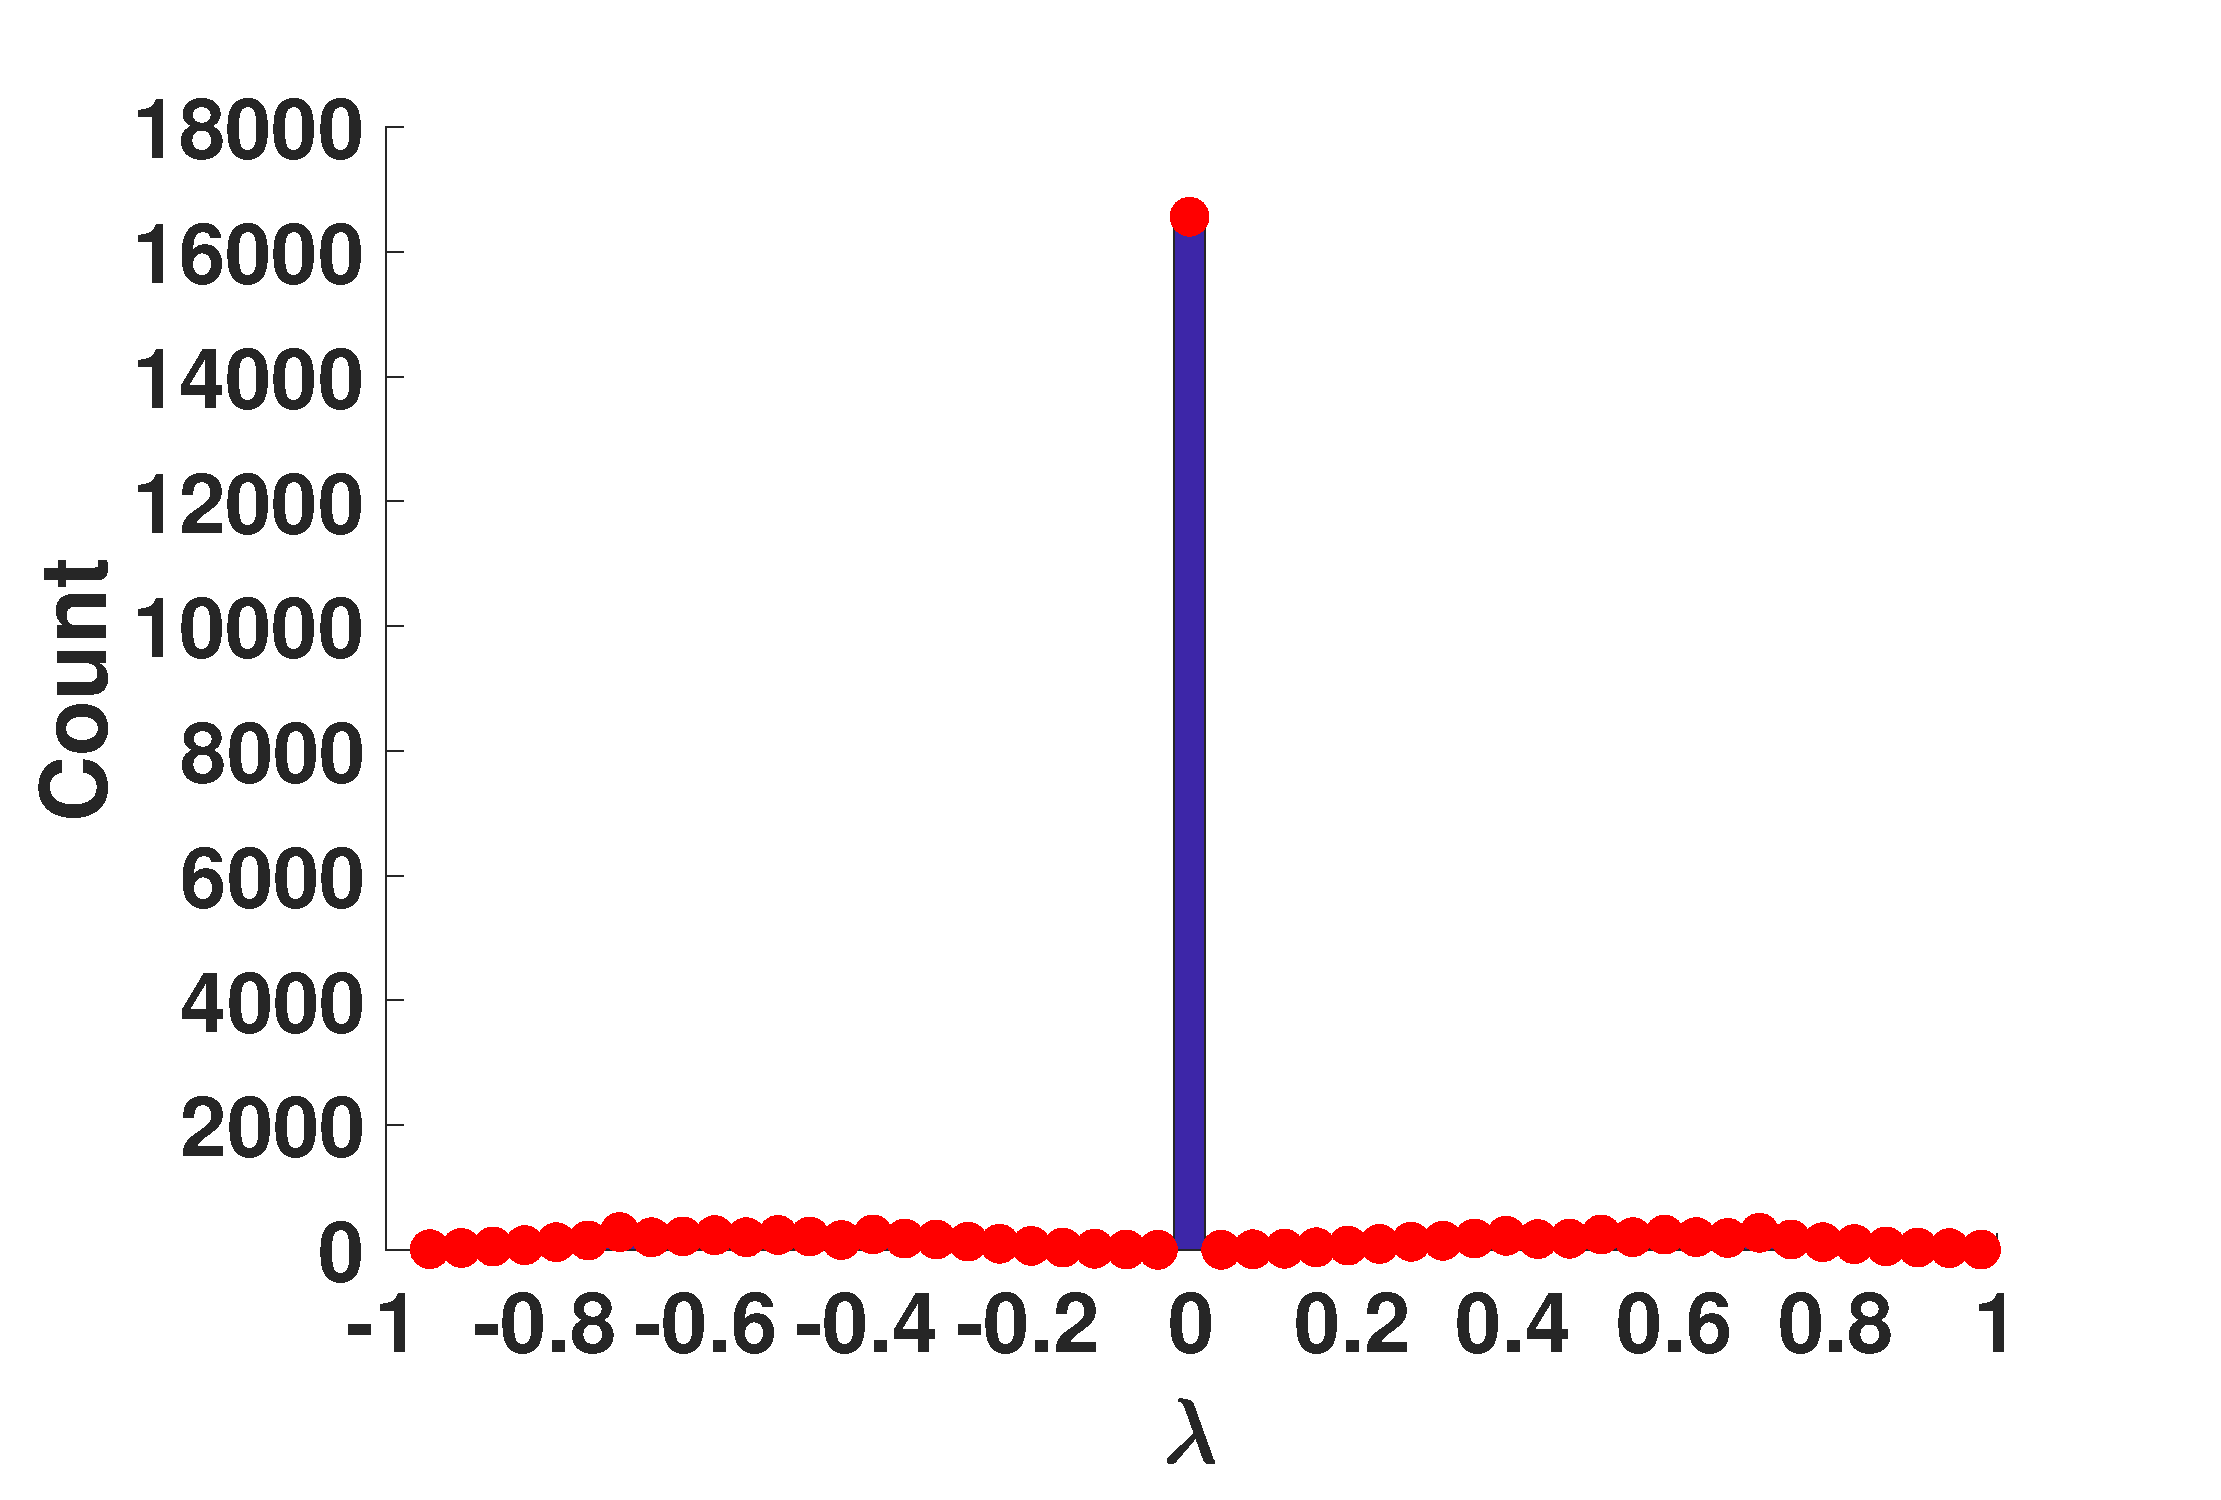
\includegraphics[width=\textwidth,trim = .4cm 0.5cm 3.5cm 1.3cm,clip]
      {./ndos/pics/as_caida_hist}
      \caption{Spectral Histogram}
      \label{fig:caida_full}
    \end{subfigure}
    %
    \begin{subfigure}{0.47\textwidth}
      \centering
      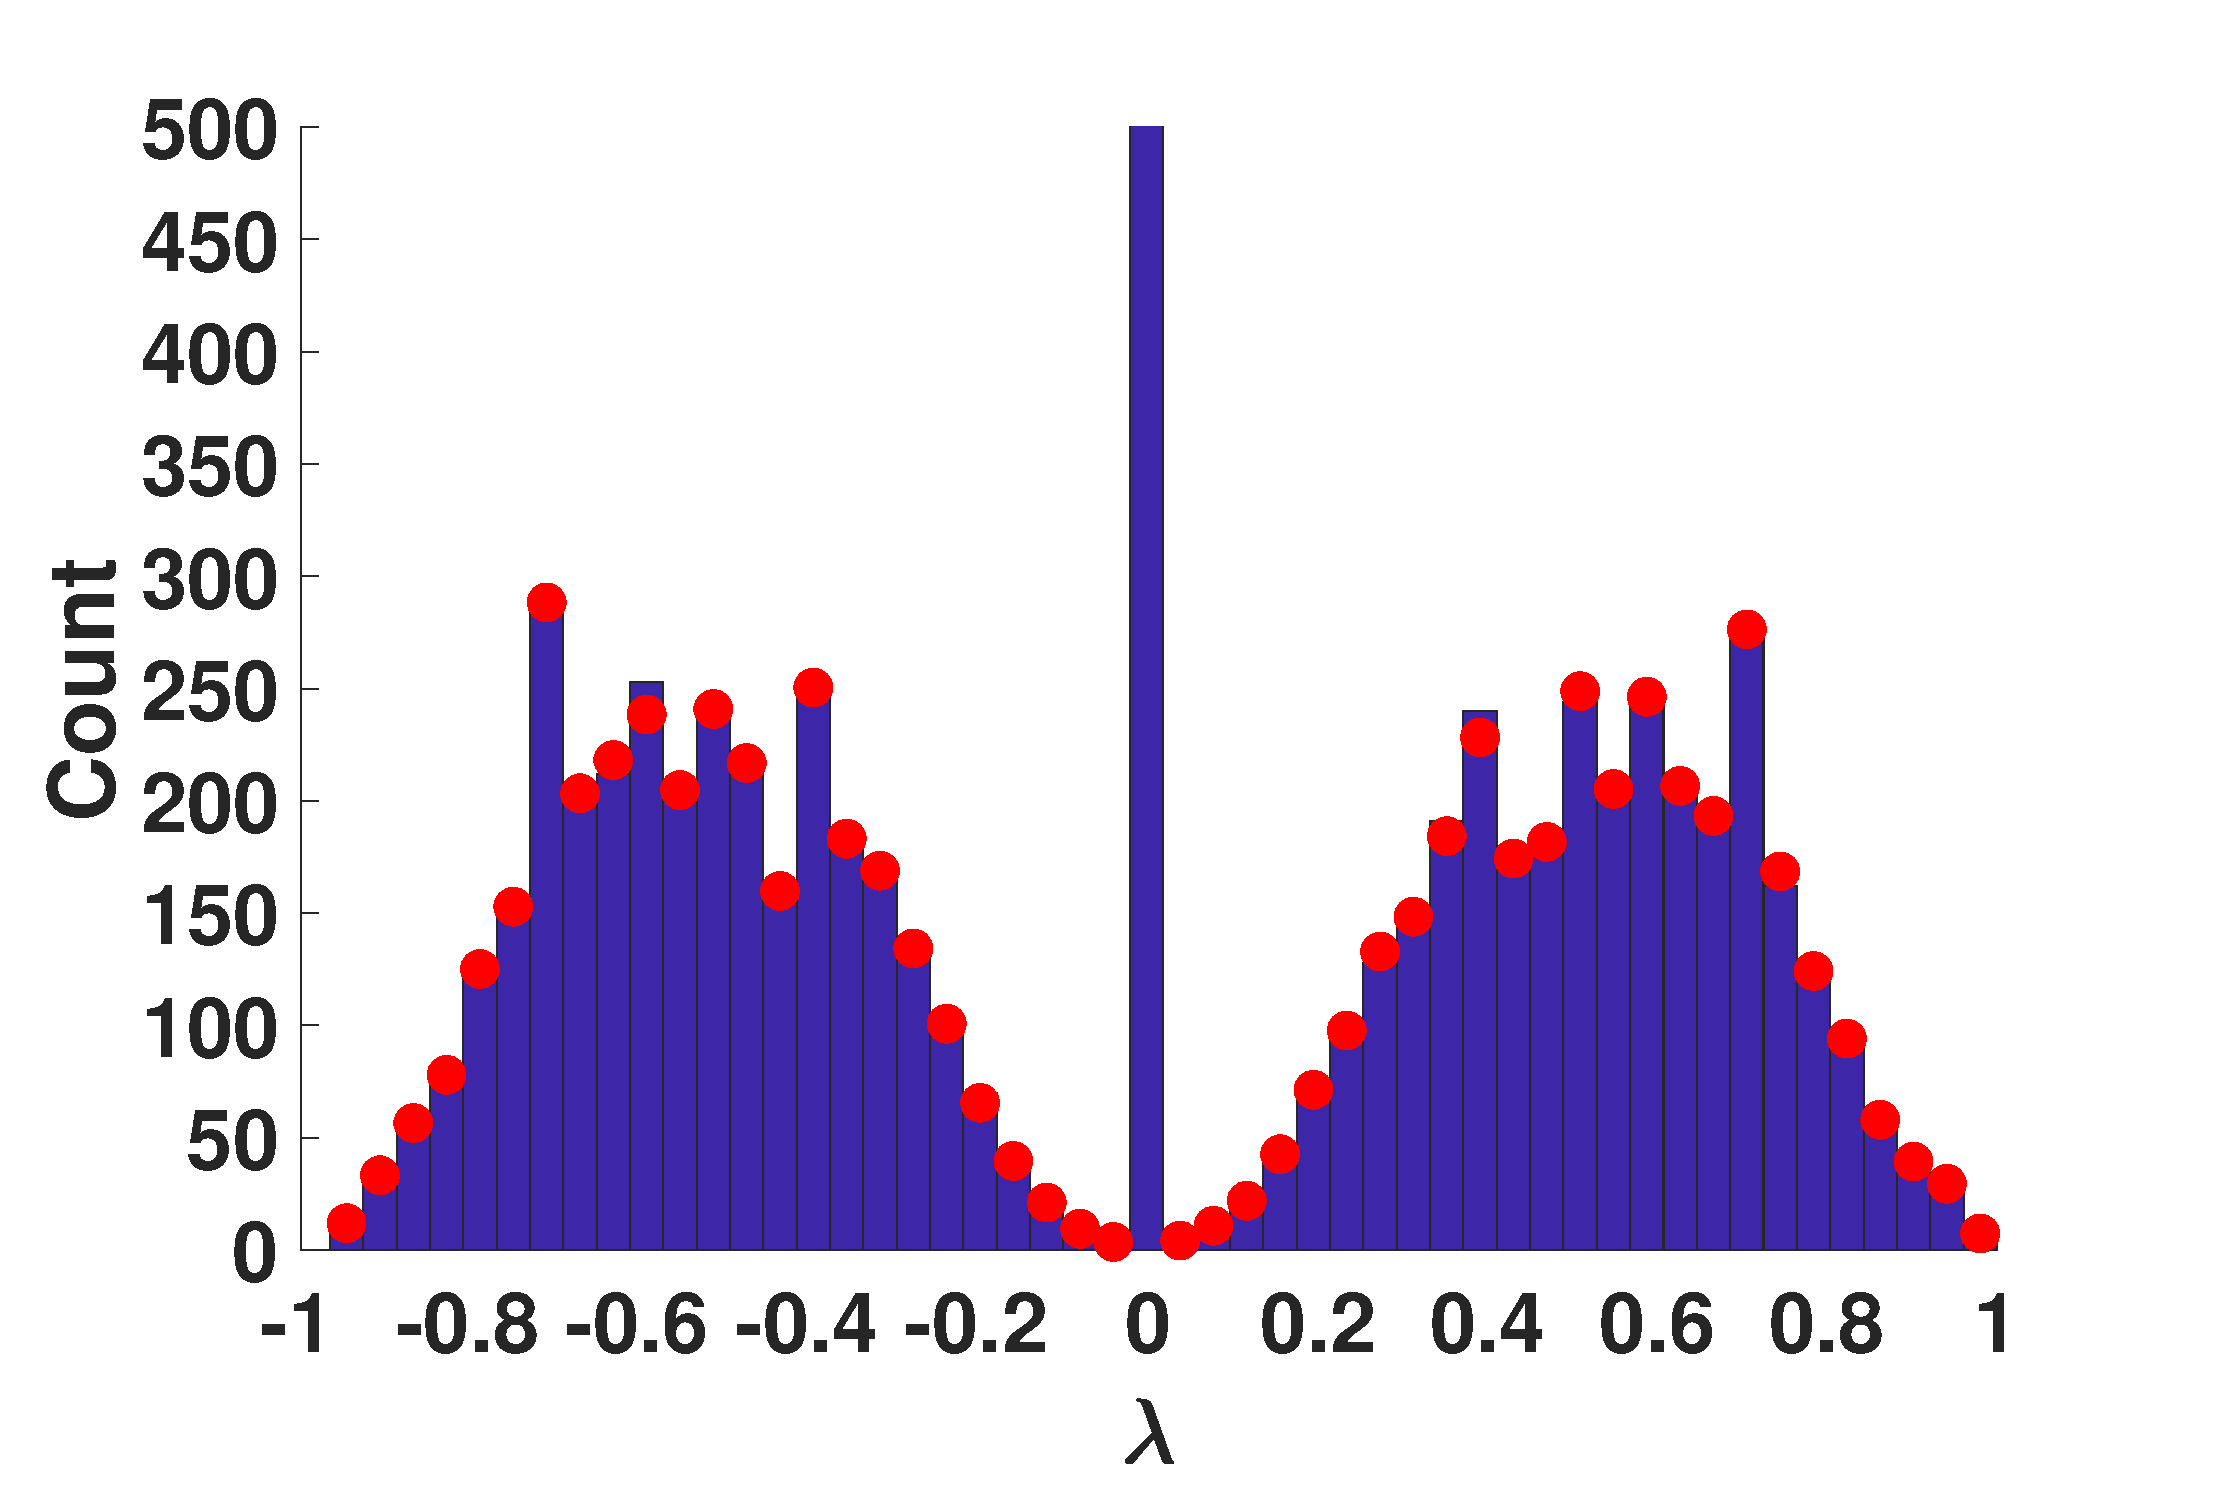
\includegraphics[width=\textwidth,trim = .4cm 0.5cm 3.5cm 1.3cm,clip]
      {./ndos/pics/as_caida_hist_zoom}
      \caption{Zoom-in View}
      \label{fig:caida_zoom}
    \end{subfigure}
    \caption{Spectral histogram for the normalized adjacency matrix for the
    CAIDA autonomous systems graph~\cite{caida2012}, an Internet topology with
    $22,965$ nodes and $47,193$ edges. Blue bars are the real spectrum, and red
    points are the approximated heights. (a) contains high multiplicity around
    eigenvalue $0$, so (b) zooms in to height between $[0,500]$.} 
    \label{fig:caida}
  \end{center}
\end{figure}
\vspace{-.5cm}

\section{Methods}\label{ndossec:met}
	The density of states plays a significant role in understanding electronic band
structure in solid state physics, and so several methods have been proposed in
that literature to estimate spectral densities. We review two such methods: the
kernel polynomial method (KPM) which involves a polynomial expansion of the
DOS/LDOS, and the Gauss Quadrature via Lanczos iteration (GQL). These methods
have not previously been applied in the network setting, though Cohen-Steiner et
al.~\cite{cohen2018approximating} have independently invented an approach
similar to KPM for the global DOS alone, albeit using a less numerically stable
polynomial basis (the power basis associated with random walks). We then
introduce a new direct nested dissection method for LDOS, as well as new
graph-specific modifications to improve the convergence of the KPM and GQL
approaches.

Throughout this section, $H$ denotes any symmetric matrix.

\subsection{Kernel Polynomial Method (KPM)}\label{subsec:kpm}

The Kernel Polynomial Method (KPM)~\cite{weisse2006kernel} approximates the
spectral density through an expansion in the dual basis of an orthogonal
polynomial basis. Traditionally, the Chebyshev basis $\{T_m\}$ is used because
of its connection to the best polynomial interpolation. Chebyshev approximation
requires the spectrum to be supported on the interval $[-1,1]$ for numerical
stability. However, this condition can be satisfied by any graph matrix after
shifting and rescaling:
\begin{equation}\label{eqn:shiftscale}
	\widetilde{H} = \frac{2H - (\lambda_{\max}(H)+\lambda_{\min}(H))}{\lambda_
	{\max}(H) - \lambda_{\min}(H)}\,.
\end{equation}
We can compute these extremal eigenvalues efficiently for our sparse matrix $H$,
so the pre-computation is not an issue~\cite{Parlett-1984-sparse}.

The Chebyshev polynomials $T_m(x)$ satisfy the recurrence
\begin{equation}\label{eq:cheb_3term}
	T_0(x) = 1,\; T_1(x) = x,\; T_{m+1}(x) = 2xT_m(x) - T_{m-1}(x)\,.
\end{equation}
They are orthogonal with respect to $w(x) =  2 / \left[(1+\delta_{0n})\pi
\sqrt{1-x^2}\right]$:
\begin{equation} \label{eqn:orth}
	\int_{-1}^1 w(x)T_m(x)T_n(x)dx = \delta_{mn}\,.
\end{equation}
(Here and elsewhere, $\delta_{ij}$ is the Kronecker delta: $1$ if $i = j$ and
$0$ otherwise.) Therefore, $T_m^\ast(x) = w(x)T_m(x)$ also forms the dual
Chebyshev basis. Using Eq. \ref{eqn:orth}, we can expand our DOS $\mu(\lambda)$
as
\begin{gather} \label{eqn:doscoeff}
\mu(\lambda) = \sum_{m=0}^\infty d_mT^\ast_m(\lambda)\,, \\
d_m = \int_{-1}^1T_m(\lambda)\mu(\lambda)d\lambda = \frac{1}{N}\sum_{i=1}^N 
T_m(\lambda_i) = \frac{1}{N}\tr(T_m(H))\,.
\end{gather}
Here, $T_m(H)$ is the $m$th Chebyshev polynomial of the matrix $H$. The last
equality comes from the spectral mapping theorem, which says that taking a
polynomial of $H$ maps the eigenvalues by the same polynomial. Similarly, we
express the PDOS $\mu_k(\lambda)$ as \begin{equation}\label{eqn:pdoscoeff}
d_{mk} = \int_{-1}^1 T_m(\lambda)\mu_k(\lambda)d\lambda = \sum_{i=1}^N |q_i(k)|
^2T_m(\lambda_i) = T_m(H)_{kk}.
\end{equation}

We want to efficiently extract the diagonal elements of the matrices $\{T_m
(H)\}$ without forming them explicitly; the key idea is to apply the stochastic
trace/diagonal estimation, proposed by Hutchinson~
\cite{hutchinson1990stochastic} and Bekas et al.~\cite{bekas2007estimator}.
Given a random probe vector $z$ such that $z_i$'s are i.i.d.~with mean $0$ and
variance $1$,
\begin{equation}\label{eq:probe_trace}
	\BBE[z^THz] = \sum_{i,j}H_{ij}\BBE[z_iz_j] = \tr(H)
\end{equation}
\begin{equation}\label{eq:probe_diag}
	\BBE[z\odot Hz] = \diag(H)
\end{equation}
where $\odot$ represents the Hadamard (elementwise) product. Choosing $N_z$
independent probe vectors $Z_j$, we obtain the unbiased estimator
\begin{equation}
	\tr(H) = \BBE[z^THz] \approx \frac{1}{N_z}\sum_{j=1}^{N_z}Z_j^THZ_j 
\end{equation}
and similarly for the diagonal. \citet{avron2011randomized} review many possible
choices of probes for \cref{eq:probe_trace,eq:probe_diag}; a common choice is
vectors with independent standard normal entries. Using the Chebyshev recurrence
(\cref{eq:cheb_3term}), we can compute the sequence $T_j(H)z$ for each probe at
a cost of one matrix-vector product per term, for a total cost of $\calO(
\abs{E}N_z)$ time per moment $T_m(H)$.

In practice, we only use a finite number of moments rather than an infinite
expansion. The number of moments required depends on the convergence rate of the
Chebyshev approximation for the class of functions DOS/LDOS is integrated with.
For example, the approximation error decays exponentially for test functions
that are smooth over the spectrum \cite{Trefethen-2013-ATAP}, so only a few
moments are needed. On the other hand, such truncation leads to Gibbs
oscillations that cause error in the interpolation ~\cite{Trefethen-2013-ATAP}.
However, to a large extent, we can use smoothing techniques such as Jackson
damping to resolve this issue ~\cite{jackson1911genauigkeit} (we will formalize
this in \cref{thm:Jackson_damping}).

\subsection{Gauss Quadrature and Lanczos (GQL)}
Golub and Meurant developed the well-known Gauss Quadrature and Lanczos (GQL)
algorithm to approximate bilinear forms for smooth functions of a matrix~
\cite{golub1997matrices}.  Using the same stochastic estimation from \S~
\ref{subsec:kpm}, we can also apply GQL to compute DOS.

For a starting vector $z$ and graph matrix $H$, Lanczos iterations after
$M$ steps produce a decomposition
\begin{equation}
	HZ_M = Z_M^T\Gamma_M + r_Me_M^T\,,
\end{equation}
where $Z_M^TZ_M = I_M$, $Z_M^Tr_M = 0$, and $\Gamma_M$ tridiagonal. GQL 
approximates $z^Tf(H)z$ with $\norm{z}^2e_1^Tf(T_M)e_1$, implying
\begin{equation}
	z^Tf(H)z = \sum_{i=1}^N \abs{z^Tq_i}^2f(\lambda_i) \approx \norm{z}^2\sum_
	{i=1}^M\abs{p_{i1}}^2f(\tau_i)\,,
\end{equation}
where $(\tau_1,p_1)\cdots,(\tau_M, p_M)$ are the eigenpairs of $\Gamma_M$. 
Consequently,
\begin{equation}
	\norm{z}^2\sum_{i=1}^M \abs{p_{i1}}^2\delta(\lambda-\tau_i)
\end{equation}
approximates the LDOS $\mu(\lambda; z)$.

Building upon the stochastic estimation idea and the invariance of probe 
vectors under orthogonal transformation, we have
\begin{equation}
	\BBE[\mu(\lambda;z)] = \sum_{i=1}^N \delta(\lambda-\lambda_i) = N\mu
	(\lambda)\,.
\end{equation}
Hence 
\begin{equation}
	\mu(\lambda)\approx\sum_{i=1}^M |p_{i1}|^2\delta(\lambda-\tau_i)\,.
\end{equation}
The approximate generalized function is exact when applied to polynomials of
degree $\Leq 2M+1$. Furthermore, if we let $z = e_k$ then GQL also provides an
estimation for the PDOS $\mu_k(\lambda)$. Estimation from GQL can also be
converted to Chebyshev moments if needed.

\subsection{Nested Dissection (ND)}

The estimation error via Monte Carlo method intrinsically decays at the rate
$\calO(1 /\!\!\sqrt{N_z})$, where $N_z$ is the number of random probing vectors.
Hence, we have to tolerate the higher variance when increasing the number of
probe vectors becomes too expensive. This is particularly problematic when we
try to compute the PDOS for all nodes using the stochastic diagonal estimator.
Therefore, we introduce an alternative divide-and-conquer  method, which
computes more accurate PDOS for any set of nodes at a cost comparable to the
stochastic approach in practice.

Suppose the graph can be partitioned into two subgraphs by removal of a small
vertex separator.  Permuting the vertices so that the two partitions appear
first, followed by the separator vertices. Up to vertex permutations, we can
rewrite $H$ in block form as
\begin{equation}\label{eqn:dissection}
	H = \begin{bmatrix}
	H_{11} & 0 & H_{13}\\
	0 & H_{22} & H_{23}\\
	H_{13}^T & H_{23}^T & H_{33}
	\end{bmatrix},
\end{equation}
where the indices indicate the groups identities. Leveraging this structure, we
can update the recurrence relation for Chebyshev polynomials to become
\begin{equation}\label{eqn:ndcheb}
	T_{m+1}(H)_{11} = 2H_{11}T_m(H)_{11} - T_{m-1}(H)_{11} + 2H_{13}T_m(H)_{31}\,.
\end{equation}

Recursing on the partitioning will lead to a nested dissection, after which we
will use direct computation on sufficiently small sub-blocks. We denote the
indexing of each partition with $I^{(t)}_p = I^{(t)}_s\bigcup I^{
(t)}_\ell\bigcup I^{(t)}_r$, which represents all nodes in the current
partition, the separators, and two sub-partitions, respectively. For the
separators, \cref{eqn:ndcheb} leads to
\begin{align}\label{eqn:ndchebsep}
	&T_{m+1}(H)(I^{(t)}_p,I^{(t)}_s) = 2H(I^{(t)}_p, I^{(t)}_p)T_m(H)(I^{(t)}_p,
	I^{(t)}_s) \nonumber\\
	&-T_{m-1}(H)(I^{(t)}_p,I^{(t)}_s) + 2\sum_{t'\in S_t}H(I^{(t)}_p,I^{(t')}_s)
	T_m(H)(I^{(t')}_s, I^{(t)}_s)\,,
\end{align}
where $S_t$ is the path from partition $t$ to the root; and for the leaf
blocks, $I^{(t)}_s = I^{(t)}_p$ in \cref{eqn:ndchebsep}. The result is 
\cref{alg:ndpdos}.

\begin{algorithm}
	\SetKwInput{KwInput}{Input}
	\SetKwInput{KwOutput}{Output}
	\DontPrintSemicolon
		\KwInput{Symmetric graph matrix $H$ with eigenvalues in $[-1,1]$}
		\KwOutput{$C\in\BBR^{N\times M}$ where $c_{ij}$ is the $j$-th Chebyshev
		moment for $i$-th node.}
		\Begin{
			Obtain partitions $\{I^{(t)}_p\}$ in a tree structure through
			multilevel nested dissection.\;
			\For{$m=1$ \textbf{to} $M$}{
				Traverse partition tree in pre-order:\;
				\quad Compute the separator columns with \cref{eqn:ndchebsep}.\;
				\quad \If{$I^{(t)}_p$ is a leaf block}{Compute the diagonal entries
				with equation (\ref{eqn:ndchebsep}).}
			}
		}
	\caption{Nested Dissection for PDOS Approximation}
	\label{alg:ndpdos}        
\end{algorithm}

The multilevel nested dissection process itself has a well-established
algorithm by \citeauthor{karypis1998fast}, and efficient implementation is
available in \texttt{METIS}~\cite{karypis1998fast}. Note that this approach is
only viable when the graph can be partitioned with a separator of small size.
Empirically, we observe this assumption to hold for many real-world networks.
The biggest advantage of this approach is we can very efficiently obtain PDOS
estimation for a subset of nodes with much better accuracy than KPM.


\subsection{Motif Filtering}

In many graphs, there are large spikes around particular eigenvalues; for
example, see \cref{fig:caida}. This phenomenon affects the accuracy of DOS
estimation in two ways. First, the singularity-like behavior means we need many
more moments to obtain a good approximation in polynomial basis. Secondly, due
to the equi-oscillation property of Chebyshev approximation, error in
irregularities (say, at a point of high concentration in the spectral density),
spreads to other parts of the spectrum. This is a problem in our case, as the
spectral density of real-world networks are far from uniform.

High multiplicity eigenvalues are typically related to local symmetries in a
graph. The most prevalent example is two dangling nodes attached to the same
neighbor as shown in \cref{fig:motif_0}, which accounts for most eigenvalues
around $0$ for (normalized) adjacency matrix with a localized eigenvector taking
value $+1$ on one node and $-1$ on the other. In addition, we list a few more
motifs in \cref{fig:motifs} that appear most frequently in real-world graphs.
All of them can be associated with specific eigenvalues, and we include the
corresponding ones in normalized adjacency matrix for our example.

\begin{figure}[htp]
	\begin{center}
  \begin{subfigure}{\textwidth}
  	\centering
		\begin{tikzpicture}[remember picture, overlay]
			\node[draw,line width=1mm,circle,inner sep=1mm] (A) at (-3.5,0) 
			{${\color{blue}\bm{+1}}$};
			\node[draw,line width=1mm,circle,inner sep=1mm] (B) at (-1.5,0)
			{${\color{red}\bm{-1}}$};
			\node[draw,line width=1mm,fill=gray,circle,inner sep=3mm] (C) at 
			(-2.5,-1) {};
			\node[draw,line width=1mm,circle,inner sep=1mm] (D) at (1.5,0)
			{${\color{red}\bm{-1}}$};
			\node[draw,line width=1mm,circle,inner sep=1mm] (E) at (3.5,0)
			{${\color{blue}\bm{+1}}$};
			\node[draw,line width=1mm,circle,inner sep=1mm] (F) at (5.5,0)
			{${\color{red}\bm{-1}}$};
			\node[draw,line width=1mm,fill=gray,circle,inner sep=3mm] (G) at 
			(2.5,-1) {};
			\node[draw,line width=1mm,fill=gray,circle,inner sep=3mm] (H) at 
			(4.5,-1) {};

			\draw[line width=1mm] (A)--(C);
			\draw[line width=1mm] (B)--(C);
			\draw[line width=1mm, loosely dashed] (-4,-2)--(C);
			\draw[line width=1mm, loosely dashed] (-1,-2)--(C);
			\draw[line width=1mm] (D)--(G);
			\draw[line width=1mm] (E)--(G);
			\draw[line width=1mm] (E)--(H);
			\draw[line width=1mm] (F)--(H);
			\draw[line width=1mm, loosely dashed] (1,-2)--(G);
			\draw[line width=1mm, loosely dashed] (4,-2)--(G);
			\draw[line width=1mm, loosely dashed] (3,-2)--(H);
			\draw[line width=1mm, loosely dashed] (6,-2)--(H);
		\end{tikzpicture}
		\vspace{2.5cm}
		\caption{$\lambda=0$}\label{fig:motif_0}
	\end{subfigure}
  %
  \begin{subfigure}{\textwidth}
  	\centering
		\begin{tikzpicture}[remember picture, overlay]
			\node[draw,line width=1mm,circle,inner sep=1mm] (A) at (-5,-1) 
			{${\color{blue}\bm{+1}}$};
			\node[draw,line width=1mm,circle,inner sep=1mm] (B) at (-3.75,-1)
			{${\color{green}\bm{\pm 1}}$};
			\node[draw,line width=1mm,circle,inner sep=1mm] (C) at (-2.25,-1)
			{${\color{red}\bm{-1}}$};
			\node[draw,line width=1mm,circle,inner sep=1mm] (D) at (-1,-1)
			{${\color{burgundy}\bm{\mp 1}}$};
			\node[draw,line width=1mm,fill=gray,circle,inner sep=3mm] (E) at 
			(-3.75,-2.5) {};
			\node[draw,line width=1mm,fill=gray,circle,inner sep=3mm] (F) at 
			(-2.25,-2.5) {};
			\node[draw,line width=1mm,circle,inner sep=1mm] (G) at (1,-1) 
			{${\color{green}\bm{\pm1}}$};
			\node[draw,line width=1mm,circle,inner sep=1mm] (H) at (2.25,-1)
			{${\color{blue}\bm{+1}}$};
			\node[draw,line width=1mm,circle,inner sep=1mm] (I) at (3.75,-1)
			{${\color{red}\bm{-1}}$};
			\node[draw,line width=1mm,circle,inner sep=1mm] (J) at (5,-1)
			{${\color{burgundy}\bm{\mp 1}}$};
			\node[draw,line width=1mm,fill=gray,circle,inner sep=3mm] (K) at 
			(1.5,-2.5) {};
			\node[draw,line width=1mm,fill=gray,circle,inner sep=3mm] (L) at 
			(3,-2.5) {};
			\node[draw,line width=1mm,fill=gray,circle,inner sep=3mm] (M) at 
			(4.5,-2.5) {};

			\draw[line width=1mm] (A)--(E);
			\draw[line width=1mm] (C)--(E);
			\draw[line width=1mm] (A)--(B);
			\draw[line width=1mm] (C)--(D);
			\draw[line width=1mm] (B)--(F);
			\draw[line width=1mm] (D)--(F);
			\draw[line width=1mm, loosely dashed] (-4.75,-3.5)--(E);
			\draw[line width=1mm, loosely dashed] (-3.25,-3.5)--(F);
			\draw[line width=1mm, loosely dashed] (-2.25,-3.5)--(E);
			\draw[line width=1mm, loosely dashed] (-1.25,-3.5)--(F);

			\draw[line width=1mm] (G)--(H);
			\draw[line width=1mm] (I)--(J);
			\draw[line width=1mm] (H)--(K);
			\draw[line width=1mm] (H)--(L);
			\draw[line width=1mm] (H)--(M);
			\draw[line width=1mm] (I)--(K);
			\draw[line width=1mm] (I)--(L);
			\draw[line width=1mm] (I)--(M);
			\draw[line width=1mm, loosely dashed] (0.5,-3.5)--(K);
			\draw[line width=1mm, loosely dashed] (2.5,-3.5)--(K);
			\draw[line width=1mm, loosely dashed] (2,-3.5)--(L);
			\draw[line width=1mm, loosely dashed] (4,-3.5)--(L);
			\draw[line width=1mm, loosely dashed] (3.5,-3.5)--(M);
			\draw[line width=1mm, loosely dashed] (5.5,-3.5)--(M);
		\end{tikzpicture}
		\vspace{4cm}
		\caption{$\lambda = \pm 1/2$}
		\label{fig:motif_pmhalf}
  \end{subfigure}
  %
  \begin{subfigure}{0.47\textwidth}
  	\centering
		\begin{tikzpicture}[remember picture, overlay]
			\node[draw,line width=1mm,circle,inner sep=1mm] (A) at (-1,-1) 
			{${\color{blue}\bm{+1}}$};
			\node[draw,line width=1mm,circle,inner sep=1mm] (B) at (1,-1)
			{${\color{red}\bm{-1}}$};
			\node[draw,line width=1mm,fill=gray,circle,inner sep=3mm] (C) at 
			(0,-2) {};

			\draw[line width=1mm] (A)--(C);
			\draw[line width=1mm] (B)--(C);
			\draw[line width=1mm] (A)--(B);
			\draw[line width=1mm, loosely dashed] (-1.5,-3)--(C);
			\draw[line width=1mm, loosely dashed] (1.5,-3)--(C);
		\end{tikzpicture}
		\vspace{3.5cm}
		\caption{$\lambda = -1/2$}\label{fig:motif_minushalf}
  \end{subfigure}
  \hspace{-1cm}
  \begin{subfigure}{0.47\textwidth}
  	\centering
		\begin{tikzpicture}[remember picture, overlay]
			\node[draw,line width=1mm,circle,inner sep=1mm] (A) at (-2.5,-2) 
			{${\color{green}\bm{\pm1}}$};
			\node[draw,line width=1mm,circle,inner sep=1mm] (B) at (-1.25,-1)
			{\small${\color{blue}\bm{+1/\!\!\sqrt{2}}}$};
			\node[draw,line width=1mm,circle,inner sep=1mm] (C) at (1.25,-1)
			{\small$\selectfont{\color{blue}\bm{+1/\!\!\sqrt{2}}}$};
			\node[draw,line width=1mm,circle,inner sep=1mm] (D) at (2.5,-2)
			{${\color{green}\bm{\pm 1}}$};
			\node[draw,line width=1mm,fill=gray,circle,inner sep=3mm] (E) at 
			(0,-2) {};

			\draw[line width=1mm] (A)--(B);
			\draw[line width=1mm] (B)--(E);
			\draw[line width=1mm] (C)--(D);
			\draw[line width=1mm] (C)--(E);
			\draw[line width=1mm, loosely dashed] (-1.5,-3)--(E);
			\draw[line width=1mm, loosely dashed] (1.5,-3)--(E);
		\end{tikzpicture}
		\vspace{3.5cm}
		\caption{$\lambda = \pm1/\sqrt{2}$}\label{fig:motif_sqrt2}
  \end{subfigure}
  \caption{Common motifs (induced subgraphs) in graph data that result in
  localized spikes in the spectral density. Each motif generates a specific
  eigenvalue with locally-supported eigenvectors. Here we uses the normalized
  adjacency matrix to represent the graph, although we can perform the same
  analysis for the adjacency, Laplacian, or normalized Laplacian (only the
  eigenvalues would be different). The eigenvectors are supported only on the
  labeled nodes.}\label{fig:motifs}
  \end{center}
\end{figure}

To detect these motifs in large graphs, we deploy a randomized hashing
technique. Given a random vector $z$, the hashing weight $w=Hz$ encodes all
the neighborhood information of each node. To find node copies (left in Figure 
\ref{fig:motif_0}), we seek pairs $(i, j)$ such that $w_i=w_j$; with high
probability, this only happens when $v_i$ and $v_j$ share the same neighbors.
Similarly, all motifs in Figure \ref{fig:motifs} can be characterized by union
and intersection of neighborhood lists.

After identifying motifs, we need only approximate the (relatively smooth)
density of the remaining spectrum.  The eigenvectors associated with these
remaining non-motif eigenvalues must be constant across cycles in the canonical
decomposition of the associated permutations.  Let $P \in \BBR^{N \times r}$
denote an orthonormal basis for the space of such vectors formed from columns of
the identity and (normalized) indicators for nodes cyclically permuted by the
motif.  The matrix $H_r = P^T H P$ then has identical eigenvalues to $H$, except
with all the motif eigenvalues omitted. We may form $H_r$ explicitly, as it has
the same sparsity structure as $H$ but with a supernode replacing the nodes in
each instance of a motif cycle; or we can achieve the same result by replacing
each random probe $Z$ with the projected probe $Z_r = PP^T Z$ at an additional
cost of $O(N_{\mathrm{motif}})$ per probe, where $N_{\mathrm{motif}}$ is the
number of nodes involved in motifs.

The motif filtering method essentially allow us to isolate the spiky components
from the spectrum. As a result, we are able to obtain a more accurate
approximation using fewer Chebyshev moments. Figure \ref{fig:motif_filt}
demonstrates the improvement on the approximation as we procedurally filter out
motifs at $0$, $-1/3$, $-1/2$, and $-1/4$. The eigenvalue $-1/m$ can be
generated by an edge attached to the graph through $m-1$ nodes, similar to
motif (\ref{fig:motif_minushalf}).
\begin{figure}
	\begin{subfigure}{0.47\textwidth}
    \centering  
    \captionsetup{justification=centering}
    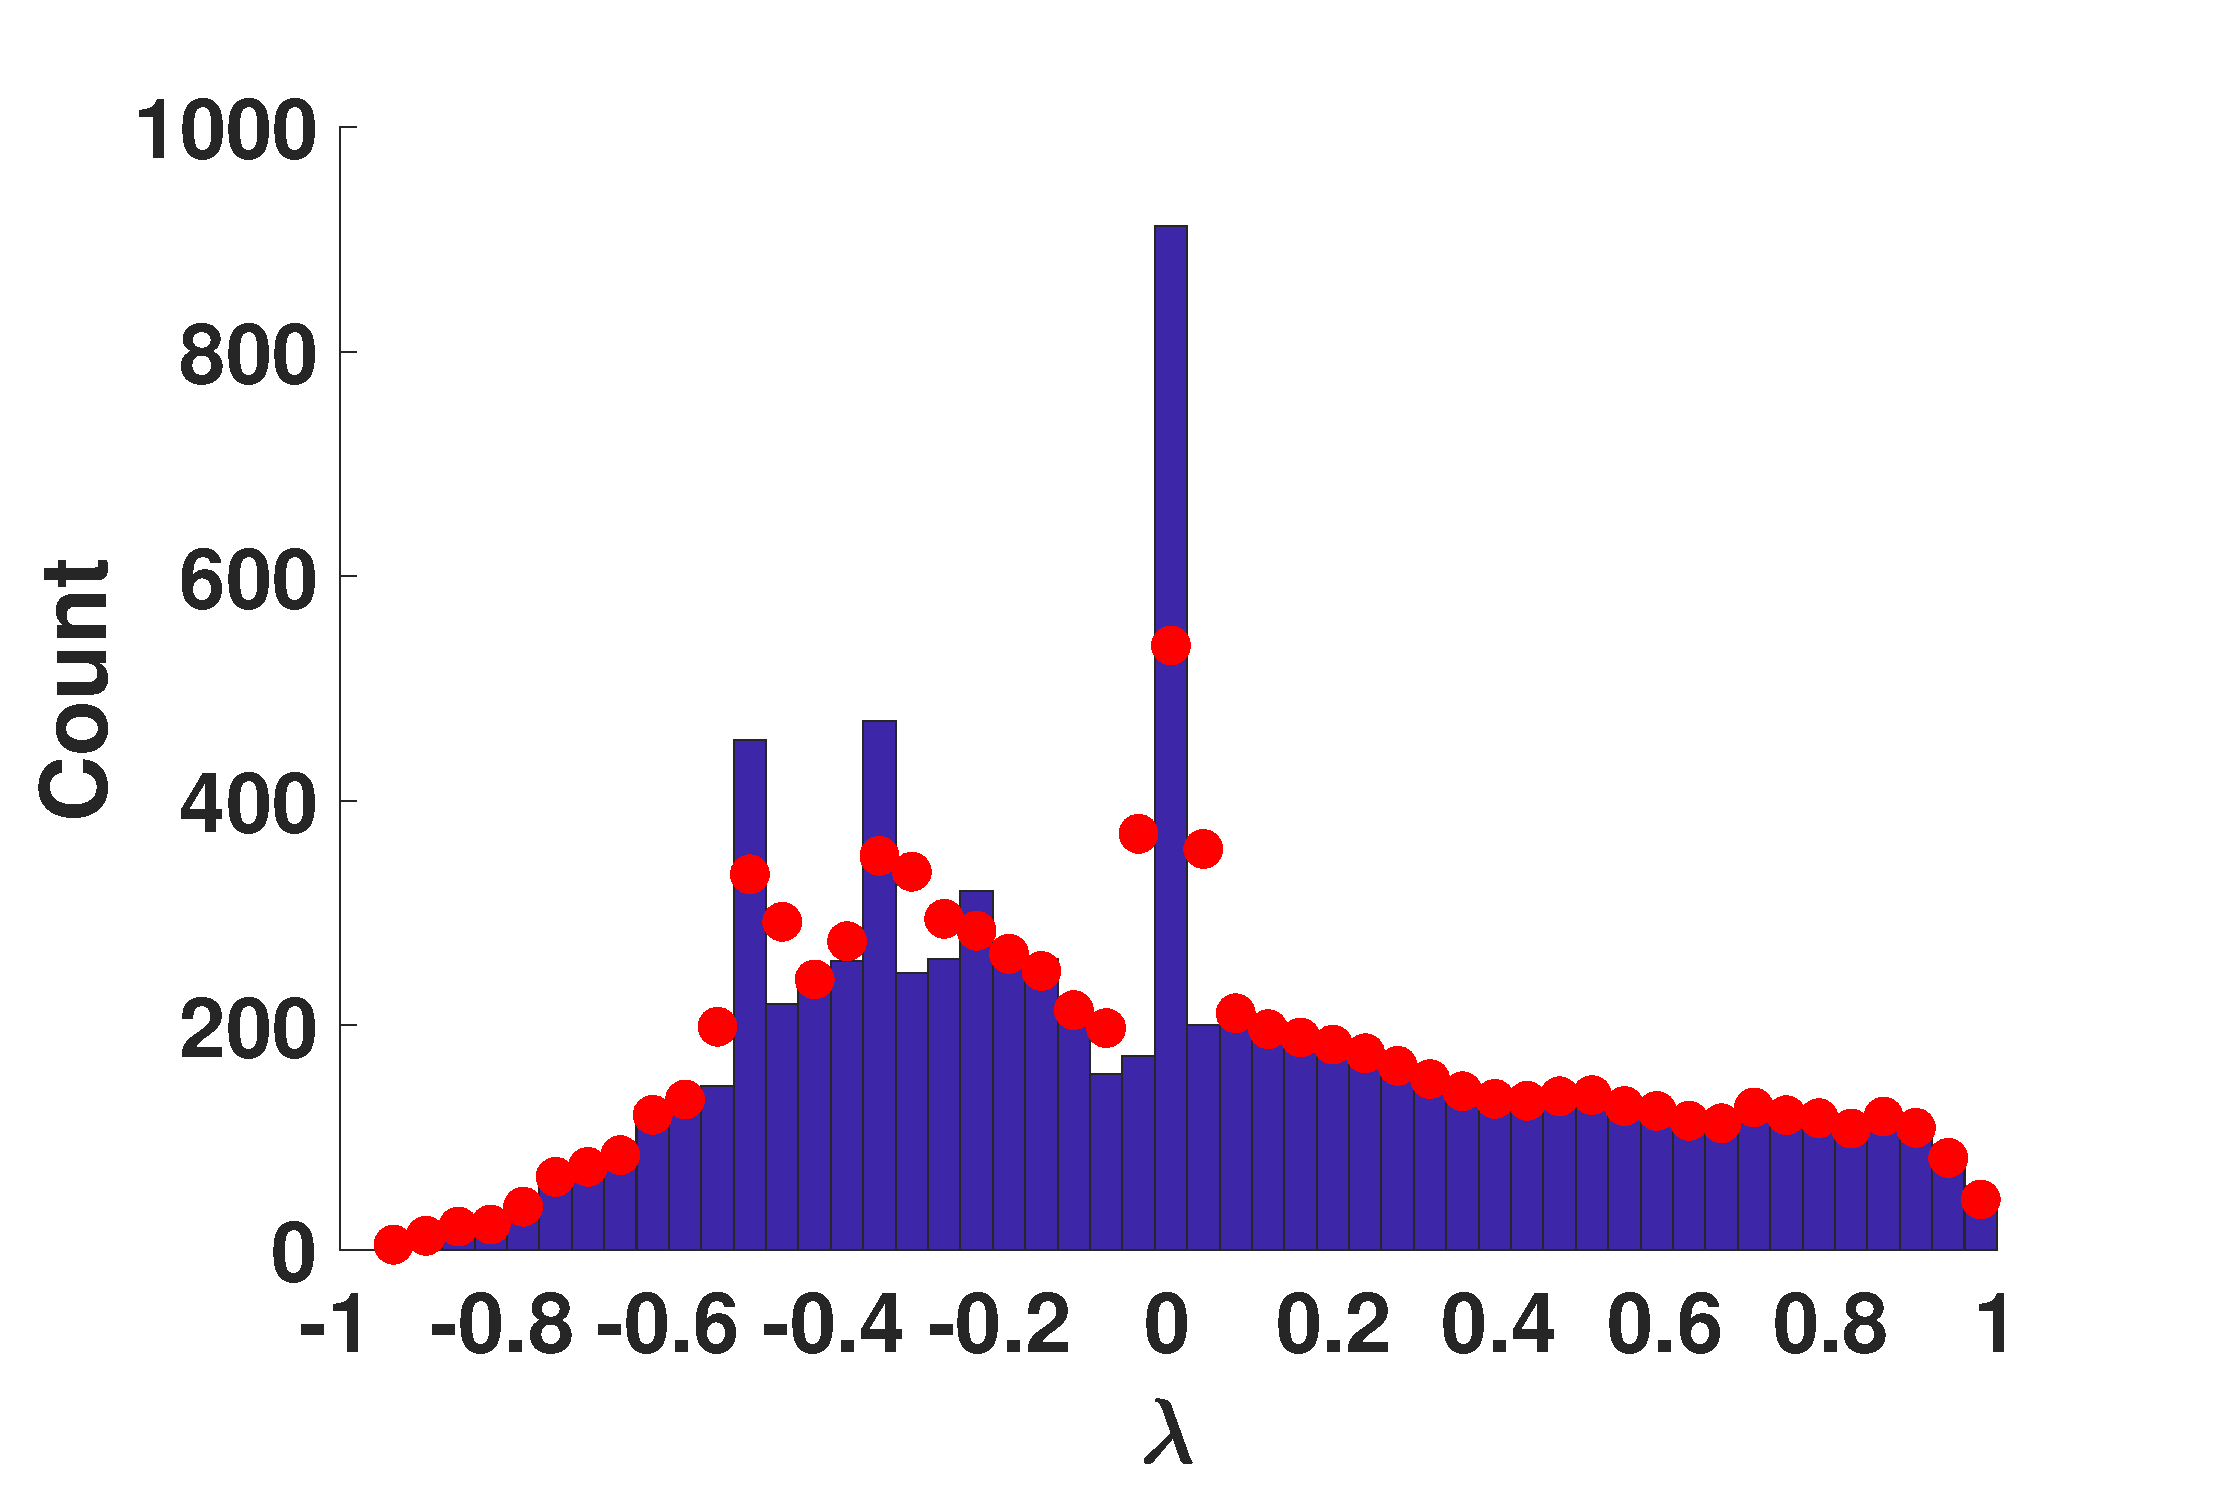
\includegraphics[width=\textwidth,trim = .3cm 0.5cm 3.2cm 1.3cm,clip]
    {./ndos/pics/hepth_nofilter}
    \caption{No Filter}\label{fig:hepth_0filt}
  \end{subfigure}
  %
  \begin{subfigure}{0.47\textwidth}
    \centering
    \captionsetup{justification=centering}
    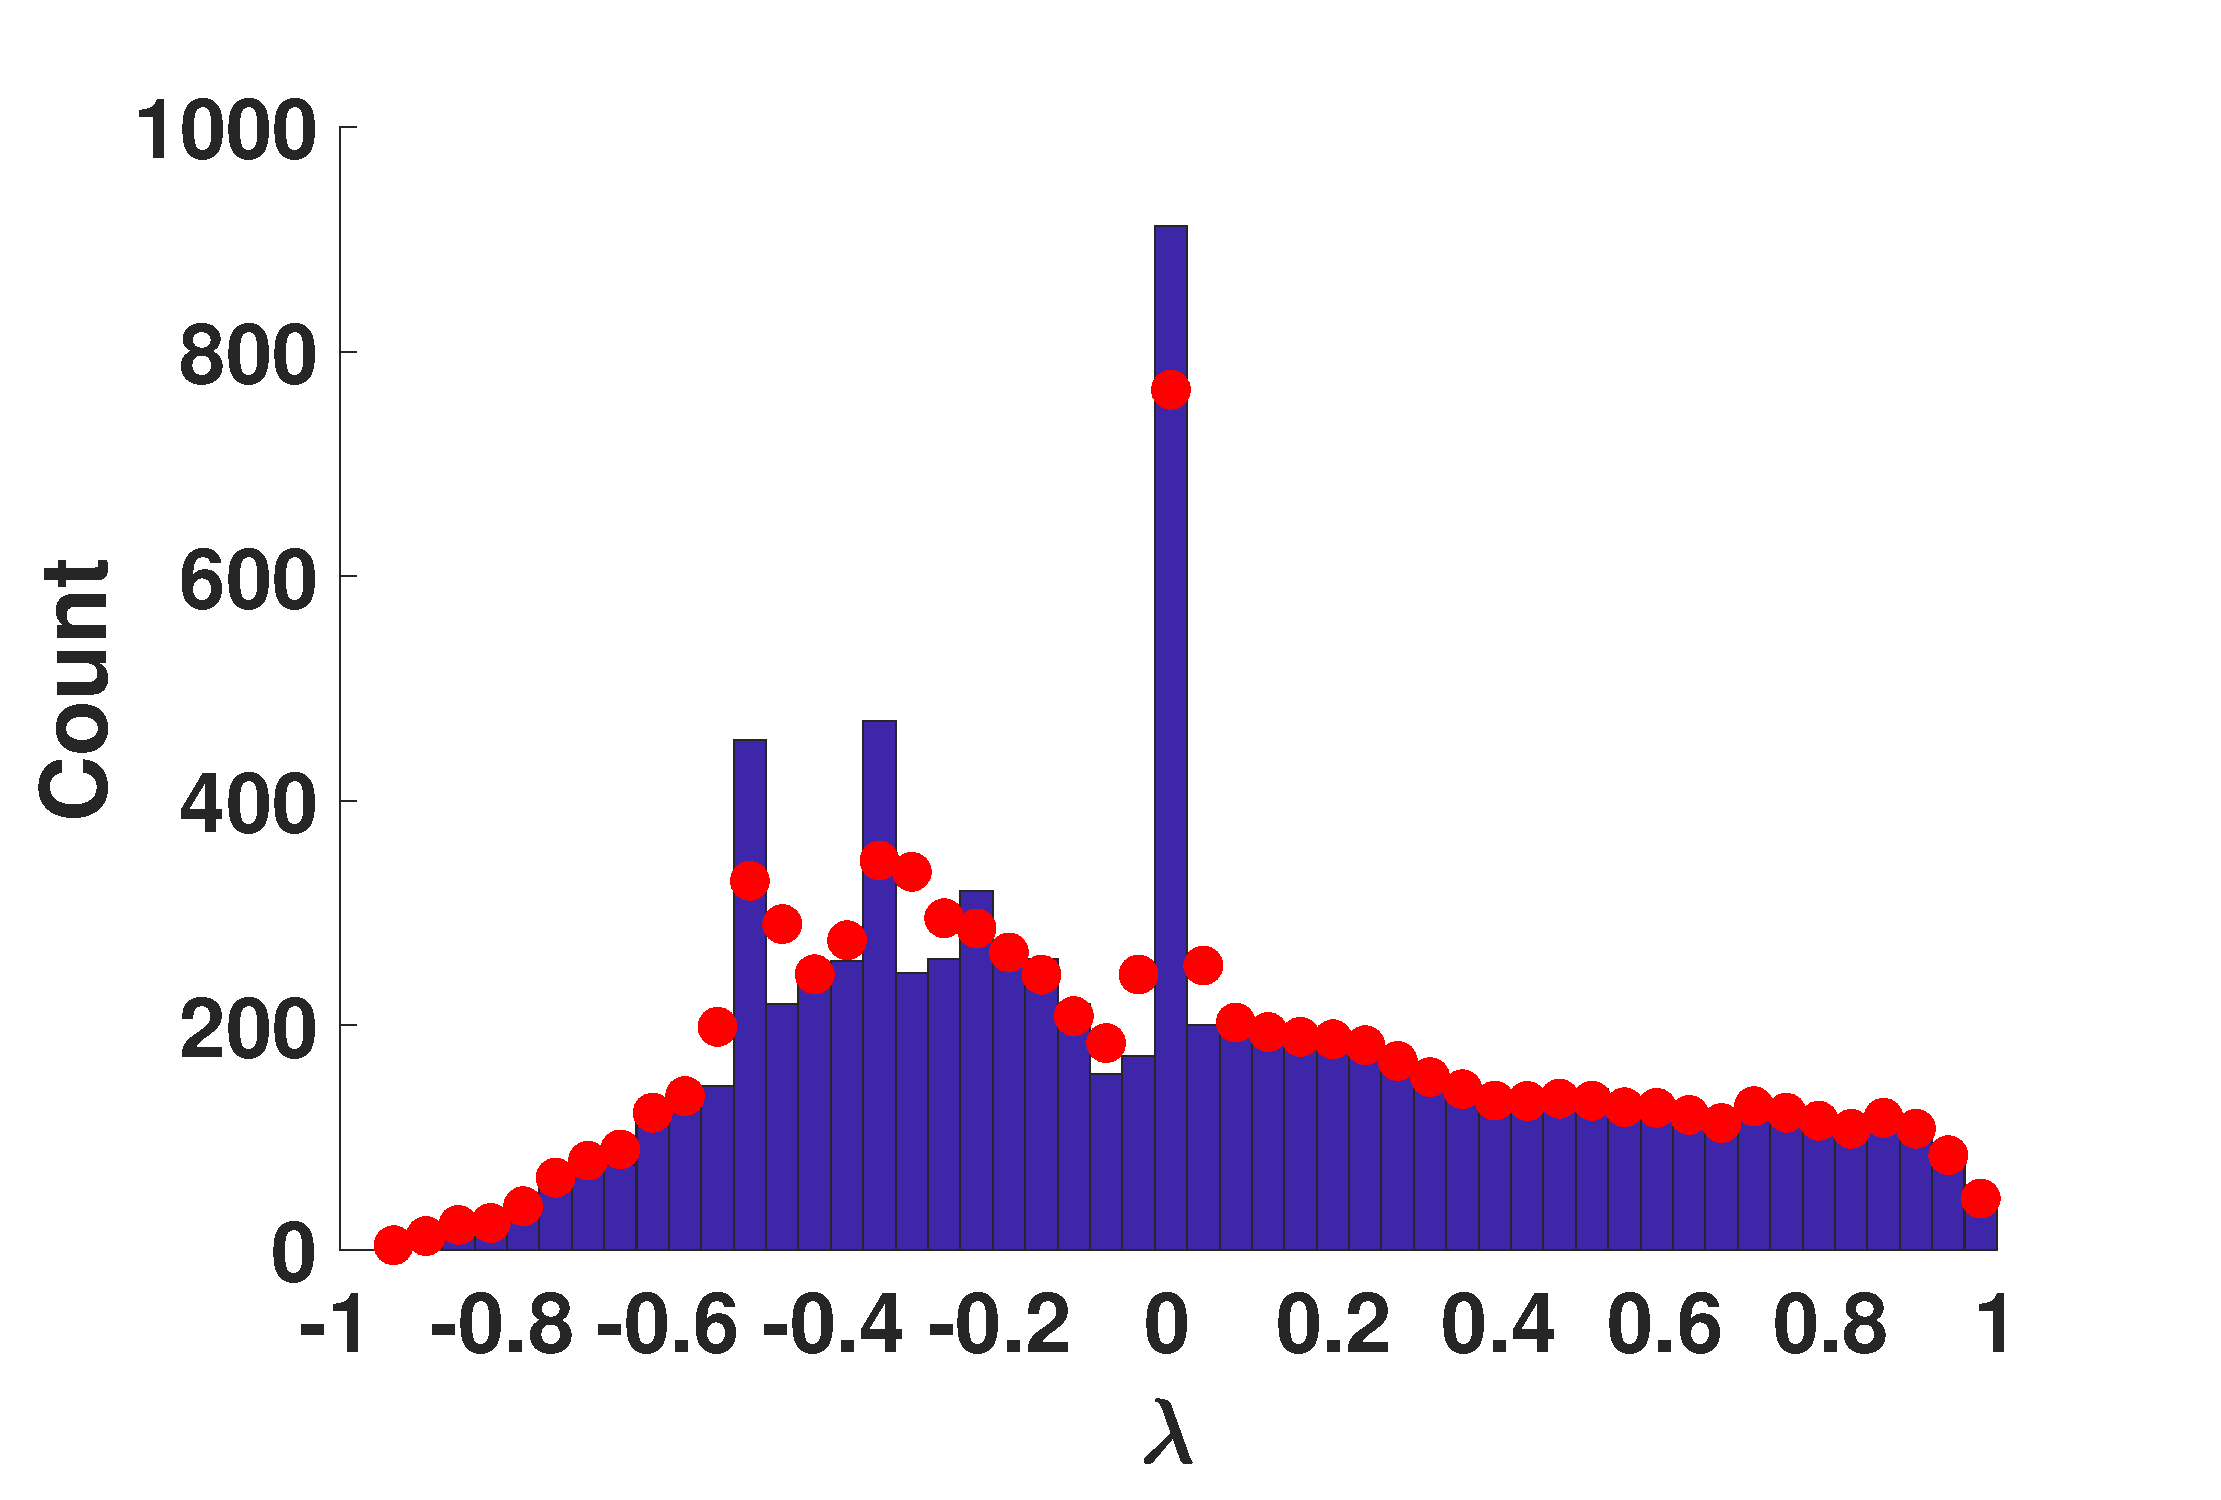
\includegraphics[width=\textwidth,trim = .3cm 0.5cm 3.2cm 1.3cm,clip]
    {./ndos/pics/hepth_onefilter}
    \caption{Filter at $\lambda=0$}\label{fig:hepth_1filt}
  \end{subfigure}
  %
  \begin{subfigure}{0.47\textwidth}
    \centering
    \captionsetup{justification=centering}
    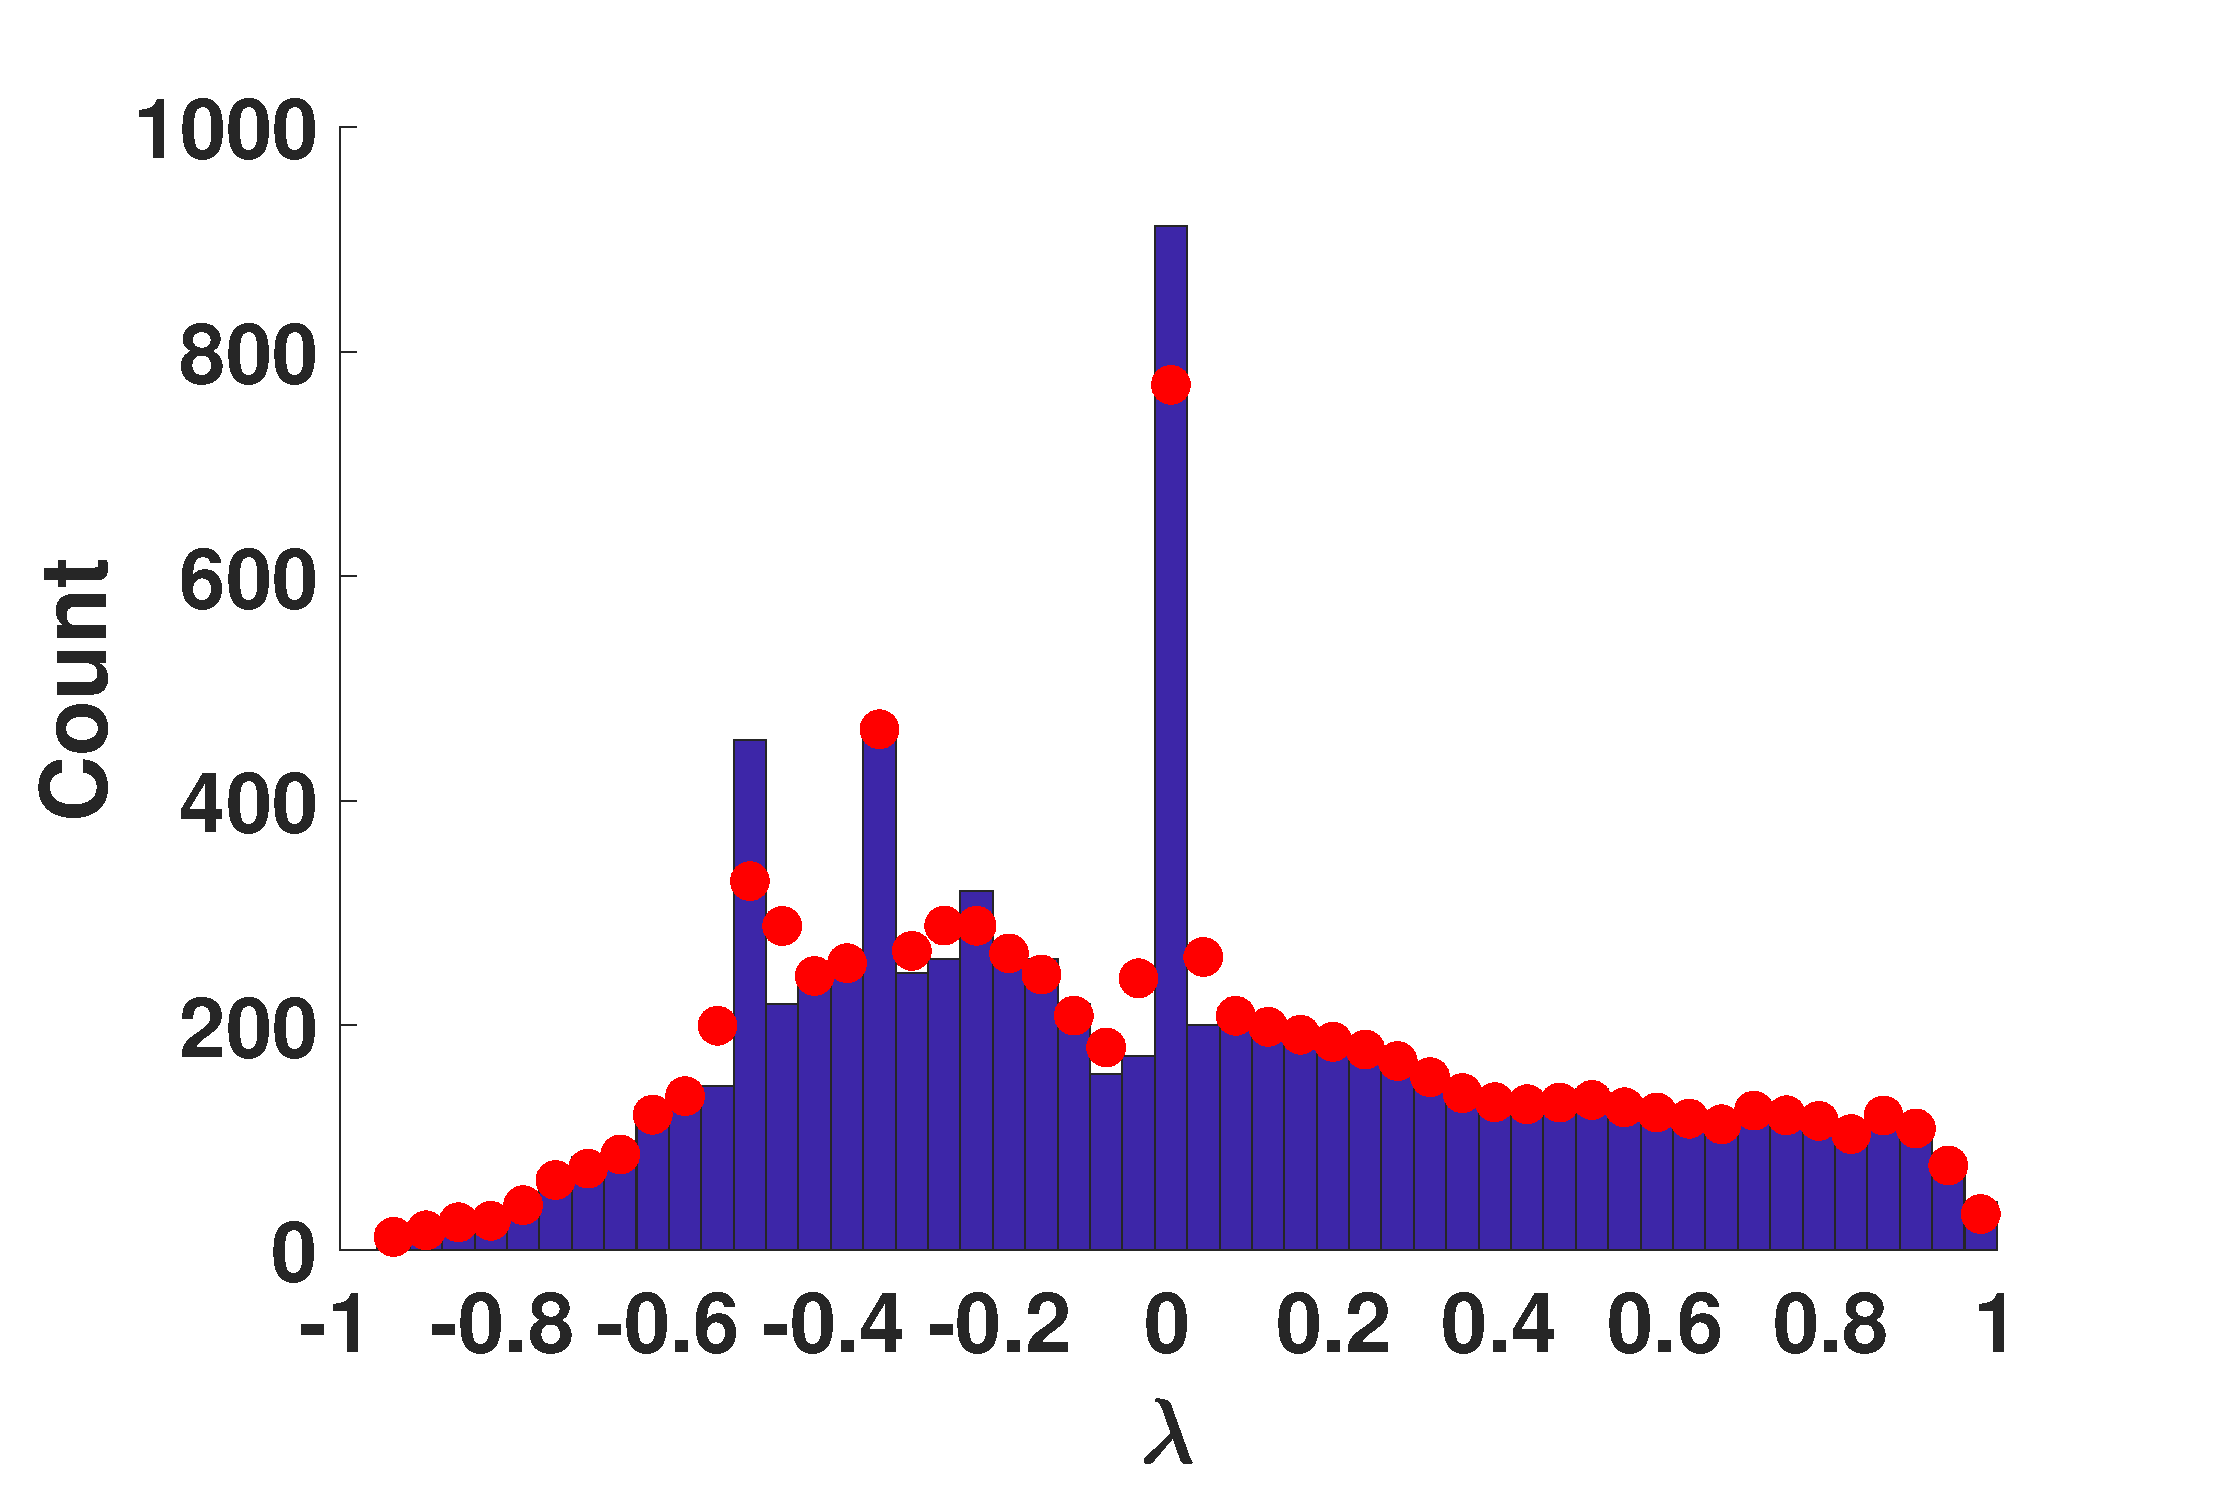
\includegraphics[width=\textwidth,trim = .3cm 0.5cm 3.2cm 1.3cm,clip]
    {./ndos/pics/hepth_twofilter}
    \caption{Filter at $\lambda=-1/3$}\label{fig:hepth_2filt}
  \end{subfigure}
  %
  \begin{subfigure}{0.47\textwidth}
    \centering
    \captionsetup{justification=centering}
    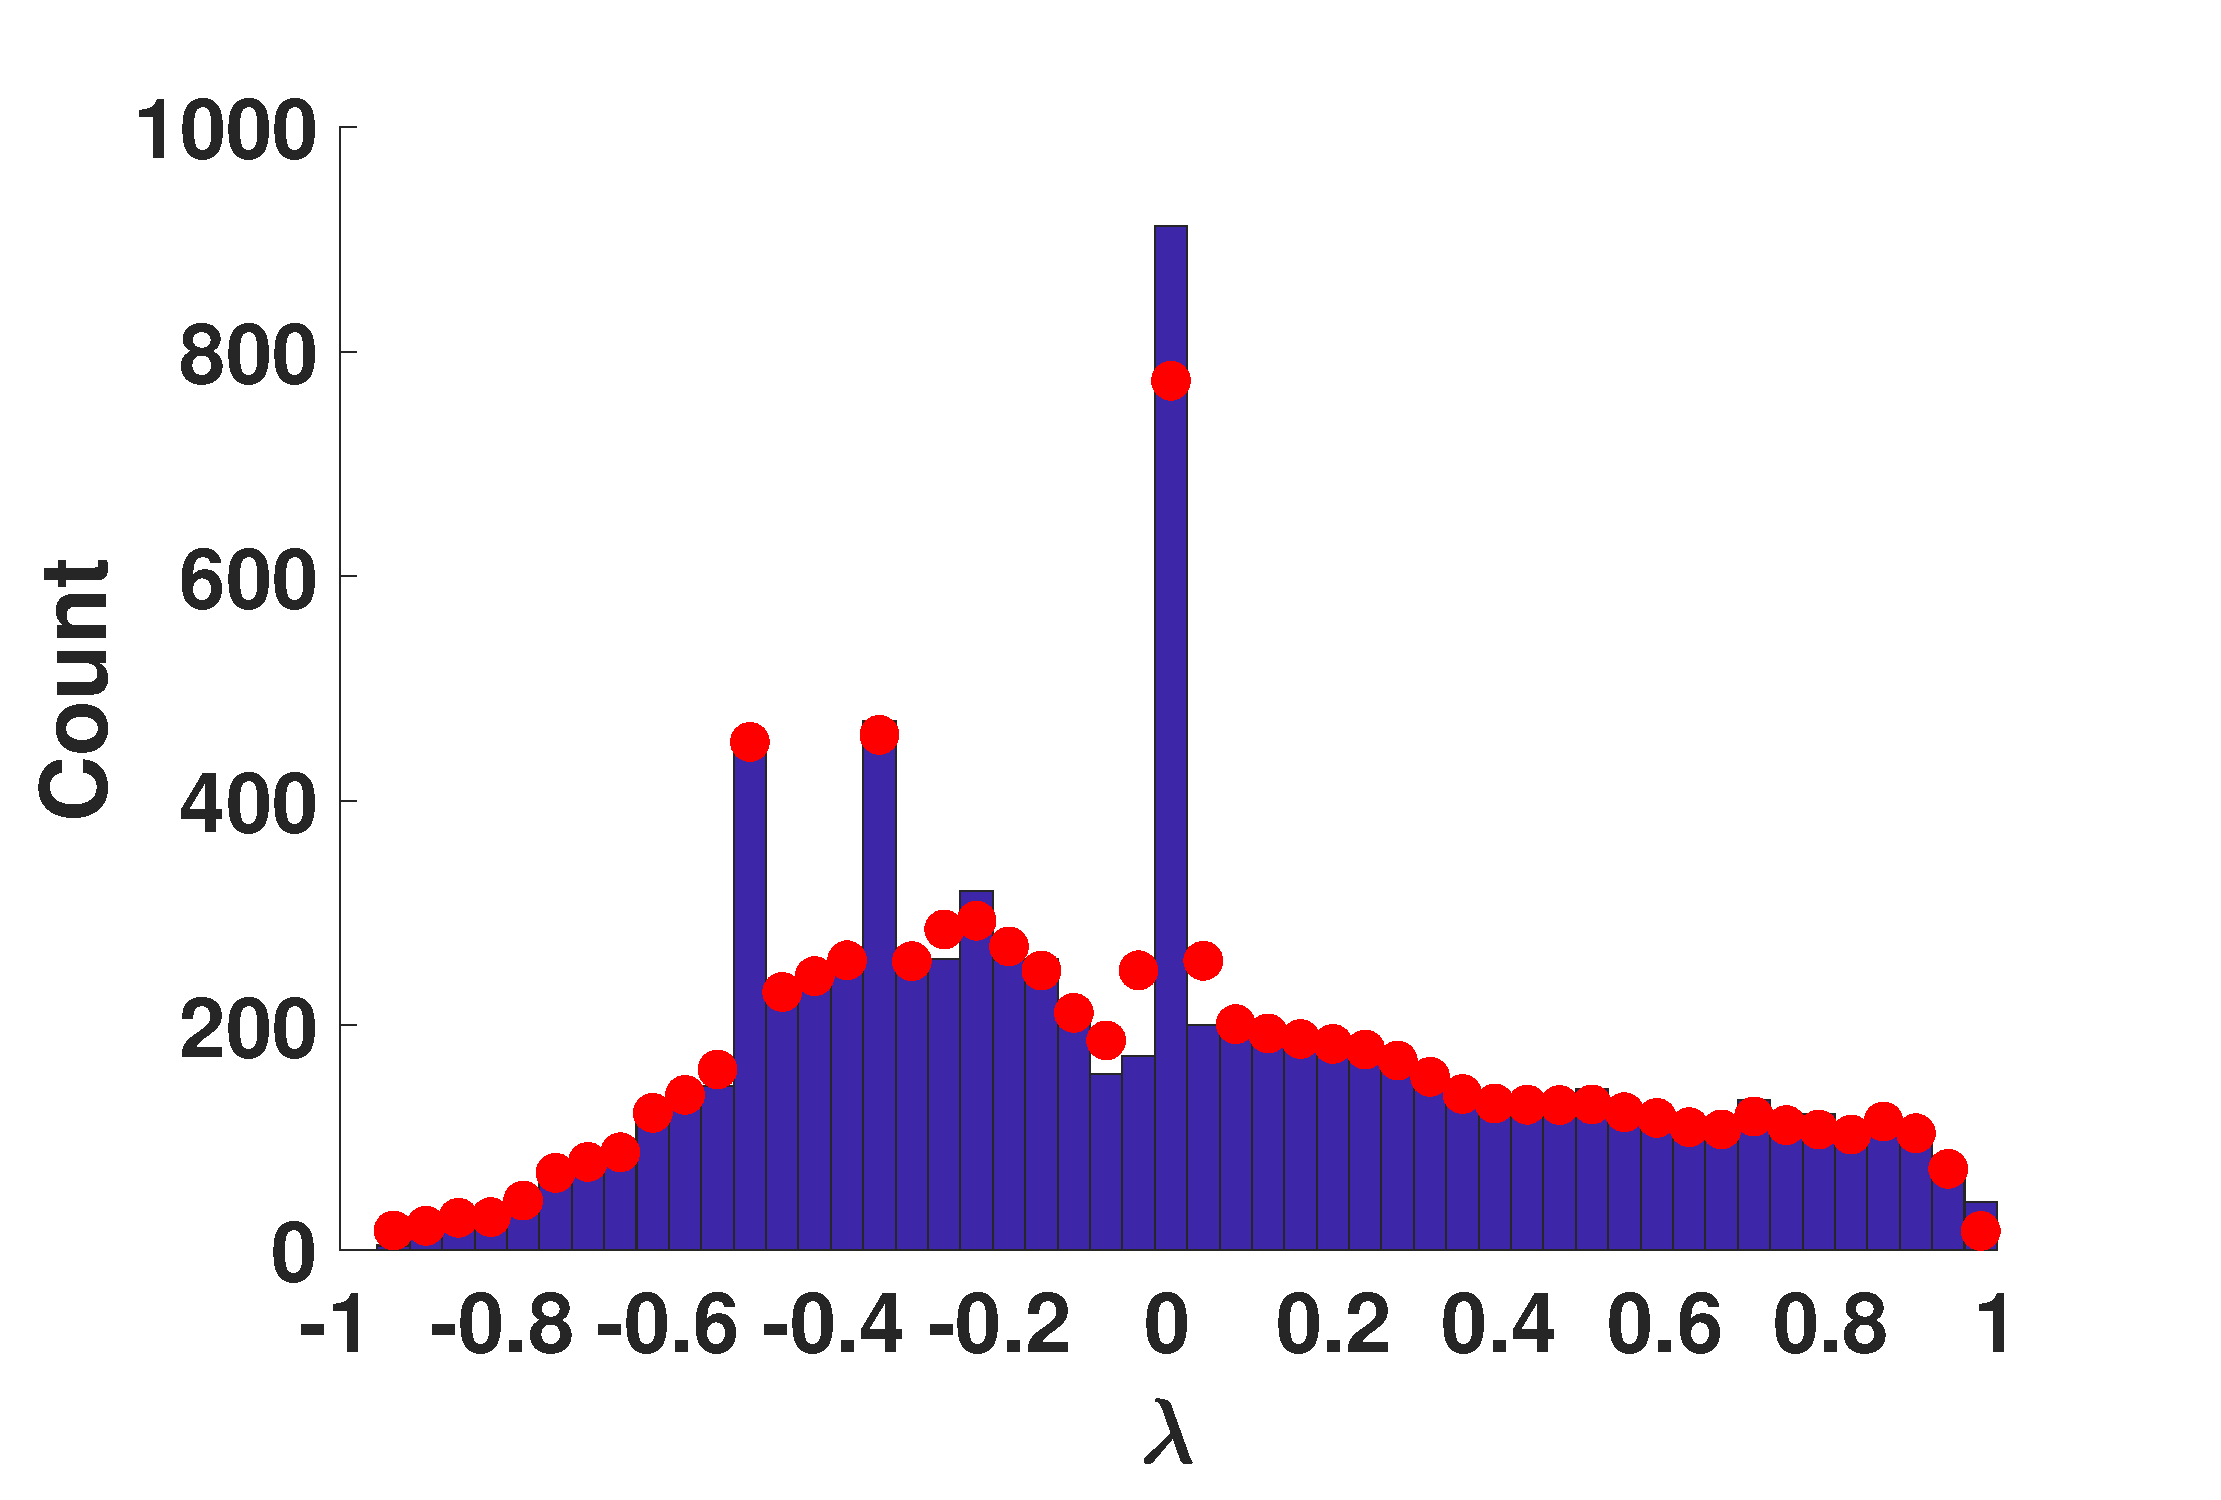
\includegraphics[width=\textwidth,trim = .3cm 0.5cm 3.2cm 1.3cm,clip]
    {./ndos/pics/hepth_threefilter}
    \caption{Filter at $\lambda=-1/2$}\label{fig:hepth_3filt}
  \end{subfigure}
  %
  \begin{subfigure}{0.47\textwidth}
    \centering
    \captionsetup{justification=centering}
    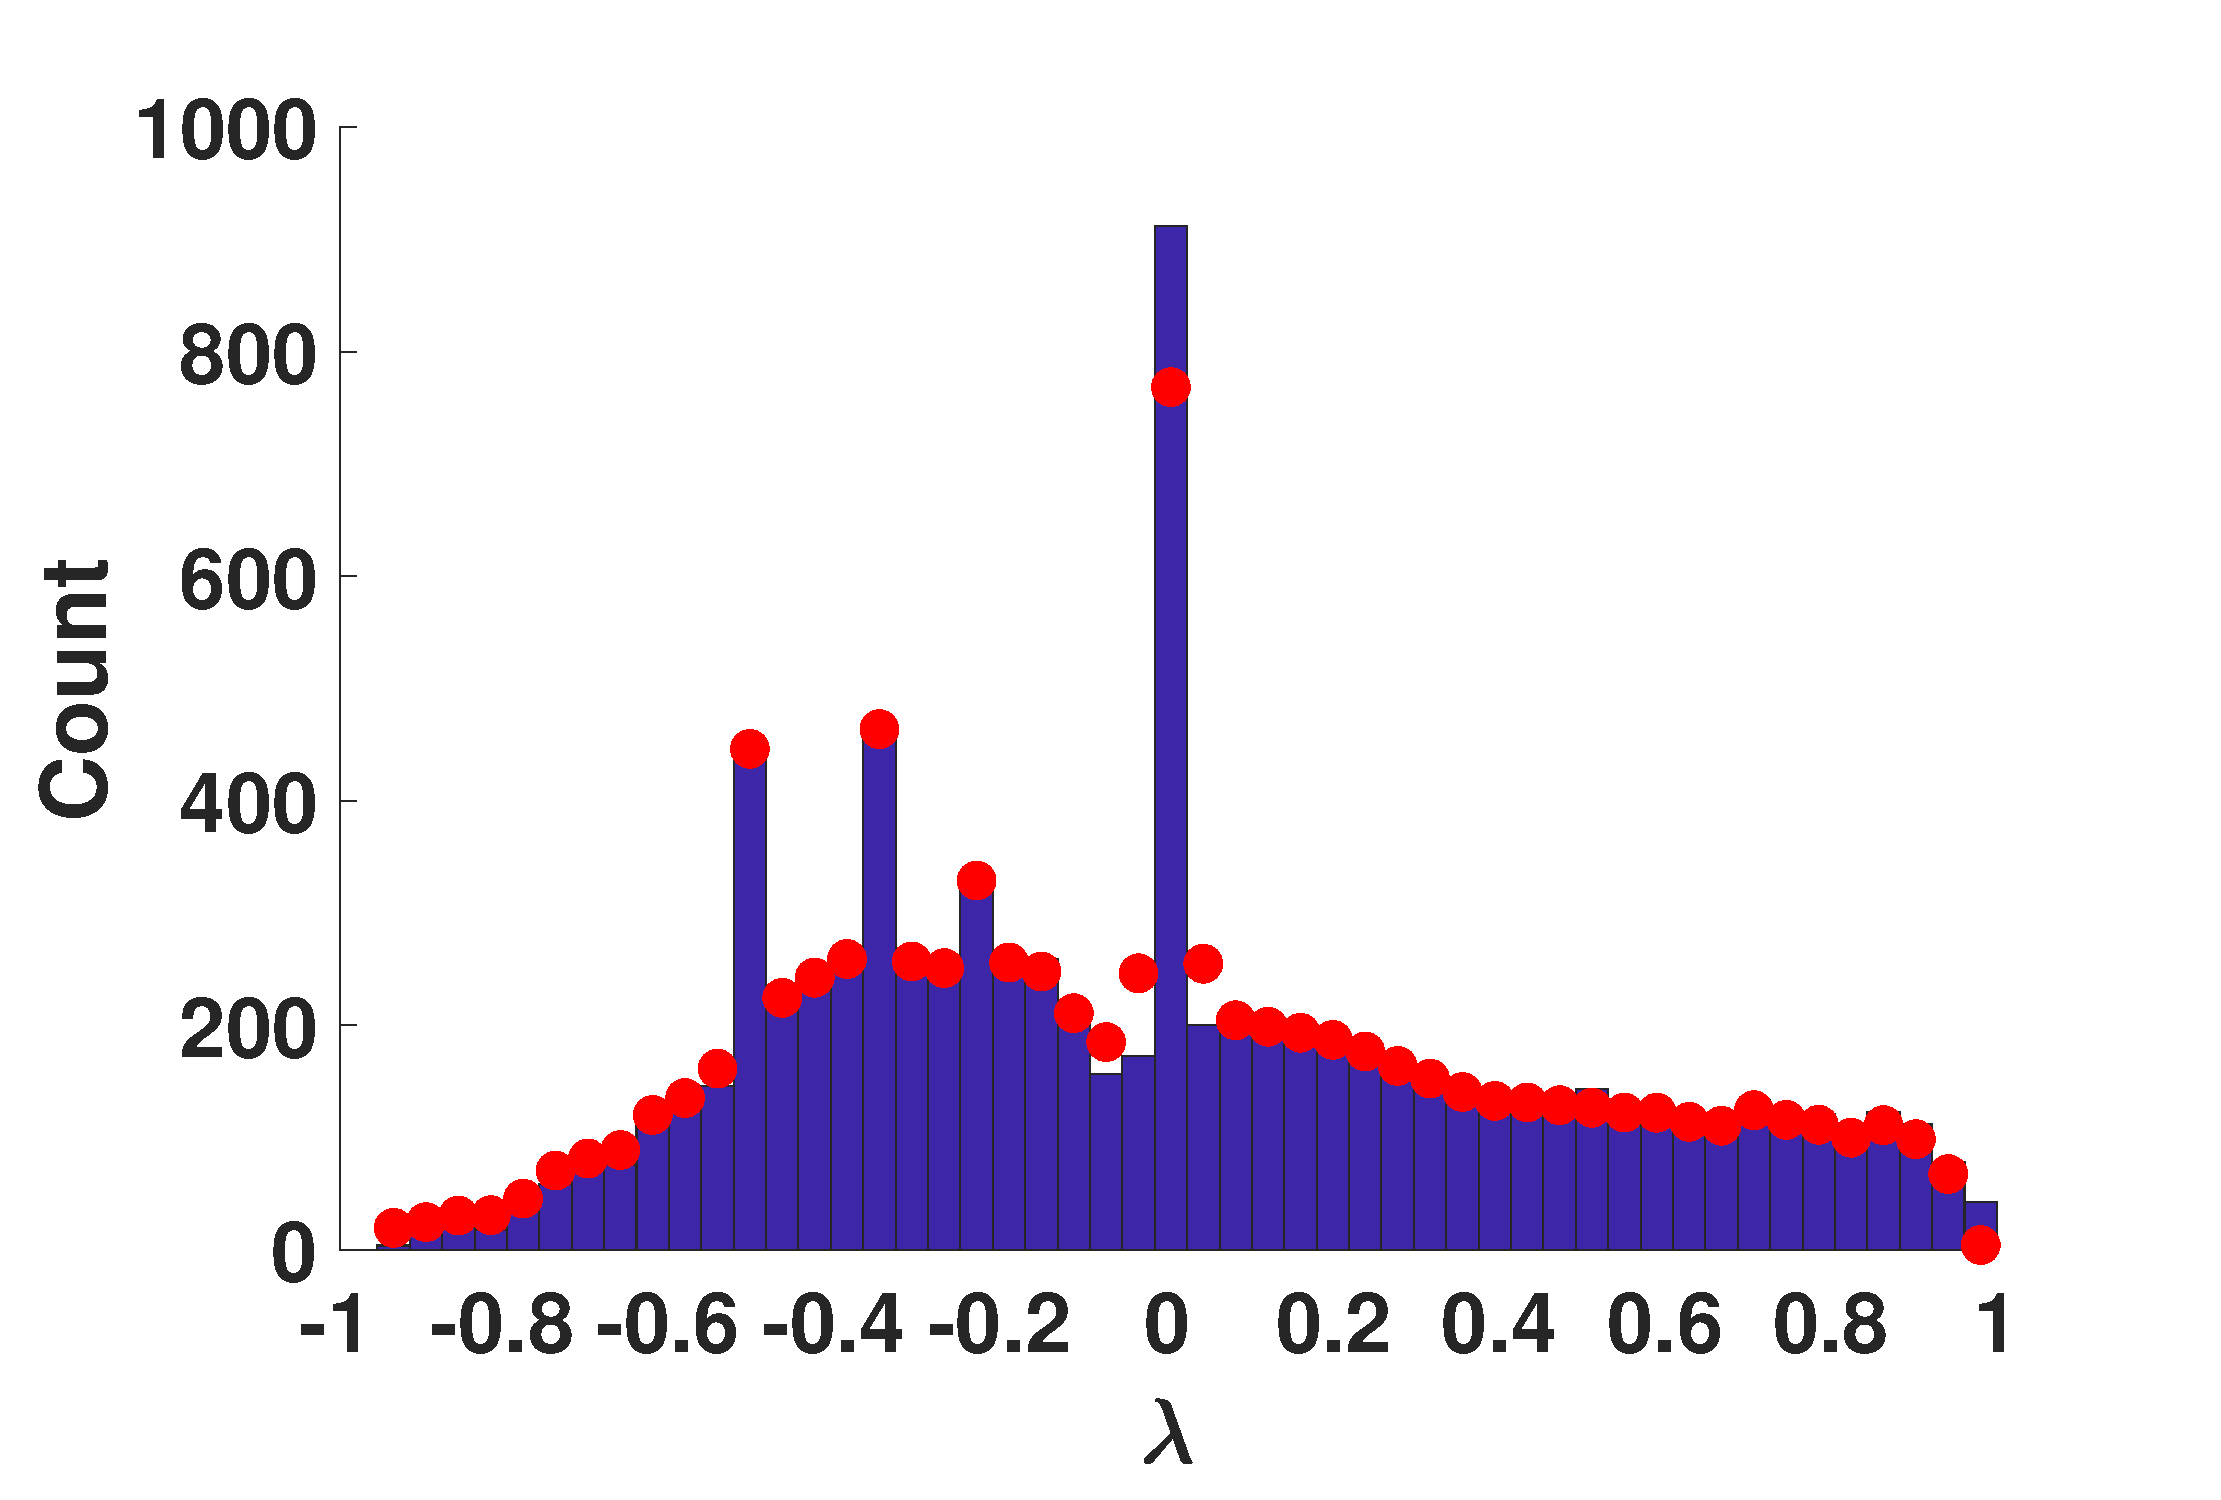
\includegraphics[width=\textwidth,trim = .3cm 0.5cm 3.2cm 1.3cm,clip]
    {./ndos/pics/hepth_fourfilter}
    \caption{Filter at $\lambda=-1/4$}\label{fig:hepth_4filt}
  \end{subfigure}
  %
  \hspace{0.8cm}
  \begin{subfigure}{0.47\textwidth}
    \centering
    \captionsetup{justification=centering}
    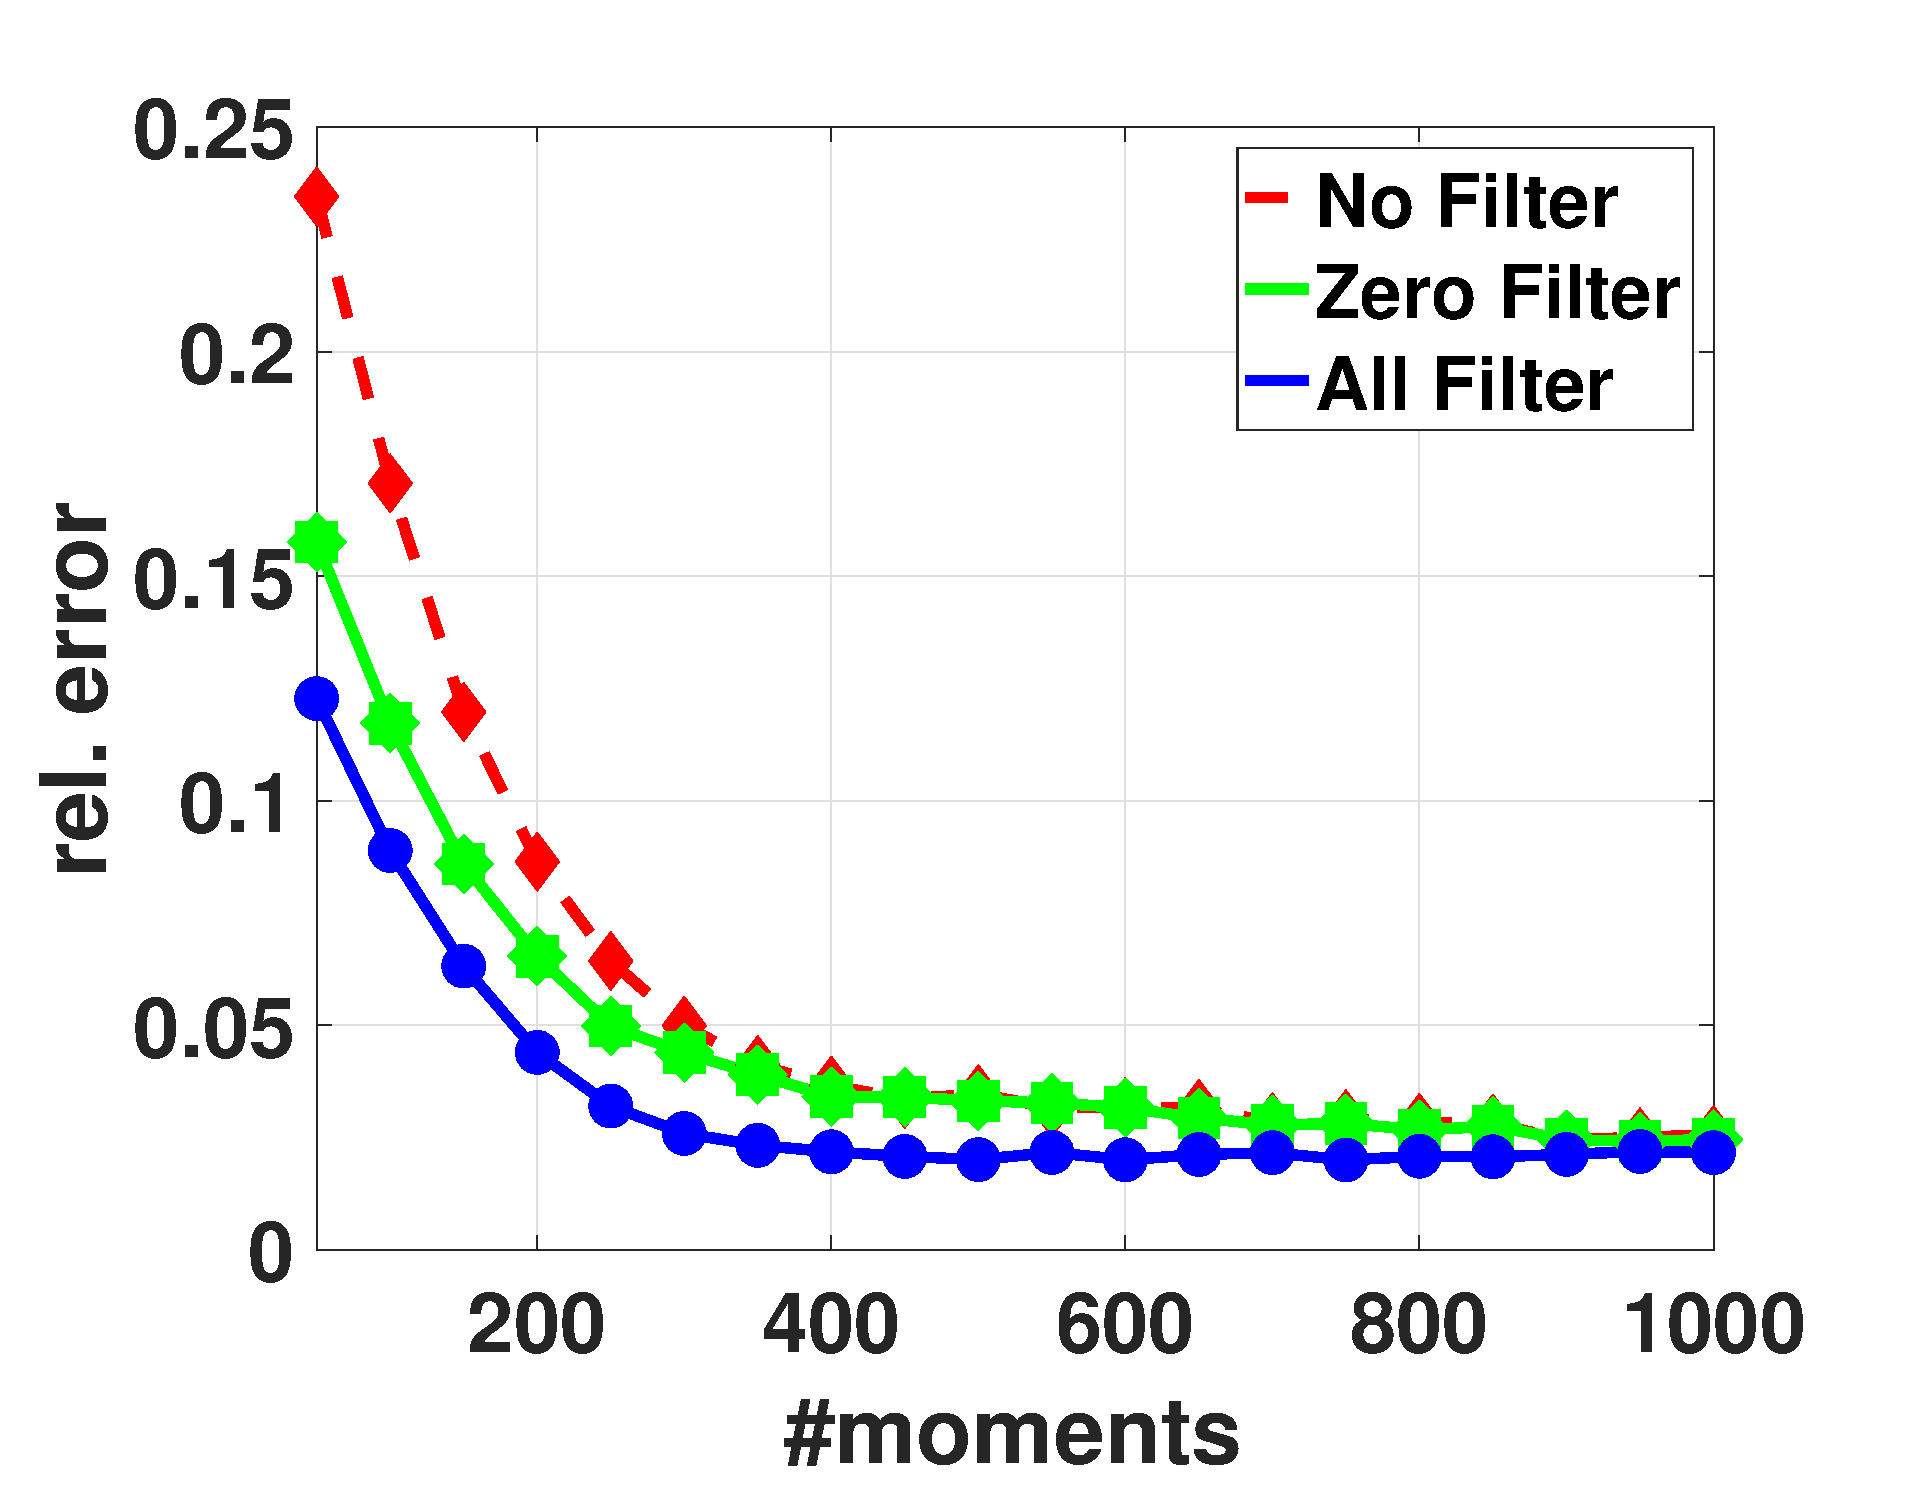
\includegraphics[width=0.9\textwidth,trim = .3cm 0cm 1.5cm 1.3cm,clip]
    {./ndos/pics/filter_error}
    \caption{Relative Error}\label{fig:hepth_error}
  \end{subfigure}
  \caption{The improvement in accuracy of the spectral histogram approximation
  on the normalized adjacency matrix for the High Energy Physics Theory (HepTh)
  Collaboration Network, as we sweep through spectrum and filter out motifs. The
  graph has $8,638$ nodes and $24,816$ edges. Blue bars are the real spectrum,
  and red points are the approximated heights. \cref{fig:hepth_0filt}-
  \ref{fig:hepth_4filt} use $100$ moments and $20$ probe vectors. \cref{fig:hepth_error} shows the relative $L_1$ error of the spectral
  histogram when using no filter, filter at $\lambda=0$, and all filters.}
  \label{fig:motif_filt}
\end{figure}

\section{Error Analysis}\label{ndossec:err}
	\subsection{KPM Approximation Error}
This section provides an error bound for our regularized DOS approximation
$K_\sigma\ast\mu$. We will start with the following theorem.
\begin{theorem}[\bf{Jackson's Theorem~\cite{jackson1911genauigkeit}}]
\label{thm:Jackson_damping}
	If $f:[-1,1]\rightarrow \BBR$ is Lipschitz continuous with constant $L$, its
	best degree $M$ polynomial approximation $\hat{f}^M$ has an $L_\infty$ 
	error of at most $6L/M$. The approximation can be constructed as
	\begin{equation}
		\hat{f}^M = \sum_{m=0}^MJ_mc_mT_m(x)\,,
	\end{equation}
	where $J_m$ are Jackson smoothing factors and $c_m$ are the Chebyshev
	coefficients.
\end{theorem}
\nomenclature[1]{$J_m$}{Jackson smoothing factors}
\nomenclature[1]{$c_m$}{Chebyshev moments}
We can pick a smooth mollifier $K$ with $\text{Lip}(K)=1$. For any $\nu\in\BBR$
and $\lambda\in [-1,1]$ there exists a degree $M$ polynomial such that 
\begin{equation}
	\abs{K_\sigma(\nu-\lambda)-\widehat{K}^{M}_\sigma(\nu-\lambda)} < \frac{6L}
	{M\sigma}\,.
\end{equation}
Define $\hat{\mu}^M = \sum_{m=0}^MJ_md_m\phi_m$ to be the truncated DOS
series,
\begin{equation}
	\int_{-1}^1 \hat{f}^M(\lambda)\mu(\lambda)d\lambda = \int_{-1}^1f
	(\lambda)\hat{\mu}^M(\lambda)d\lambda = \sum_{m=0}^MJ_mc_md_m\,.
\end{equation}
Therefore,
\begin{align*}
	\norm{K_\sigma\ast(\mu-\hat{\mu}^M)}_\infty
	=& \max_\nu\abs{\int_{-1}^1K_\sigma(\nu-\lambda)(\mu(\lambda)-\hat{\mu}^M 
	(\lambda))d\lambda}\\
	\leq& \max_\nu\int_{-1}^1\abs{K_\sigma(\nu-\lambda)-\widehat{K}^M_\sigma
	(\nu-\lambda)}\mu(\lambda)d\lambda \\
	\leq& \frac{6L}{M\sigma}\,.
\end{align*}
Consider $\tilde{\mu}^M$ to be the degree $M$ approximation from KPM,
\begin{equation}
	\norm{K_\sigma\ast(\mu-\tilde{\mu}^M)}_\infty \leq \norm{K_\sigma\ast(\mu- 
	\hat{\mu}^M)}_\infty+ \norm{K_\sigma}_\infty\norm{\,\hat{\mu}^M - 
	\tilde{\mu}^M}_1\,.
\end{equation}
If we use a probe $z$ with independent standard normal entries for the
trace estimation,
\begin{equation}
	\tilde{\mu}(\lambda) = \sum_{i=1}^Nw_i^2\delta(\lambda-\lambda_i)
\end{equation}
where $w=Q^Tz$ is the weight for $z$ in the eigenbasis. Hence
\begin{equation}
	\norm{\hat{\mu}^M-\tilde{\mu}^M}_1 \leq \sum_{i=1}^N \abs{1-w_i^2}\,.
\end{equation}
Finally,
\begin{equation}
	\BBE\left[\norm{K_\sigma\ast(\mu-\tilde{\mu}^M)}\right]\leq \frac{1}
	{\sigma}\left(\frac{6L}{M}+\norm{K}_\infty\BBE\left[
	\abs{1-w_1^2}\right]\right)\,.
\end{equation}
If we take $N_z$ independent probe vectors, then $N_zw_1^2\sim\chi^2(N_z)$,
which means the expectation decays asymptotically like $\sqrt{2 / (\pi N_z)}$.

\subsection{Perturbation Analysis}
In this section, we limit our attention to symmetric graph matrix $H$.
Extracting graph information using DOS, whether as a distribution for functions
on a graph or as a direct feature in the form of spectral moments, requires
stability under small perturbations. In the case of removing/adding a few 
number of nodes/edges, the Cauchy Interlacing Theorem~\cite{magnus1988matrix}
gives a bound on each individual new eigenvalue by the old ones. For example, 
if we remove $r\ll N$ nodes to get a new graph matrix $
\widetilde{H}$, then
\begin{equation}\label{eqn:interlacing}
	\lambda_i(H)\leq \lambda_i(\widetilde{H})\leq \lambda_{i+r}(H)\quad\text{for
	}\quad i\leq N-r\,.
\end{equation}
However, this bound may not be helpful when the impact of the change is not
reflected by its size. Hence, we provide a theorem that relates the Wasserstein
distance (see \cref{eqn:waisserstein}) change and the Frobenius norm of
the perturbation. Without loss of generality, we assume the eigenvalues of $H$
lie in $[-1,1]$ already.

\begin{theorem}
	Suppose $\widetilde{H} = H + \delta H$ is the perturbed graph matrix with
	spectral density $\tilde{\mu}$, then
	\begin{equation*}
		W_1(\mu, \tilde{\mu}) \leq \norm{\delta H}_F
	\end{equation*}
\end{theorem}
\begin{proof}
	Let $\calL$ be the space of Lipschitz functions with $f(0)=0$.
	\begin{align*}\label{eqn:proof1}
		W_1(\mu, \tilde{\mu})=& \sup_{f\in\calL, \Lip(f)=1} \int f(\lambda) (\mu
		(\lambda)-\tilde{\mu}(\lambda))d\lambda \\
		=&\frac{1}{N}\sup_{f\in\calL, \Lip(f)=1}\tr(f(H)-f(\widetilde{H}))\\
		\leq& \sup_{f\in\calL, \Lip(f)=1, \|v\|=1} v^T(f(H)-f(\widetilde{H}))v\,.
	\end{align*}
	By Theorem 3.8 from Higham~\cite{higham2008functions}, the perturbation on
	$f(H)$ is bounded by the Fr\'{e}chet derivative,
	\begin{equation}
		\norm{f(H) - f(\widetilde{H})}_2\leq \Lip(f)\|\delta H\|_F + \calo(\|\delta
		H\|_F).
	\end{equation}
\end{proof}

\section{Experiments}\label{ndossec:exp}
	\subsection{Gallery of DOS/PDOS}
We first present our spectral histogram approximation from DOS/ PDOS on a wide
variety of graphs, including collaboration networks, online social networks,
road networks and autonomous systems (dataset details are in the appendix). For
all examples, we apply our methods to the normalized adjacency matrices using
$500$ Chebyshev moments and $20$ Hadamard probe vectors. Afterwards, the
spectral density is integrated into $50$ histogram bins. In \cref{fig:gallery},
the DOS approximation is on the first row, and the PDOS approximation is on the
second. When a spike exists in the spectrum, we apply motif filtering, and DOS
is zoomed appropriately to show the remaining part. For PDOS, we stack the
spectral histograms for all nodes vertically, sorted by their projected weights
on the leading left singular vector. Red indicates that a node has high weight
at certain parts of the spectrum, whereas blue indicates low weight.

We observe many distinct shapes of spectrum in our examples. The eigenvalues of
denser graphs, such as the Marvel characters network (\ref{fig:marvel_ldos}:
average degree $52.16$) and Facebook union of ego networks 
(\ref{fig:facebook_ldos}: average degree $43.69$), exhibit decay similar to
thepower-law around $\lambda=0$. There has been study on the power-law
distribution in the eigenvalues of the adjacency and the Laplacian matrix, but
it only focuses on the leading eigenvalues rather than the entire spectrum~
\cite{eikmeier2017revisiting} for large real-world datasets. Relatively sparse
graphs (\ref{fig:erdos_ldos}: average degree $3.06$,; \ref{fig:as_ldos}: average
degree $4.13$) often possess spikes, especially around $\lambda=0$, which
reflect a larger set of loosely-connected boundary nodes. It is much more
evident in the PDOS spectral histograms, which allow us to pick out the nodes
with dominant weights at $\lambda=0$ and those that contribute most to local
structures. Finally, though the road network is quite sparse (ave. deg $2.50$),
its regularity results in a lack of special features, and most nodes contribute
evenly to the spectrum according to PDOS.

\begin{figure}[htp]
  \begin{subfigure}[t]{0.19\textwidth}
    \centering  
    \captionsetup{justification=centering,font=scriptsize}
    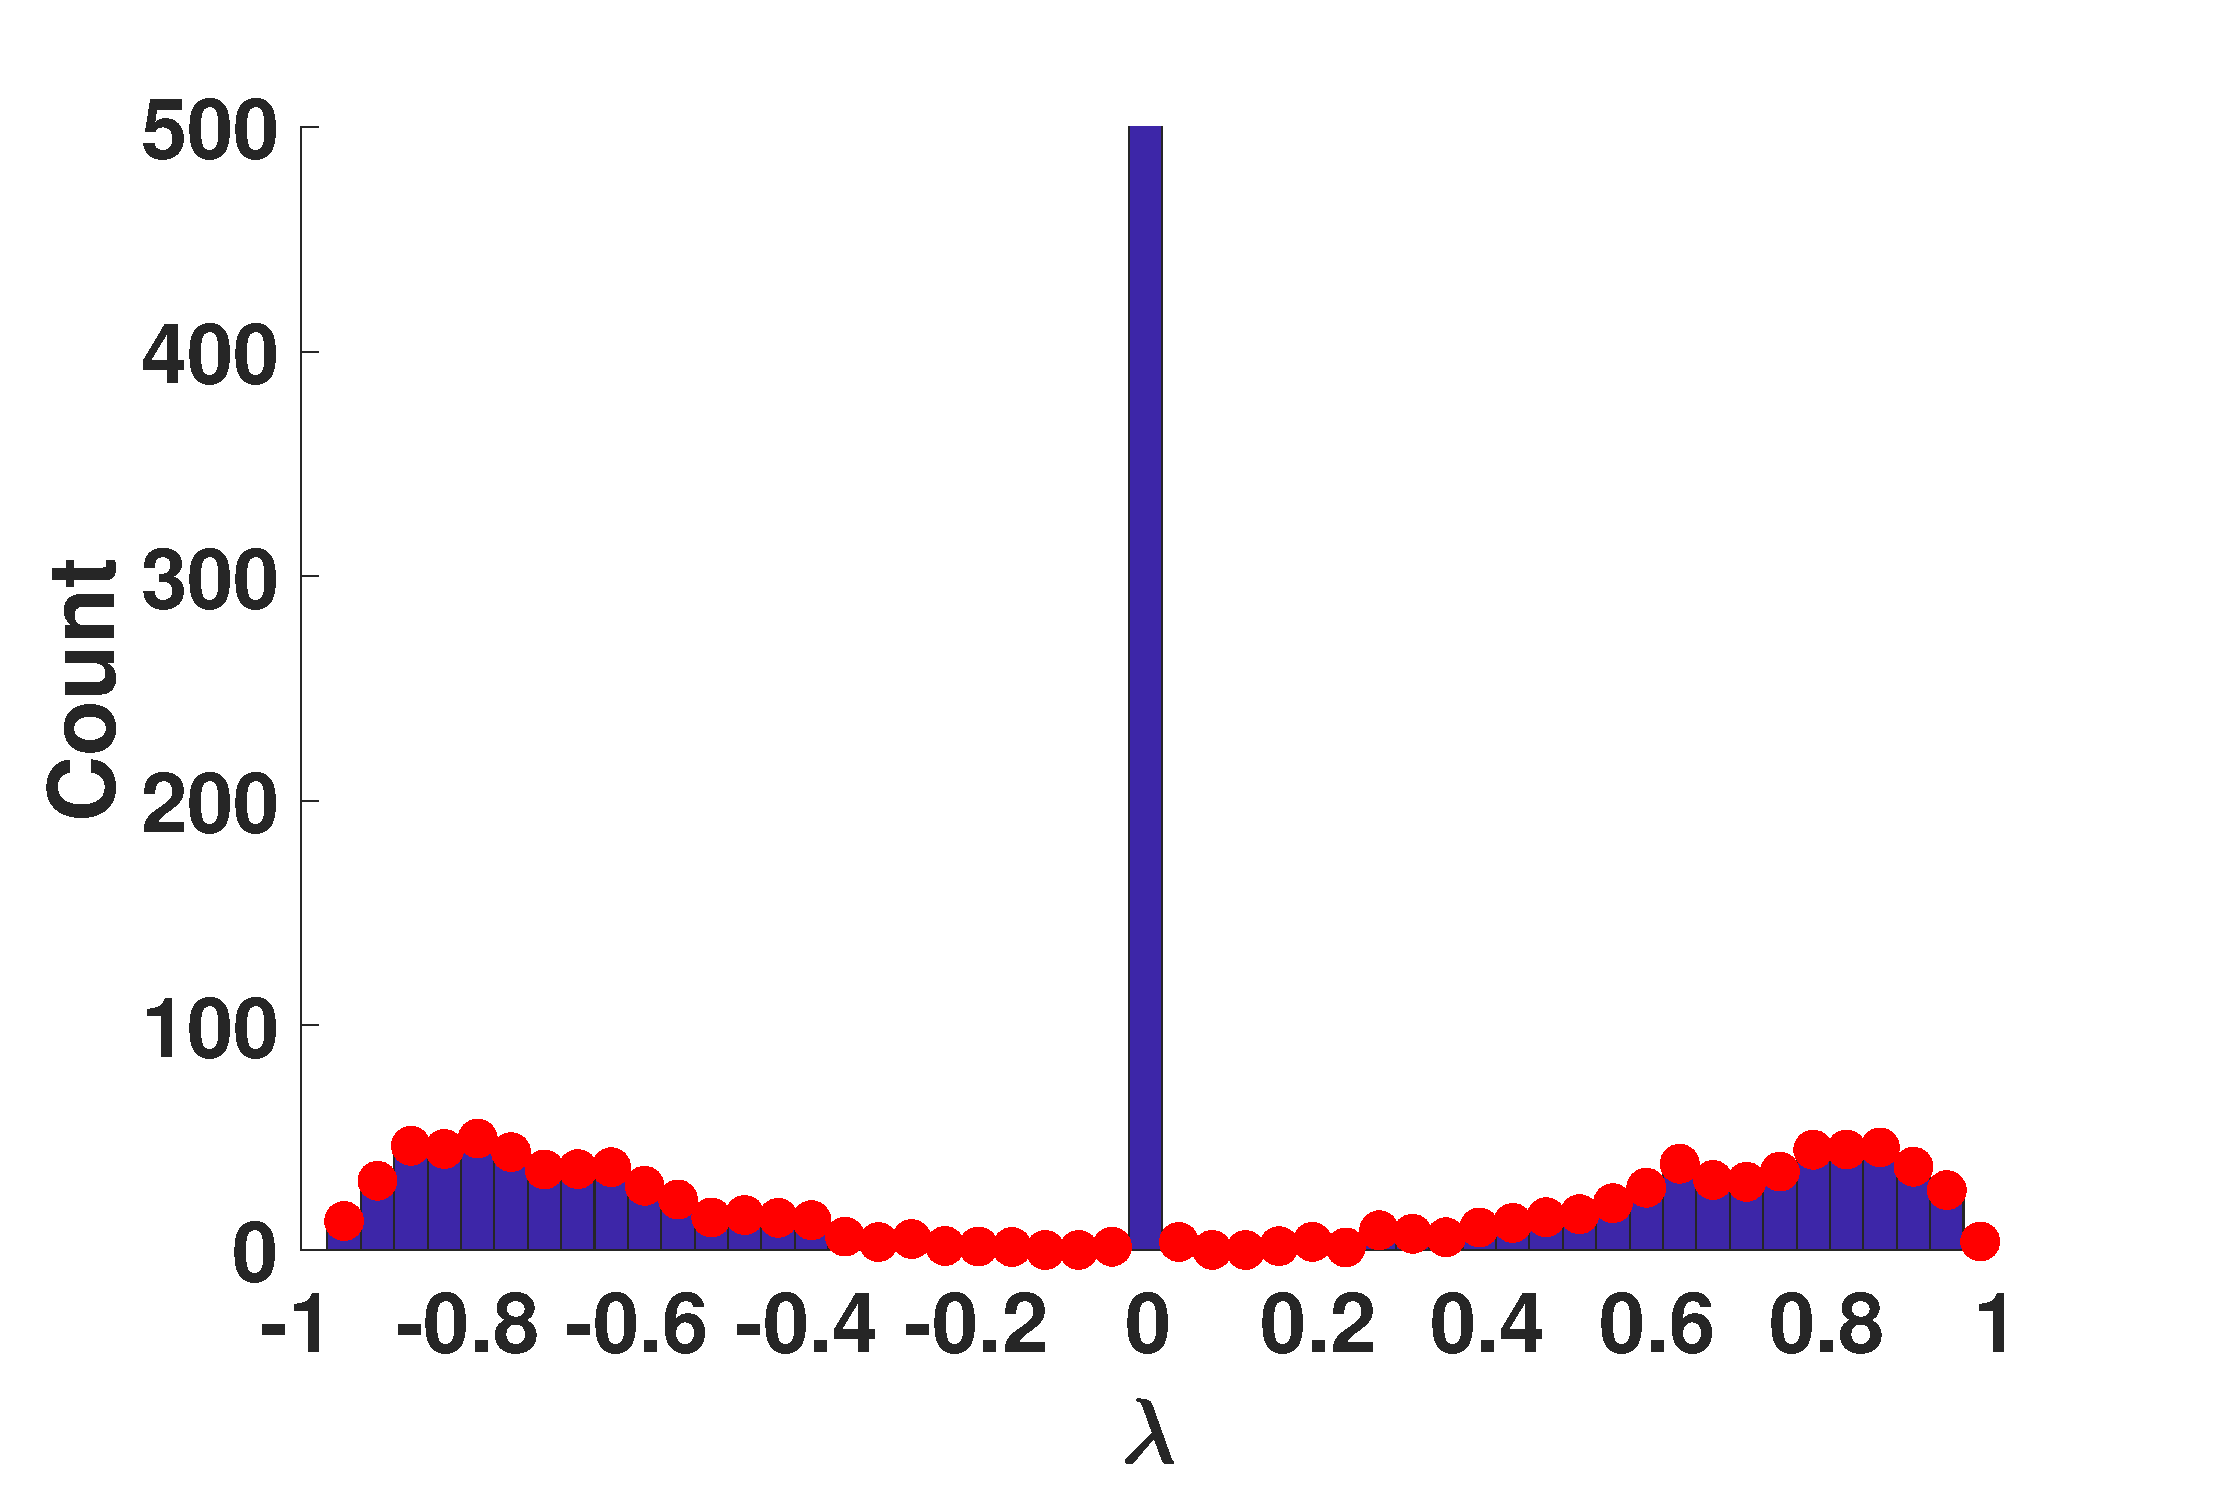
\includegraphics[width=\textwidth,trim = .4cm 0.5cm 3.5cm 1.3cm,clip]
    {./ndos/pics/erdos}
    \label{fig:erdos_dos}
  \end{subfigure}
  %
  \begin{subfigure}[t]{0.19\textwidth}
    \centering  
    \captionsetup{justification=centering,font=scriptsize}
    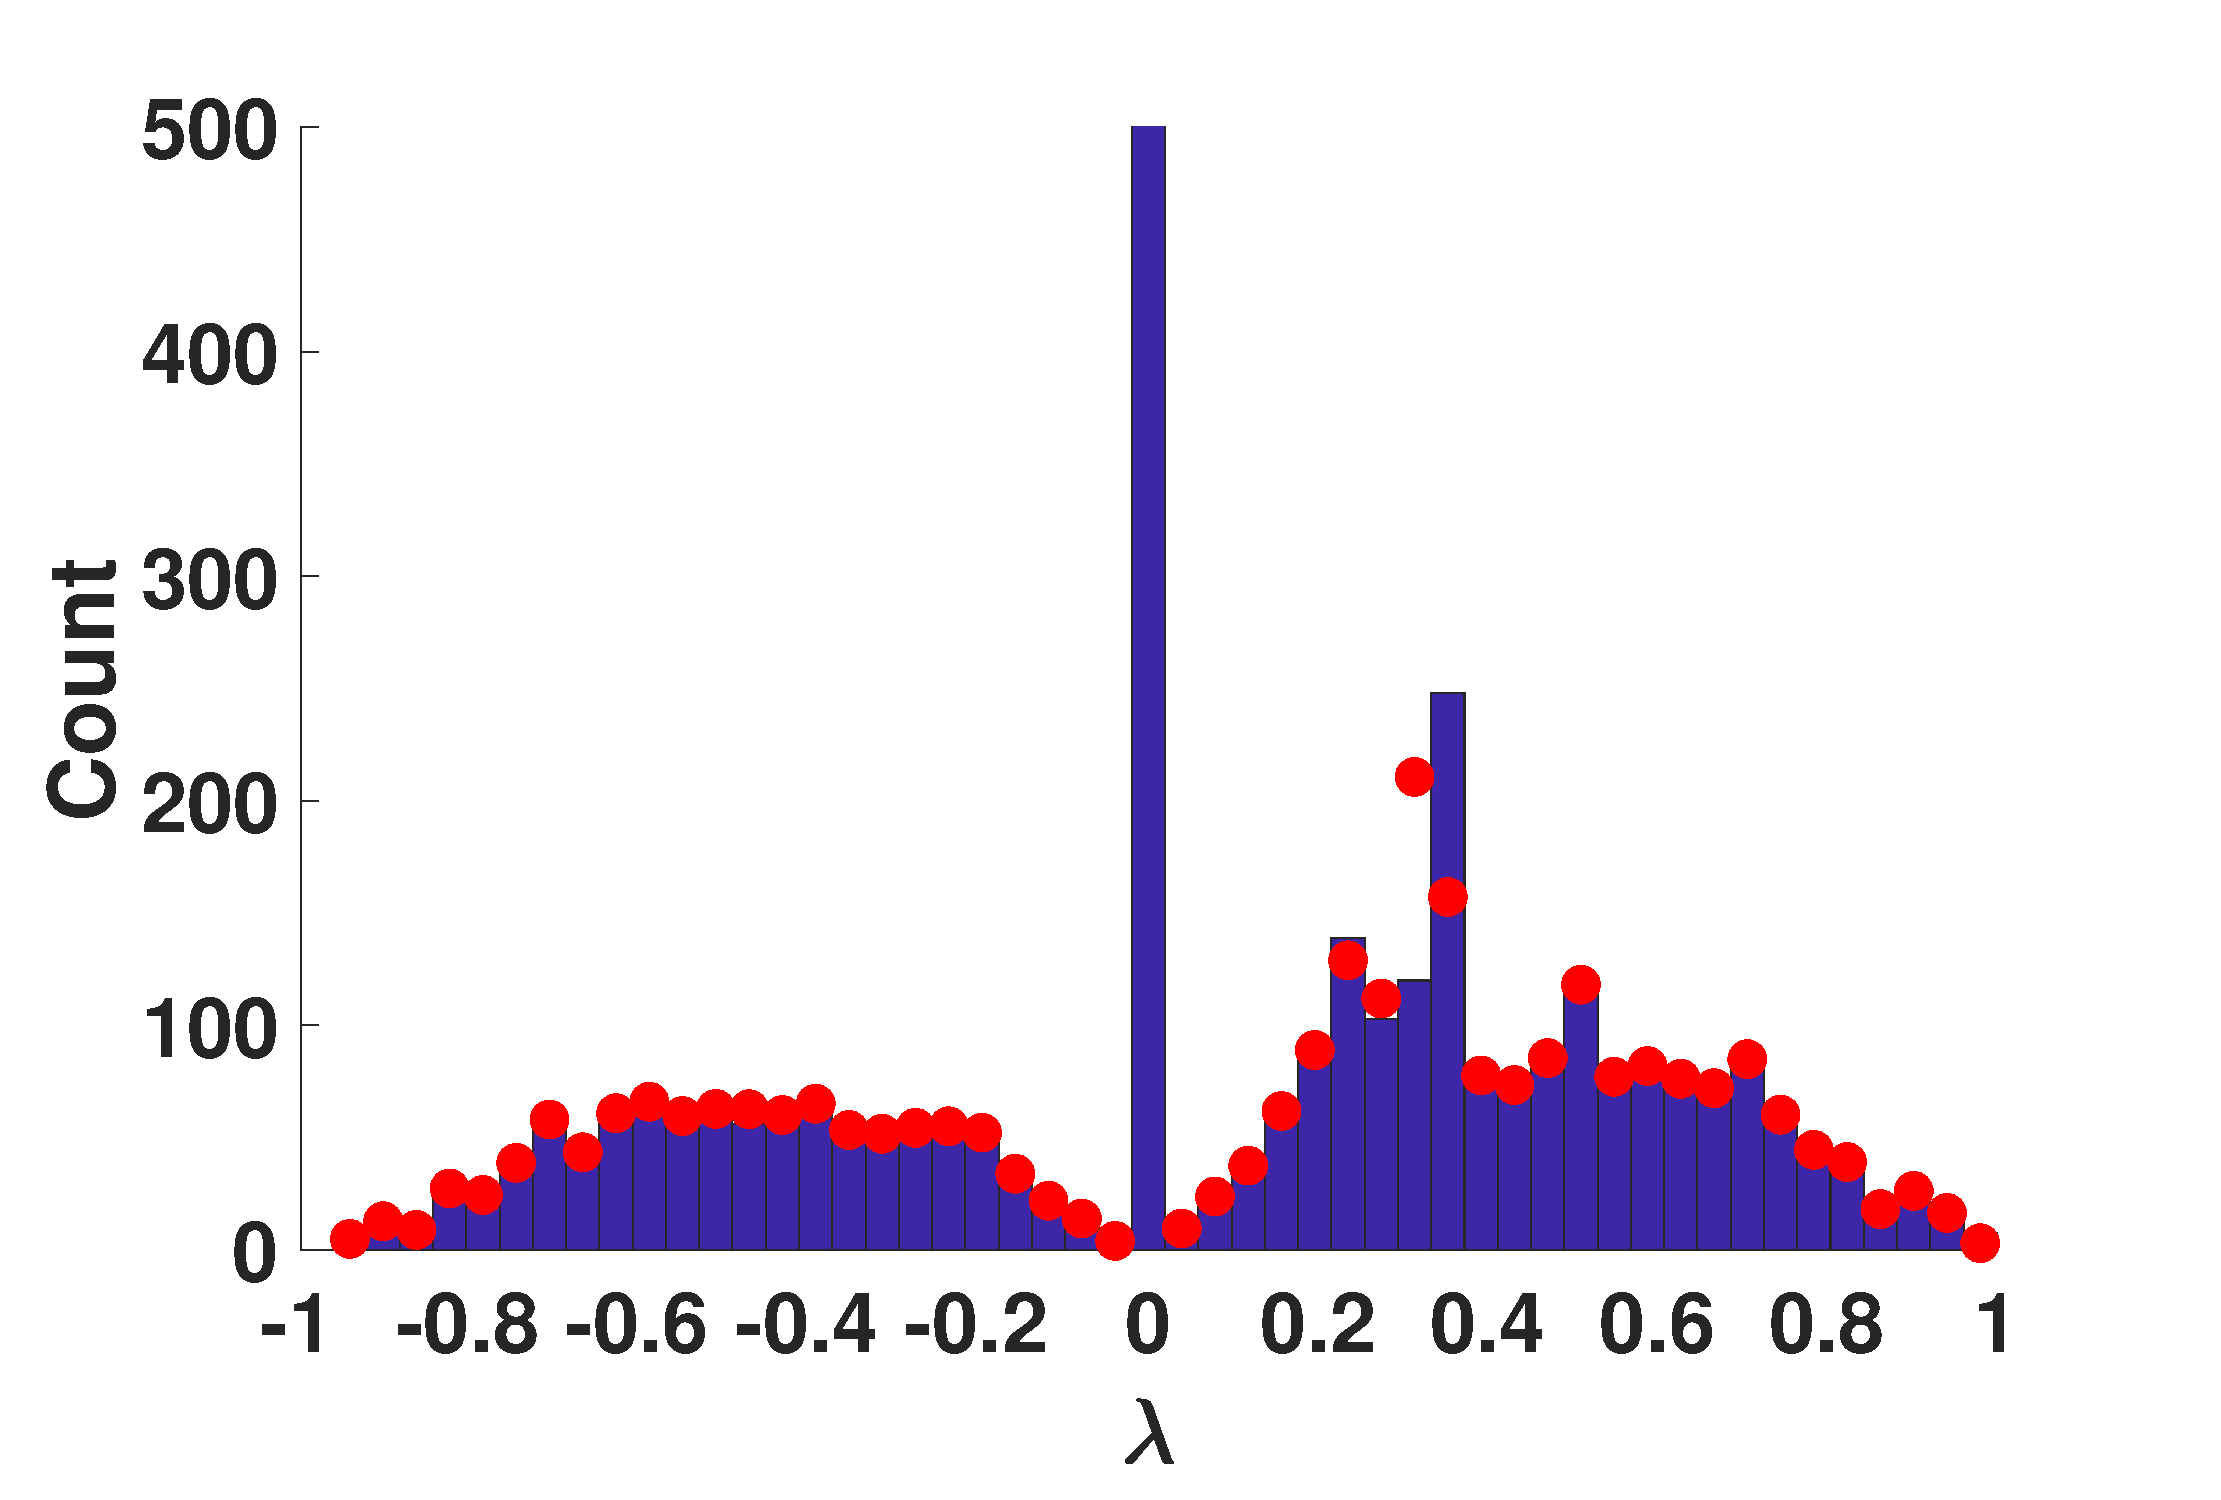
\includegraphics[width=\textwidth,trim = .4cm 0.5cm 3.5cm 1.3cm,clip]
    {./ndos/pics/as19991115}
    \label{fig:as_dos}
  \end{subfigure}
  %
  \begin{subfigure}[t]{0.19\textwidth}
    \centering
    \captionsetup{justification=centering,font=scriptsize}
    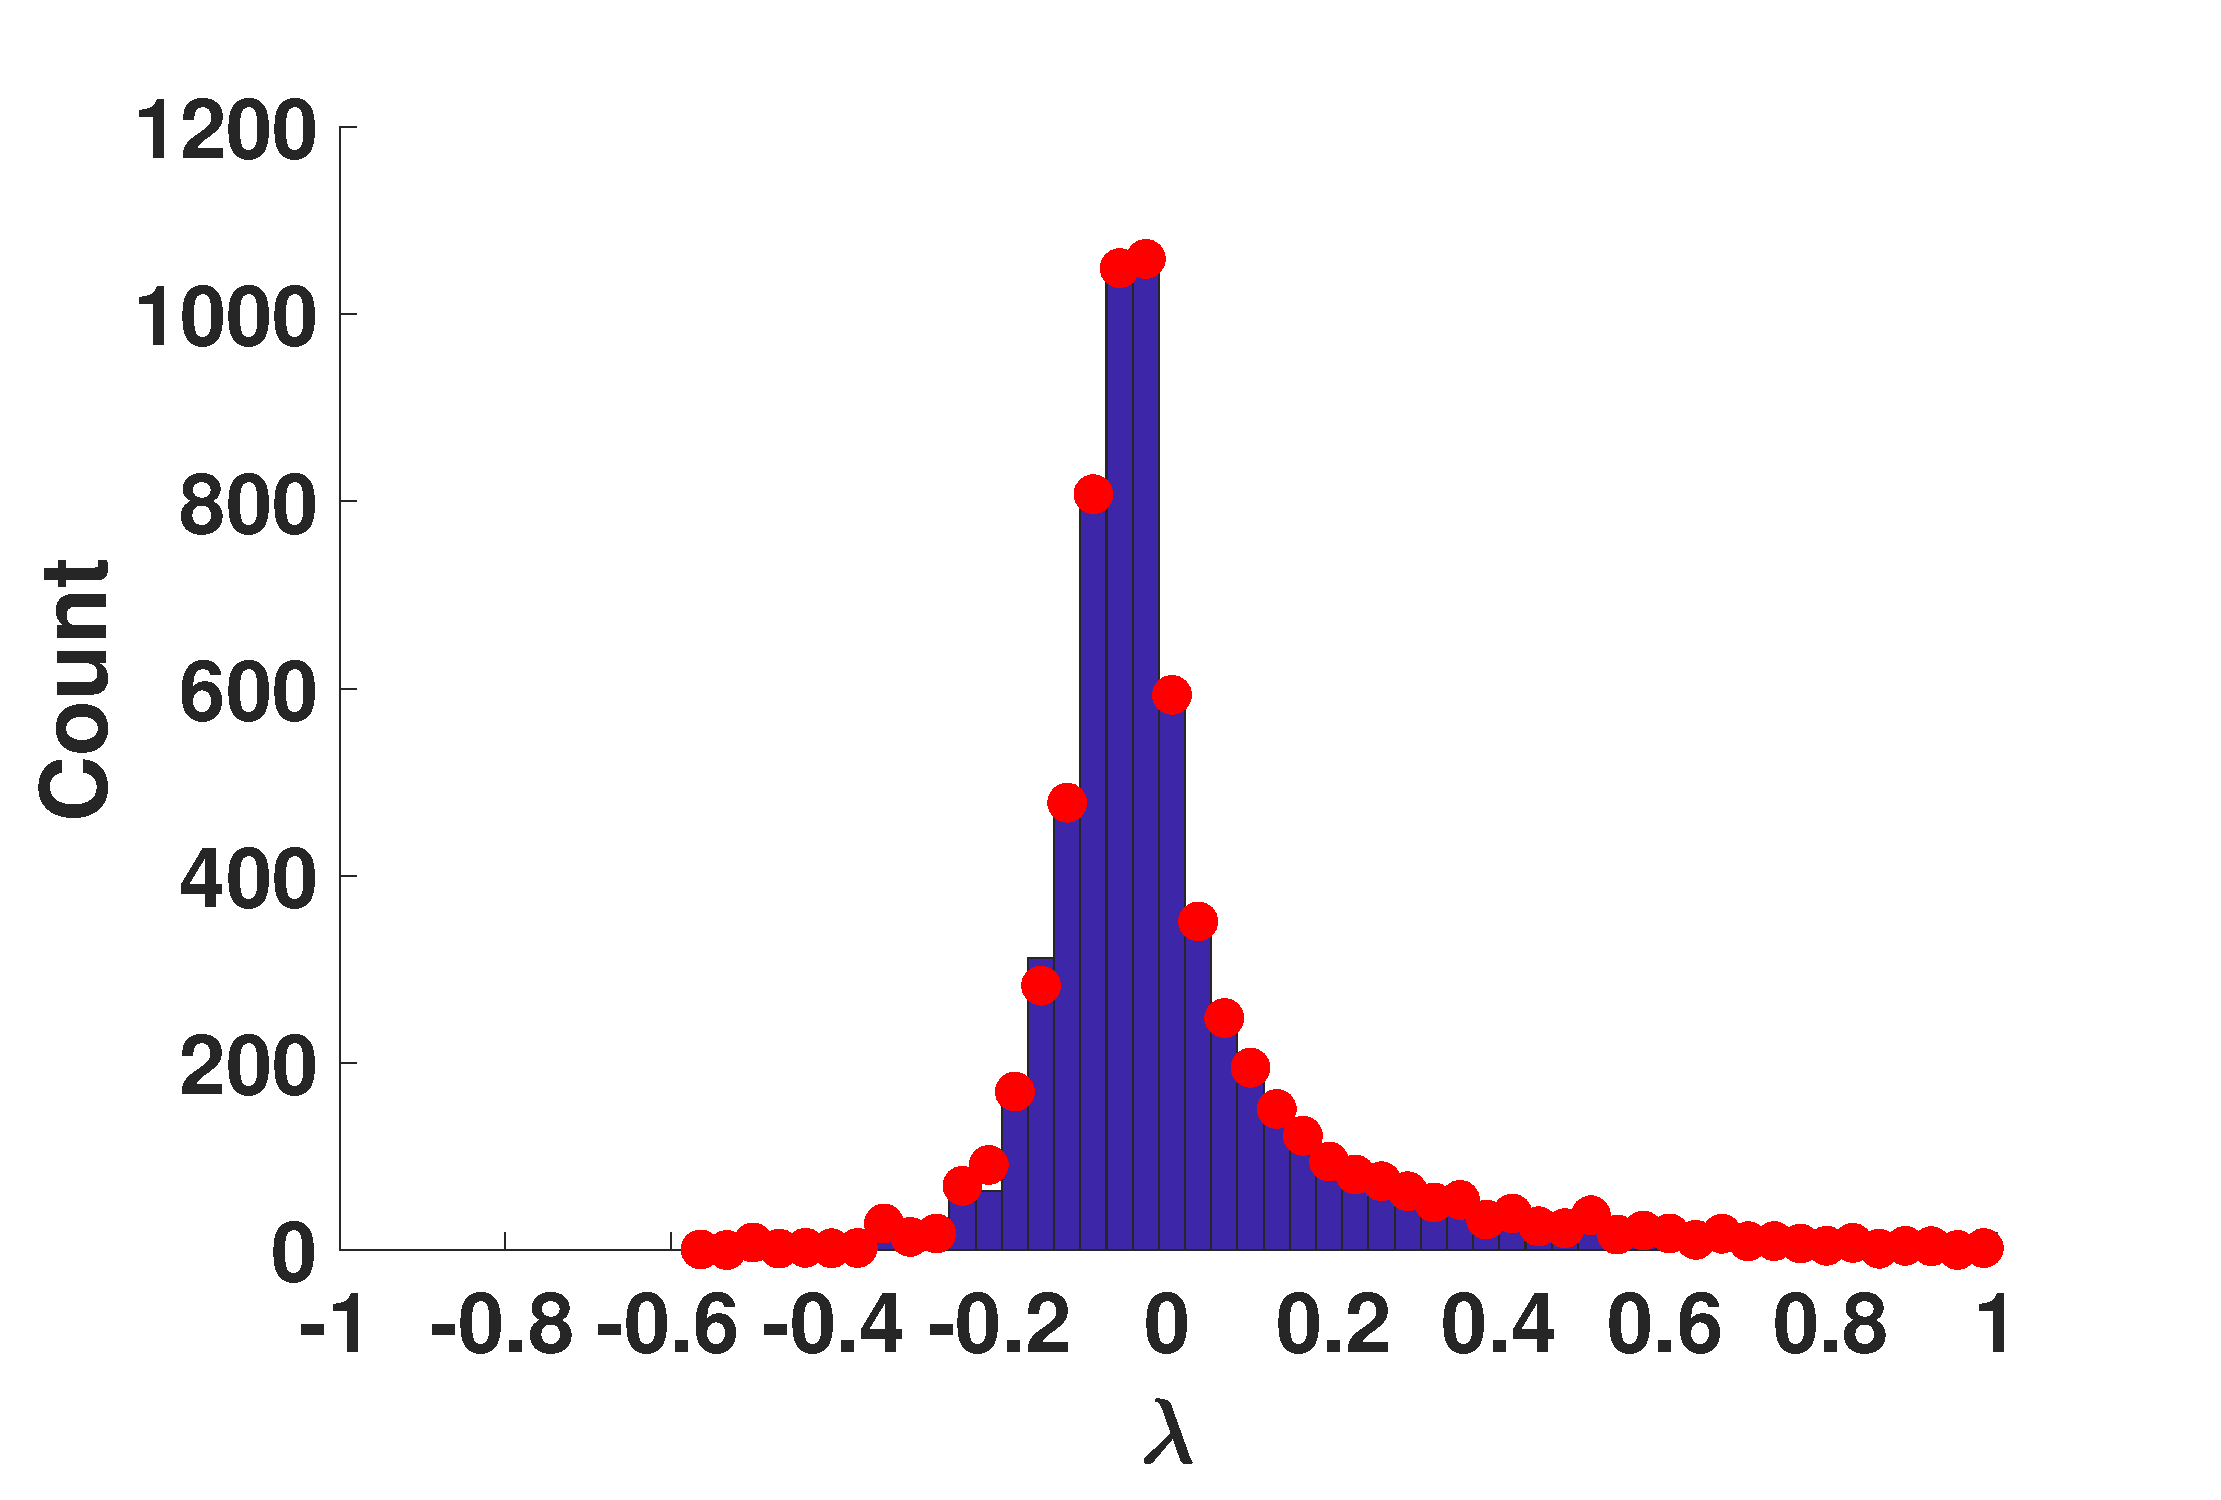
\includegraphics[width=\textwidth,trim = .4cm 0.5cm 3.5cm 1.3cm,clip]
    {./ndos/pics/marvel}
    \label{fig:marvel_dos}
  \end{subfigure}
  \begin{subfigure}[t]{0.19\textwidth}
    \centering  
    \captionsetup{justification=centering,font=scriptsize}
    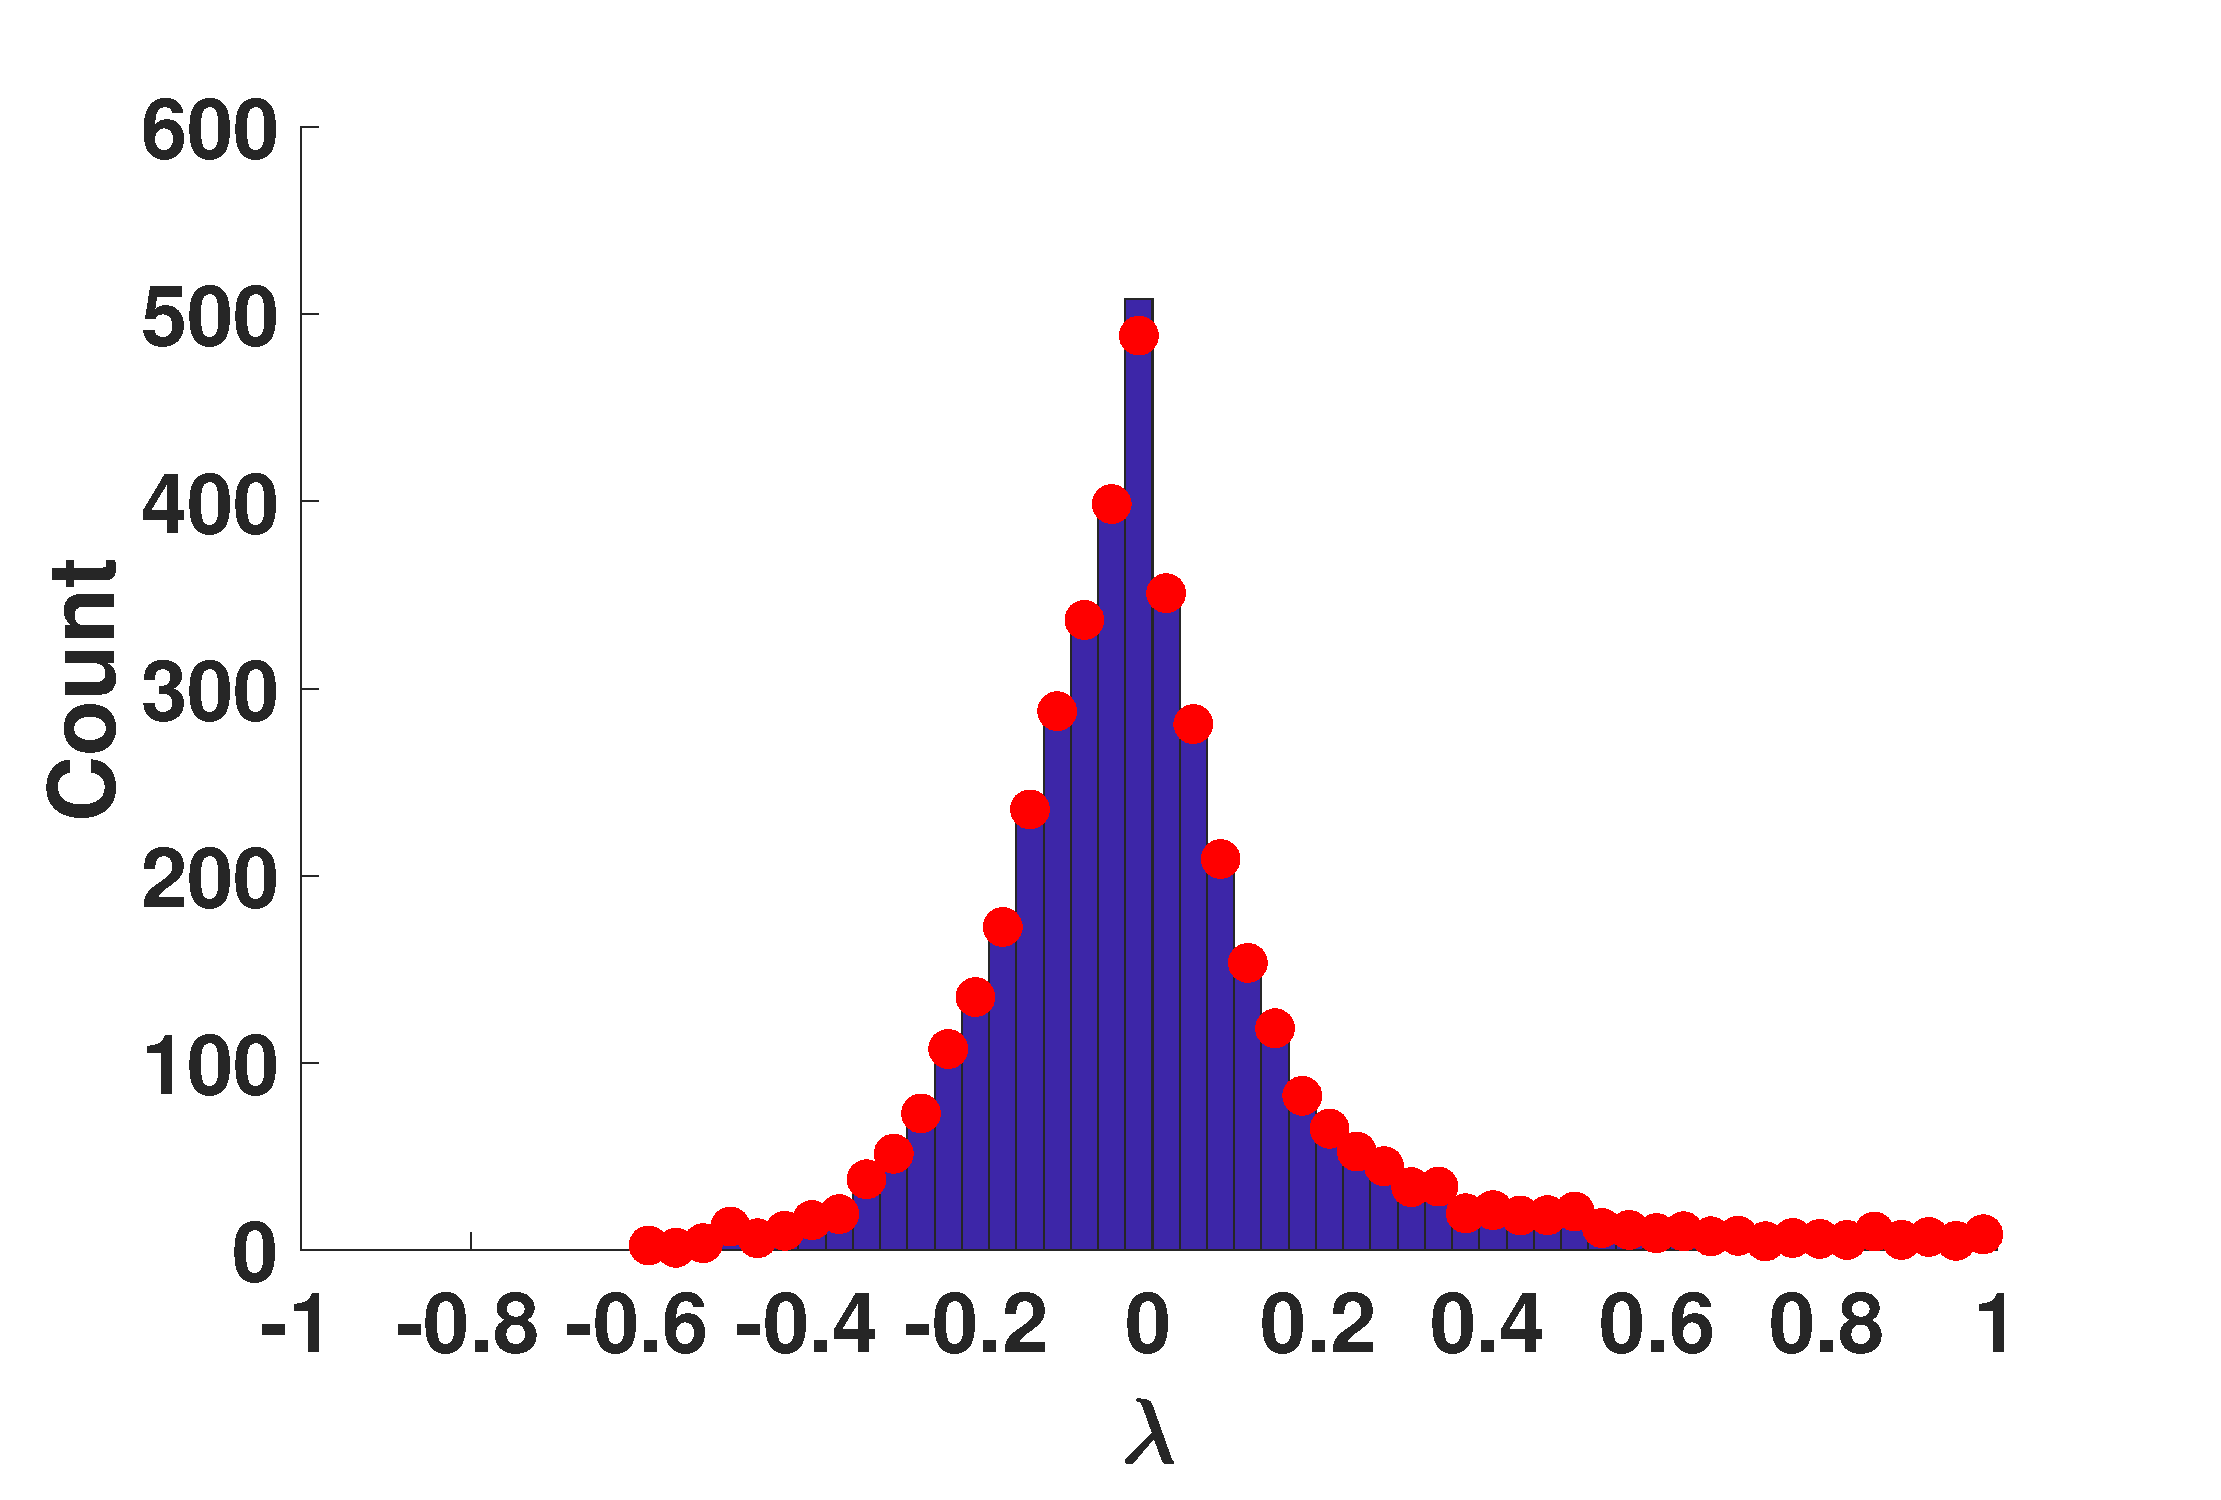
\includegraphics[width=\textwidth,trim = .4cm 0.5cm 3.5cm 1.3cm,clip]
    {./ndos/pics/facebook}
    \label{fig:facebook_dos}
  \end{subfigure}
  %
  \begin{subfigure}[t]{0.19\textwidth}
    \centering  
    \captionsetup{justification=centering,font=scriptsize}
    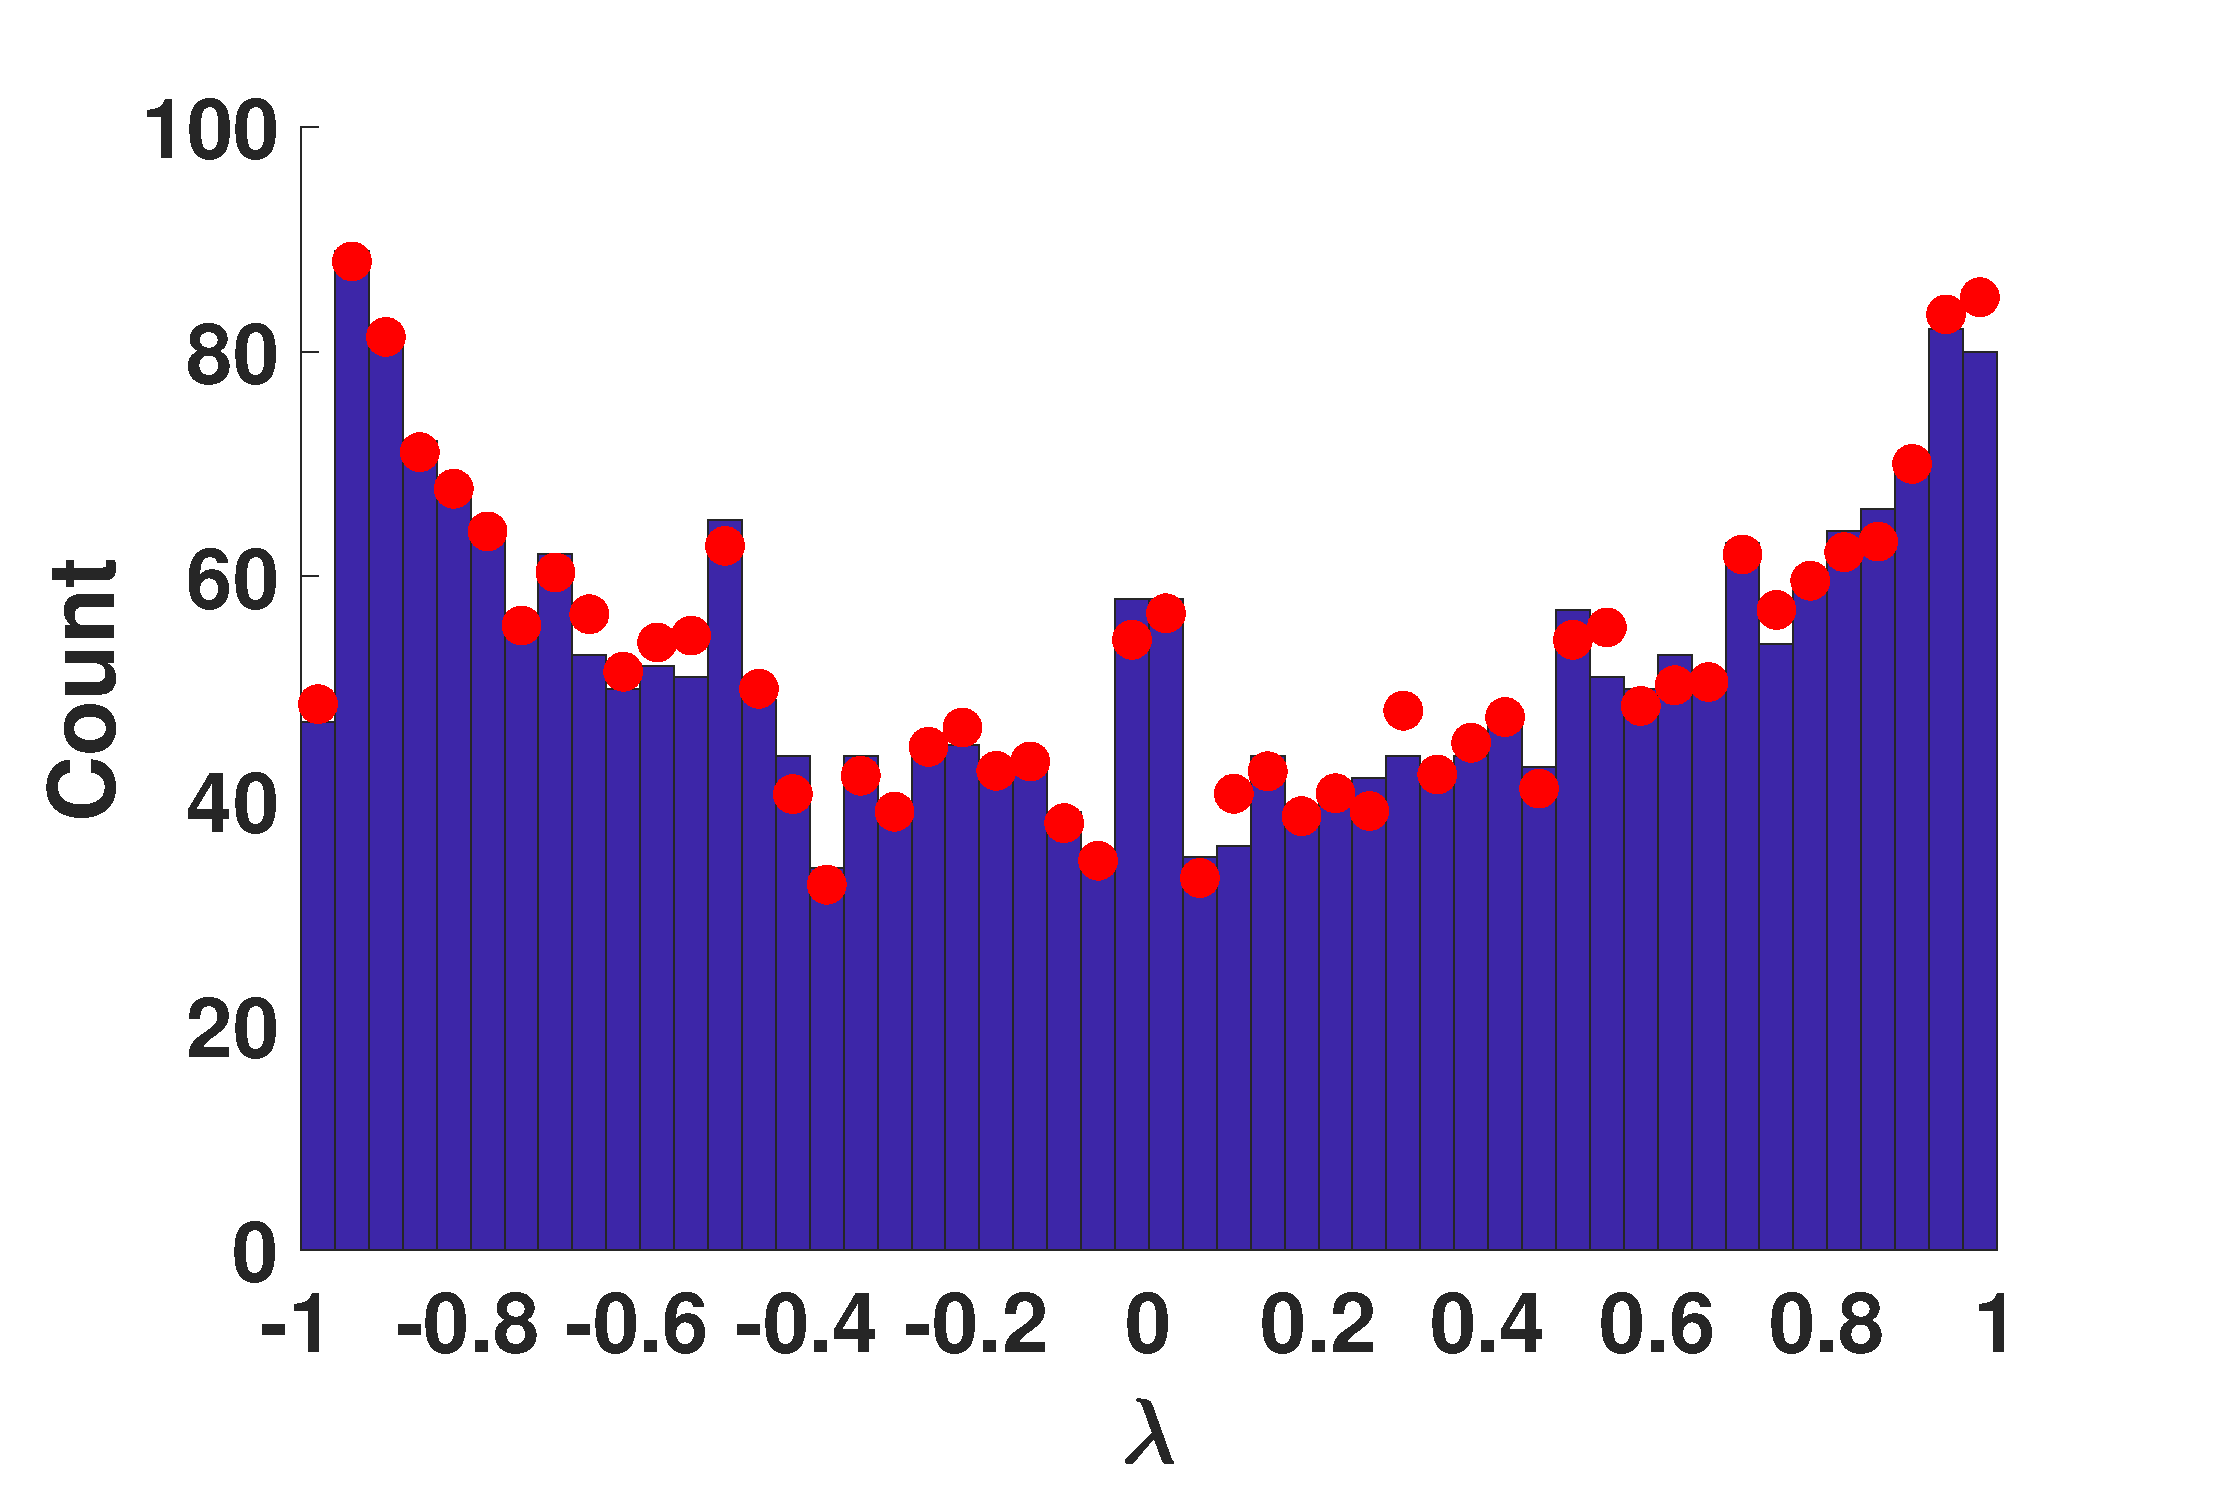
\includegraphics[width=\textwidth,trim = .4cm 0.5cm 3.5cm 1.3cm,clip]
    {./ndos/pics/minnesota}
    \label{fig:minnesota_dos}
  \end{subfigure}
  %
  \begin{subfigure}[t]{0.19\textwidth}
    \centering  
    \captionsetup{justification=centering,font=scriptsize}
    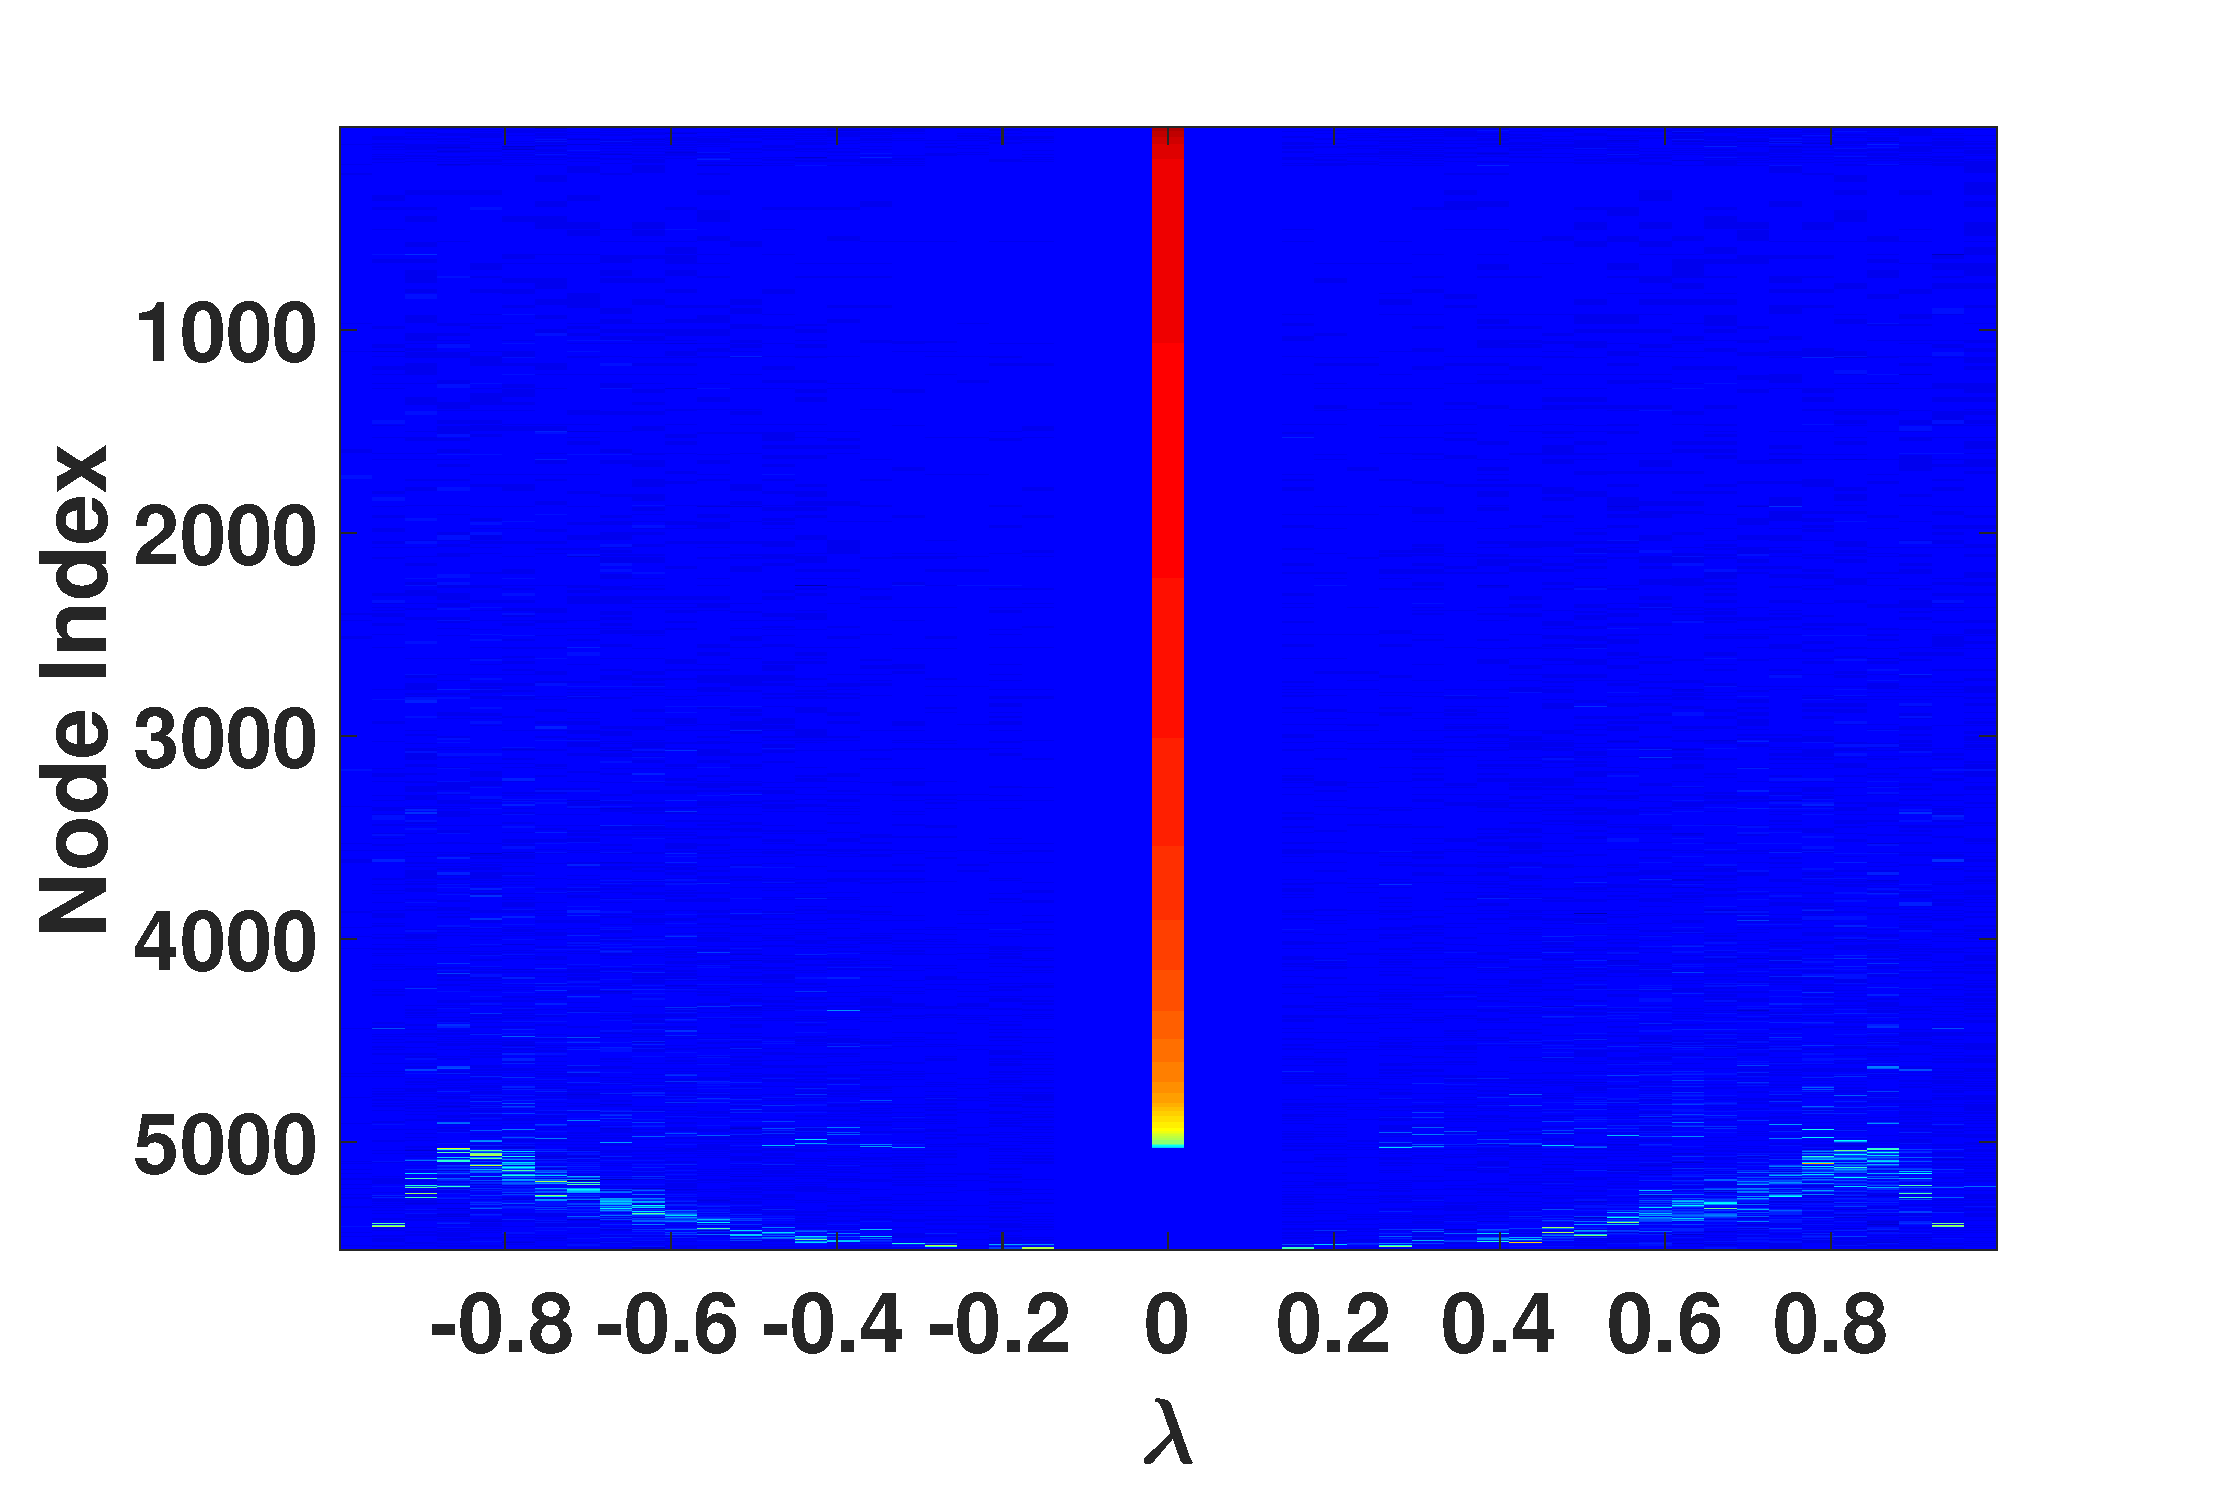
\includegraphics[width=\textwidth,trim = .4cm 0.5cm 3.5cm 1.3cm,clip]
    {./ndos/pics/erdos_ldos}
    \caption{Erd\H{o}s Collaboration Network}
    \label{fig:erdos_ldos}
  \end{subfigure}
  %
  \begin{subfigure}[t]{0.19\textwidth}
    \centering  
    \captionsetup{justification=centering,font=scriptsize}
    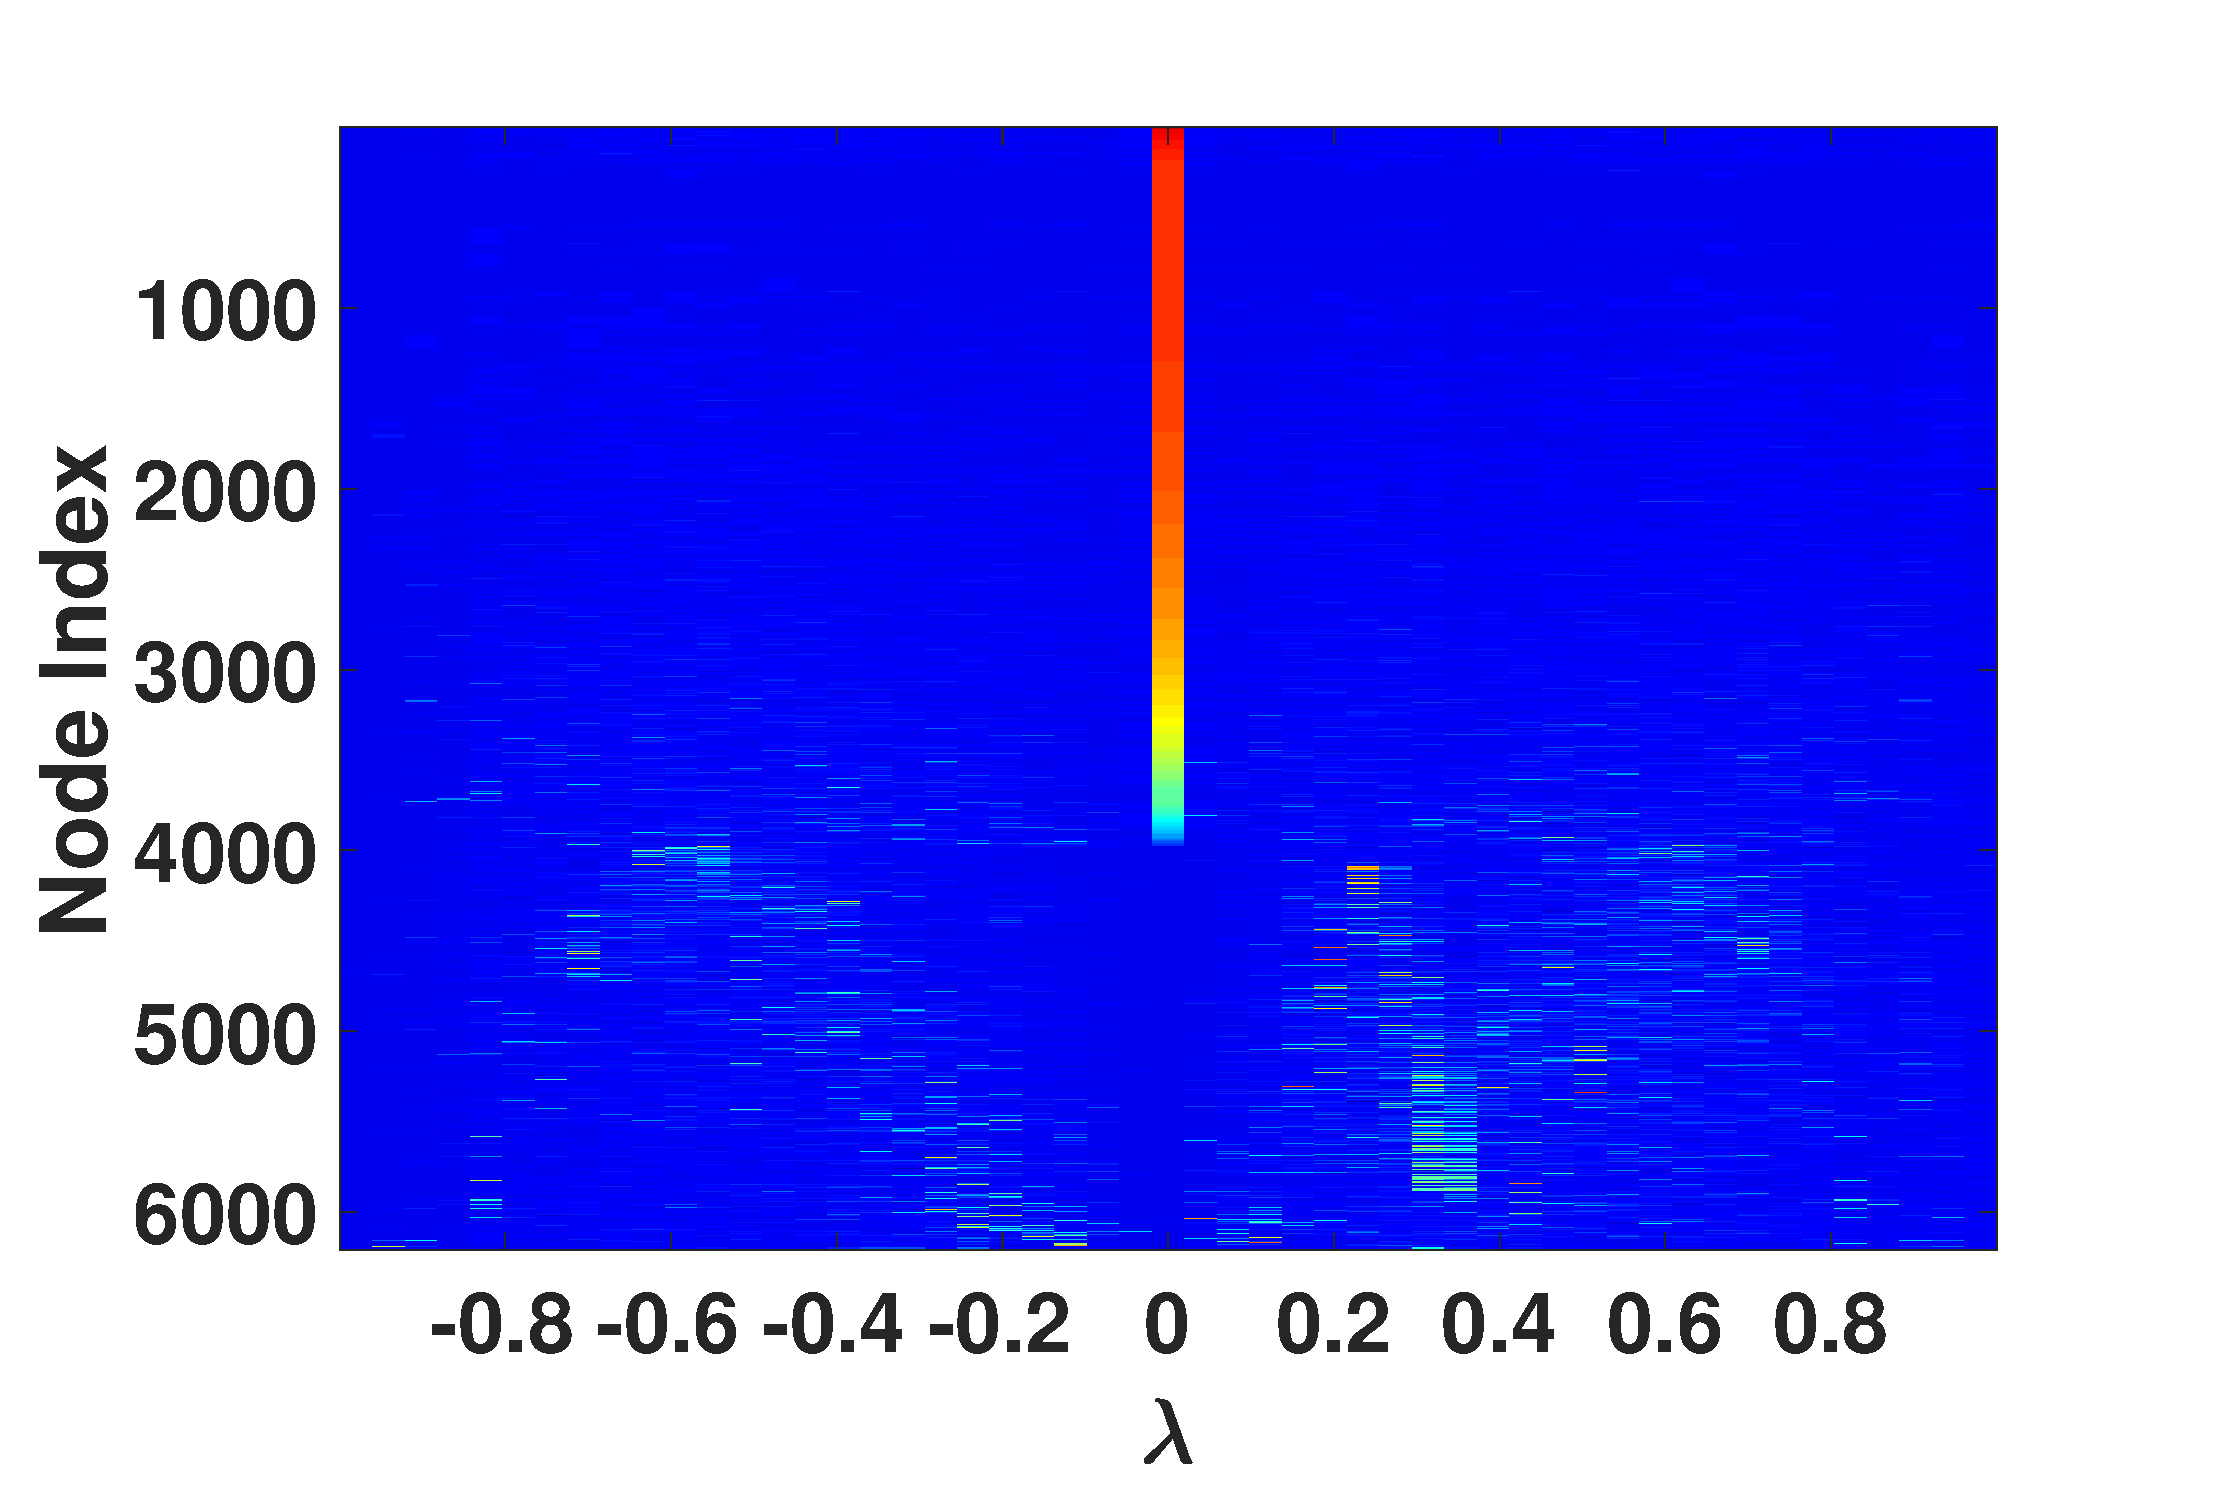
\includegraphics[width=\textwidth,trim = .4cm 0.5cm 3.5cm 1.3cm,clip]
    {./ndos/pics/as19991115_ldos}
    \caption{Autonomous System Network (1999)}
    \label{fig:as_ldos}
  \end{subfigure}
  %
  \begin{subfigure}[t]{0.19\textwidth}
    \centering  
    \captionsetup{justification=centering,font=scriptsize}
    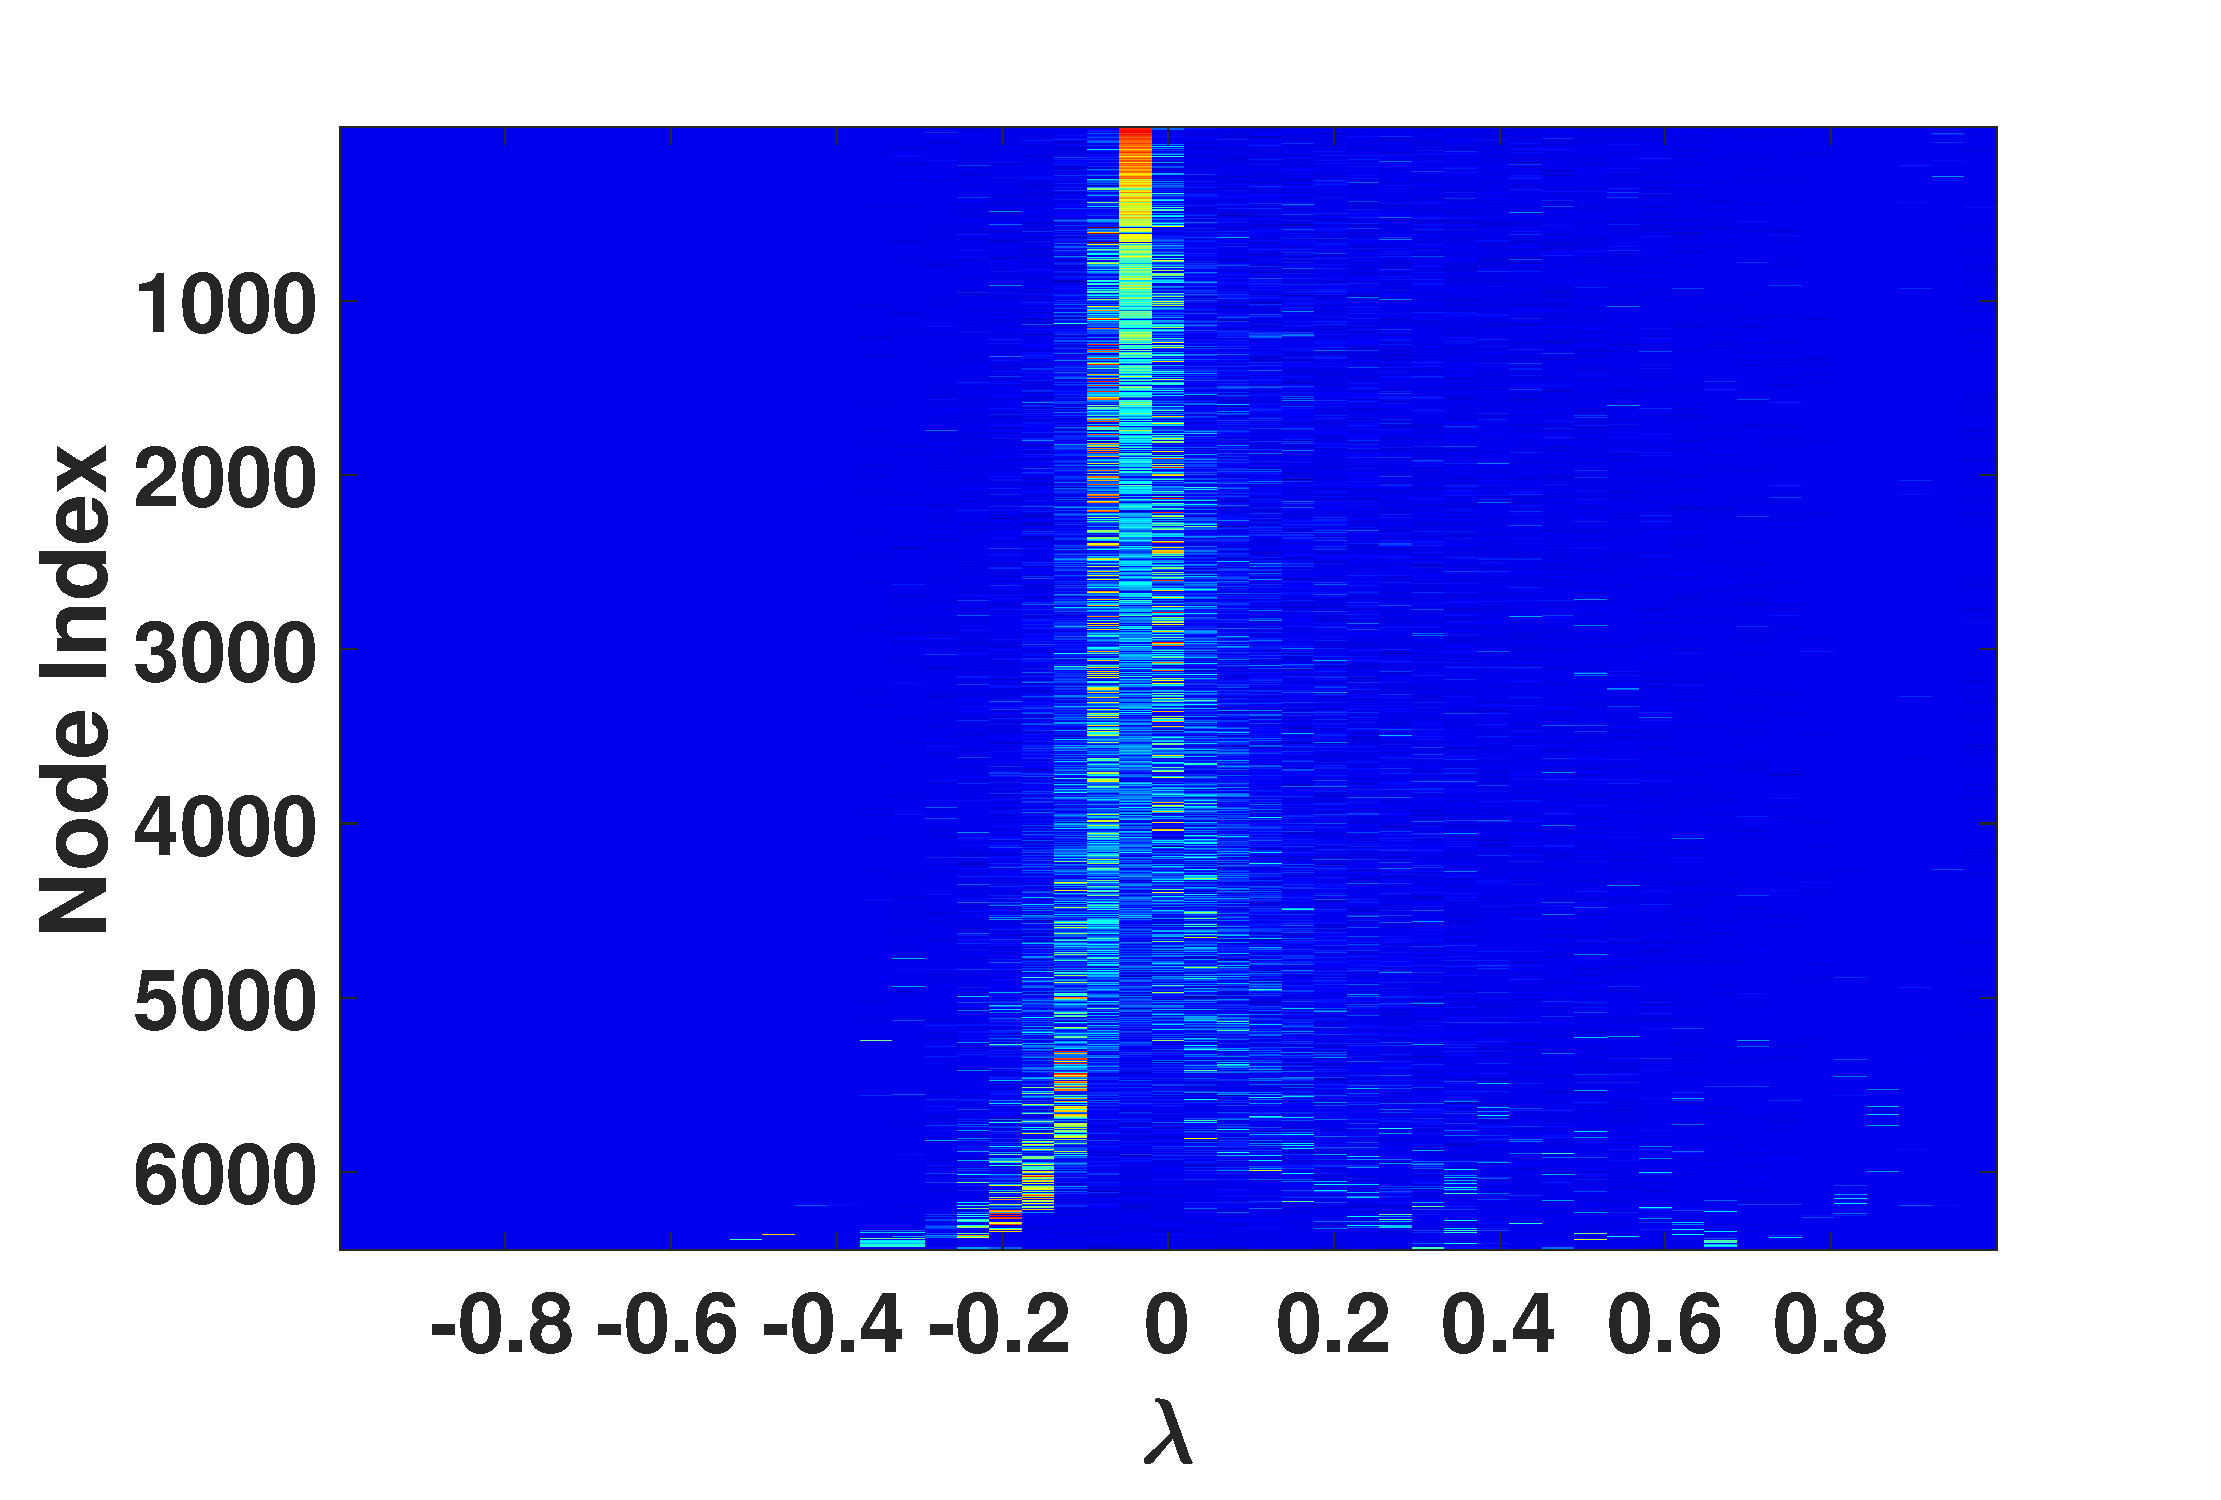
\includegraphics[width=\textwidth,trim = .4cm 0.5cm 3.5cm 1.3cm,clip]
    {./ndos/pics/marvel_ldos}{}
    \caption{Marvel Characters Network}
    \label{fig:marvel_ldos}
  \end{subfigure}
  %
  \begin{subfigure}[t]{0.19\textwidth}
    \centering  
    \captionsetup{justification=centering,font=scriptsize}
    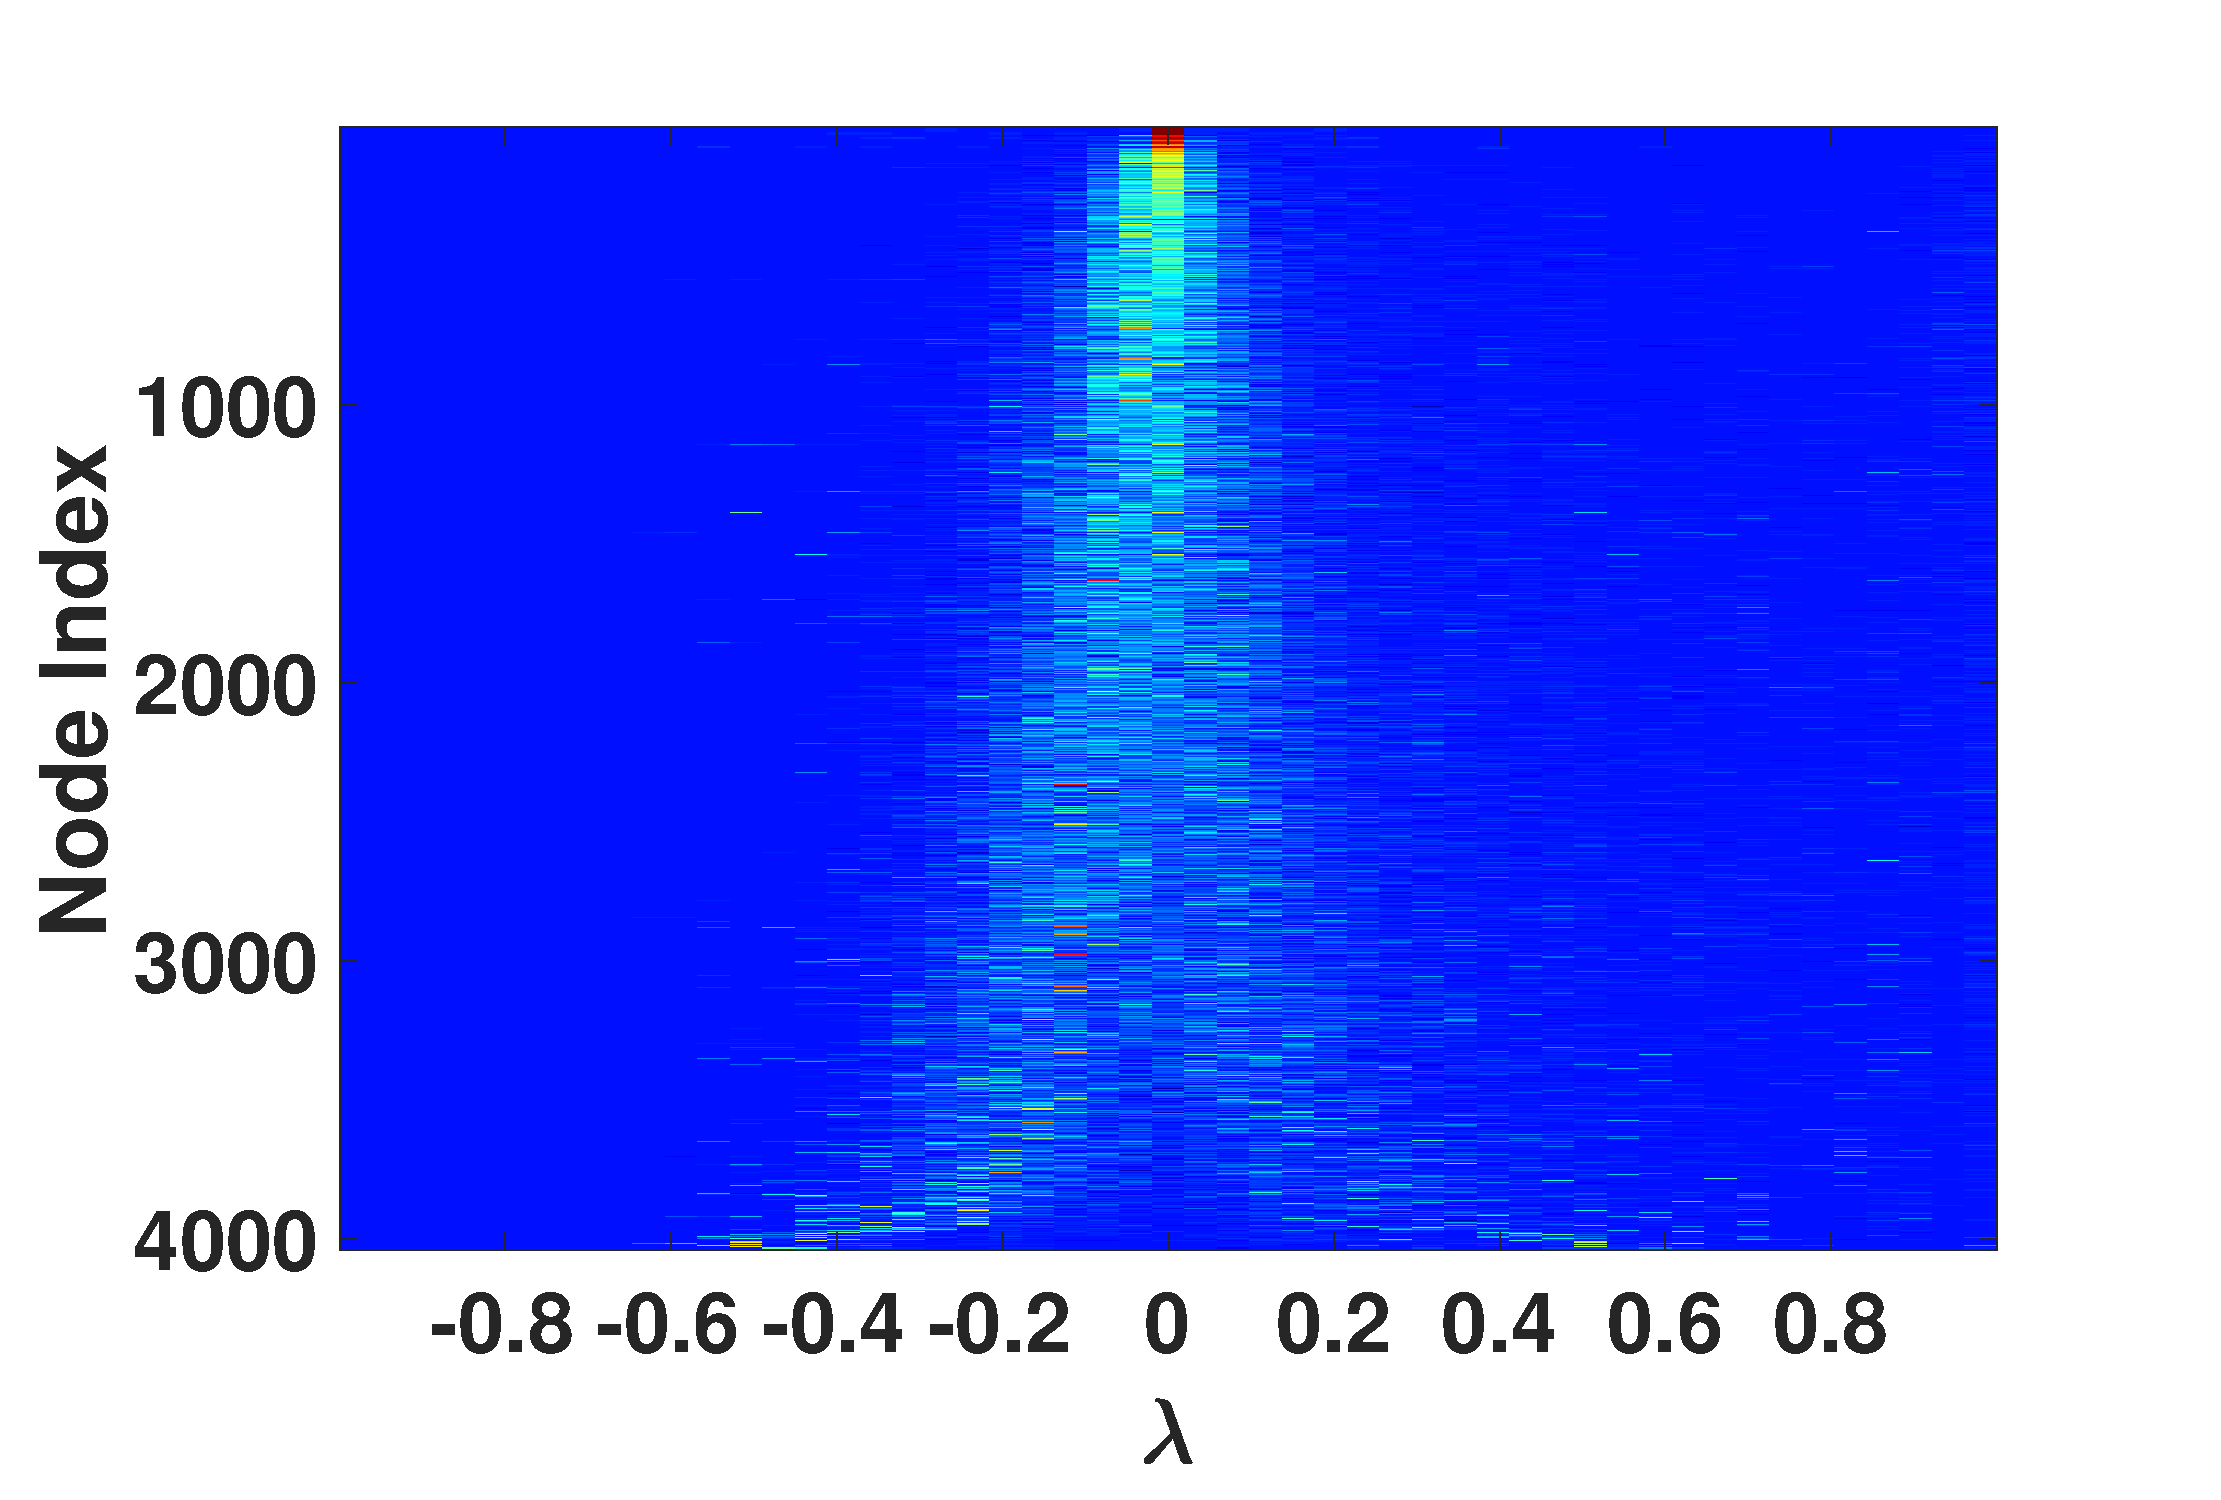
\includegraphics[width=\textwidth,trim = .4cm 0.5cm 3.5cm 1.3cm,clip]
    {./ndos/pics/facebook_ldos}
    \caption{Facebook Ego Networks}
    \label{fig:facebook_ldos}
  \end{subfigure}
  %
  \begin{subfigure}[t]{0.19\textwidth}
    \centering  
    \captionsetup{justification=centering,font=scriptsize}
    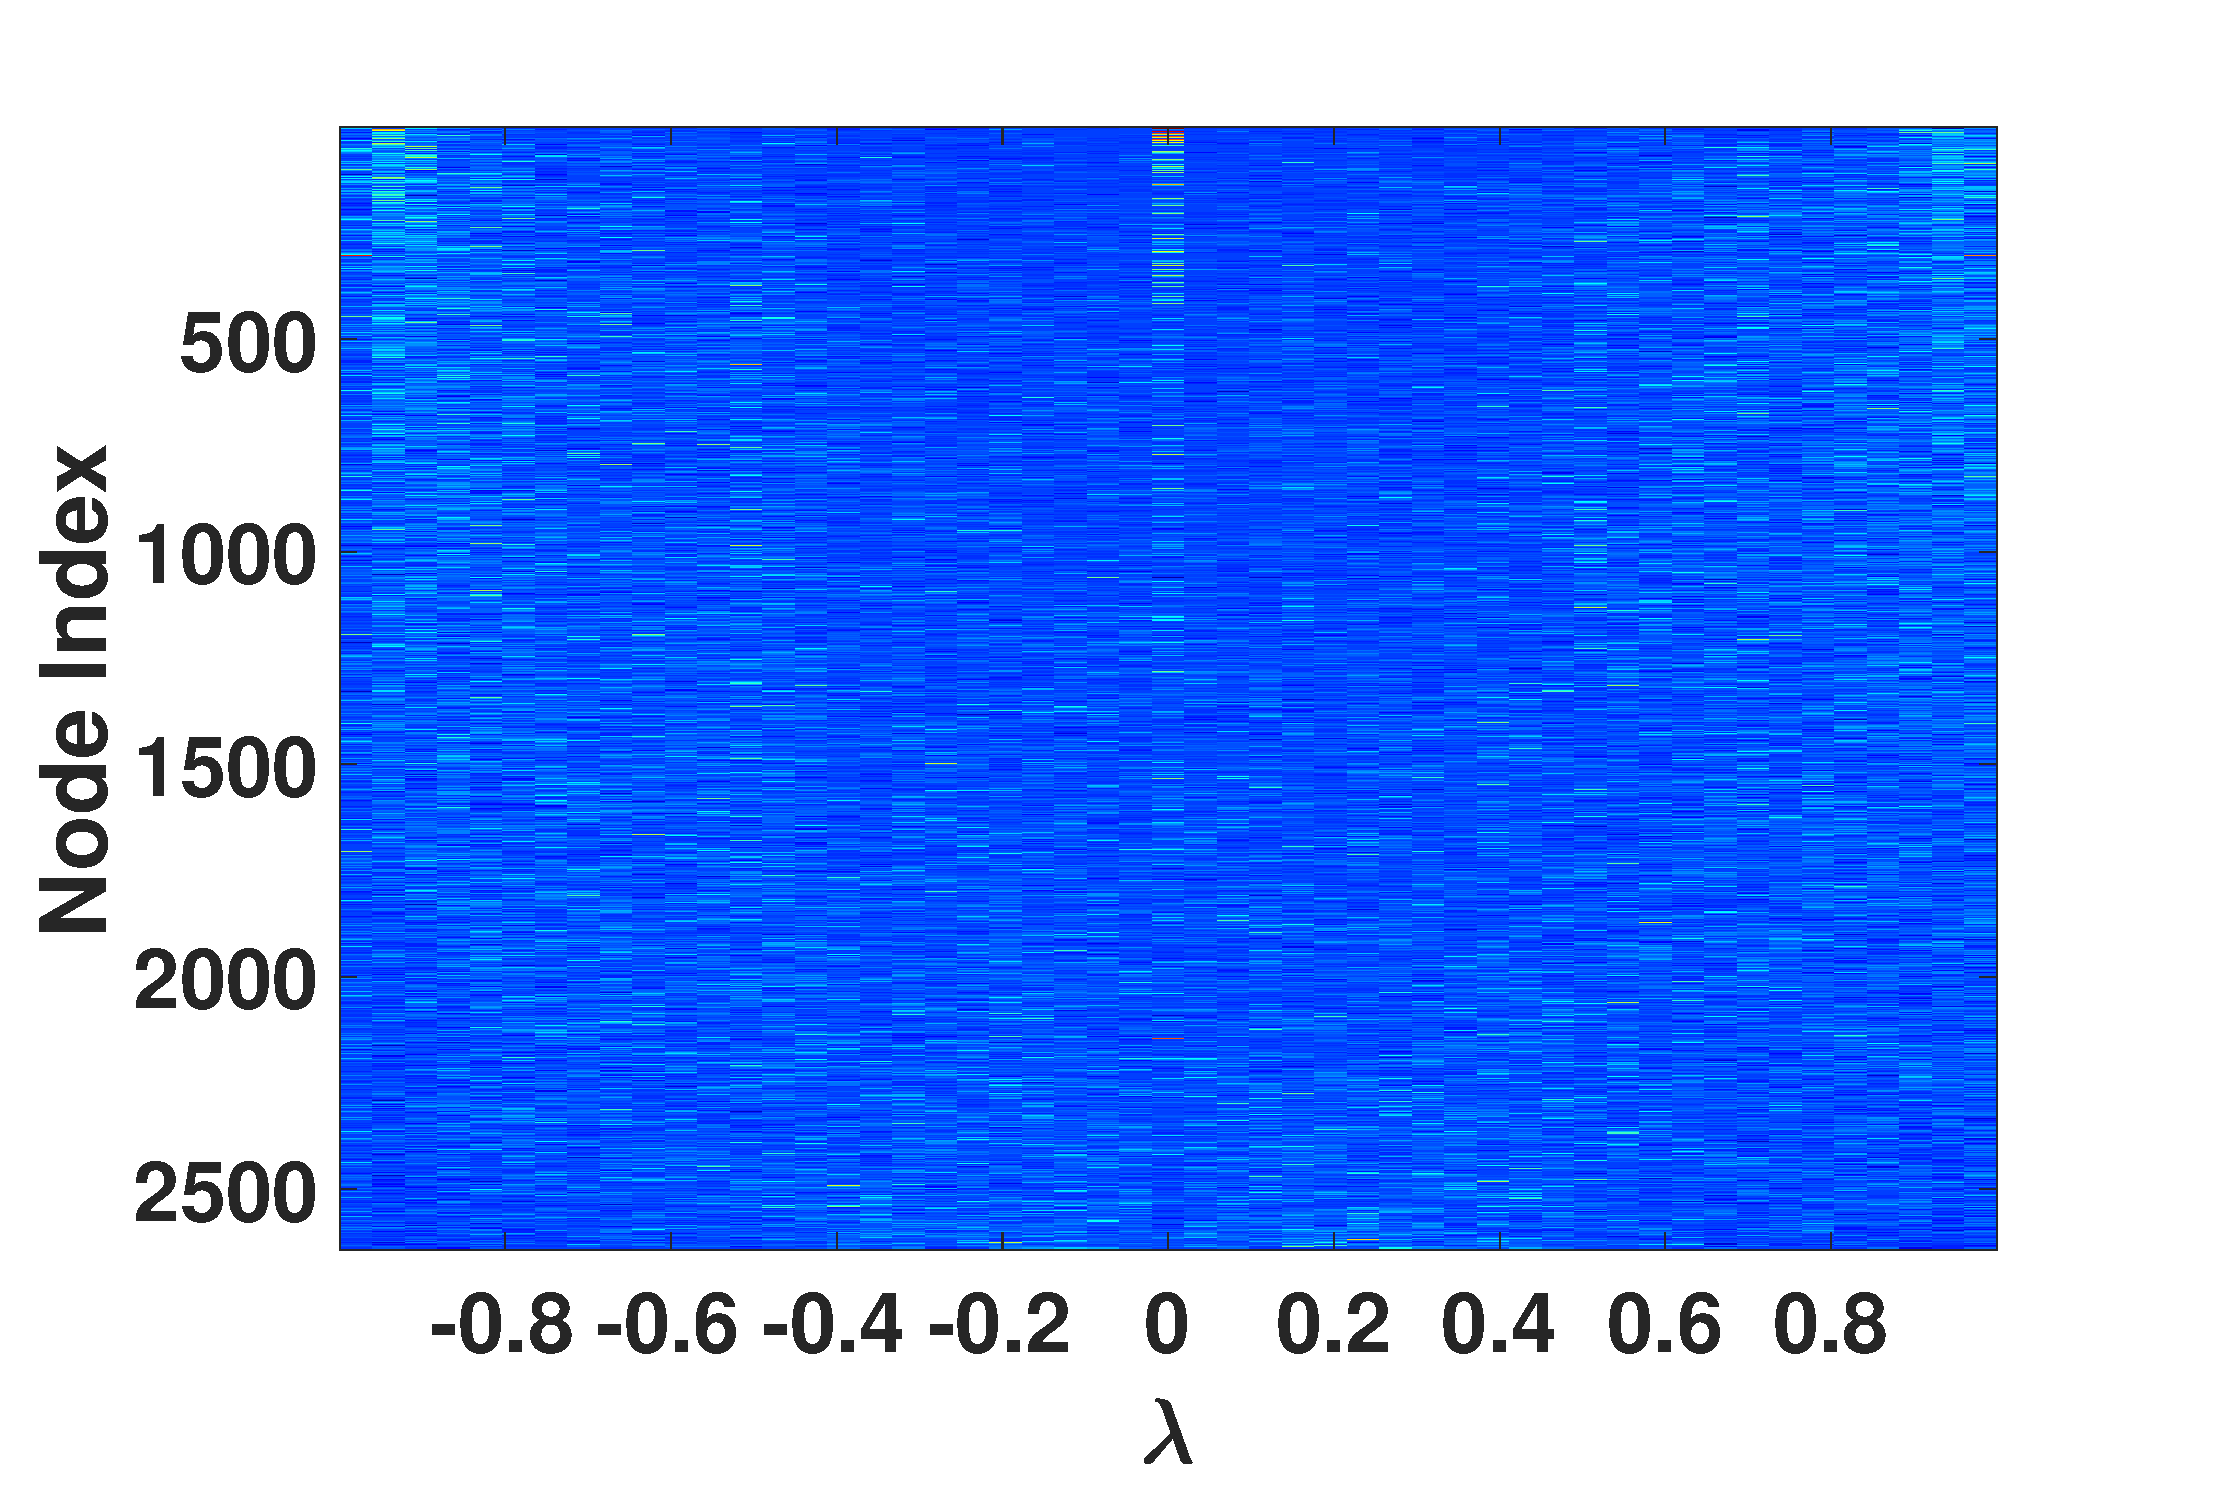
\includegraphics[width=\textwidth,trim = .4cm 0.5cm 3.5cm 1.3cm,clip]
    {./ndos/pics/minnesota_ldos}
    \caption{Minnesota Road Network}
    \label{fig:minnesota_ldos}
  \end{subfigure}
  %
  \begin{subfigure}[t]{0.19\textwidth}
    \centering  
    \captionsetup{justification=centering,font=scriptsize}
    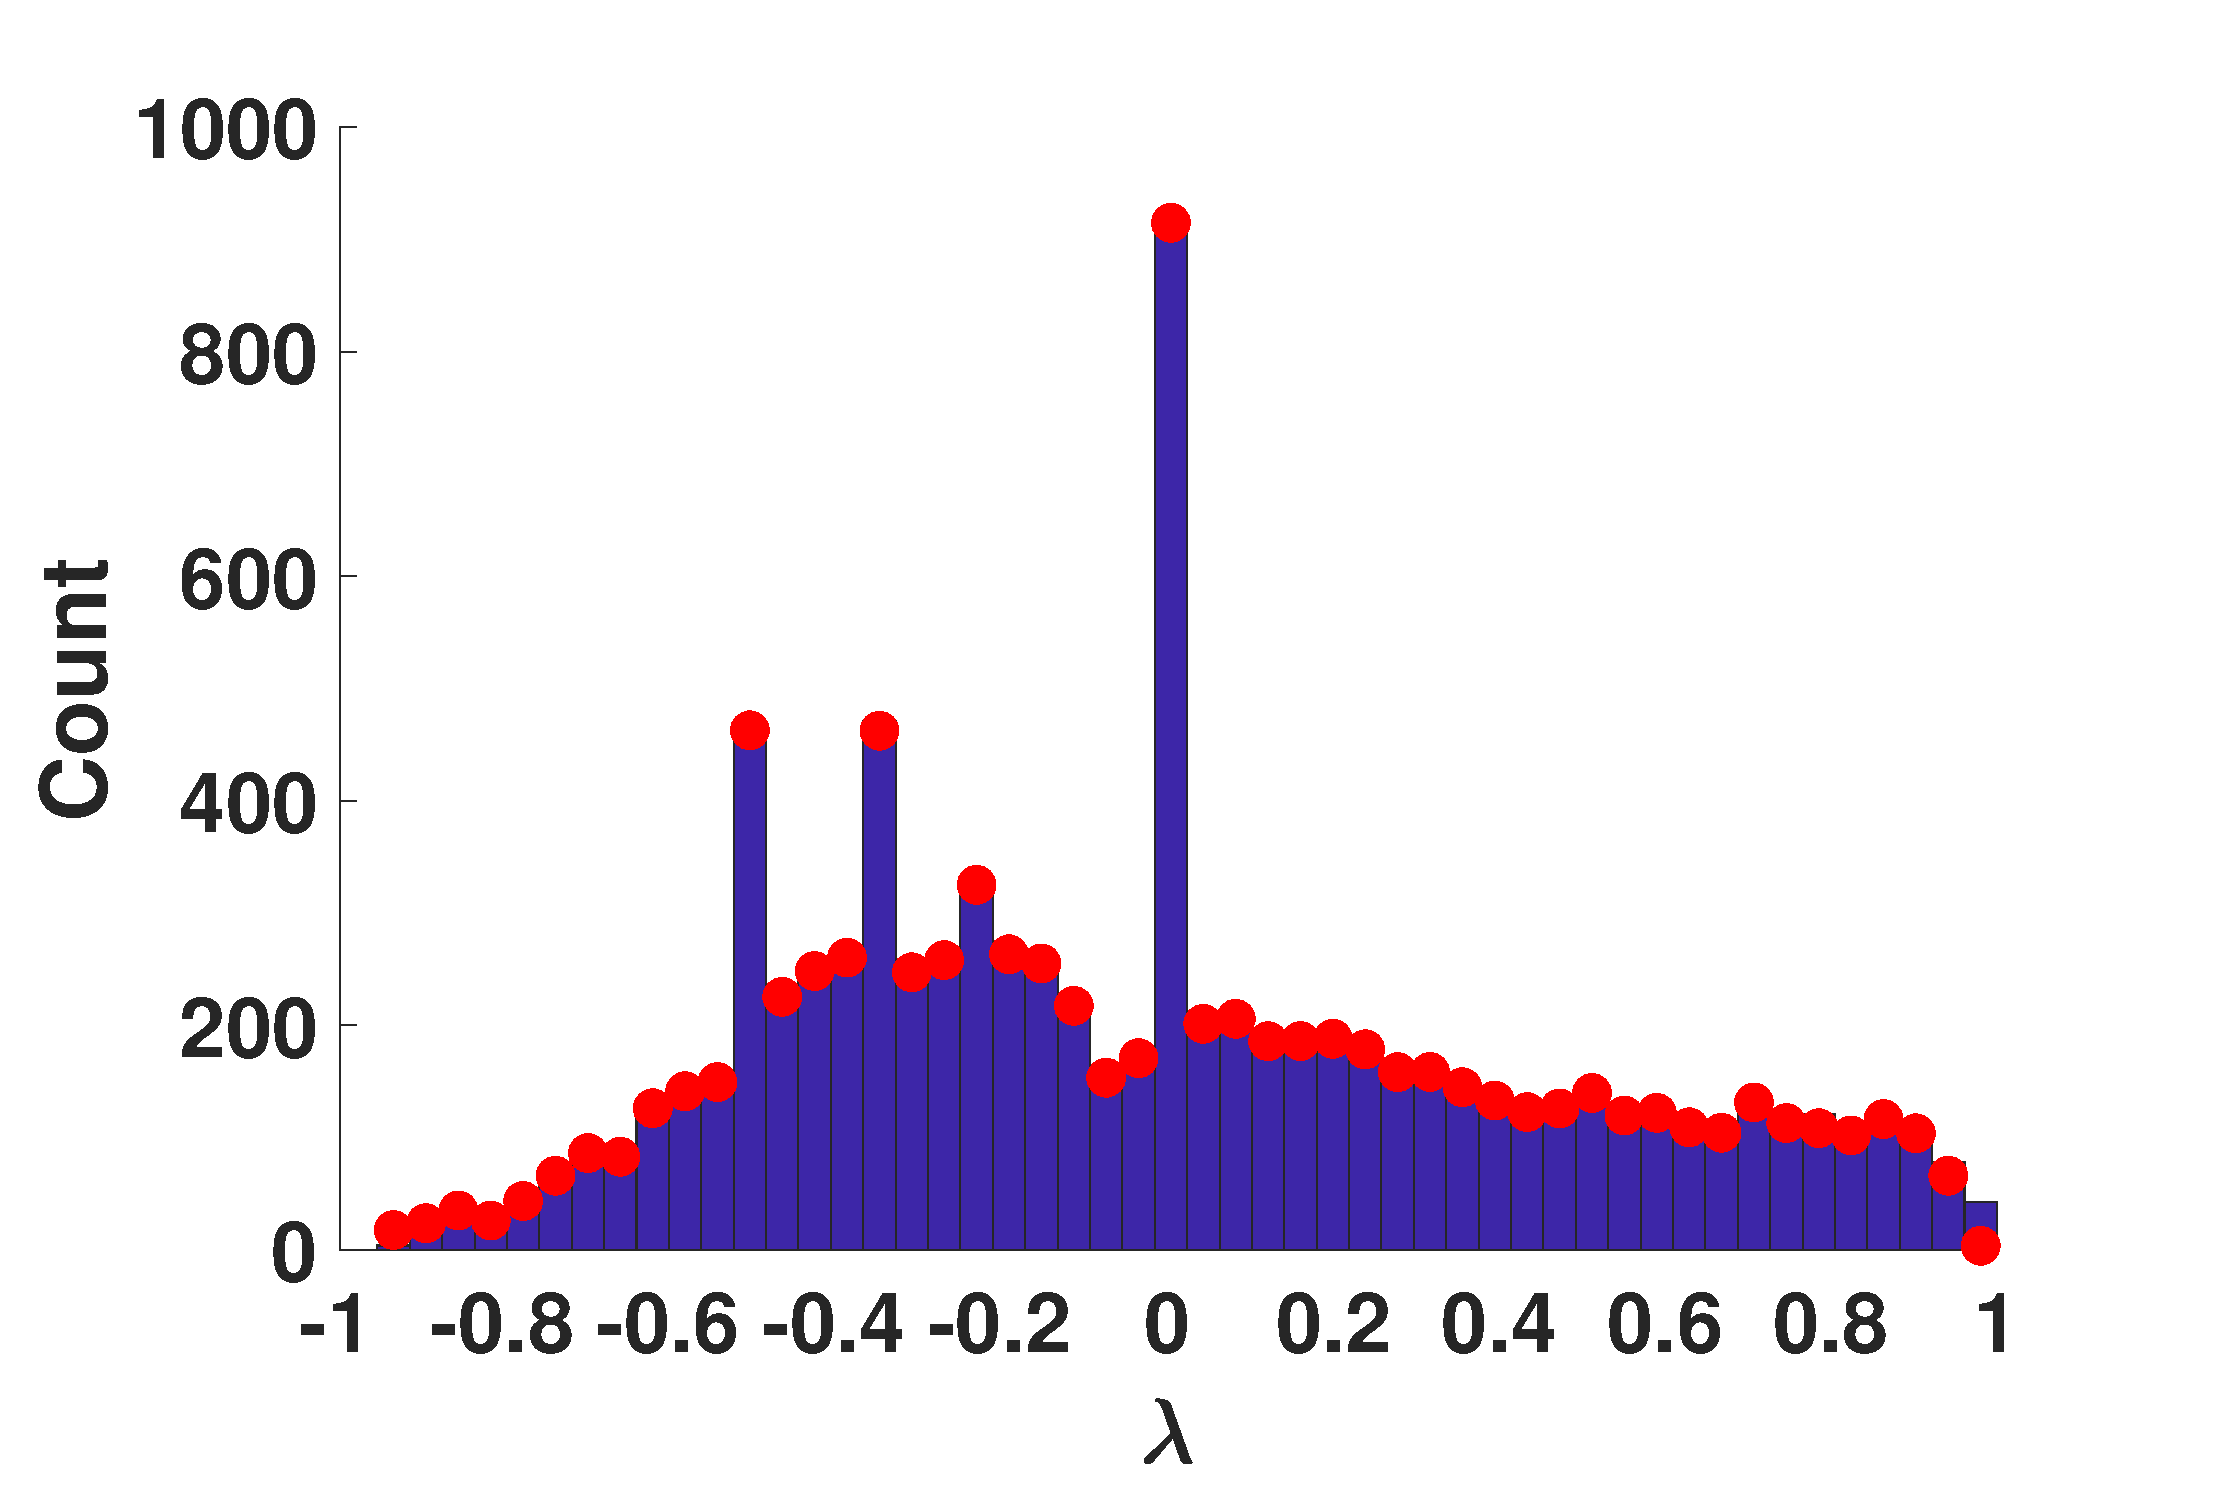
\includegraphics[width=\textwidth,trim = .4cm 0.5cm 3.5cm 1.3cm,clip]
    {./ndos/pics/hepth}
    \label{fig:hepth_dos}
  \end{subfigure}
  %
  \begin{subfigure}[t]{0.19\textwidth}
    \centering  
    \captionsetup{justification=centering,font=scriptsize}
    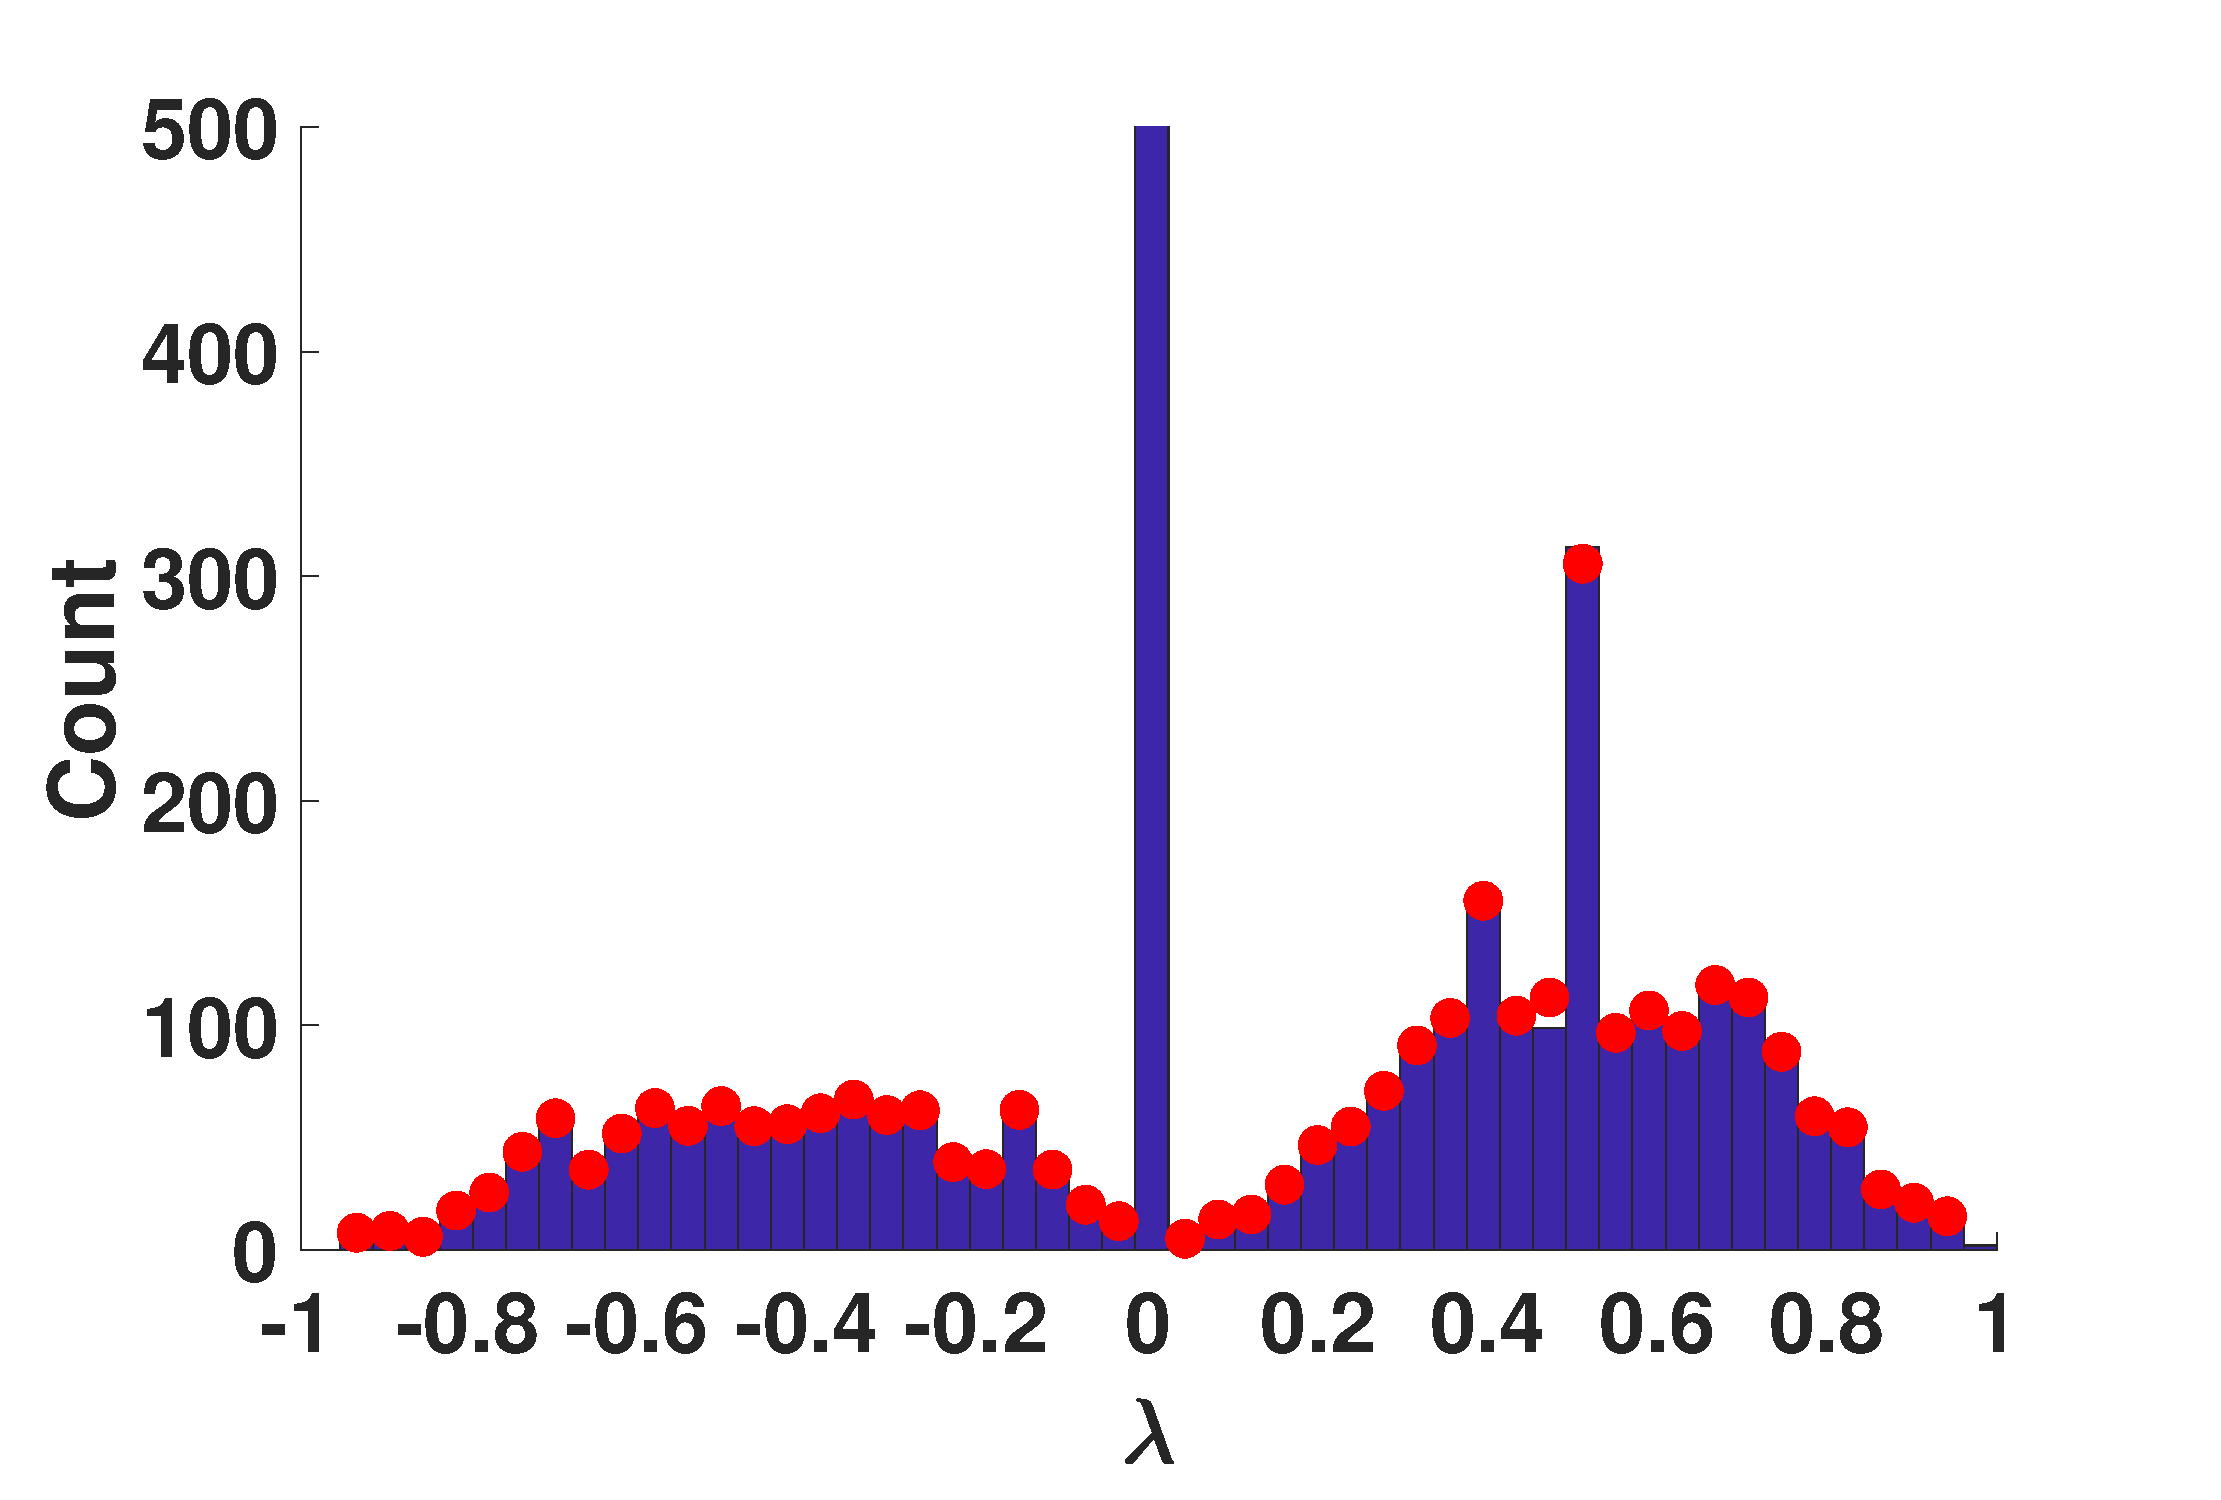
\includegraphics[width=\textwidth,trim = .4cm 0.5cm 3.5cm 1.3cm,clip]
    {./ndos/pics/as20000102}
    \label{fig:as2_dos}
  \end{subfigure}
  %
  \begin{subfigure}[t]{0.19\textwidth}
    \centering
    \captionsetup{justification=centering,font=scriptsize}
    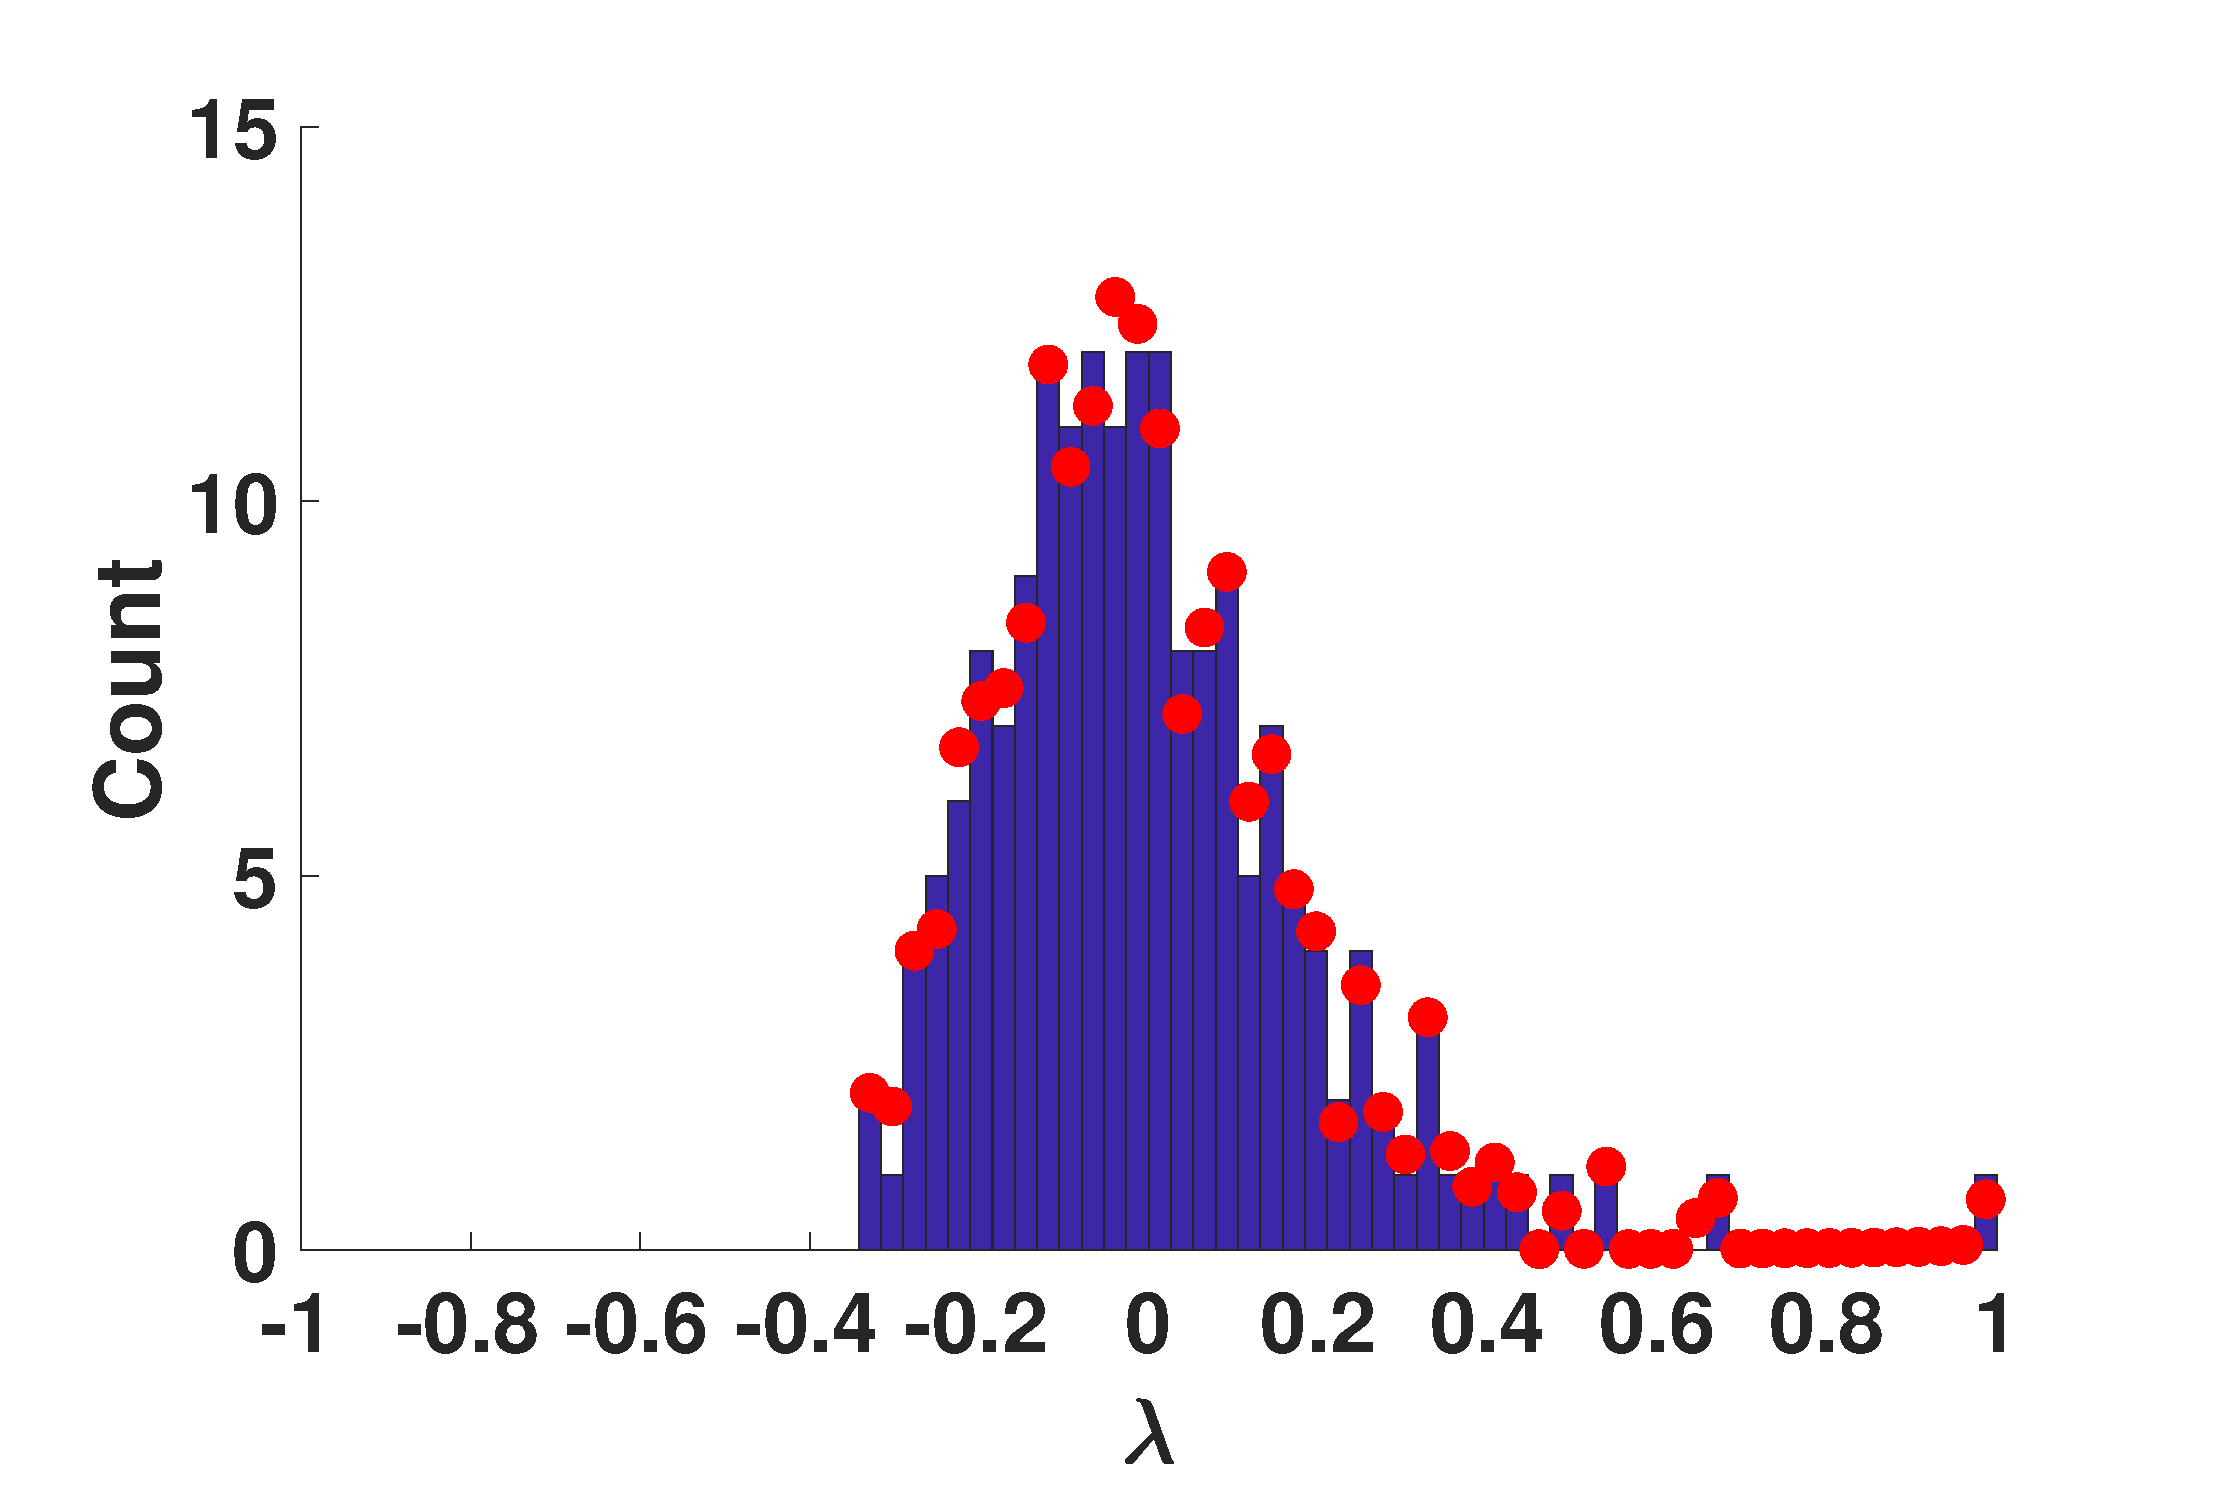
\includegraphics[width=\textwidth,trim = .4cm 0.5cm 3.5cm 1.3cm,clip]
    {./ndos/pics/hp}
    \label{fig:hp_dos}
  \end{subfigure}
  \begin{subfigure}[t]{0.19\textwidth}
    \centering  
    \captionsetup{justification=centering,font=scriptsize}
    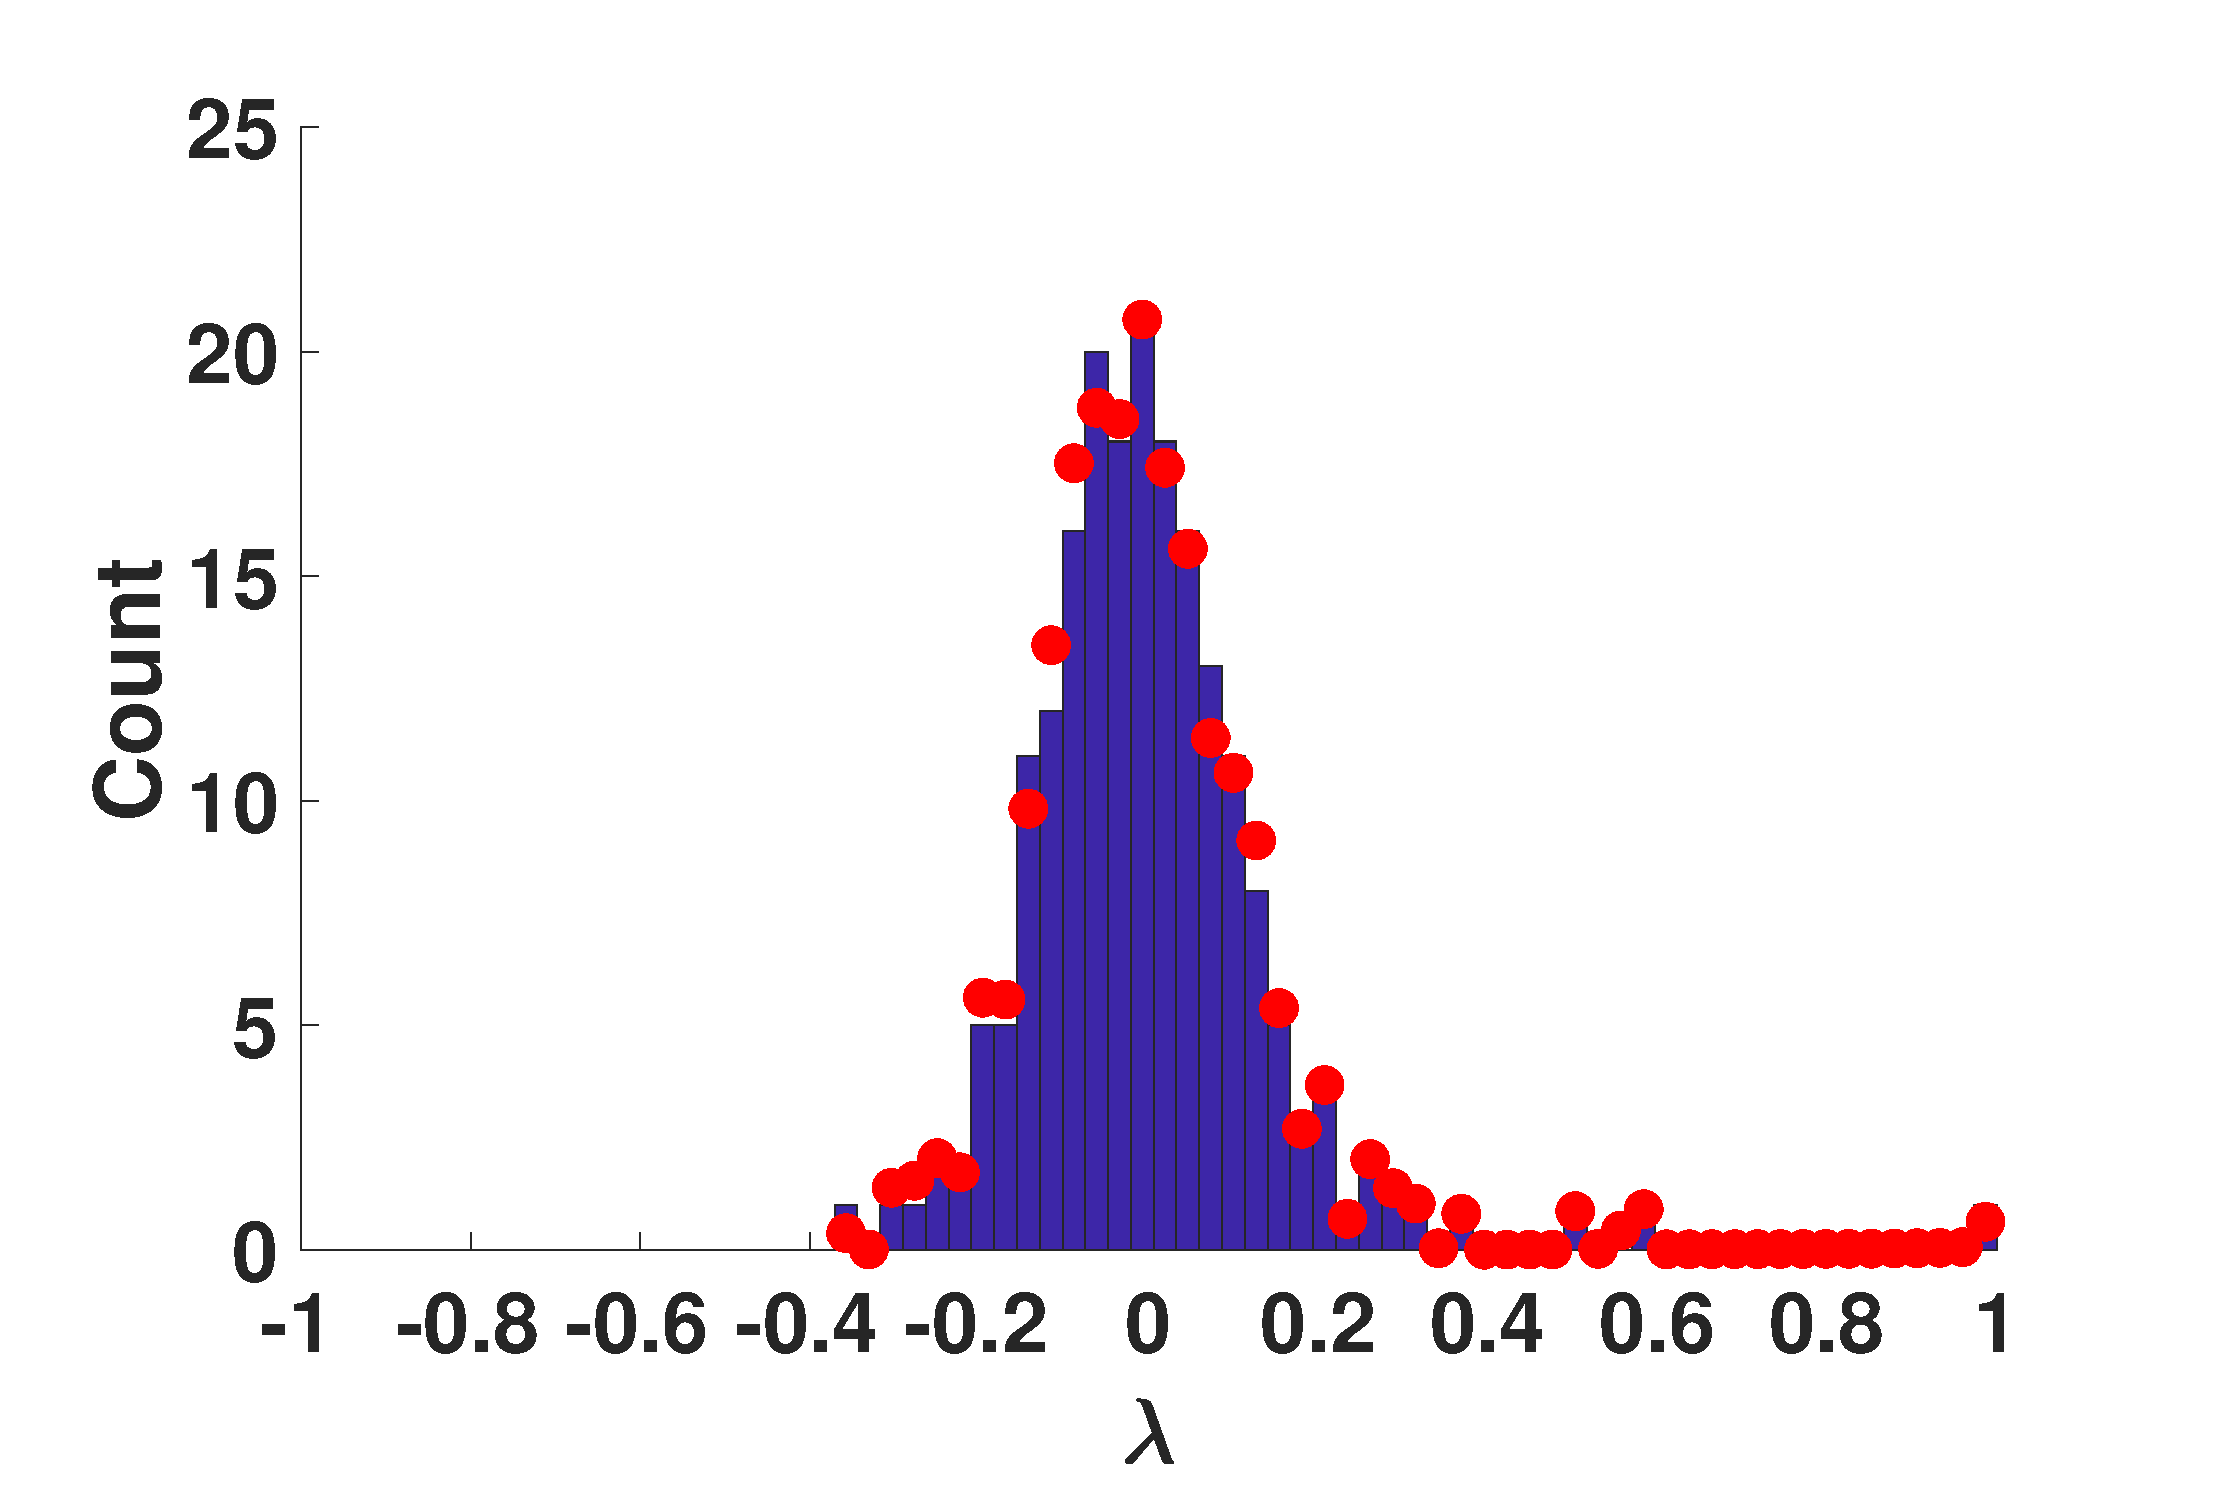
\includegraphics[width=\textwidth,trim = .4cm 0.5cm 3.5cm 1.3cm,clip]
    {./ndos/pics/twitter}
    \label{fig:twitter_dos}
  \end{subfigure}
  %
  \begin{subfigure}[t]{0.19\textwidth}
    \centering  
    \captionsetup{justification=centering,font=scriptsize}
    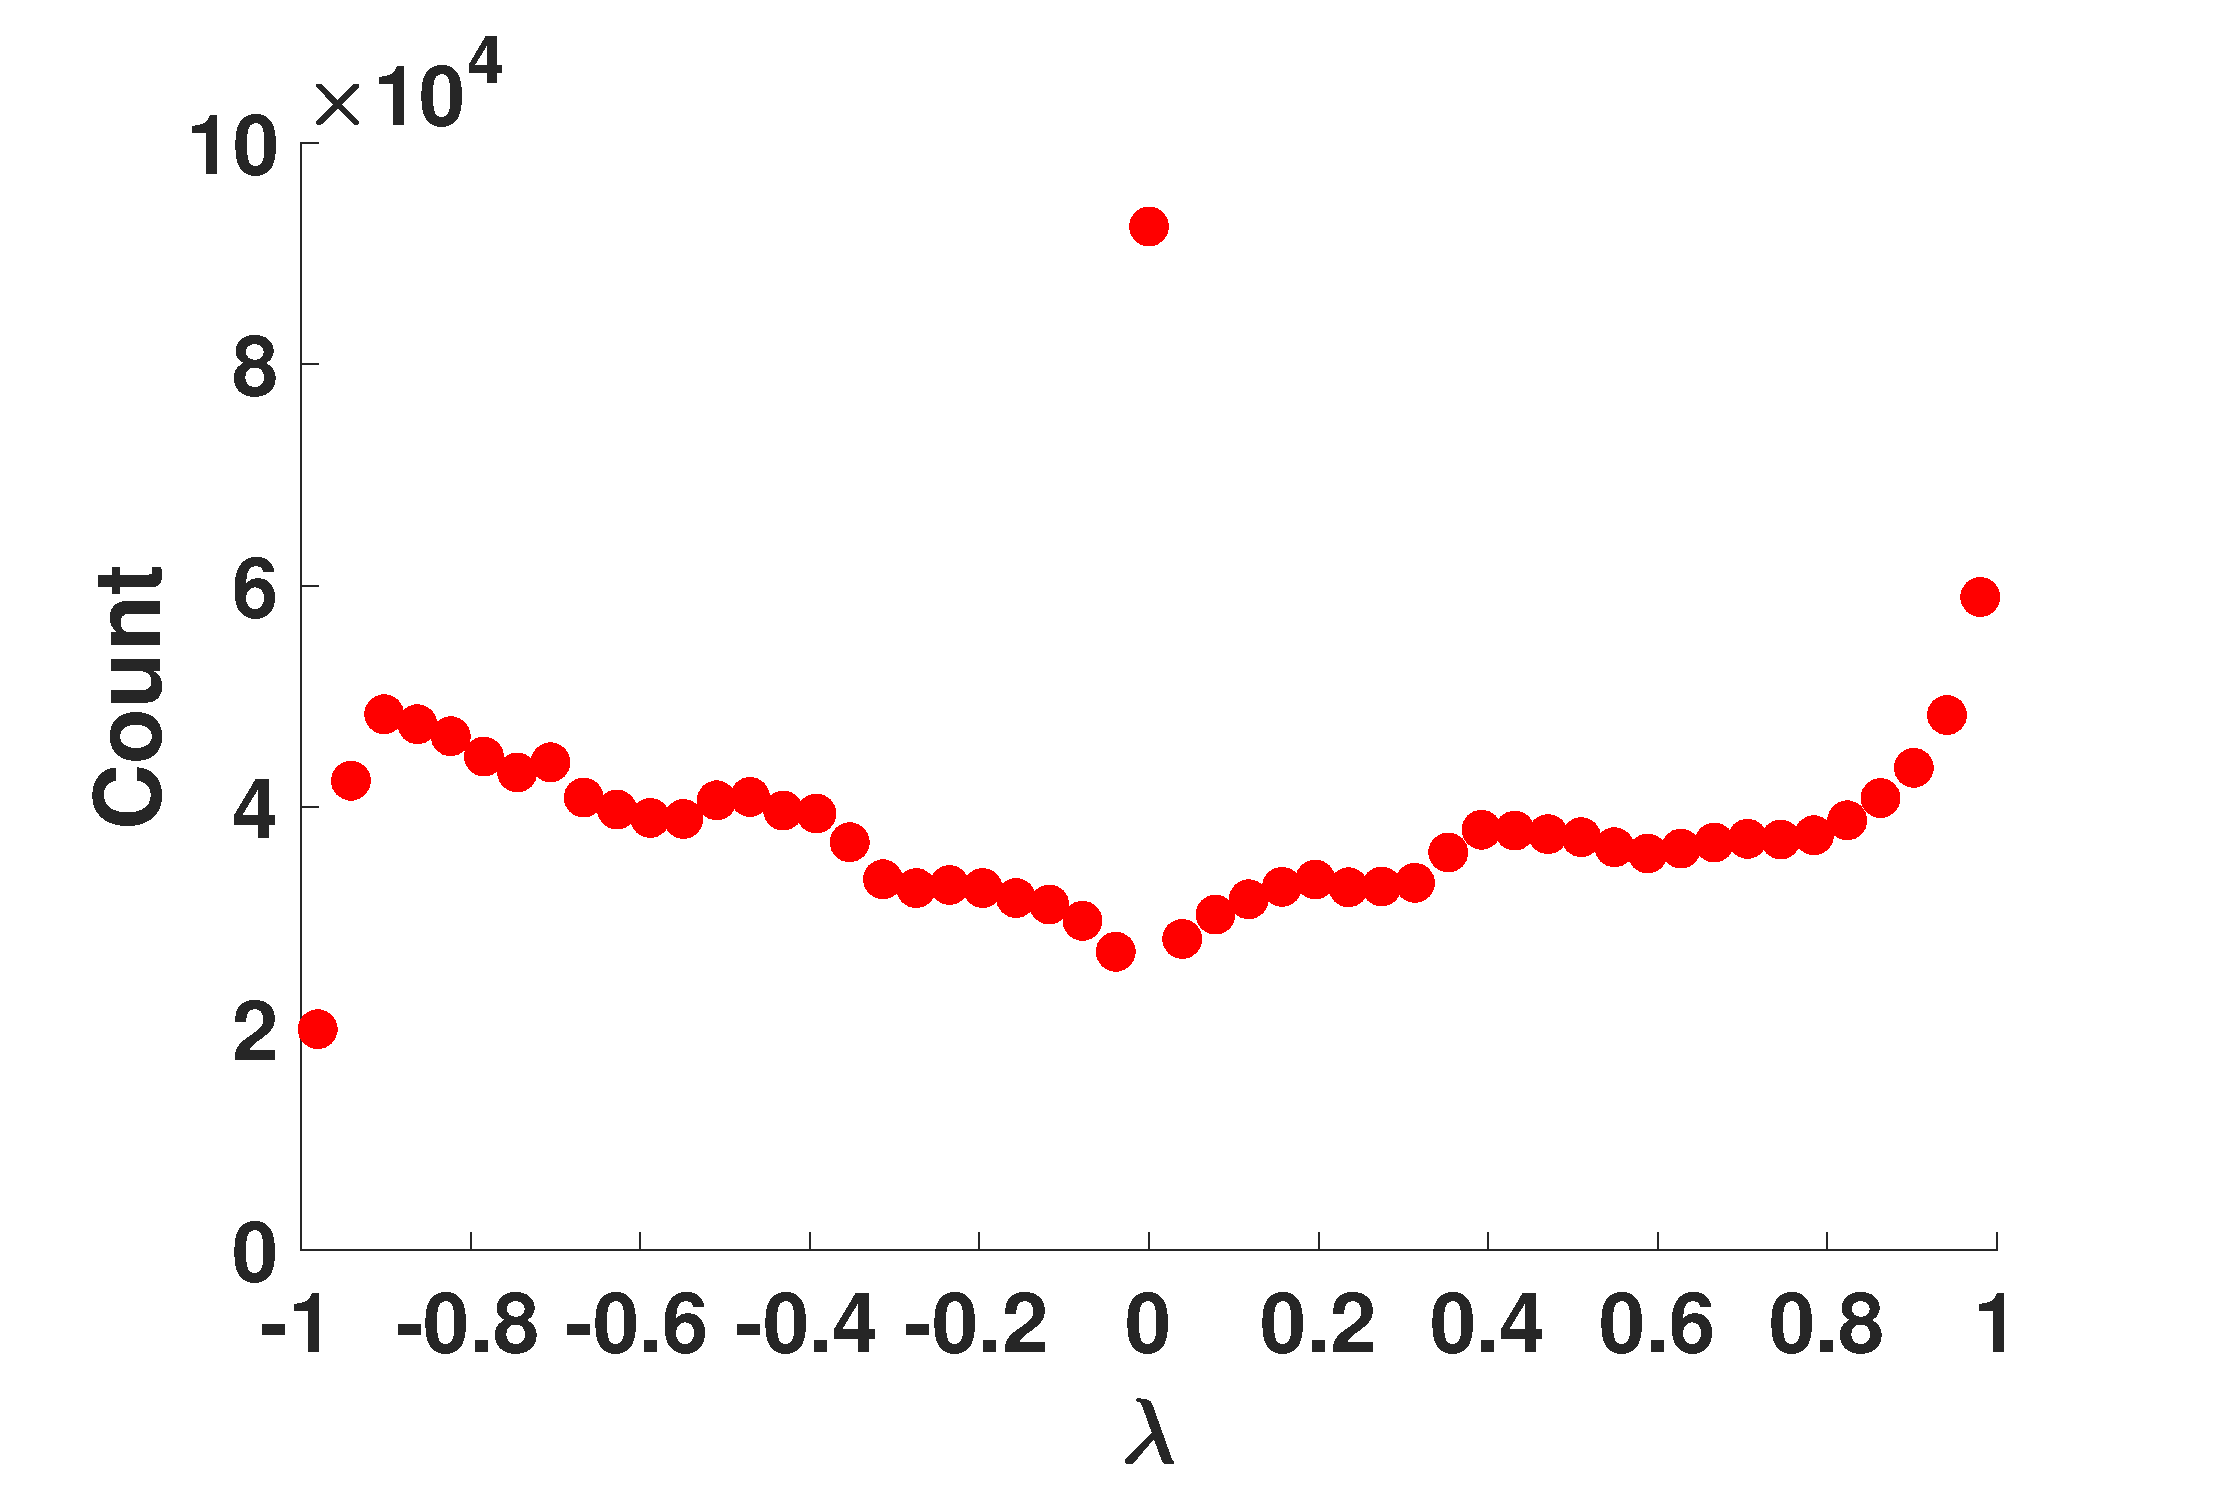
\includegraphics[width=\textwidth,trim = .4cm 0.5cm 3.5cm .3cm,clip]
    {./ndos/pics/roadca}
    \label{fig:roadca_dos}
  \end{subfigure}
  %
  \begin{subfigure}[t]{0.19\textwidth}
    \centering  
    \captionsetup{justification=centering,font=scriptsize}
    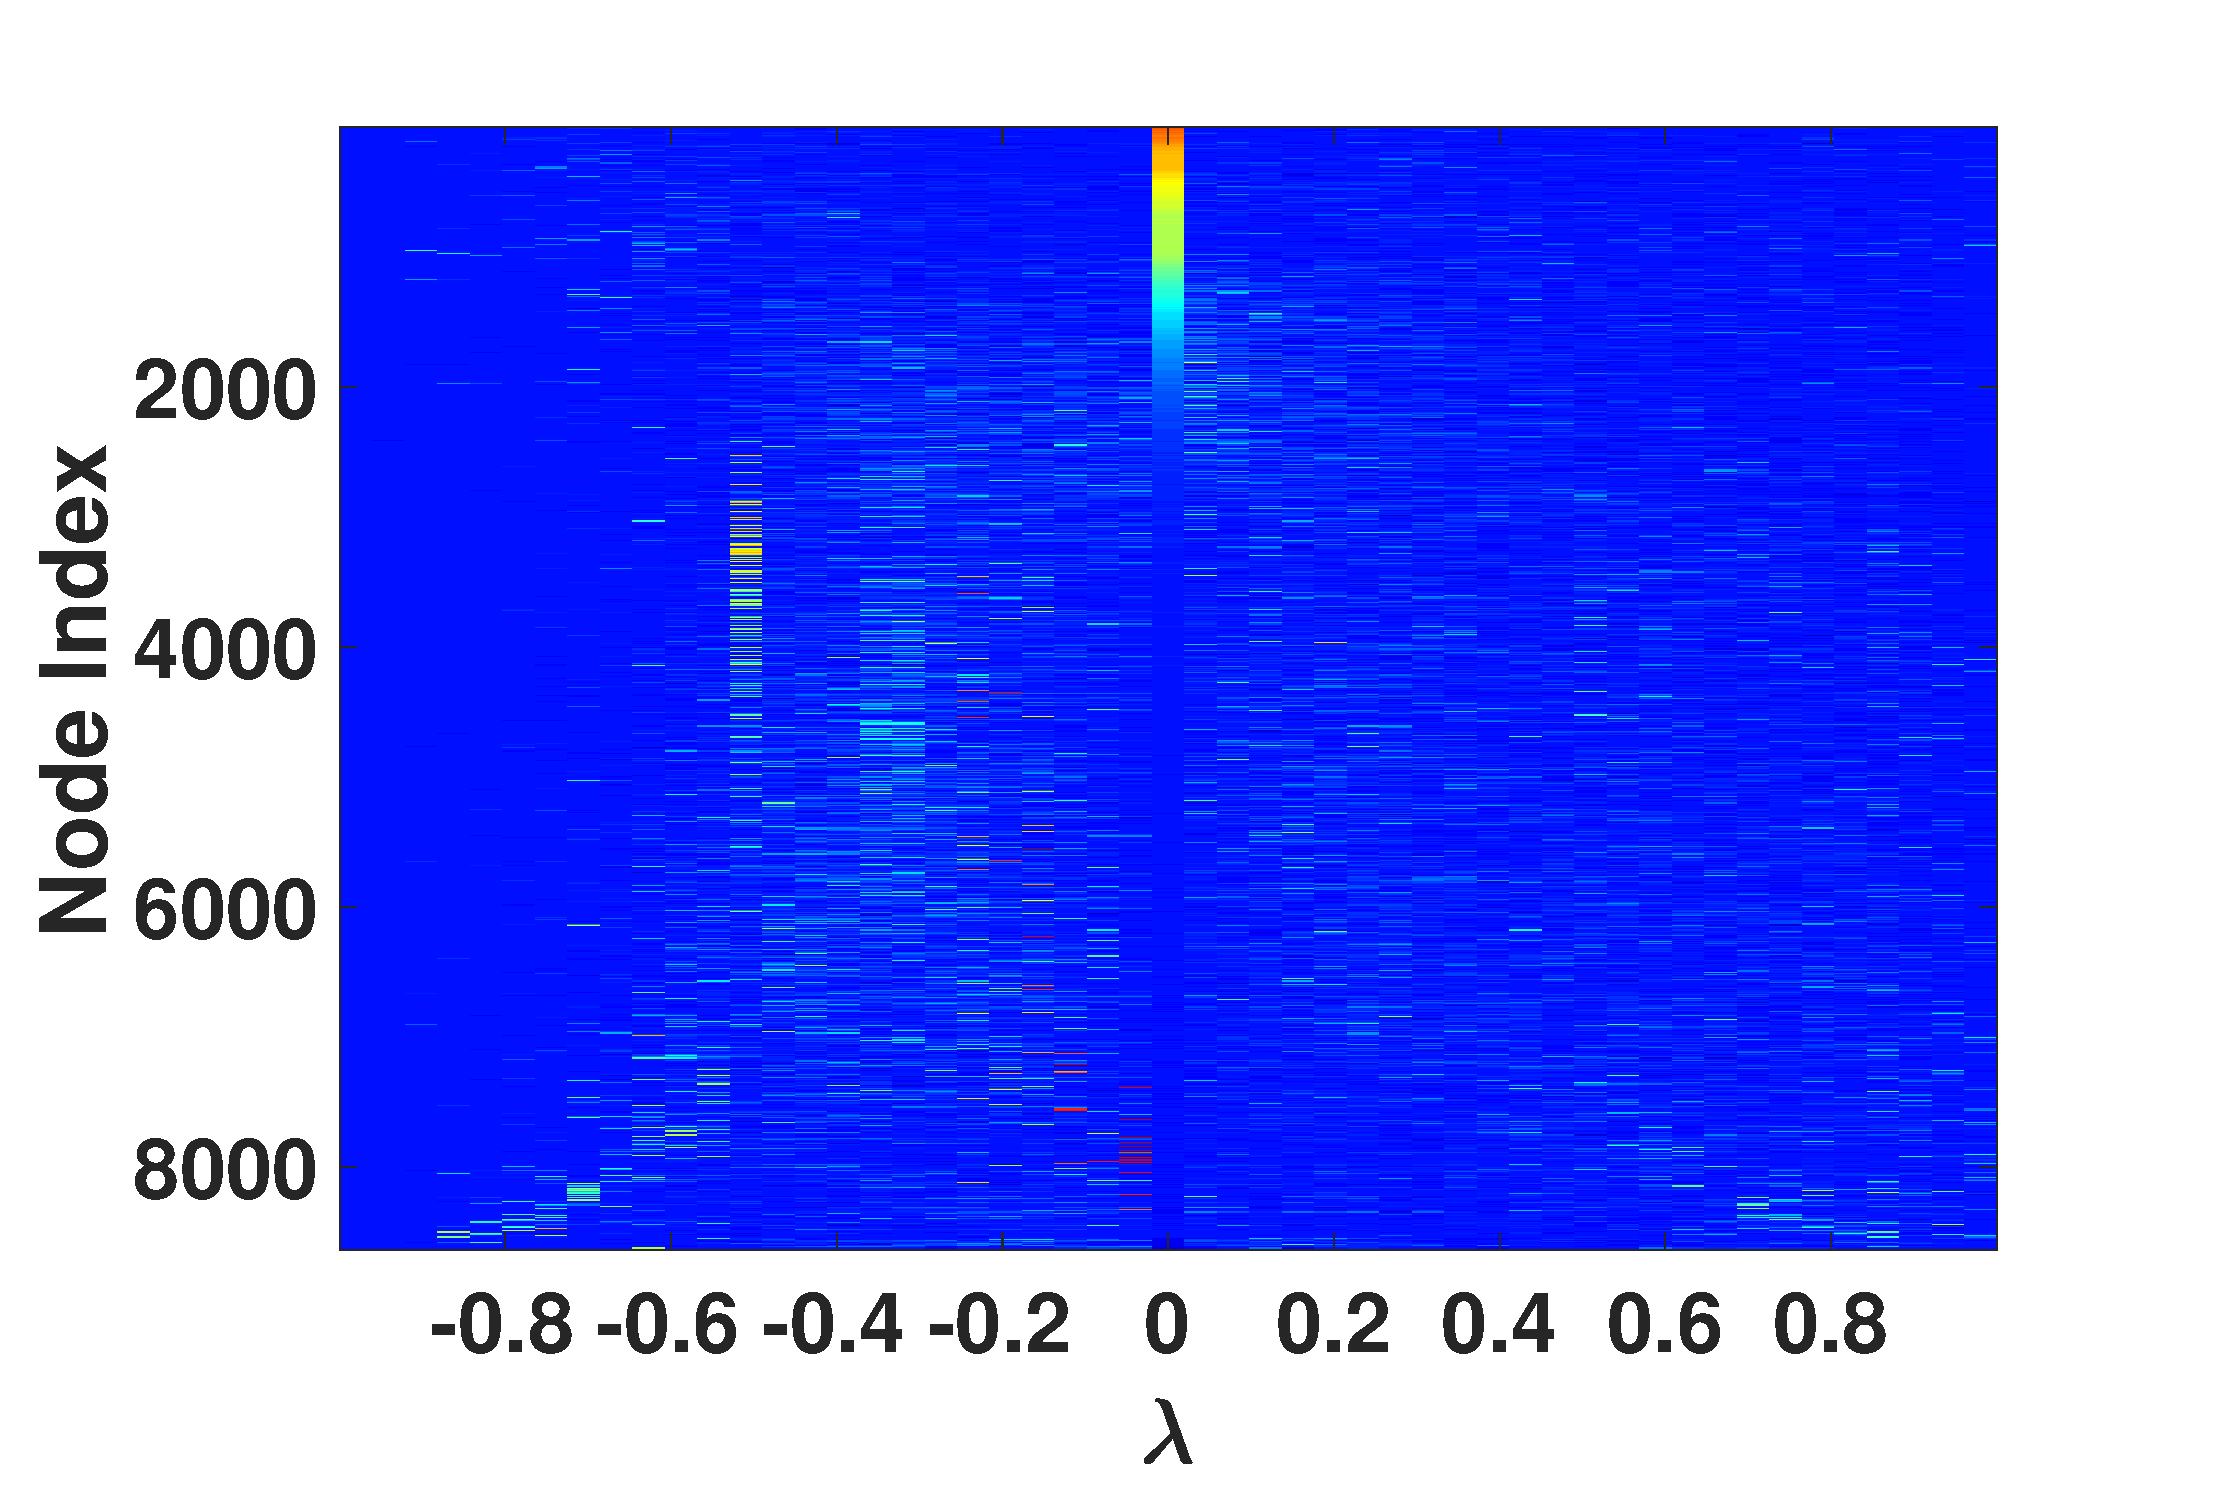
\includegraphics[width=\textwidth,trim = .4cm 0.5cm 3.5cm 1.3cm,clip]
    {./ndos/pics/hepth_ldos}
    \caption{HepTh Collaboration Network}
    \label{fig:hepth_ldos}
  \end{subfigure}
  %
  \begin{subfigure}[t]{0.19\textwidth}
    \centering  
    \captionsetup{justification=centering,font=scriptsize}
    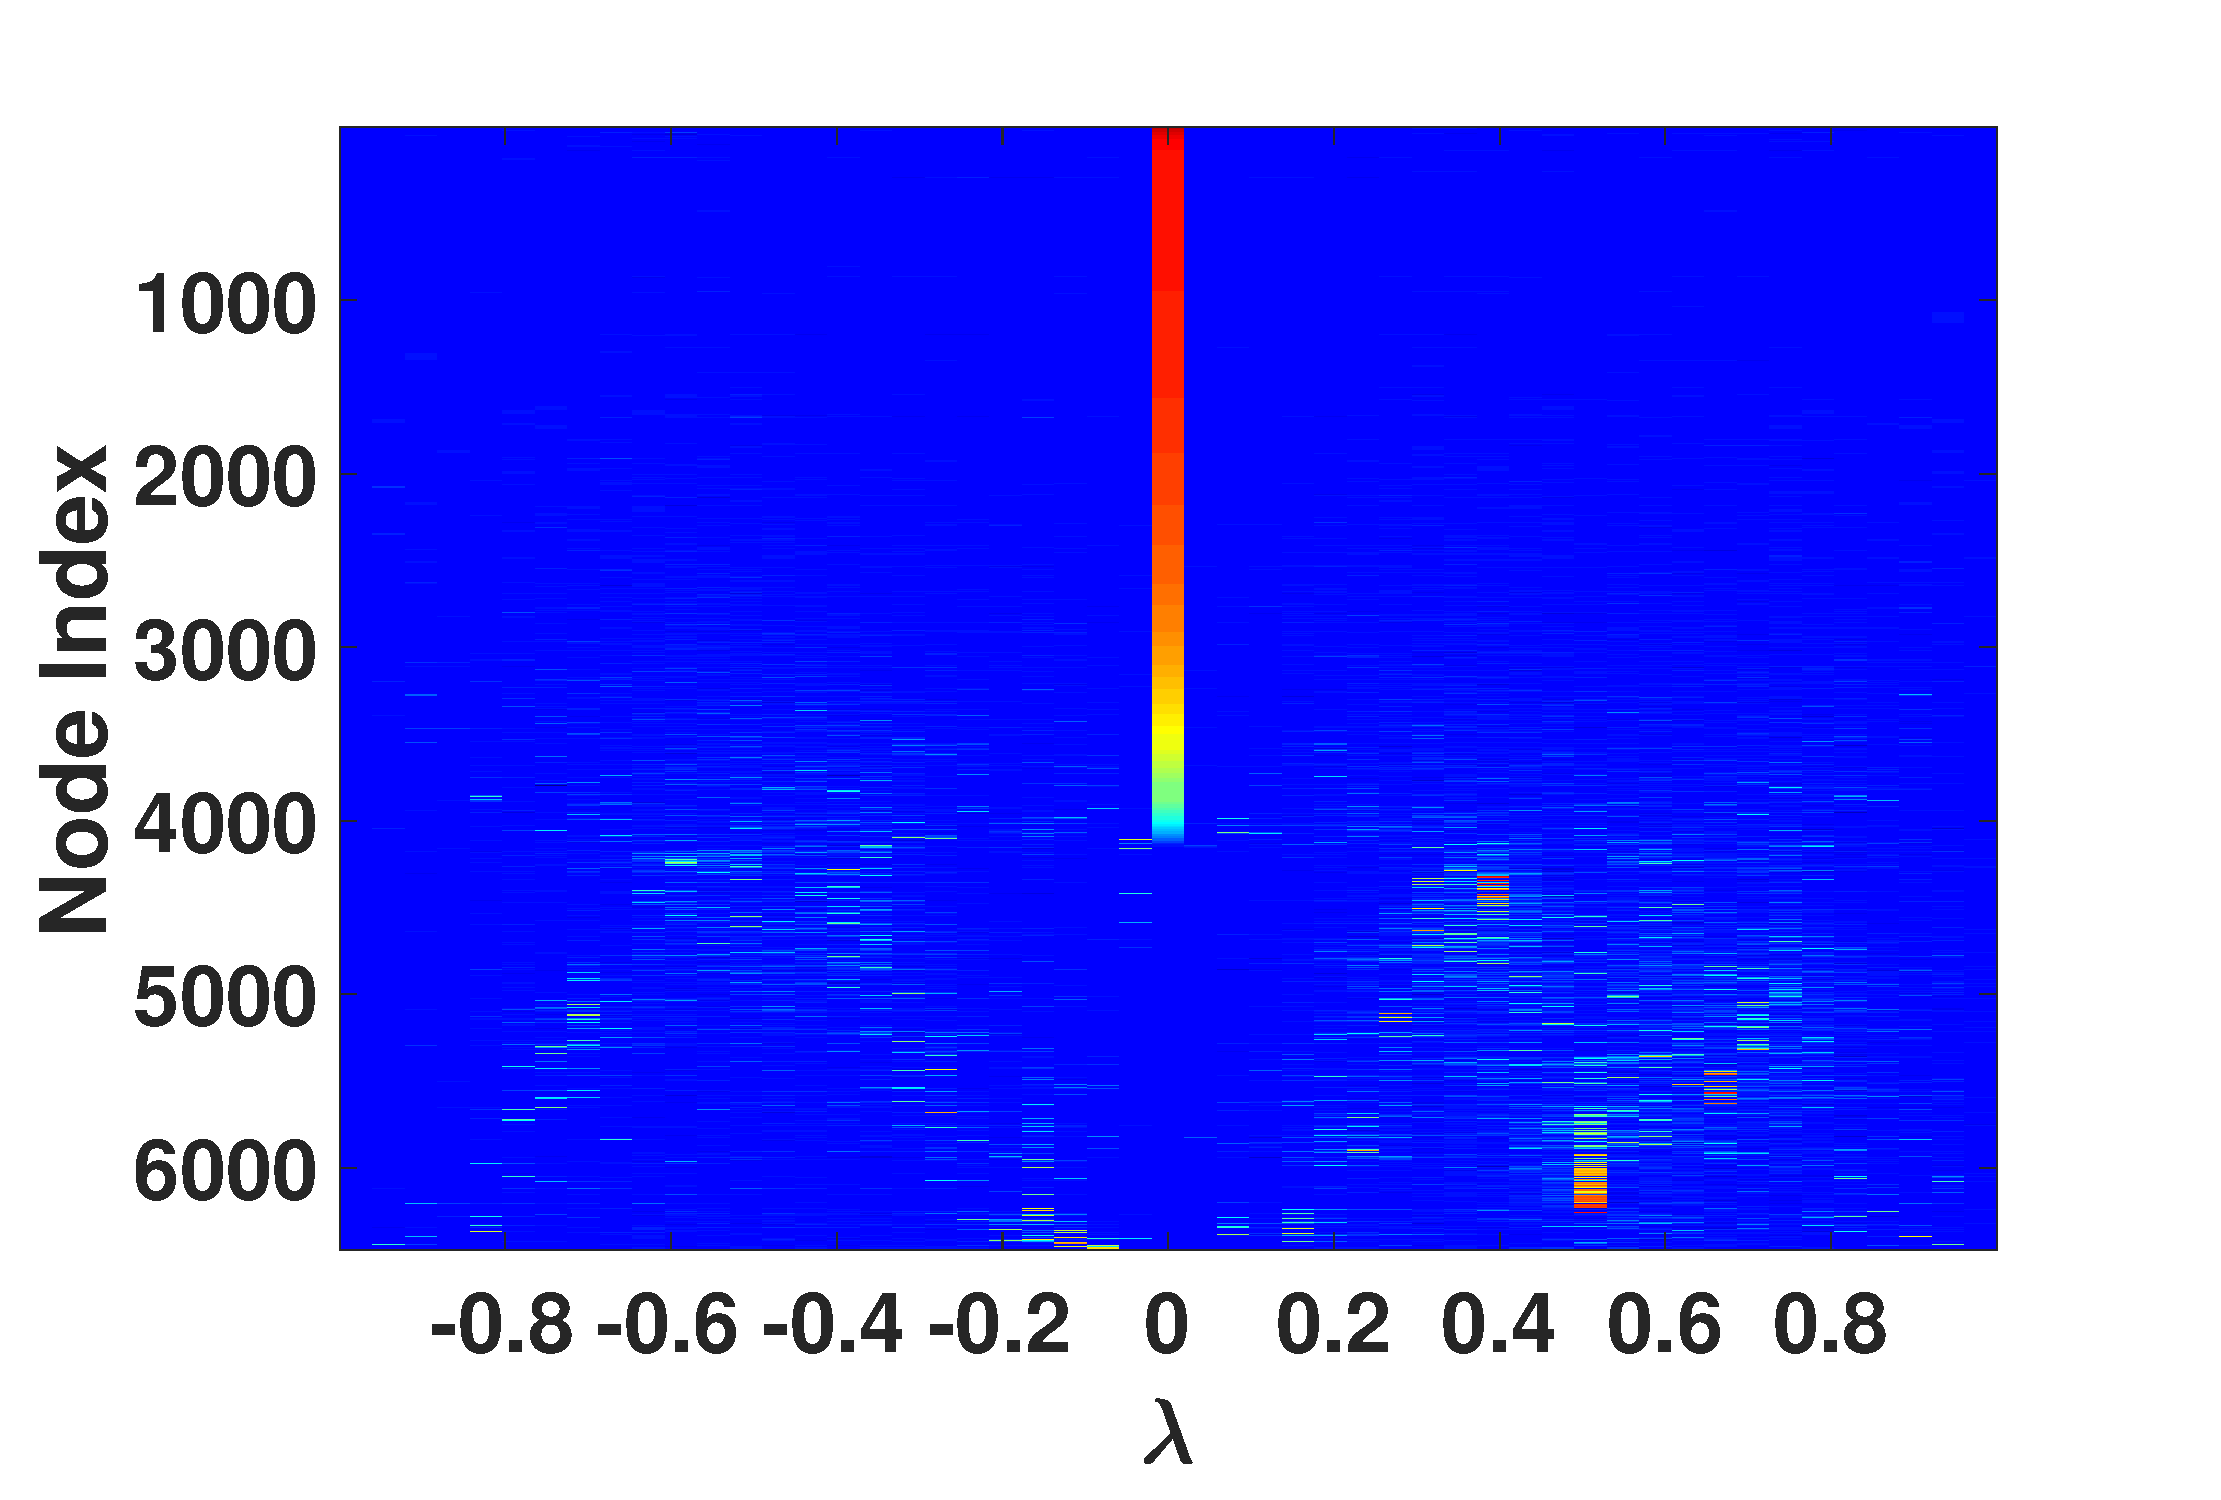
\includegraphics[width=\textwidth,trim = .4cm 0.5cm 3.5cm 1.3cm,clip]
    {./ndos/pics/as20000102_ldos}
    \caption{Autonomous System Network (2000)}
    \label{fig:as2_ldos}
  \end{subfigure}
  %
  \begin{subfigure}[t]{0.19\textwidth}
    \centering  
    \captionsetup{justification=centering,font=scriptsize}
    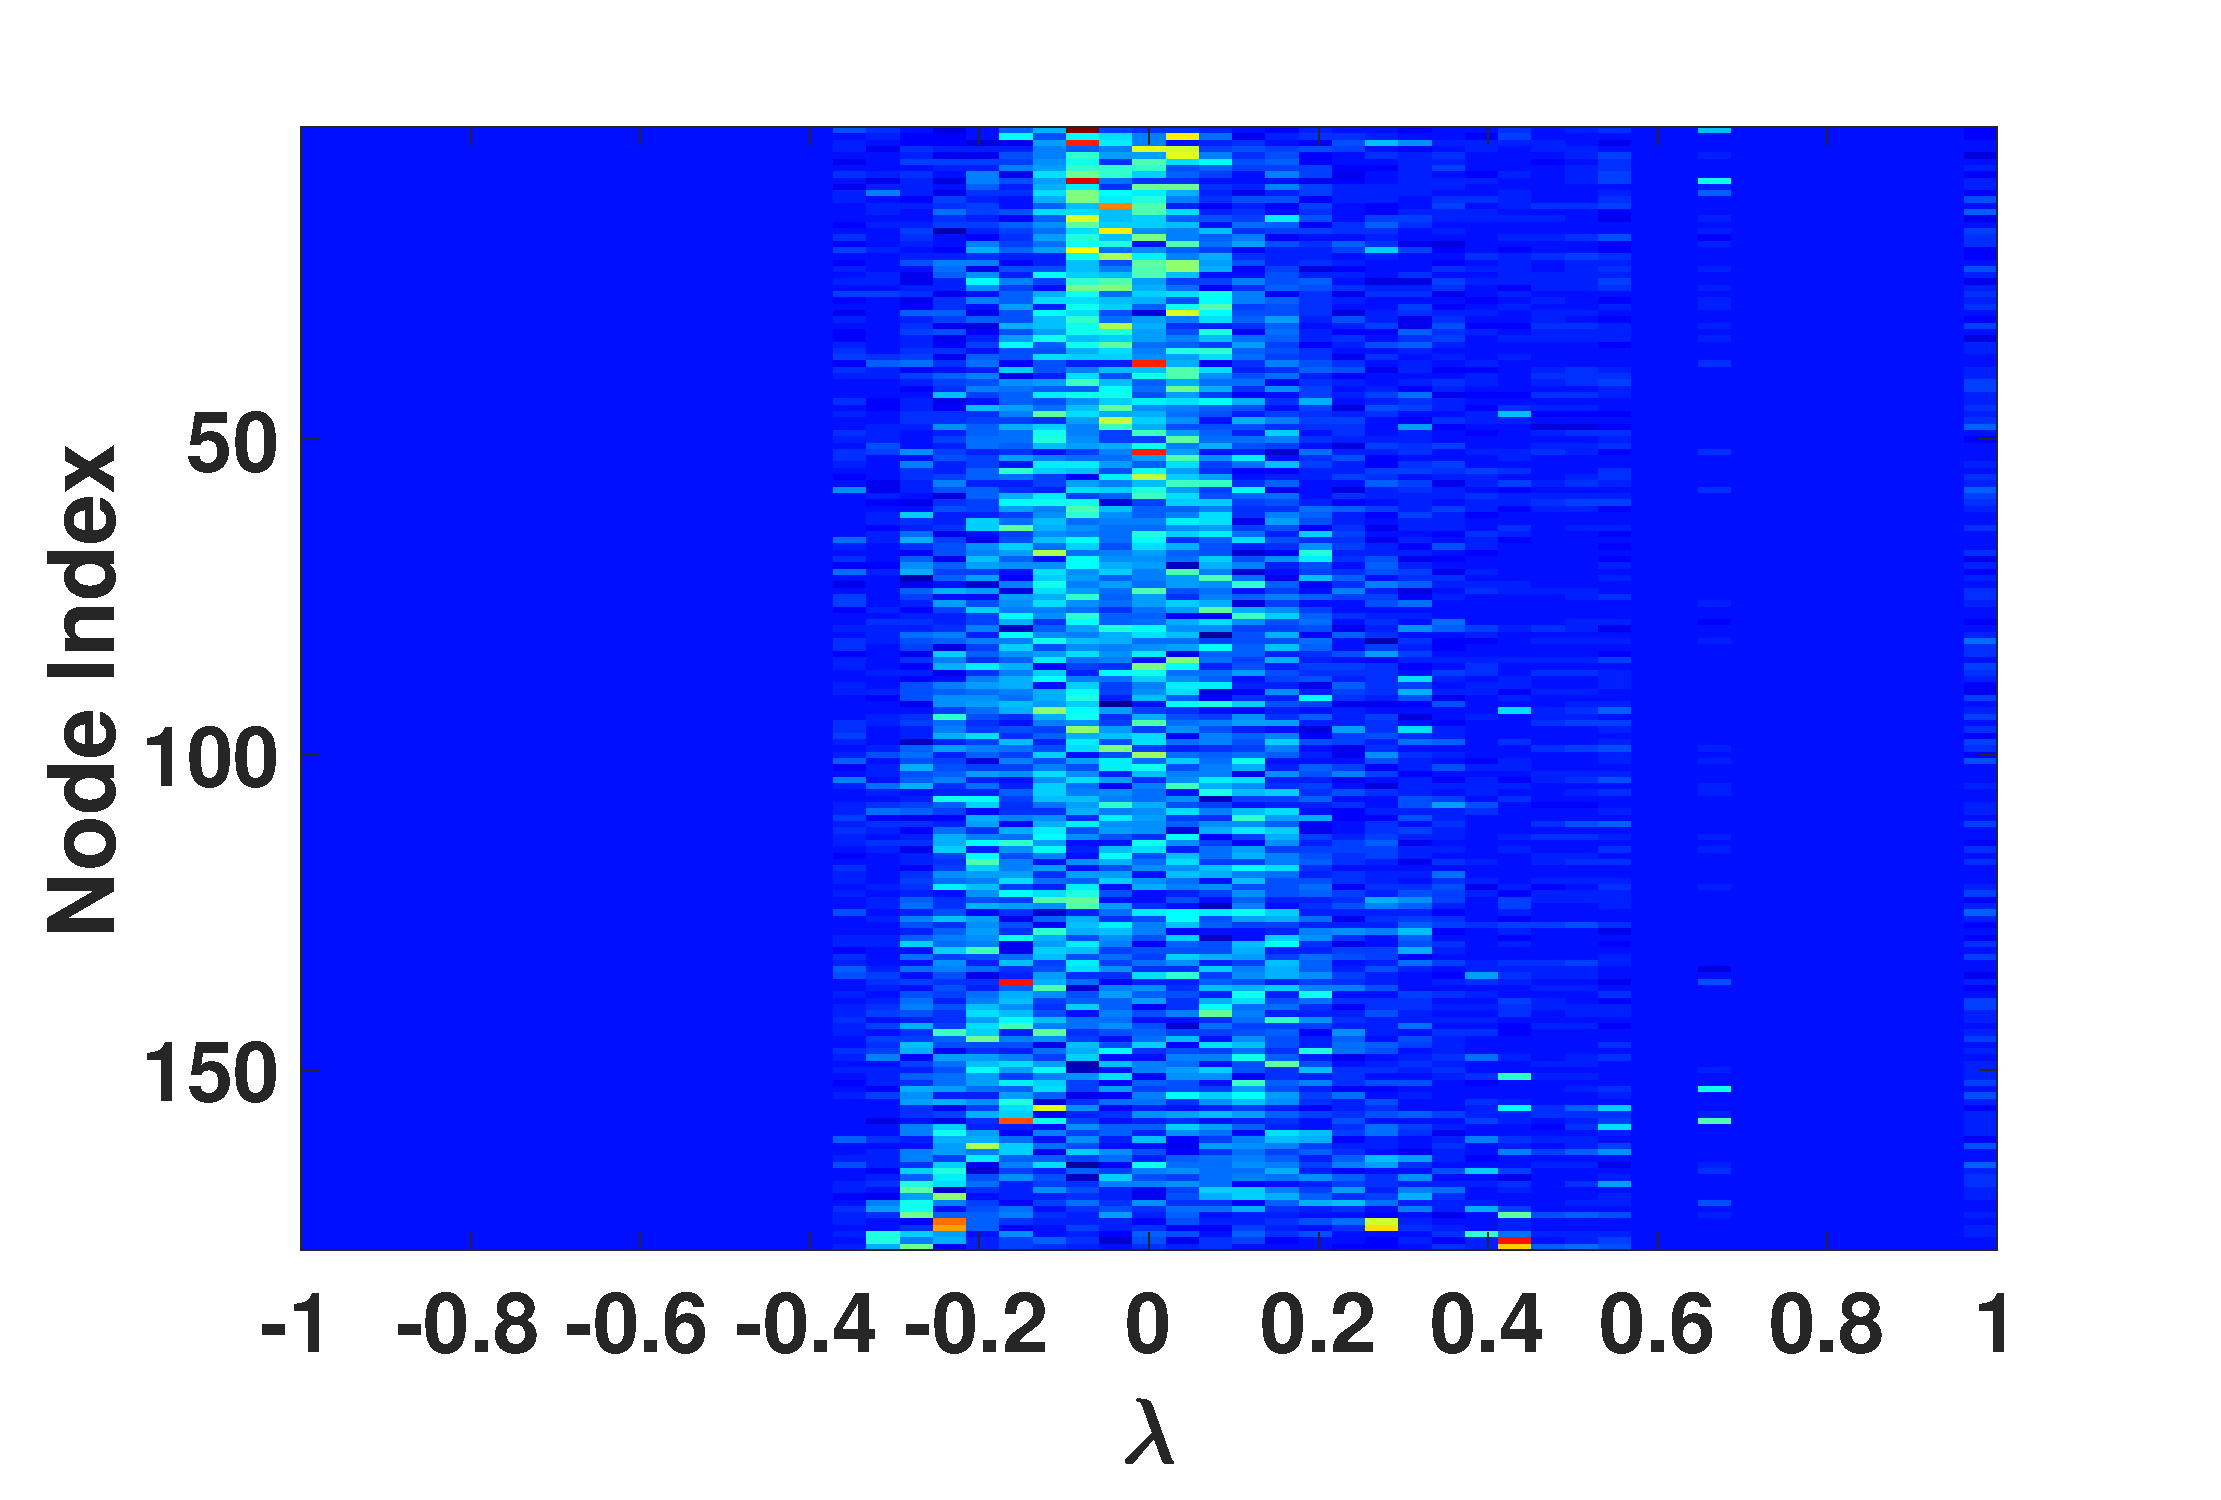
\includegraphics[width=\textwidth,trim = .4cm 0.5cm 3.5cm 1.3cm,clip]
    {./ndos/pics/hp_ldos}{}
    \caption{Harry Potter Characters Network}
    \label{fig:hp_ldos}
  \end{subfigure}
  %
  \begin{subfigure}[t]{0.19\textwidth}
    \centering  
    \captionsetup{justification=centering,font=scriptsize}
    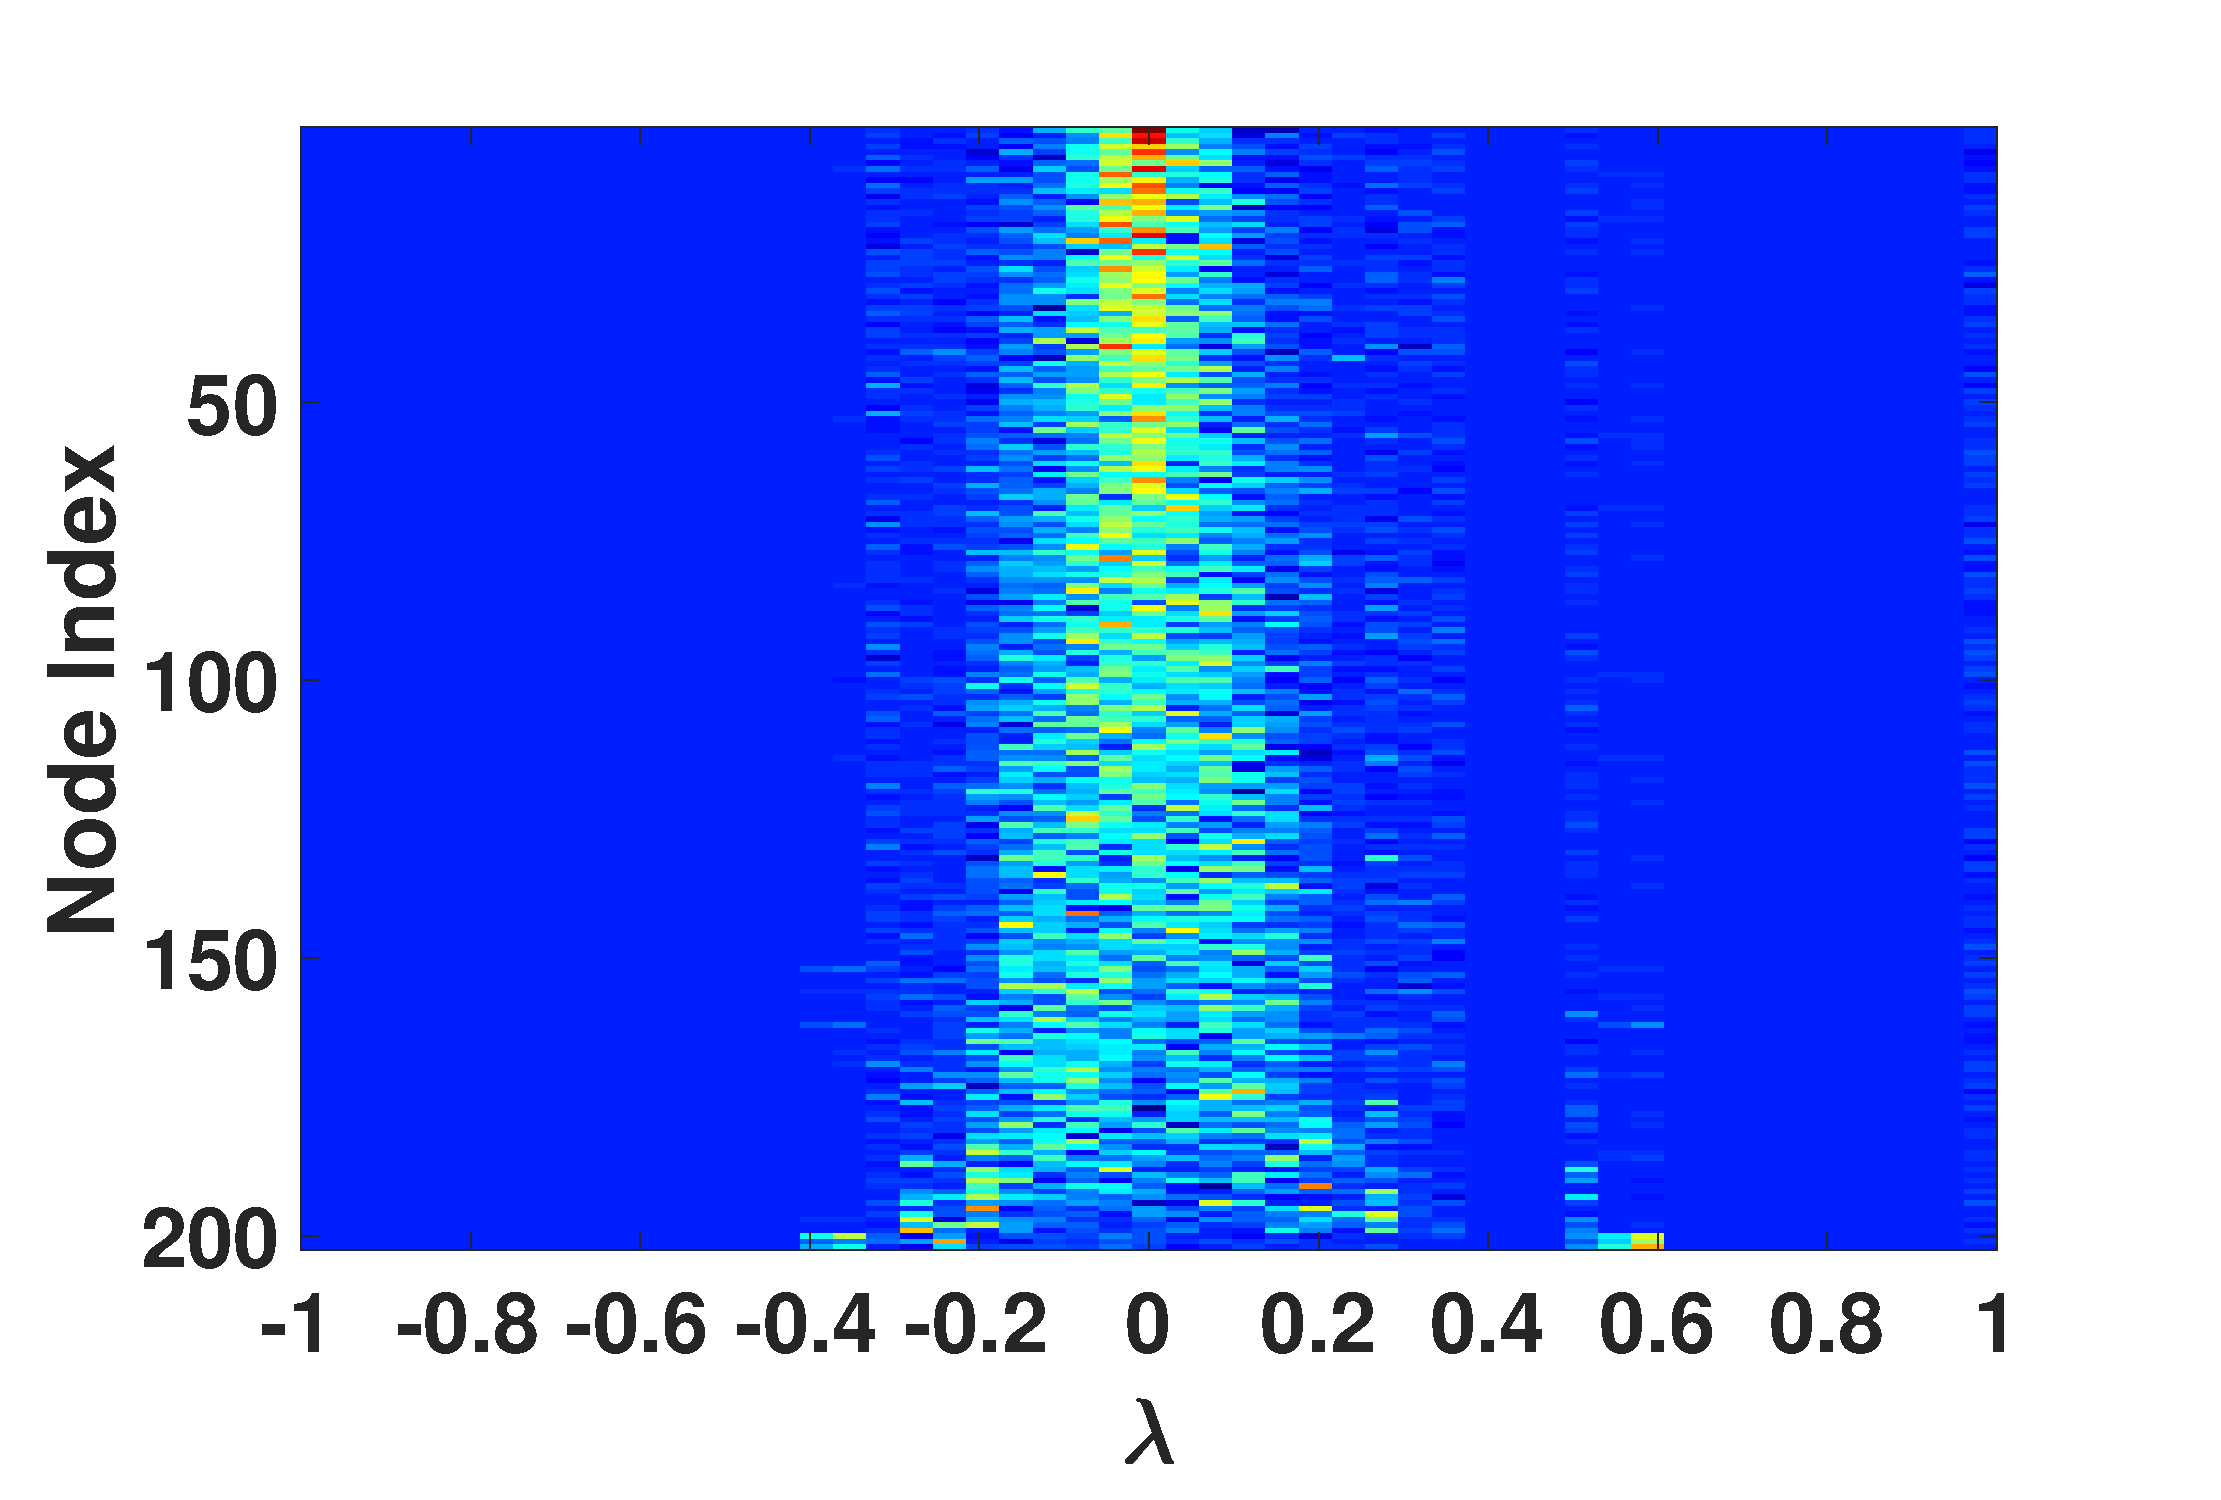
\includegraphics[width=\textwidth,trim = .4cm 0.5cm 3.5cm 1.3cm,clip]
    {./ndos/pics/twitter_ldos}
    \caption{Twitter Ego \\Networks}
    \label{fig:twitter_ldos}
  \end{subfigure}
  %
  \begin{subfigure}[t]{0.19\textwidth}
    \centering  
    \captionsetup{justification=centering,font=scriptsize}
    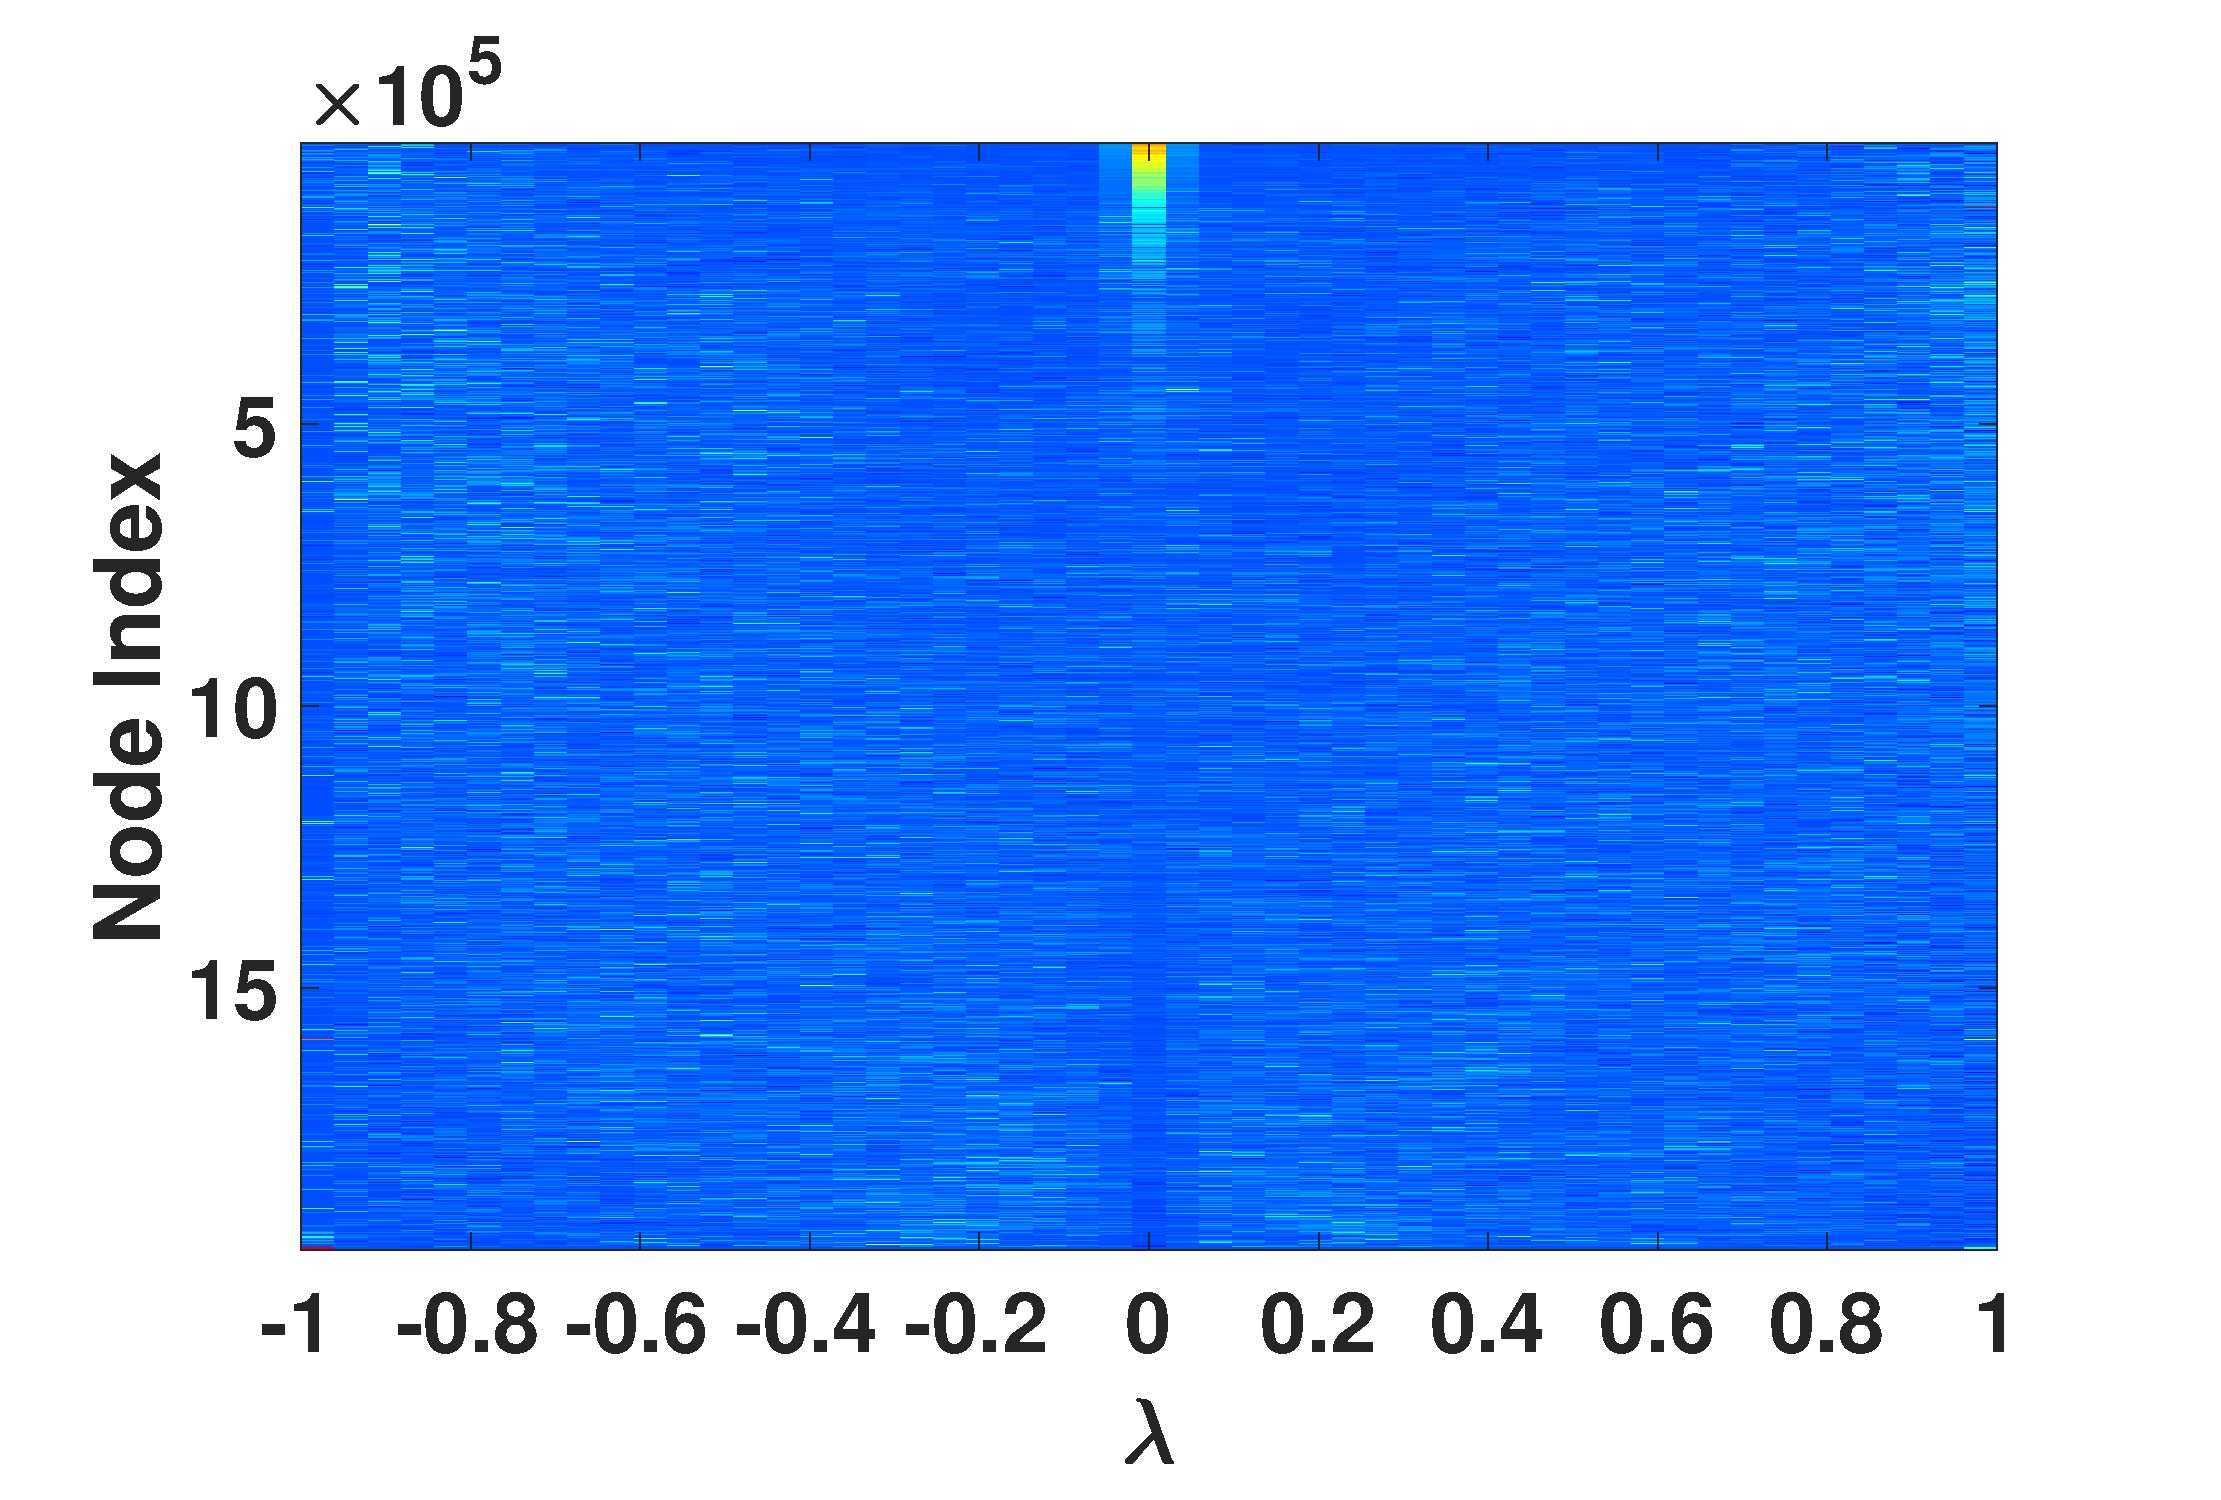
\includegraphics[width=\textwidth,trim = .4cm 0.5cm 3.5cm 0.3cm,clip]
    {./ndos/pics/roadca_ldos}
    \caption{California Road Network}
    \label{fig:roadca_ldos}
  \end{subfigure}
  \caption{DOS(top)/PDOS(bottom) histograms for the normalized adjacency of 10
  networks from five domains. For DOS, blue bars are the true spectrum, and red
  points are from KPM ($500$ moments and $20$ Hadamard probes). For PDOS, the
  spectral histograms of all nodes are aligned vertically. Red indicates high
  weight around an eigenvalue, and blue indicates low weight. The true spectrum
  for the California Road Network (\ref{fig:roadca_ldos}) is omitted, as it is
  too large to compute exactly (1,965,206 nodes).}\label{fig:gallery}
\end{figure}

\subsection{Computation time}

In this experiment, we show the scaling of our methods by applying them to
graphs of varying size of nodes, edges, and sparsity patterns. Rather than
computation power, the memory cost of loading a graph with 100M-1B edges is more
often the constraint. Hence, we report runtimes for a Python version on a Google
Cloud instance with 200GB memory and an Intel Xeon E5 v3 CPU at 2.30GHz.

The datasets we use are obtained from the SNAP repository~\cite{snapnets}. For
each graph, we compute the first $10$ Chebyshev moments using KPM with $20$
probe vectors. Most importantly, the cost for each moment is independent of the
total number of moments we compute. \cref{tab:scaling} reports number of
nodes, number of edges, average degree of nodes, and the average runtime for
computing each moment. We can observe that the runtime is in accordance with
the theoretical complexity $\calO(N_z(\abs{V} + \abs{E}))$. For the Friendster
social network with about 1.8 billion edges, computing each moment takes about
1000 seconds to compute, which means we could obtain a rough approximation to
its spectrum within a day. As the dominant cost is matrix-matrix multiplication
and we use several probe vectors, our approach has ample opportunity for
parallel computation.
\begin{table}[ht]
  \begin{center}
  \captionsetup{width=.8\textwidth}
  \caption{Average Computation Time per Chebyshev Moment for Graphs from the
  SNAP Repository\textsuperscript{$\alpha$}.}\label{tab:scaling}
  \begin{threeparttable}
    \begin{tabular}{r r r r r}
      \toprule
      Network & \# Nodes &\# Edges & Avg.\ Deg.\ & Time (s) \\ \midrule
      Facebook & 4,039 & 88,234 & 43.69 & 0.007\\
      AstroPh & 18,772 & 198,110 & 21.11 & 0.028\\
      Enron & 36,692 & 183,831 & 10.02 & 0.046\\
      Gplus & 107,614 & 13,673,453 & 254.12 & 1.133\\
      Amazon & 334,863 & 925,872 & 5.53 & 0.628\\
      Neuron & 1,018,524 & 24,735,503 & 48.57 & 9.138\\
      RoadNetCA & 1,965,206 & 2,766,607 & 2.82 & 2.276\\
      Orkut & 3,072,441 & 117,185,083 & 76.28 & 153.7\\
      LiveJournal & 3,997,962 & 34,681,189 & 17.35 & 14.52 \\
      Friendster & 65,608,366 & 1,806,067,135 & 55.06 & 1,017\\
      \bottomrule
    \end{tabular}
    \begin{tablenotes}
      \item[$\alpha$]$20$ probe vectors are used throughout the experiment. The
      runtime is averaged over 5 moments.
    \end{tablenotes}
  \end{threeparttable}
  \end{center}
\end{table}

\subsection{Model Verification}

In this experiment, we investigate the spectrum for some of the popular graph
models, and whether they resemble the behavior of real-world data. Two of the
most popular models used to describe real-world graphs are the scale-free model 
\cite{barabasi1999emergence} and the small-world model 
\cite{watts1998collective}. \citet{farkas2001spectra} has analyzed
the spectrum of the adjacency matrix; we instead consider the normalized
adjacency.

The scale-free model grows a random graph with the preferential attachment
process, starting from an initial seed graph and adding one node and $m$ edges
at every step. \cref{fig:ba} shows spectral histograms for this model with
$5000$ nodes and different choices of $m$. When $m=1$, the generated graph has
abundant local motifs like many sparse real-world graphs. By searching in PDOS
for the nodes that have high weight at the two spikes, we find node-doubles 
($\lambda=0)$ and singly-attached chains ($\lambda=\pm 1/\sqrt{2}$). When $m=5$,
the graph is denser, without any particular motifs, resulting in an
approximately semicircular spectral distribution.

\begin{figure}[ht]
  \begin{subfigure}{0.47\textwidth}
    \centering  
    \captionsetup{justification=centering}
    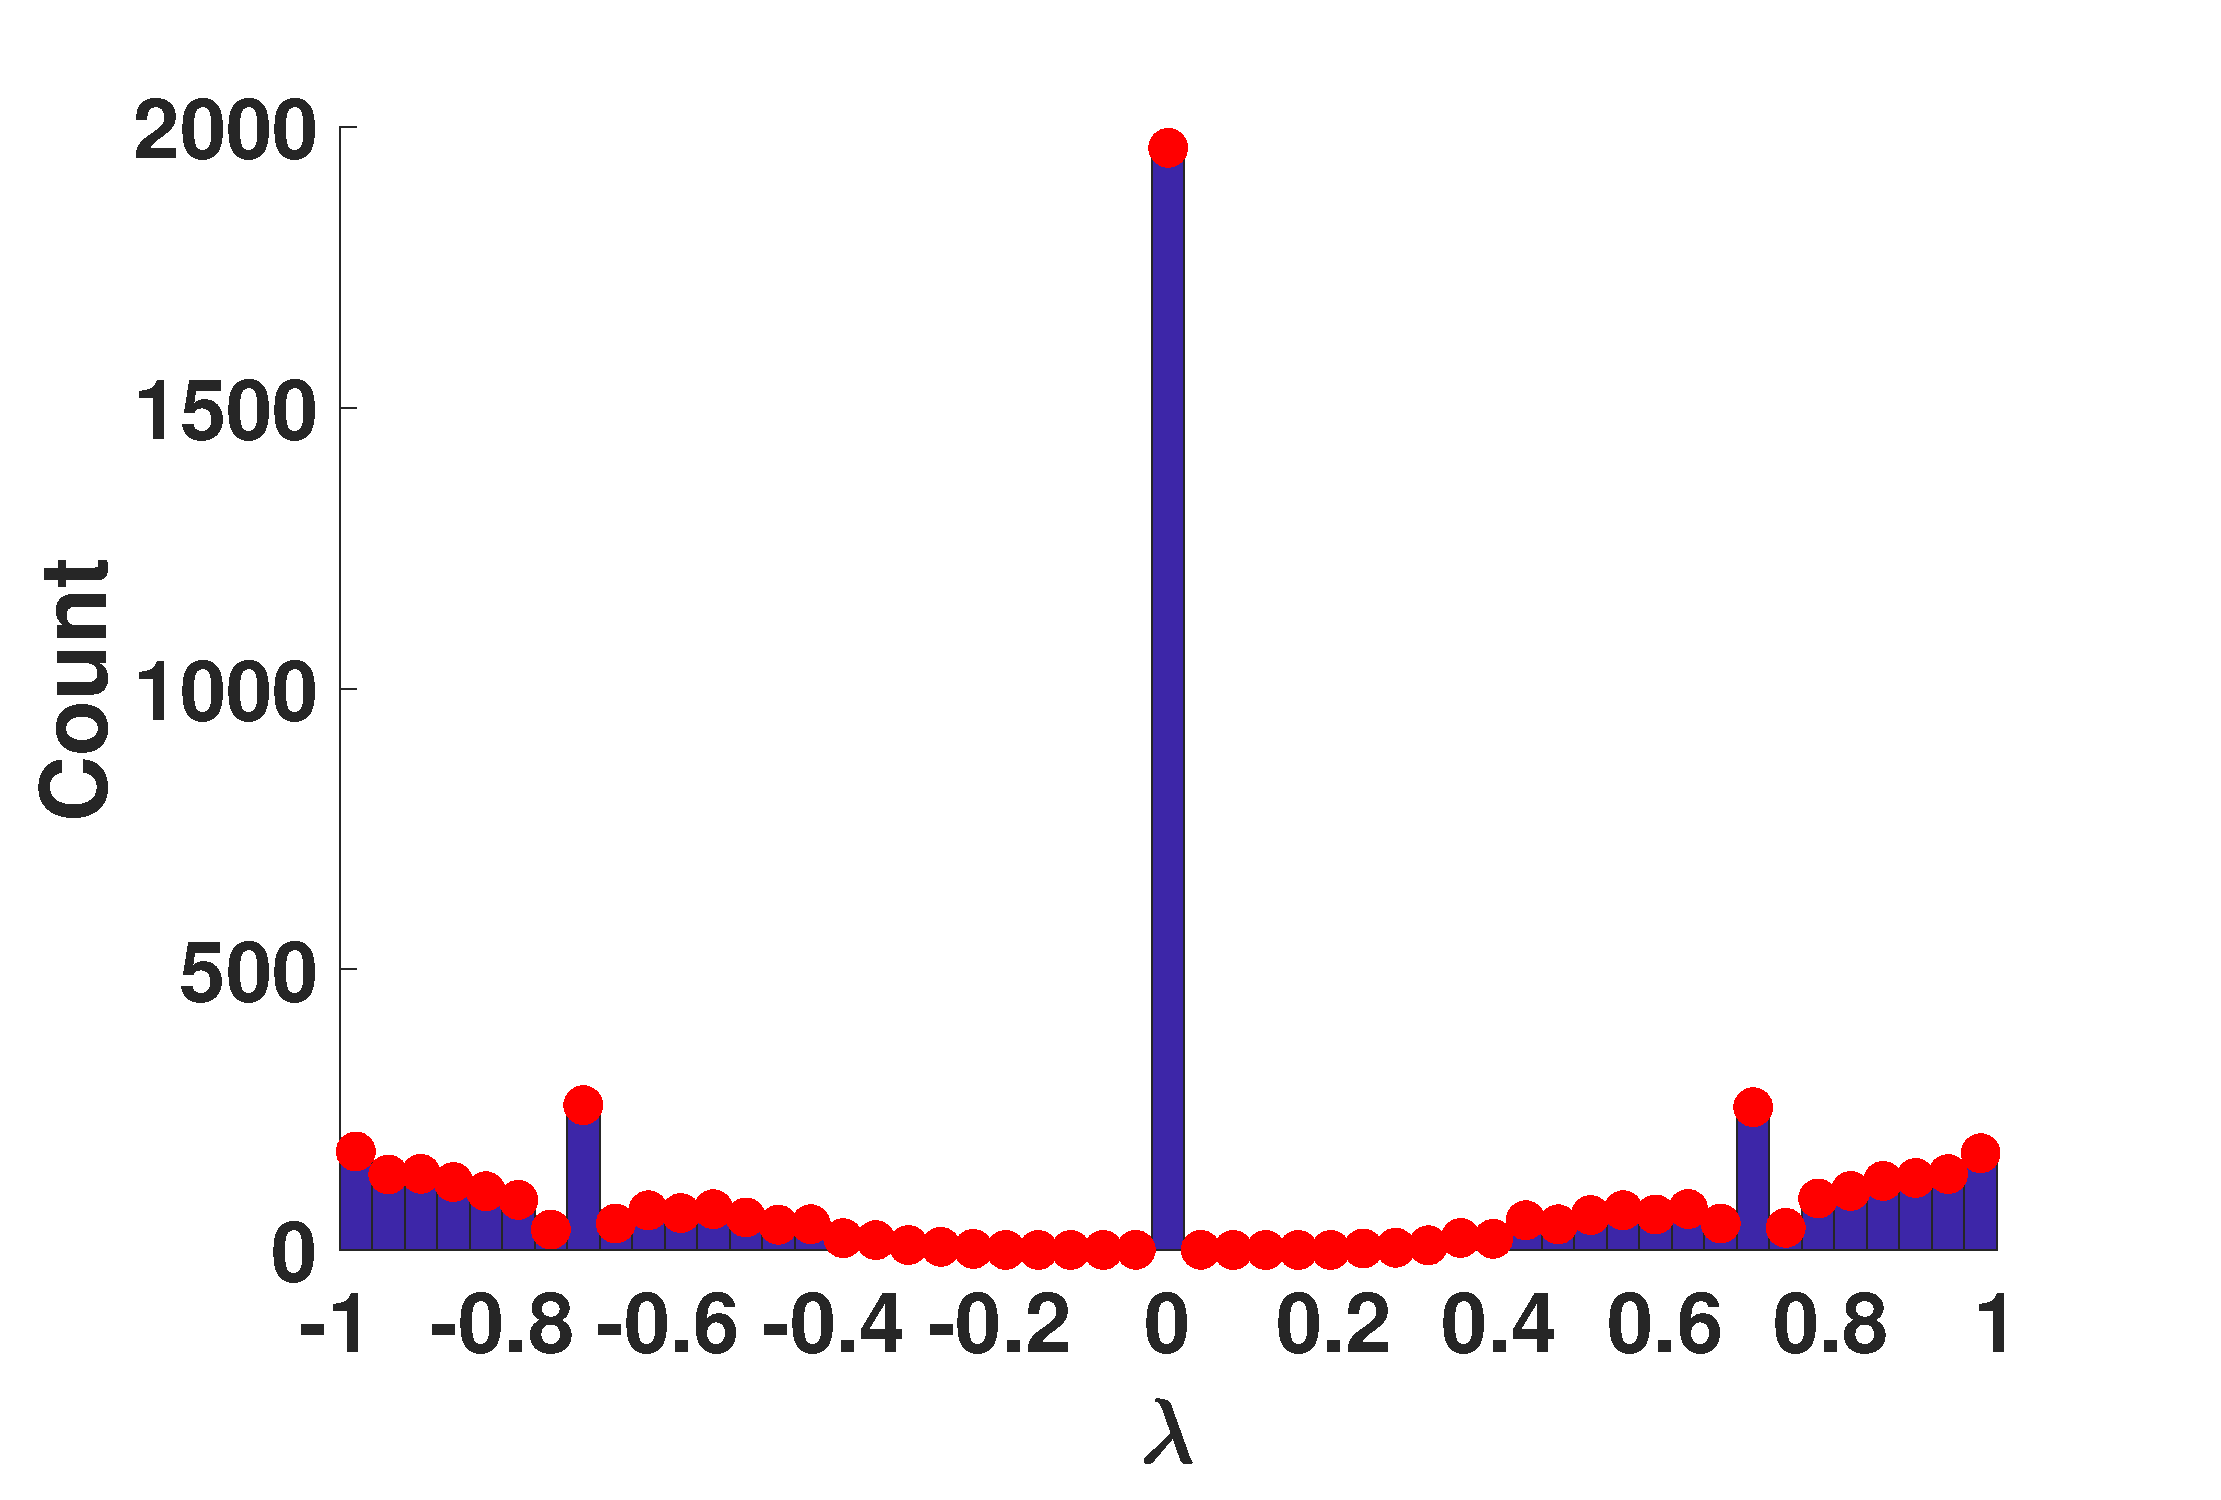
\includegraphics[width=\textwidth,trim = .4cm 0.5cm 3.5cm 1.3cm,clip]
    {./ndos/pics/ba_sparse}
    \caption{$m = 1$}\label{fig:ba_sparse}
  \end{subfigure}
  %
  \begin{subfigure}{0.47\textwidth}
    \centering
    \captionsetup{justification=centering}
    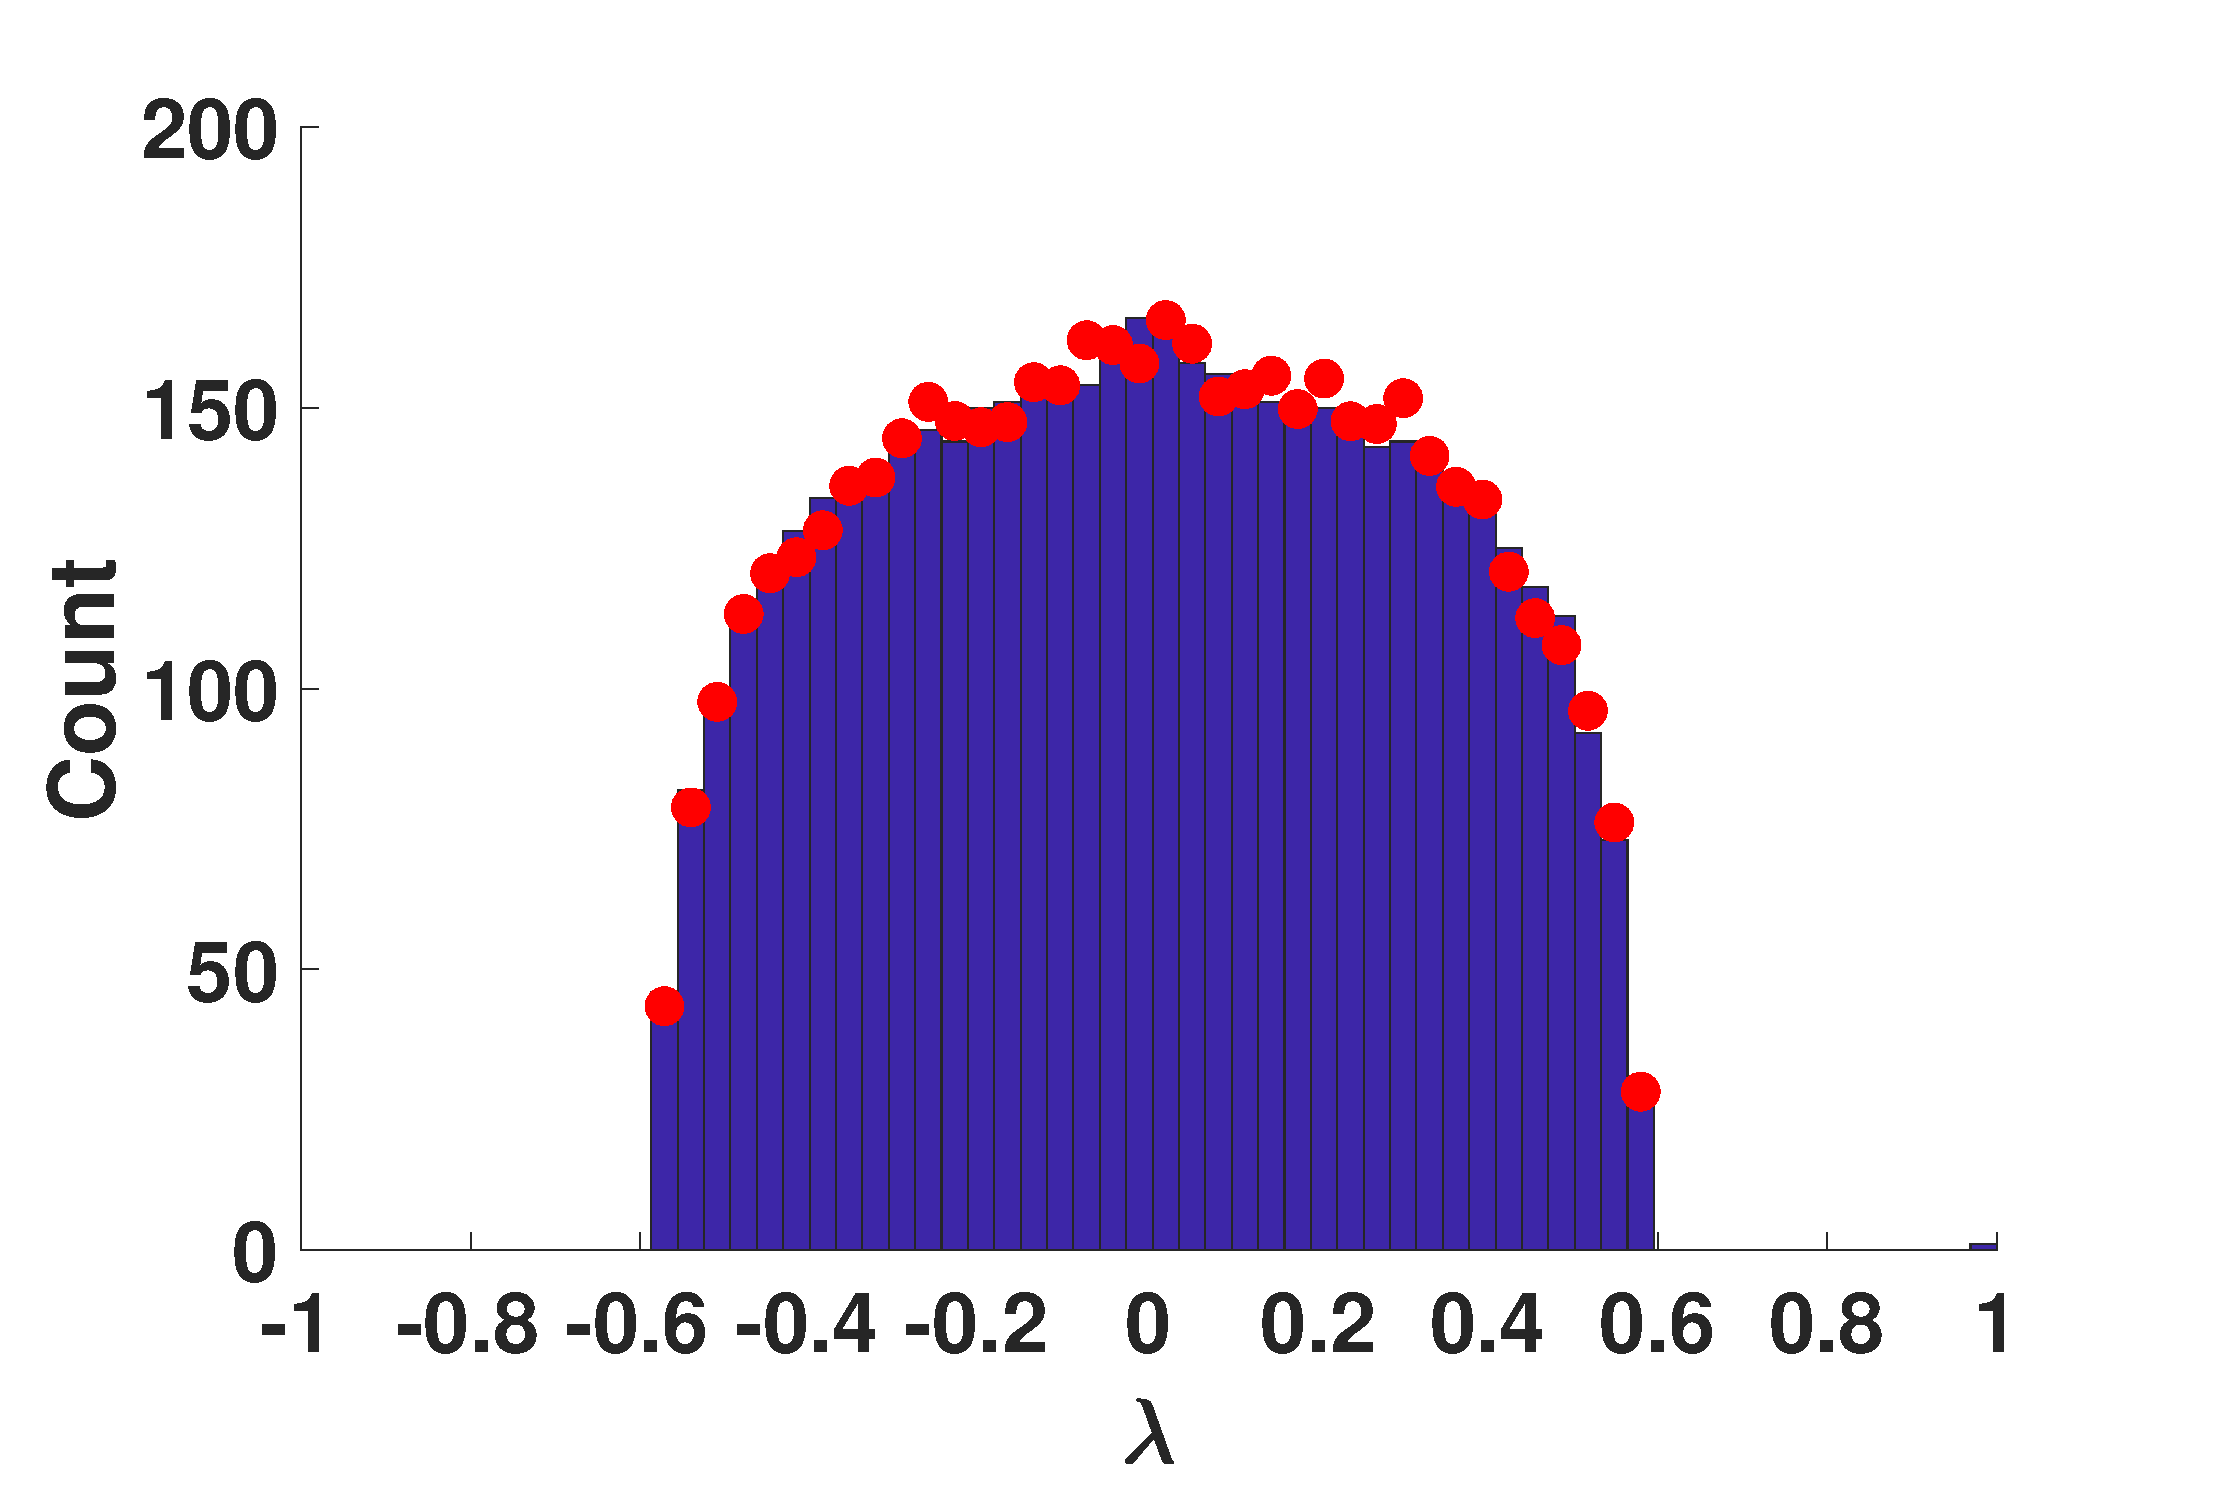
\includegraphics[width=\textwidth,trim = .4cm 0.5cm 3.5cm 1.3cm,clip]
    {./ndos/pics/ba_dense}
    \caption{$m = 5$}\label{fig:ba_dense}
  \end{subfigure}
  \caption{Spectral histogram for scale-free model with $5000$ nodes and
  different $m$. Blue bars are the real spectrum, red points are from KPM
  ($500$ moments and $20$ probes).} \label{fig:ba}
\end{figure}

The small-world model generates a random graph by re-wiring edges of a ring
lattice with a certain probability $p$. Here we construct these graphs on $5000$
nodes with $p=0.5$; the pattern in spectrum is insensitive for a wide range of
$p$. In \cref{fig:sw}, when the graph is sparse with $5000$ edges, the spectrum
has spikes at $0$ and $\pm 1$, indicating local symmetries, bipartite structure,
and disconnected components. With $50000$ edges, localized structures disappear
and the spectrum has narrower support.

\begin{figure}[ht]
  \begin{subfigure}{0.47\textwidth}
    \centering  
    \captionsetup{justification=centering}
    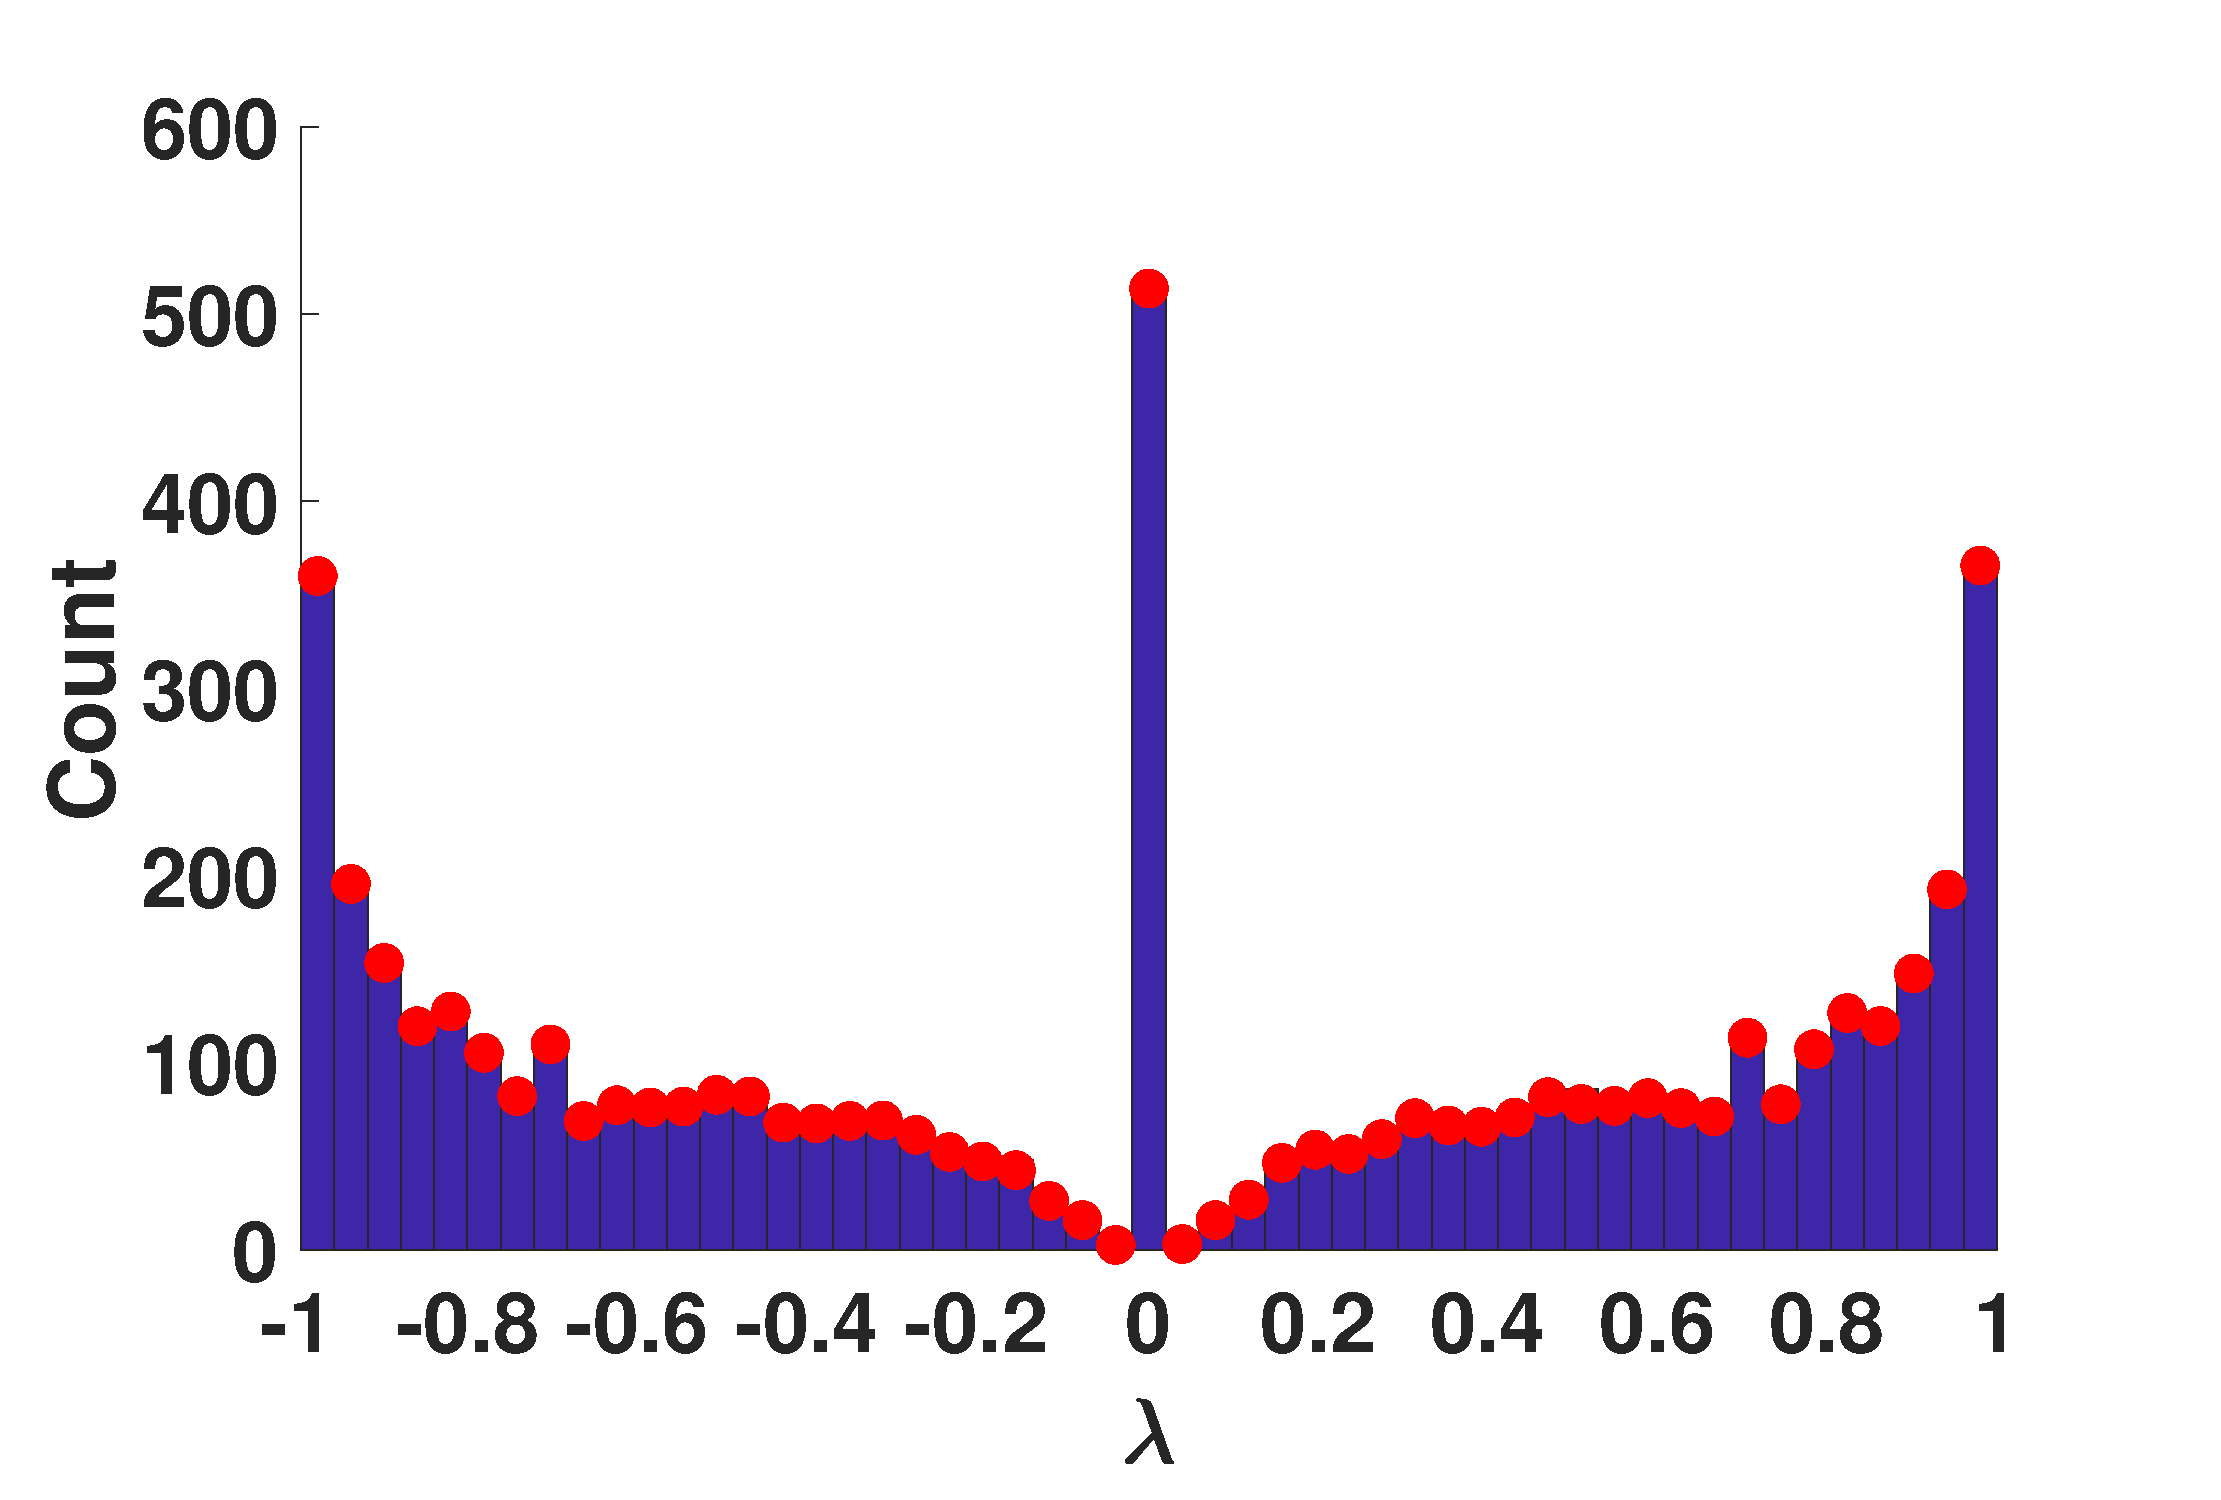
\includegraphics[width=\textwidth,trim = .4cm 0.5cm 3.5cm 1.3cm,clip]
    {./ndos/pics/sw_sparse}
    \caption{$\abs{E}=5k$}\label{fig:sw_sparse}
  \end{subfigure}
  %
  \begin{subfigure}{0.47\textwidth}
    \centering
    \captionsetup{justification=centering}
    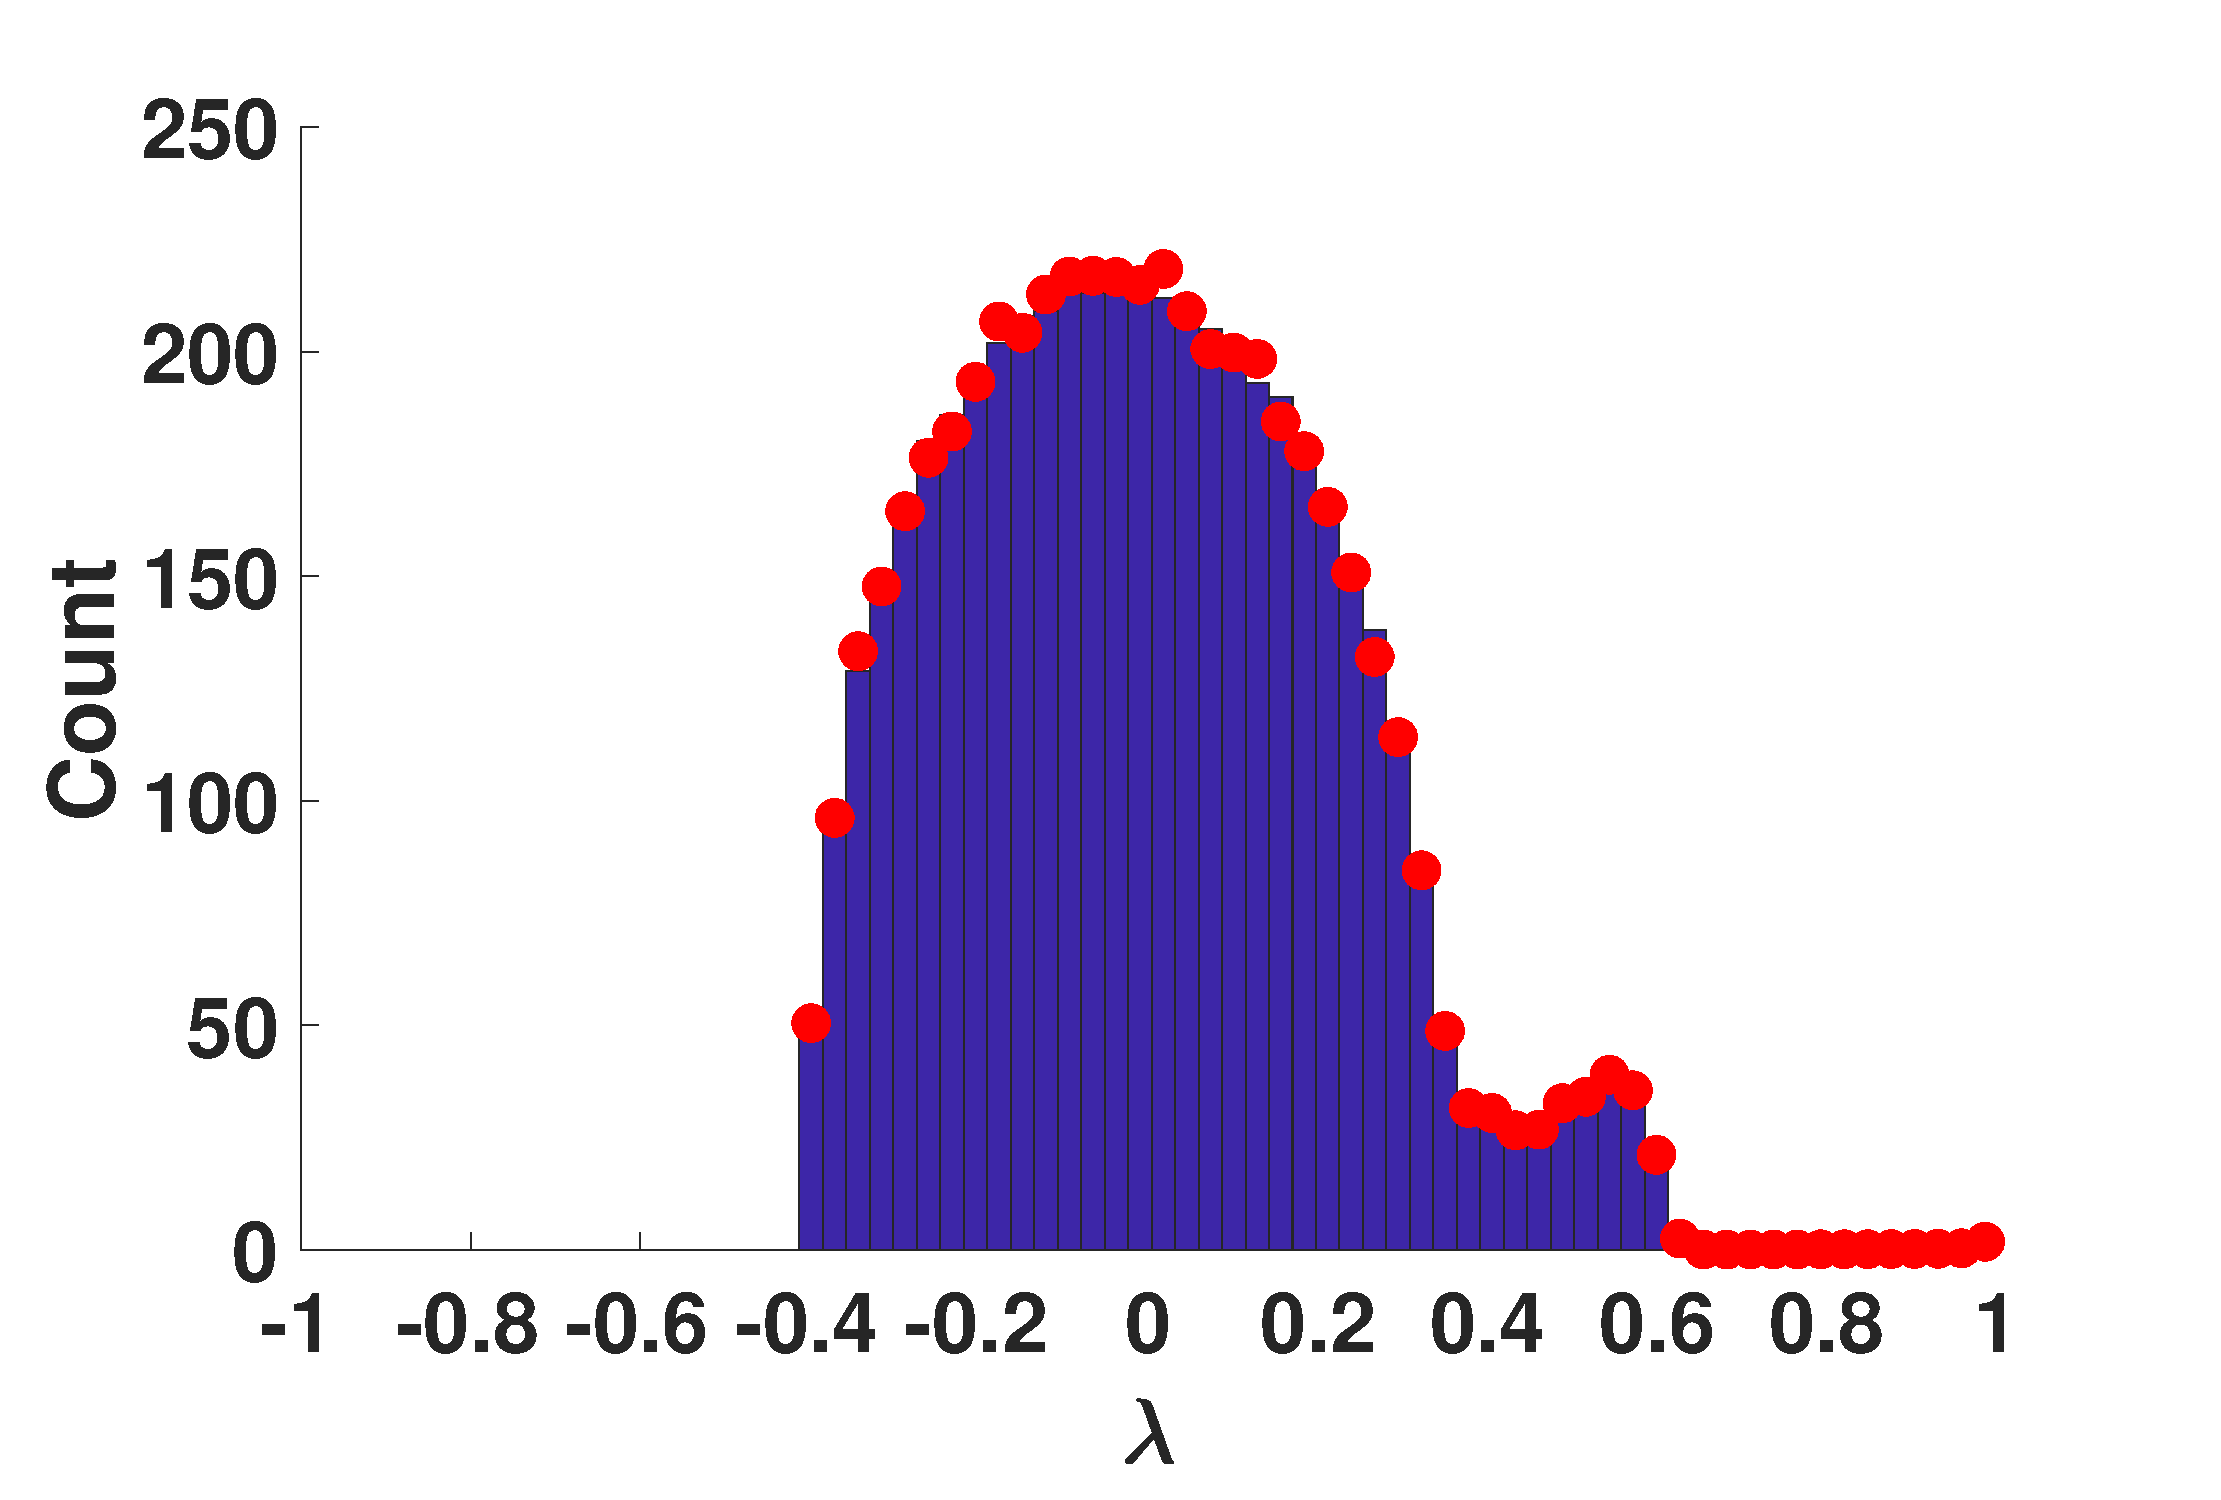
\includegraphics[width=\textwidth,trim = .4cm 0.5cm 3.5cm 1.3cm,clip]
    {./ndos/pics/sw_dense}
    \caption{$\abs{E}=50k$}\label{fig:sw_dense}
  \end{subfigure}
  \caption{Spectral histograms for small-world model with $5000$ nodes and
  re-wiring probability $p=0.5$, starting with $5000$ (\ref{fig:sw_sparse}) and
  $50000$ (\ref{fig:sw_dense} edges. Blue bars are the real spectrum, red points
  are from KPM ($5000$ moments and $20$ probes).} \label{fig:sw}
\end{figure}

Finally, we investigate the Block Two-Level \ErdosRenyi\ (BTER) model 
\cite{seshadhri2012community}, which directly fits an input graph. BTER
constructs a similar graph by a two-step process: first create a collection of
\ErdosRenyi\ subgraphs, then interconnect those using a Chung-Lu model  
\cite{chung2002connected}. \citeauthor{seshadhri2012community} showed their
model accurately captures the observable properties of the given graph,
including the eigenvalues of the adjacency matrix. \cref{fig:bter} compares the
DOS/PDOS of the Erd\"{o}s collaboration network and its BTER counterpart. Unlike
the original graph, most $0$ eigenvalues in BTER graph come from isolated nodes.
The BTER graph also has many more isolated edges ($\lambda=\pm1$),
singly-attached chains ($\lambda=\pm1/\sqrt{2})$), and singly-attached triangles
($\lambda=-1/2$). We locate these motifs by inspecting nodes with high weights
at respective part of the spectrum.

\begin{figure}[ht]
  \begin{subfigure}[t]{0.47\textwidth}
    \centering  
    \captionsetup{justification=centering}
    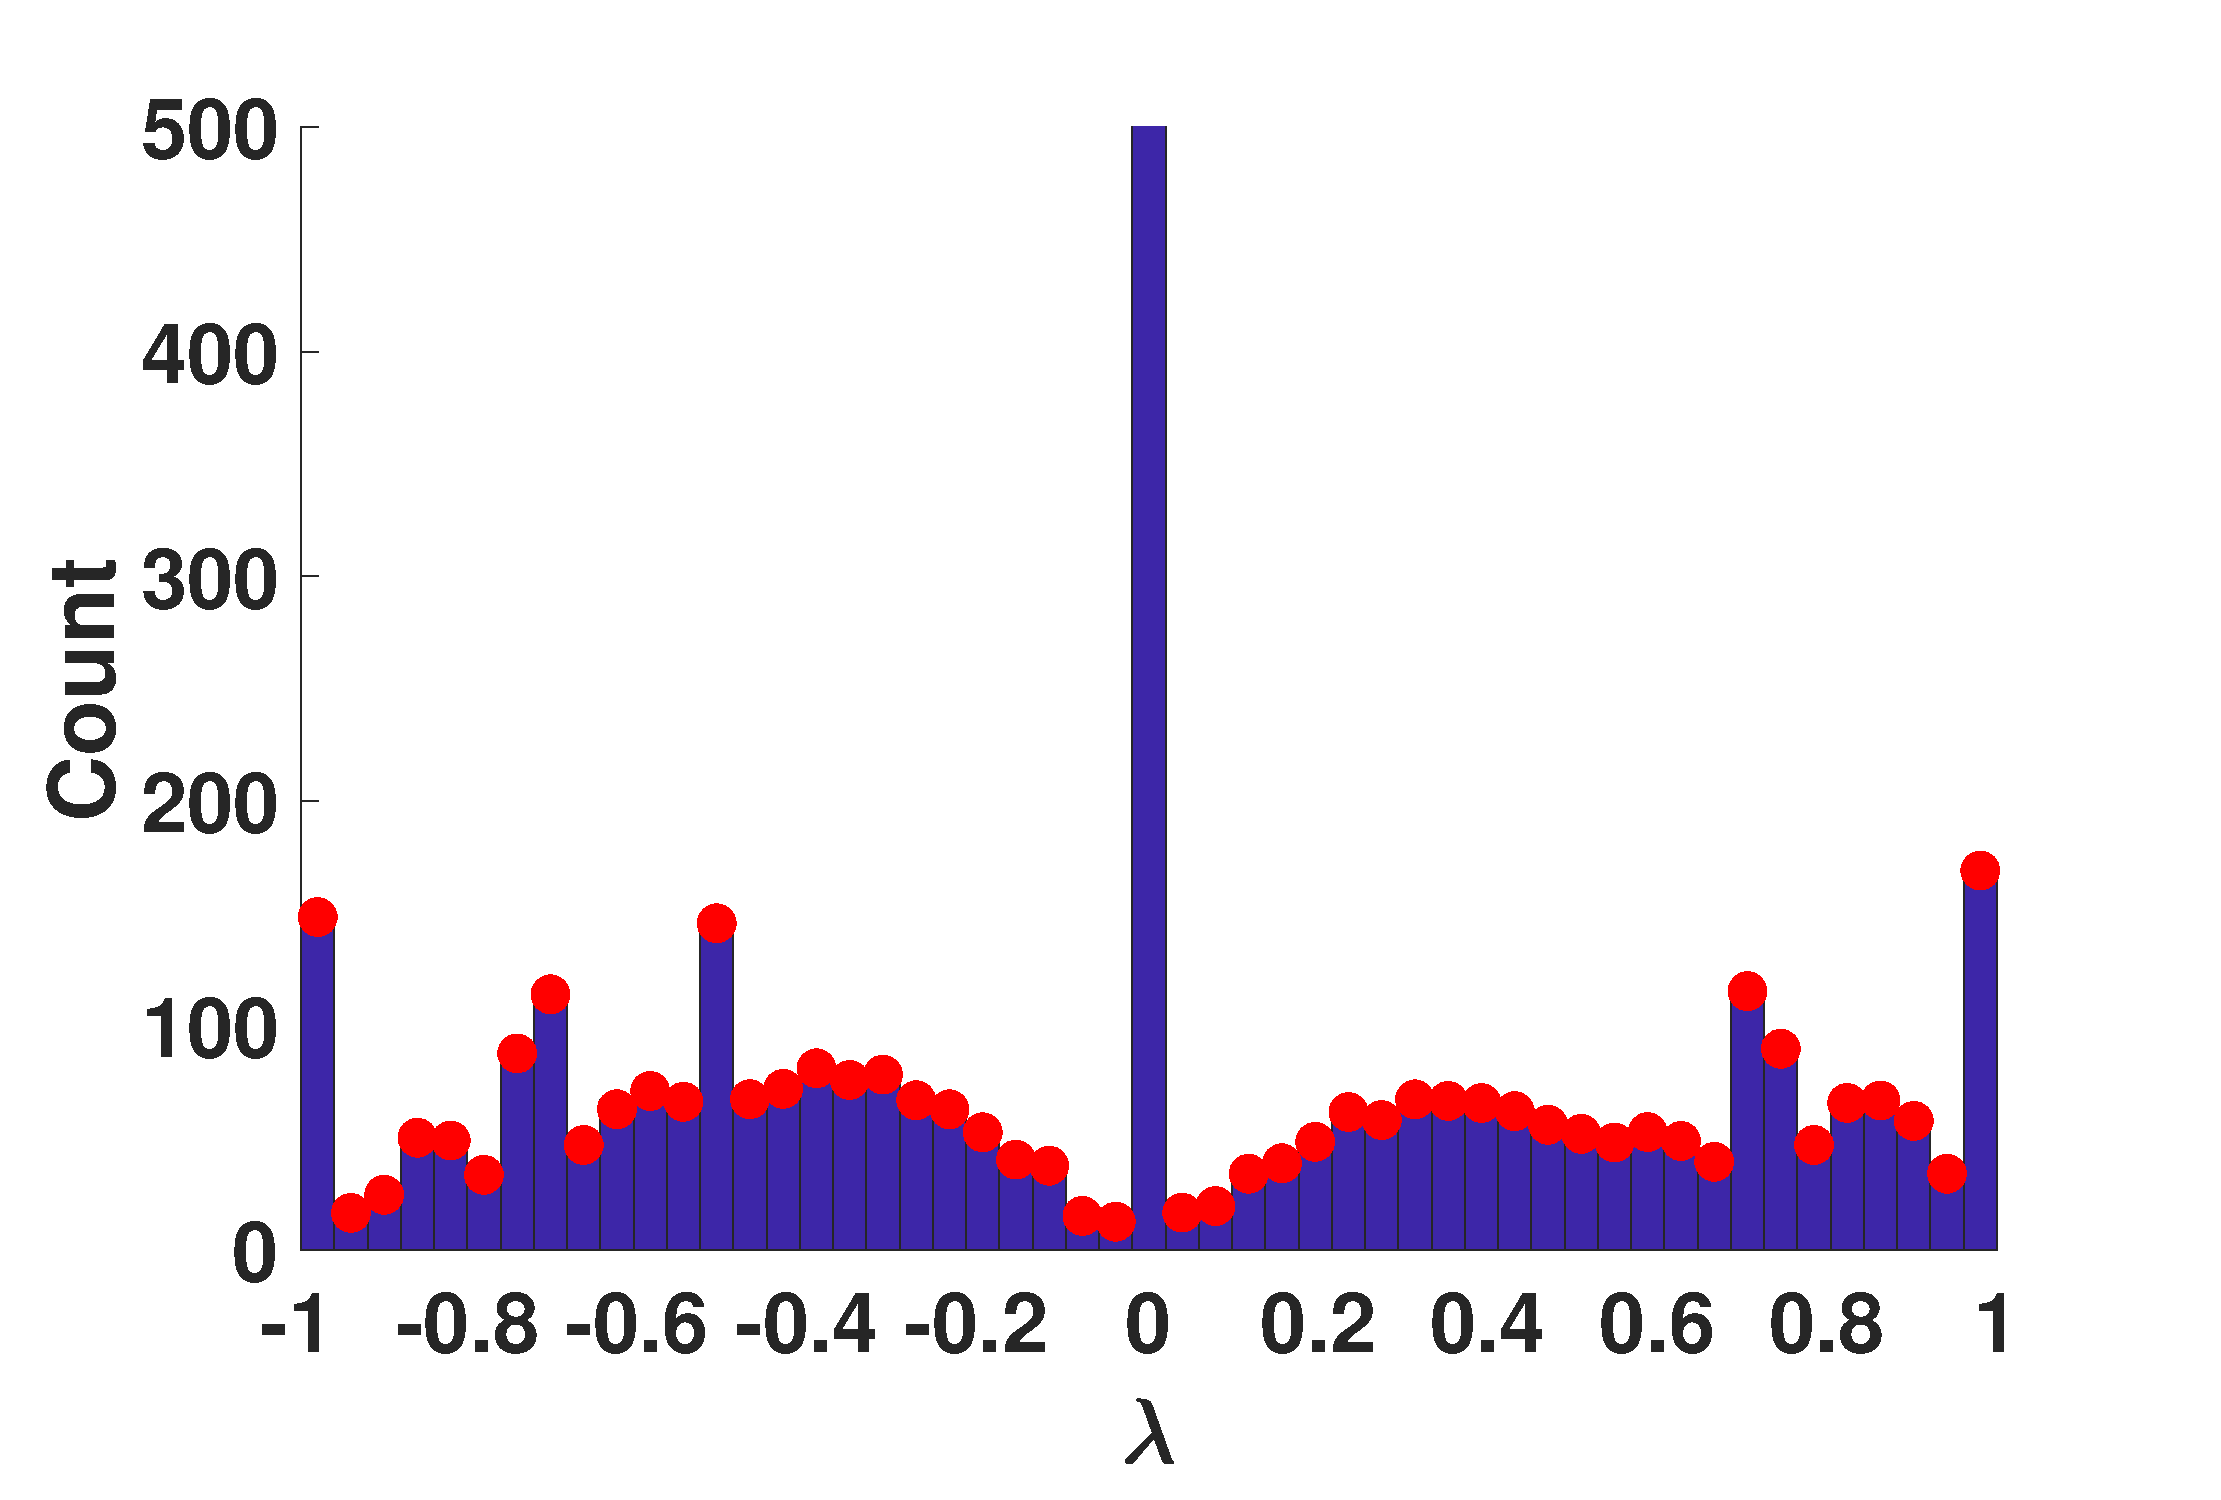
\includegraphics[width=\textwidth,trim = .4cm 0.5cm 3.5cm 1.3cm,clip]
    {./ndos/pics/bter_dos}
    \caption{BTER DOS}
    \label{fig:bter_dos}
  \end{subfigure}
  %
  \begin{subfigure}[t]{0.47\textwidth}
    \centering
    \captionsetup{justification=centering}
    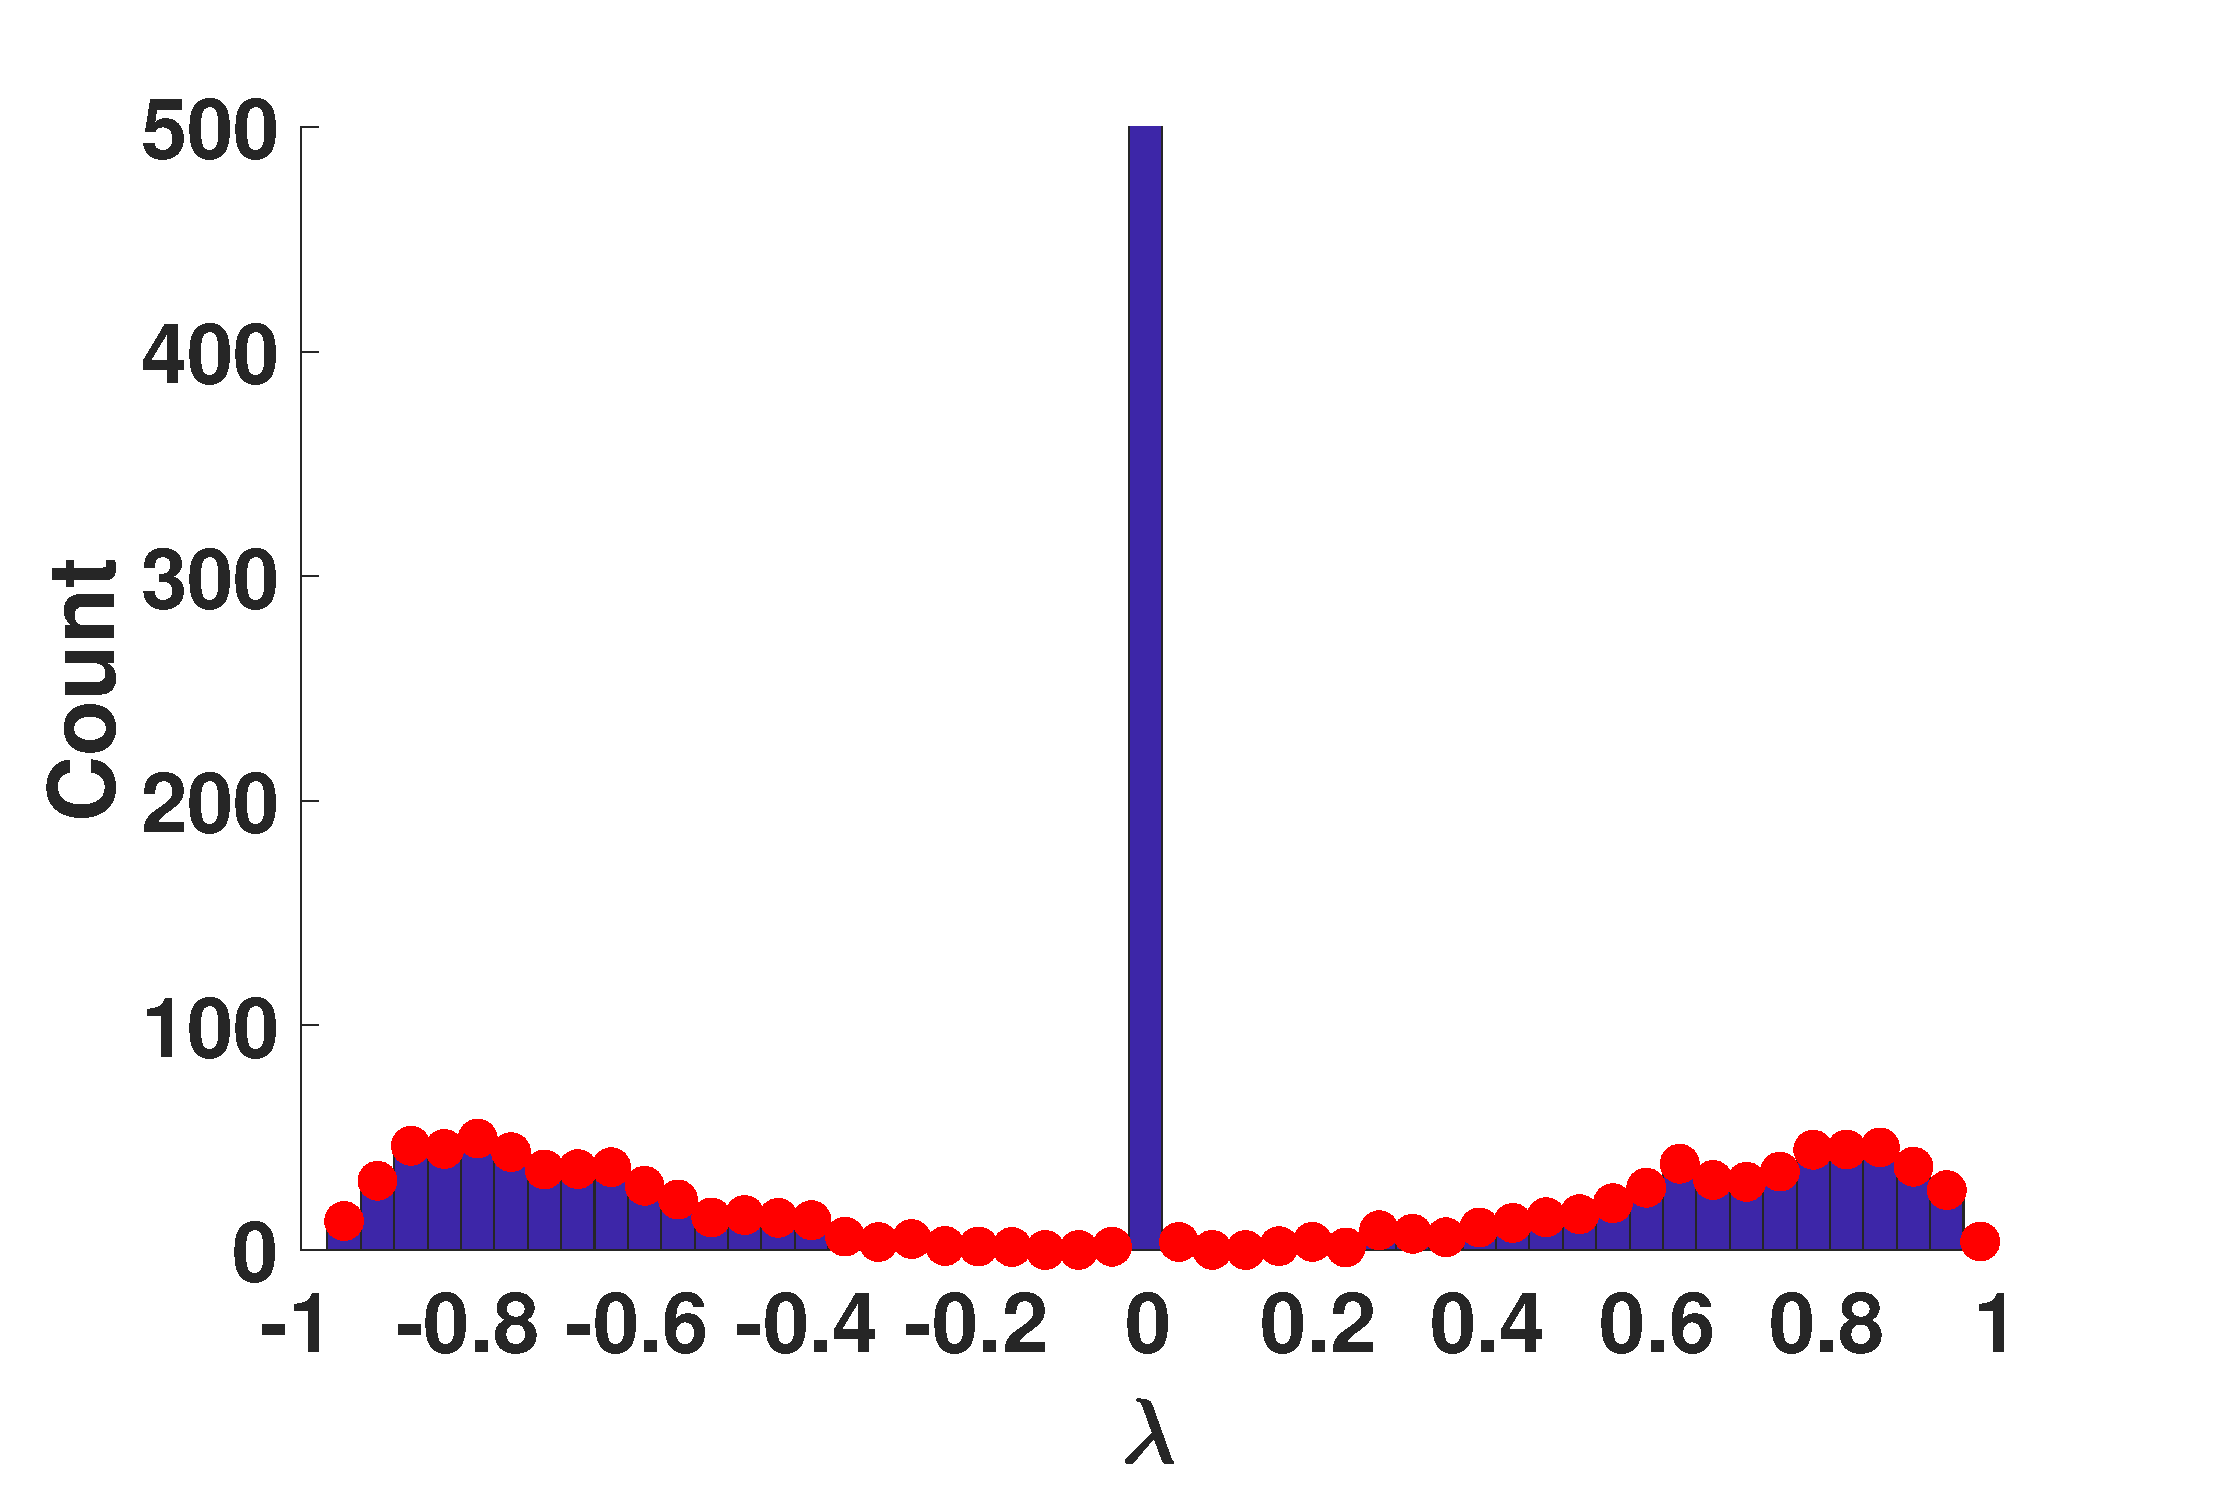
\includegraphics[width=\textwidth,trim = .4cm 0.5cm 3.5cm 1.3cm,clip]
    {./ndos/pics/erdos}
    \caption{\Erdos\ DOS}
    \label{fig:erdos_dos2}
  \end{subfigure}
  %
  \begin{subfigure}[t]{0.47\textwidth}
    \centering  
    \captionsetup{justification=centering}
    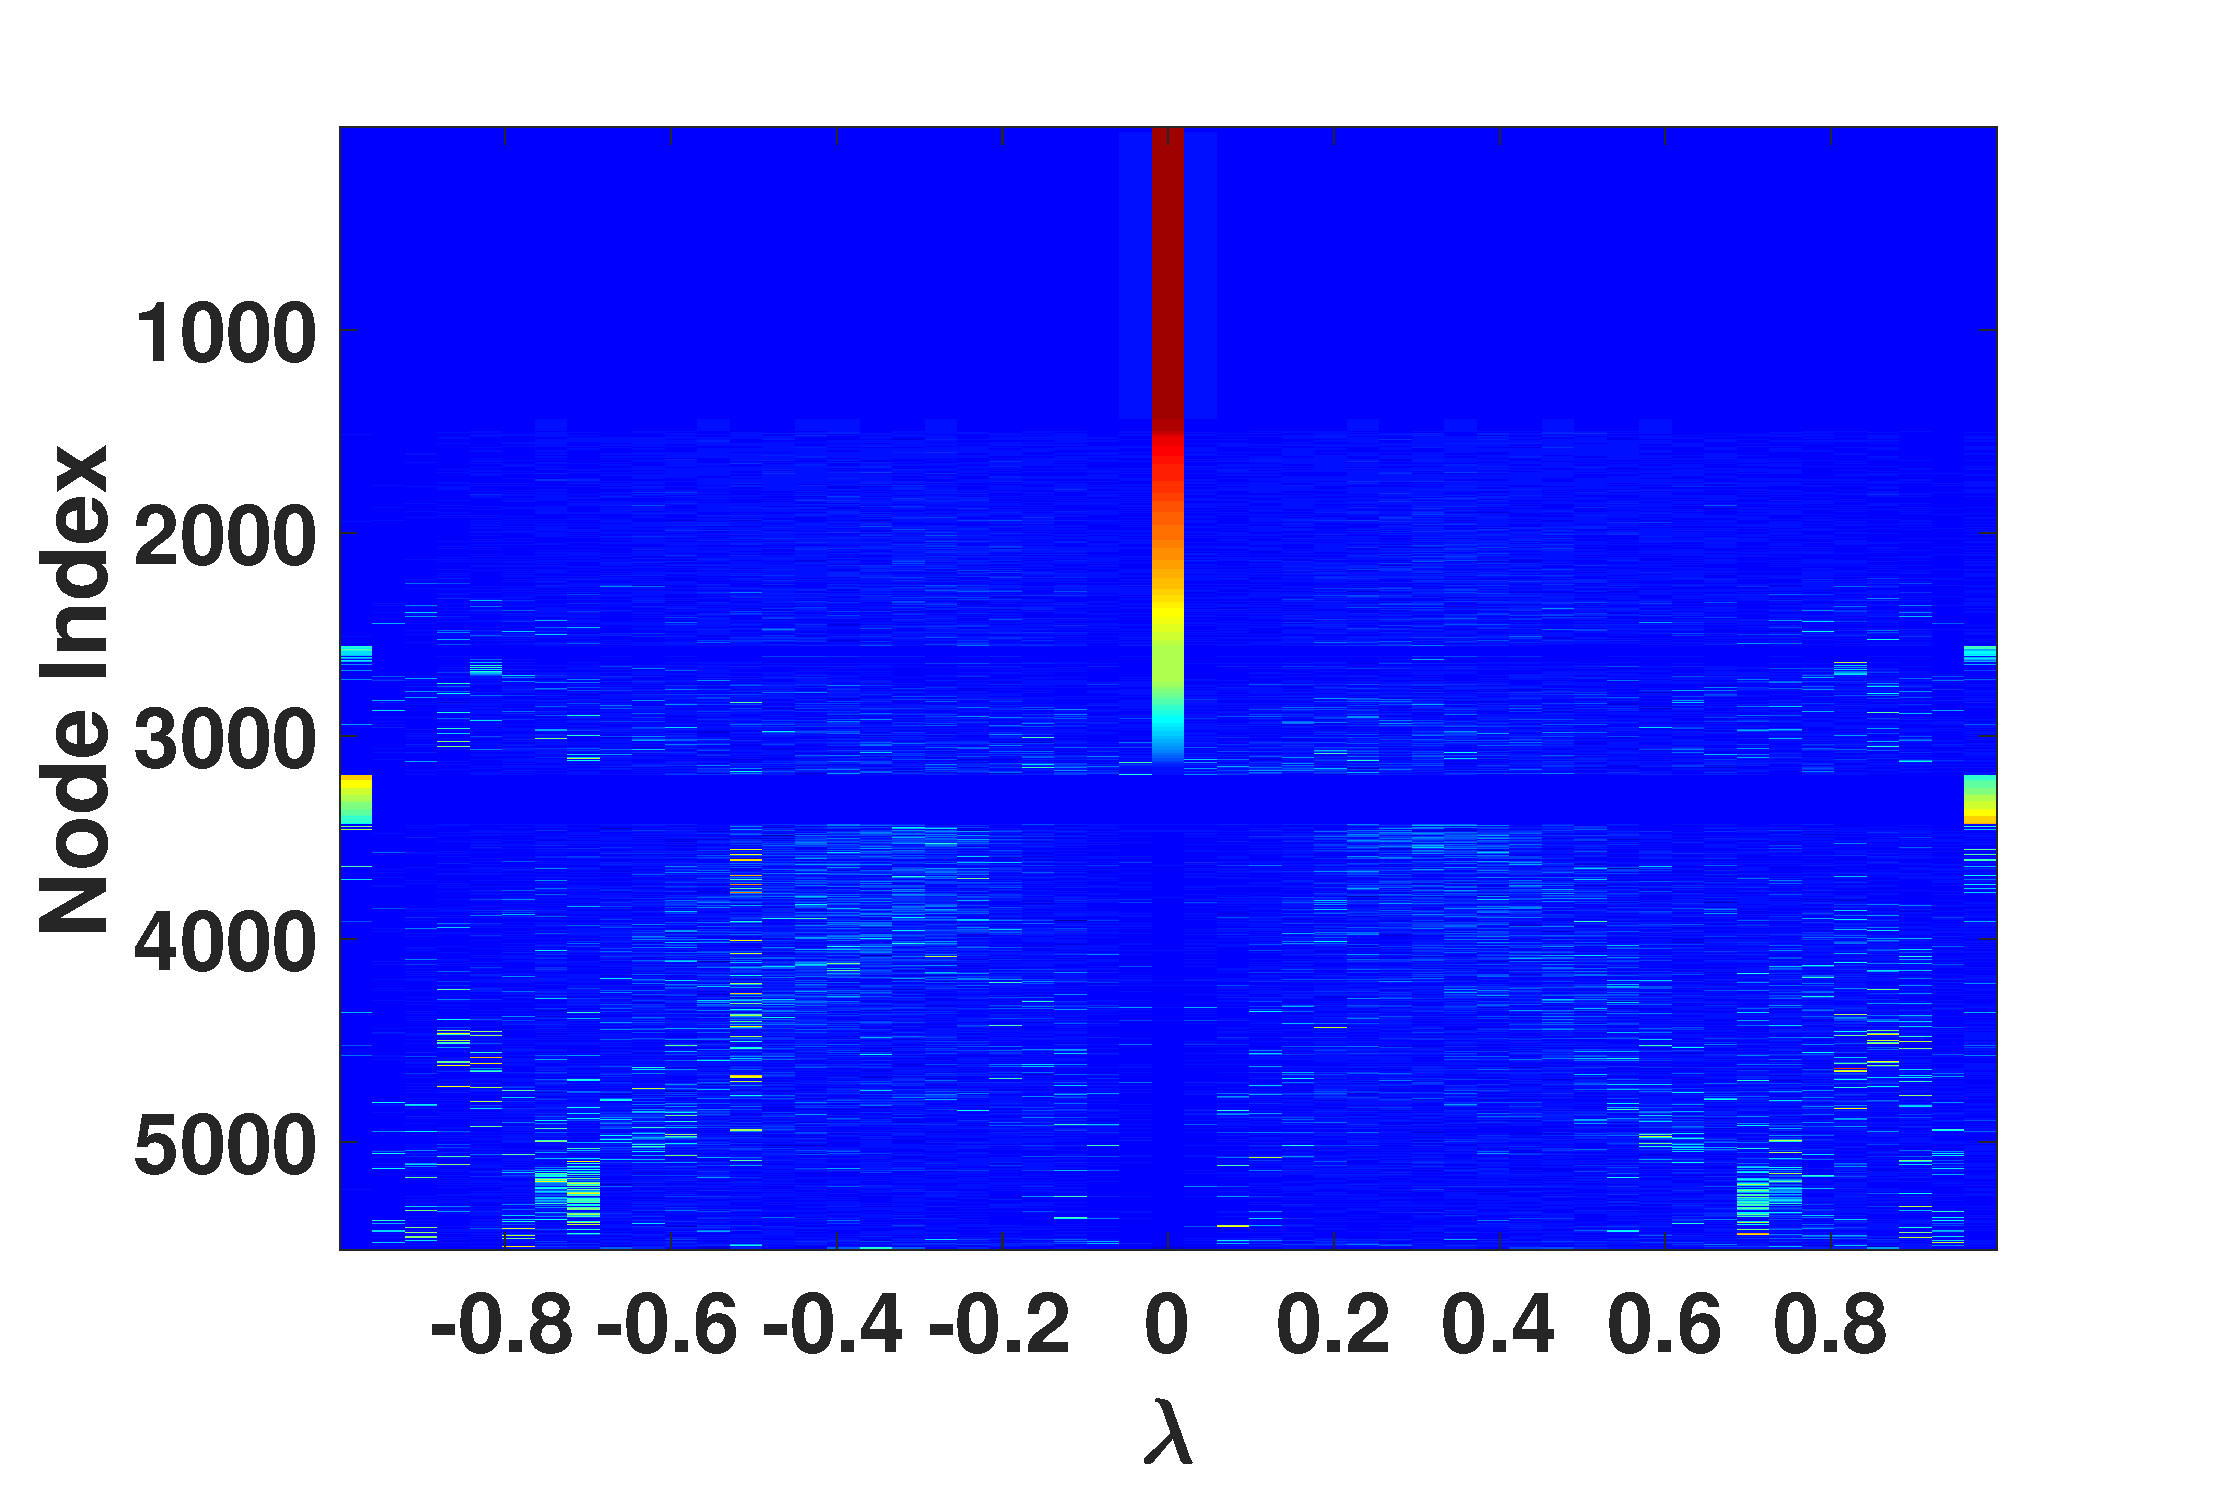
\includegraphics[width=\textwidth,trim = .4cm 0.5cm 3.5cm 1.3cm,clip]
    {./ndos/pics/bter_ldos}
    \caption{BTER PDOS}
    \label{fig:bter_ldos}
  \end{subfigure}
  \hspace{1cm}
  \begin{subfigure}[t]{0.47\textwidth}
    \centering
    \captionsetup{justification=centering}
    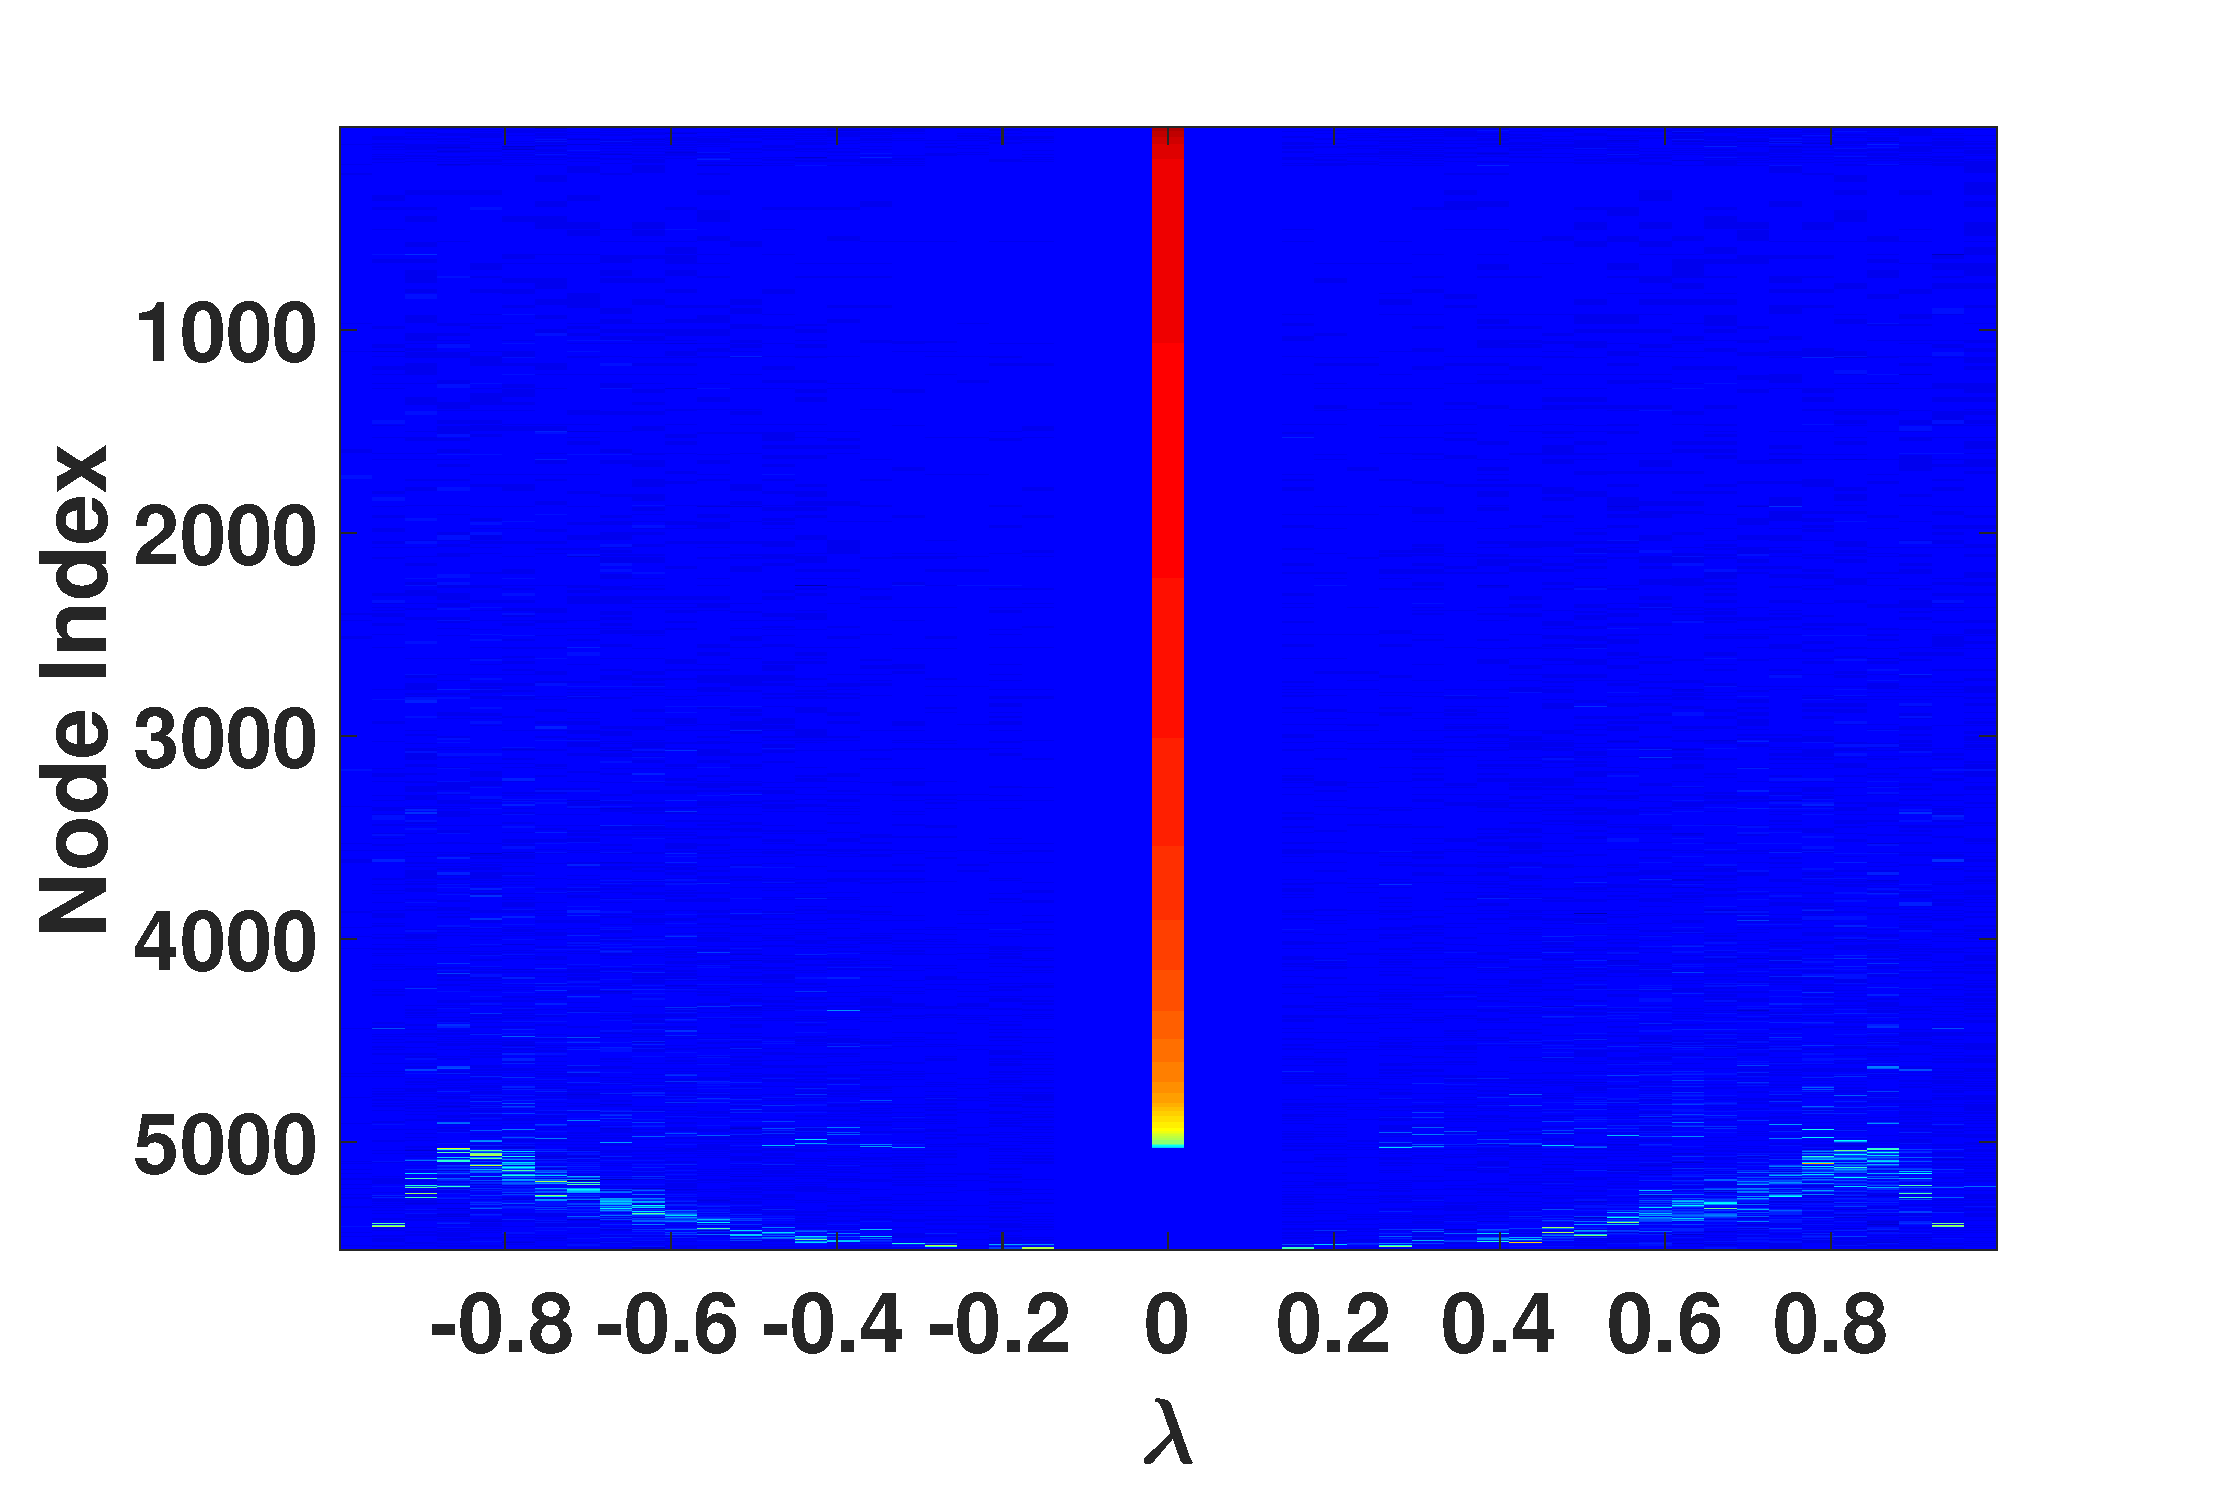
\includegraphics[width=\textwidth,trim = .4cm 0.5cm 3.5cm 1.3cm,clip]
    {./ndos/pics/erdos_ldos}
    \caption{\Erdos\ PDOS}
    \label{fig:erdos_ldos2}
  \end{subfigure}
  \caption{Comparison of spectral histogram between \Erdos\ Collaboration
  Network and the BTER model. Both DOS and PDOS are computed with $500$ moments
  and $20$ probe vectors.} \label{fig:bter}
\end{figure}

\section{Conclusion}\label{ndossec:con}
	In this paper, we make the computation of spectral densities a practical tool
for the analysis of large real-world network. Our approach borrows from methods
in solid state physics, but with adaptations that improve performance in the
network analysis setting by special handling of graph motifs that leave
distinctive spectral fingerprints. We show that the spectral densities are
stable to small changes in the graph, as well as providing an analysis of the
approximation error in our methods. We illustrate the efficiency of our
approach by treating graphs with tens of millions of nodes and billions of edges
using only a single compute node. The method provides a compelling visual
fingerprint of a graph, and we show how this fingerprint can be used for tasks
such as model verification.

Our approach opens the door for the use of complete spectral information in
large-scale network analysis. It provides a framework for scalable computation
of quantities already used in network science, such as common centrality
measures and graph connectivity indices (such as the Estrada index) that can be
expressed in terms of the diagonals and traces of matrix functions. But we
expect it to serve more generally to define new families of features that
describe graphs and the roles nodes play within those graphs. We have shown that
graphs from different backgrounds demonstrate distinct spectral
characteristics, and thus can be clustered based on those. Looking at LDOS
across nodes for role discovery, we can identify the ones with high similarity
in their local structures. Moreover, extracting nodes with large weights at
various points of the spectrum uncovers motifs and symmetries. In the future, we
expect to use DOS/LDOS as graph features for applications in graph clustering,
graph matching, role classification, and other tasks.

\noindent\textbf{Acknowledgments.} We thank NSF DMS-1620038 for supporting this
work.

\chapter{Scalable Gaussian Processes}
	\label{ch4}
	\chapnom{
\item [{$D$}]\begingroup Diagonal correction\nomeqref {4.18}\nompageref{55}
\item [{$H$}]\begingroup Preconditioner\nomeqref {4.35}\nompageref{62}
\item [{$K$}]\begingroup Kernel matrix\nomeqref {4.0}\nompageref{47}
\item [{$K^\nabla$}]\begingroup Kernel matrix with derivative information
\nomeqref {4.5}\nompageref{49}
\item [{$M$}]\begingroup Number of inducing points\nomeqref {4.0}\nompageref{46}
\item [{$N$}]\begingroup Number of data points\nomeqref {4.0}\nompageref{43}
\item [{$P$}]\begingroup Projection matrix\nomeqref {4.35}\nompageref{63}
\item [{$U$}]\begingroup Interpolation points\nomeqref {4.6}\nompageref{50}
\item [{$W$}]\begingroup Interpolation weight matrix\nomeqref {4.7}
\nompageref{51}
\item [{$\Ktil{}$}]\begingroup Kernel matrix with noise\nomeqref {4.4}
\nompageref{49}
\item [{$\calL$}]\begingroup Log marginal likelihood\nomeqref {4.4}
\nompageref{49}
\item [{$\ell$}]\begingroup Length scale\nomeqref {4.0}\nompageref{47}
\item [{$\mu$}]\begingroup Mean function\nomeqref {4.0}\nompageref{47}
\item [{$\mu^\nabla$}]\begingroup Mean function with derivative information
\nomeqref {4.5}\nompageref{49}
\item [{$\sigma$}]\begingroup Noise variance\nomeqref {4.4}\nompageref{49}
\item [{$\theta$}]\begingroup Hyper-parameters\nomeqref {4.4}\nompageref{49}
\item [{$c_j$}]\begingroup Chebyshev moments\nomeqref {4.11}\nompageref{52}
\item [{$d$}]\begingroup Dimension of data points\nomeqref {4.0}\nompageref{43}
\item [{$f$}]\begingroup Object function\nomeqref {4.0}\nompageref{47}
\item [{$k$}]\begingroup Covariance function\nomeqref {4.0}\nompageref{47}
\item [{$k^\nabla$}]\begingroup Covariance function with derivative information
\nomeqref {4.5}\nompageref{49}
\item [{$s_f$}]\begingroup Signal variance\nomeqref {4.0}\nompageref{47}
\item [{$v$}]\begingroup Predictive variance\nomeqref {4.36}\nompageref{85}
\item [{$x$}]\begingroup Data points\nomeqref {4.0}\nompageref{47}
\item [{$y$}]\begingroup Observed function value\nomeqref {4.4}\nompageref{49}
\item [{$z$}]\begingroup Probe vector\nomeqref {4.8}\nompageref{52}
}
\normalspacing

For applications as varied as Bayesian neural networks, determinantal point
processes, elliptical graphical models, and kernel learning for Gaussian
processes, one must compute a log determinant of an $N \times N$ positive
definite matrix, and its derivatives -- leading to prohibitive $\calO(N^3)$
computations. We propose novel $\calO(N)$ approaches to estimating these
quantities from only fast matrix\hyp{}vector multiplications. These stochastic
approximations are based on Chebyshev, Lanczos, and surrogate models, and
converge quickly even for kernel matrices that have challenging spectra. We
leverage these approximations to develop a scalable Gaussian process approach to
kernel learning. We find that Lanczos is generally superior to Chebyshev for
kernel learning, and that a surrogate approach can be highly efficient and
accurate with popular kernels.

On the other hand, gradient information greatly enhances the performance of
Gaussian processes in many applications, e.g., Bayesian optimization, implicit
surface reconstruction, and terrain reconstruction. Fitting a Gaussian processes
to function values and derivatives at $N$ points in $d$ dimensions requires
linear solves and log determinants with an ${N(d+1)\times N(d+1)}$ positive
definite matrix. Hence, the complexity for direct methods is $\calO(N^3d^3)$,
scaling not only with the number of data points but also the number of
dimensions. We adapt our methods with fast $\calO(Nd)$ matrix\hyp{}vector
multiplications, together with pivoted Cholesky preconditioning that cuts the
iterations to convergence by several orders of magnitude, allowing for fast
kernel learning and prediction. Our approaches, together  with dimensionality
reduction, allows us to scale Bayesian optimization with derivatives to
high\hyp{}dimensional problems and large evaluation budgets.

\section{Introduction}\label{sgpsec:int}
	There is a pressing need for scalable machine learning approaches to extract
rich statistical structure from large datasets. A common bottleneck --- arising
in determinantal point processes \cite{kulesza2012determinantal}, Bayesian
neural networks \cite{mackay1992bayesian}, model comparison 
\cite{mackay2003information}, graphical models \cite{rue2005gaussian}, and
Gaussian process kernel learning \cite{rasmussen06} --- is computing a log
determinant over a large positive definite matrix. While we can approximate log
determinants by existing stochastic expansions relying on matrix\hyp{}vector
multiplications (MVMs), these approaches make assumptions, such as
near\hyp{}uniform eigenspectra \cite{boutsidis2015randomized}, which are
unsuitable in machine learning contexts. For example, the popular RBF kernel
gives rise to rapidly decaying eigenvalues. Moreover, while standard approaches,
such as stochastic power series, have reasonable asymptotic complexity in the
rank of the matrix, they require too many terms (MVMs) for the precision
necessary in machine learning applications.

Gaussian processes (GPs) provide a principled probabilistic kernel learning
framework, for which a log determinant is of foundational importance.
Specifically, the \emph{marginal likelihood} of a Gaussian process is the
probability of data given only kernel hyper\hyp{}parameters. This utility
function for kernel learning compartmentalizes into automatically calibrated
model fit and complexity terms --- called \emph{automatic Occam's razor} ---
such that the simplest models which explain the data are automatically favored 
\cite{rasmussen01, rasmussen06}, without the need for approaches such as
cross\hyp{}validation, or regularization, which can be costly, heuristic, and
involve substantial hand\hyp{}tuning and human intervention. The automatic
complexity penalty, called the \emph{Occam's factor} 
\cite{mackay2003information}, is a log determinant of a kernel (covariance)
matrix, related to the volume of solutions that can be expressed by the Gaussian
process. Unfortunately, calculating log determinant is usually very expensive
for huge matrices. The exact kernel learning costs of $\calO (N^3)$ flops and
the prediction cost of $\calO(N)$ flops per test point are clearly
computationally infeasible for large datasets. As a result, GPs have
traditionally been limited to a few thousand data points.

In addition, derivative information greatly enhances the performance of GPs in
many applications, including Bayesian Optimization (BO) \citep{wu2017bayesian},
implicit surface reconstruction \citep{macedo2011hermite}, and terrain
reconstruction.  For many simulation models, derivatives may be computed at
little extra cost via finite differences, complex step approximation, an adjoint
method, or algorithmic differentiation \citep{forrester2008engineering}. Hence,
there are ample opportunities in learning better GP models through exploiting
derivative information in practice. However, the computation becomes more
challenging if we consider GPs with both function value and derivative
information, in which case training and prediction become $\calO(N^3d^3)$ and
$\calO(Nd)$ respectively for data points in $d$\hyp{}dimensional space
\citep[\S9.4]{rasmussen06}.

Many current approaches to scalable Gaussian processes \cite[e.g.,][]
{quinonero2005unifying,le2013fastfood,hensman2013uai} focus on inference
assuming a fixed kernel, or use approximations that do not allow for very
flexible kernel learning \cite{wilson2014thesis}, due to poor scaling with
number of basis functions or inducing points. Alternatively, approaches which
exploit algebraic structure in kernel matrices can provide highly expressive
kernel learning \cite{wilson2014fast}, but are essentially limited to grid
structured data. On the other hand, while many scalable approximation methods
for Gaussian process regression have been proposed, scalable methods
incorporating derivatives have received little attention.

Recently, \citet{wilson2015kernel} proposed the {\em structured kernel
interpolation} (SKI) framework, which generalizes structuring exploiting methods
to arbitrarily located data. SKI works by providing accurate and fast
matrix\hyp{}vector multiplies (MVMs) with kernel matrices, which can then be
used in iterative solvers such as linear conjugate gradients for scalable GP
inference. However, evaluating the marginal likelihood and its derivatives, for
kernel learning, has followed a scaled eigenvalue approach 
\citep{wilson2014fast,wilson2015kernel} instead of iterative MVM approaches.
This approach can be inaccurate, and relies on a fast eigendecomposition of a
structured matrix, which is not available in many consequential situations where
fast MVMs are available, including: (i) additive covariance functions, (ii)
multi\hyp{}task learning, (iii) change\hyp{}points \citep{herlands2016scalable},
and (iv) diagonal corrections to kernel approximations 
\citep{snelson2006sparse}. Fiedler \citep{fiedler84hankelLoewner} and Weyl 
\citep{weyl1912} bounds have been used to extend the scaled eigenvalue approach 
\citep{flaxman2015fast,herlands2016scalable}, but are similarly limited. These
extensions are often very approximate, and do not apply beyond sums of two and
three matrices, where each matrix in the sum must have a fast
eigendecomposition.

In machine learning there has recently been renewed interest in MVM based
approaches to approximating log determinants, such as the Chebyshev 
\citep{han2015large} and Lanczos\citep{ubarufast} based methods, although these
approaches go back at least two decades in quantum chemistry computations 
\citep{bai1998computing}. Independently, several authors have proposed various
methods to compute derivatives of log determinants~\citep{mackay1997efficient,
stein2013stochastic}. But {\em both} the log determinant {\em and} the
derivatives are needed for efficient GP marginal likelihood learning: the
derivatives are required for gradient\hyp{}based optimization, while the log
determinant itself is needed for model comparison, comparisons between the
likelihoods at local maximizers, and fast and effective choices of starting
points and step sizes in a gradient\hyp{}based optimization algorithm.

In this chapter, we develop novel scalable and general purpose Chebyshev,
Lanczos, and surrogate approaches for efficiently and accurately computing both
the log determinant and its derivatives simultaneously. Our methods use only
fast MVMs, and re\hyp{}use the same MVMs for both computations. We also propose
scalable methods for GPs with derivative information built on the the SKI
framework. As the uniform grids in SKI scale poorly to high\hyp{}dimensional
spaces, we further extend the structured kernel interpolation for products 
(SKIP) method, which approximates a high\hyp{}dimensional product kernel as a
Hadamard product of low rank Lanczos decompositions \citep{gardner2018product}.
Both SKI and SKIP provide fast approximate kernel MVMs, which are a building
block to solve linear systems with the kernel matrix and to approximate log
determinants~\citep{dong2017scalable}. In particular, our contributions are:
\begin{itemize}
  \item We derive fast methods for simultaneously computing the log determinant
  and its derivatives by stochastic Chebyshev, stochastic Lanczos, and surrogate
  models, from MVMs alone. We also perform an error analysis and extend these
  approaches to higher order derivatives.

  \item These methods enable fast GP kernel learning whenever fast MVMs are
  possible, including applications where alternatives such as scaled eigenvalue
  methods (which rely on fast eigendecompositions) are not, such as for (i)
  diagonal corrections for better kernel approximations, (ii) additive
  covariances, (iii) multi\hyp{}task approaches, and (iv) non\hyp{}Gaussian
  likelihoods.

  \item We extend SKI to incorporate derivative information, enabling $\calO
  (Nd)$ complexity learning and $\calO(1)$ prediction per test points, relying
  only on fast MVM with the kernel matrix.

  \item We also extend SKIP, which enables scalable Gaussian process regression
  with derivatives in high\hyp{}dimensional spaces without grids. Our approach
  allows for $\calO(Nd)$ MVMs after the inclusion of derivative information.

  \item We illustrate that preconditioning is critical for fast convergence of
  iterations for kernel matrices with derivatives. A pivoted Cholesky
  preconditioner cuts the iterations to convergence by several orders of
  magnitude when applied to both SKI and SKIP with derivatives.

  \item For GPs without derivative information, we illustrate the performance of
  our approach on several large, multi\hyp{}dimensional datasets, including a
  consequential crime prediction problem, and a precipitation problem with $N =
  528,474$ training points. We consider a variety of kernels, including deep
  kernels \citep{wilson2016deep}, diagonal corrections, and both Gaussian and
  non\hyp{}Gaussian likelihoods.

  \item For GPs with derivative information, we illustrate the scalability of
  our approach on several examples including implicit surface fitting of the
  Stanford bunny, rough terrain reconstruction, and Bayesian optimization. We
  show how our methods, together with active subspace techniques, can be used to
  extend Bayesian optimization to high\hyp{}dimensional problems with large
  evaluation budgets.

  \item We have released code and tutorials as an extension to the GPML library 
  \citep{rasmussen10gpml} at \url{https://github.com/kd383/GPML_SLD}. A Python
  implementation of our approach is also available through the GPyTorch library:
  \url{https://github.com/jrg365/gpytorch}. The code for GPs with derivative
  information is available at 
  \url{https://github.com/ericlee0803/GP_Derivatives}.
\end{itemize}

When using our approach in conjunction with SKI \citep{wilson2015kernel} for
fast MVMs, derivative\hyp{}free GP kernel learning is $\mathcal{O}(N + g(M))$,
for $M$ inducing points and $N$ training points, where $g(M) \leq M \log M$.
With algebraic approaches such as SKI we also do not need to worry about
quadratic storage in inducing points, since symmetric Toeplitz and Kronecker
matrices can be stored with at most linear cost, without needing to explicitly
construct a matrix.

Although we here use SKI for fast MVMs, we emphasize that the proposed iterative
approaches are generally applicable, and can easily be used in conjunction with
\emph{any} method that admits fast MVMs, including classical inducing point
methods \citep{quinonero2005unifying}, finite basis expansions 
\citep{le2013fastfood}, and the popular stochastic variational approaches 
\citep{hensman2013uai}. Moreover, stochastic variational approaches can
naturally be combined with SKI to further accelerate MVMs 
\citep{wilson2016stochastic}.

We start in \cref{sgpsec:bac} with an introduction to GPs and kernel
approximations.  In \cref{sgpsec:met} we introduce stochastic trace
estimation, Chebyshev (\cref{sgpsec:che}) and Lanczos (\cref{sgpsec:lan})
approximations, and various techniques we use to efficiently evaluate log
determinant for kernel matrices. In \cref{sgpsec:err}, we describe the
different sources of error in our approximations. In \cref{sgpsec:dmet}, we
extend the methods in \cref{sgpsec:met} for GPs with derivative information. In
\cref{sgpsec:exp} we consider experiments for derivative\hyp{}free GPs on
several large real\hyp{}world data sets. In \cref{sgpsec:dexp}, we demonstrate
the benefit of including derivative information, as well as the performance of
our methods in this case. We conclude in \cref{sgpsec:con}.

\section{Background}\label{sgpsec:bac}
	A Gaussian process (GP) is a collection of random variables, any finite number
of which have a joint Gaussian distribution \citep[e.g.,][]{rasmussen06}. A GP
can be used to define a distribution over functions $f(x) \sim \GP(\,\mu
(x)\,,\,k(x, x'))$, where each function value is a random variable indexed by $x
\in \BBR^d$, and $\mu\Colon \BBR^d \mathbin{\rightarrow} \BBR$ and $k\Colon
\BBR^d \times\BBR^d\mathbin{\rightarrow} \BBR$ are the mean and covariance
functions of the process.

Two popular covariance kernels are the RBF kernel
\begin{equation}\label{eqn:kernel_rbf}
  k_{\text{RBF}}(x, x') = s_f^2 \exp\left(\frac{\norm{x-x'}^2}{2\ell^2}\right)
\end{equation}
and the Mat\'ern kernel
\begin{equation}\label{eqn:kernel_matern}
  k_{\text{Mat},{\nu}}(x,x') =  s_f^2\frac{2^{1-\nu}}{\Gamma(\nu)} \left(
  \sqrt{2\nu}\frac{\norm{x-x'}}{\ell}\right)^\nu K_\nu\left(\sqrt{2\nu}
  \frac{\norm{x-x'}}{\ell}\right)
\end{equation}
where $1/2$, $3/2$, and $5/2$ are popular choices for $\nu$ to model 
heavy\hyp{}tailed correlations between function values. The spectral behavior of
these and other kernels has been well\hyp{}studied for years, and we recommend
\citep{wathen2015spectral} for recent results. Particularly relevant to our
discussion is a theorem due to Weyl, which says that if a symmetric kernel has
$\nu$ continuous derivatives, then the eigenvalues of the associated integral
operator decay like $\abs{\lambda_n} = \calo(n^{-\nu-1/2})$.  Hence, the
eigenvalues of kernel matrices for the smooth RBF kernel (and of any given
covariance matrix based on that kernel) tend to decay much more rapidly than
those of the less smooth Mat\'ern kernel, which has two derivatives at zero for
$\nu = 5/2$, one derivative at zero for $\nu = 3/2$, and no derivatives at zero
for $\nu = 1/2$.  This matters to the relative performance of Chebyshev and
Lanczos approximations of the log determinant for large values of $s_f$ and
small values of $\sigma$ on the exact and approximate RBF kernel. We also
introduce the spline kernel that we used in one of the experiments.
\begin{align}
  k_{\text{spline}}(x, y) = 
  \begin{cases}
    s^2 \big( \| x - y \|^3 + a\| x - y \|^2 + b \big) & d \text{ odd} \\
    s^2 \big( \| x - y \|^2\,\log \| x - y \| + a\| x - y \|^2 + b \big)  & d \text{ even}
  \end{cases}
\end{align}
where $a,b$ are chosen to make the spline kernel symmetric and positive definite
on the given domain. We denote any kernel hyper\hyp{}parameters by the vector
$\theta$. To be concise, we try to avoid explicitly denote the dependence of $k$
and associated matrices on $\theta$.

For any locations $X = \{x_1,\ldots,x_N\} \subset \BBR^d$, $f_X \Sim \calN
(\mu_X, \K{XX})$ where $f_X$ and $\mu_X$ represent the vectors of function
values for $f$ and $\mu$ evaluated at each of the $x_i \In X$, and $\K{XX}$ is
the matrix whose $(i,j)$ entry is $k(x_i, x_j)$. Suppose we have a vector of
corresponding function values $y \In \BBR^N$, where each entry is contaminated
by independent Gaussian noise with variance $\sigma^2$. Under a Gaussian process
prior depending on the covariance hyper\hyp{}parameters $\theta$, the log
marginal likelihood is given by
\begin{equation}\label{eqn:mloglik}
  \calL(\theta|y) = -\frac{1}{2}\left[(y-\mu_X)^T\alpha + \log\abs{\Ktil{XX}}
  + N\log 2\pi\right]\,,
\end{equation}
where $\alpha = \Ktil{XX}^{-1}(y-\mu_X)$ and $\Ktil{XX} = \K{XX} +\sigma^2I$.
Optimization of (\ref{eqn:mloglik}) is expensive, since the cheapest way of
evaluating $\log\abs{\Ktil{XX}}$ and its derivatives without taking advantage
of the structure of $\Ktil{XX}$ involves computing the $\calO(N^3)$ Cholesky
factorization of $\Ktil{XX}$. $\calO(N^3)$ computations is too expensive for
inference and learning beyond even just a few thousand points.

Meanwhile, differentiation is a linear operator, and (assuming a 
twice\hyp{}differentiable kernel) we may define a multi\hyp{}output GP for the
function and (scaled) gradient values with mean and kernel functions
\begin{equation}\label{eqn:meankernelderiv}
  \mu^{\nabla}(x) =
  \begin{bmatrix}
    \mu(x) \\ \dx_x \mu(x)
  \end{bmatrix}\,, \qquad
  k^{\nabla}(x,x') =
  \begin{bmatrix}
    k(x,x') & \left( \dx_{x'} k(x,x') \right)^T \\
    \dx_x k(x,x') & \ddx k(x,x')
  \end{bmatrix}\,,
\end{equation}
where $\dx_x k(x,x')$ and $\ddx k(x,x')$ represent the column vector of 
(scaled) partial derivatives in $x$ and the matrix of (scaled) second partials
in $x$ and $x'$, respectively. Scaling derivatives by a natural length scale
gives the multi\hyp{}output GP consistent units, and lets us understand
approximation error without weighted norms. As in the scalar GP case, we model
measurements of the function as contaminated by independent Gaussian noise.

Because the kernel matrix for the GP on function values alone is a submatrix
of the kernel matrix for function values and derivatives together, the
predictive variance in the presence of derivative information will be strictly
less than the predictive variance without derivatives. Hence, convergence of
regression with derivatives is always superior to convergence of regression
without, which is well\hyp{}studied in,~e.g.~\cite[Chapter 7]{rasmussen06}. 
\cref{fig:branin} illustrates the value of derivative information; fitting with
derivatives is evidently much more accurate than fitting function values alone.
In higher-dimensional problems, derivative information is even more valuable,
but it comes at a cost: the kernel matrix $K^{\nabla}_{XX}$ is of size $N
(d+1)$\hyp{}by\hyp{}$N(d+1)$. Scalable approximate solvers are therefore vital
in order to use GPs for large datasets with derivative data, particularly in
high\hyp{}dimensional spaces.

\begin{figure}[ht]
  \begin{center}
    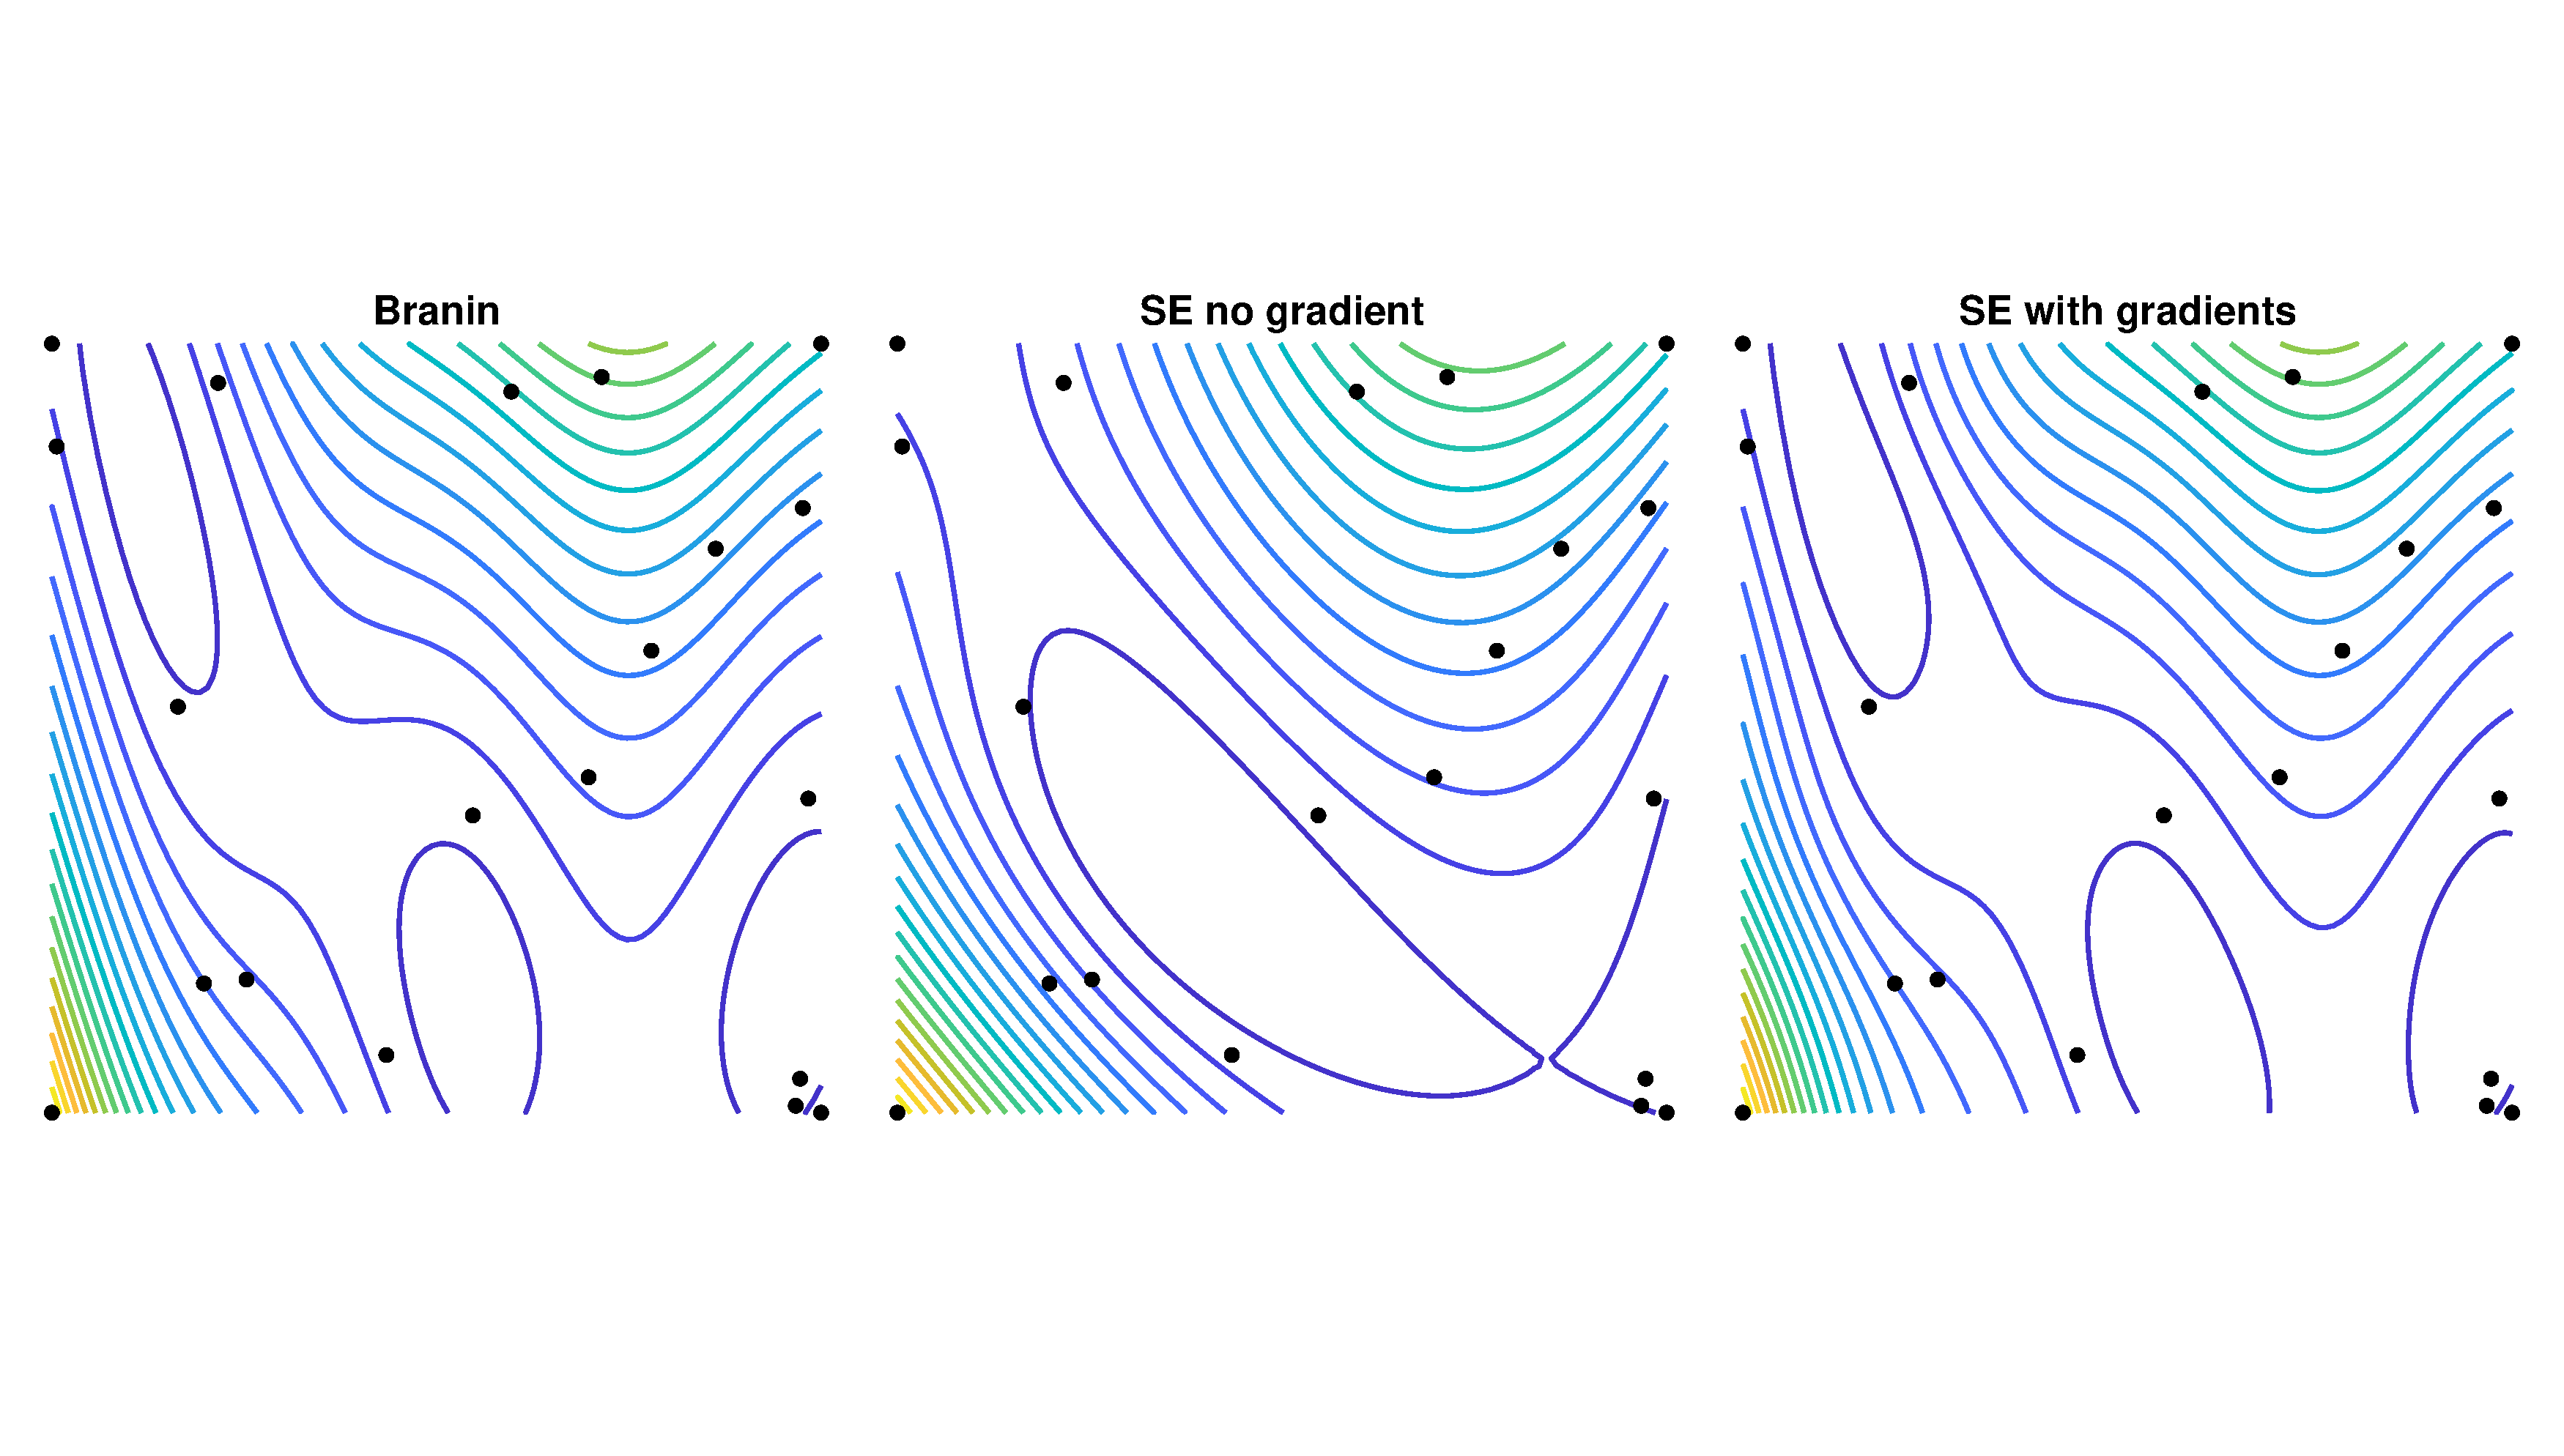
\includegraphics[width=\textwidth]{./sgpd/pics/branin}
    \caption{An example where gradient information pays off; the true function
    is on the left. Compare the regular GP without derivatives (middle) to the
    GP with derivatives (right). Unlike the former, the latter is able to
    accurately capture critical points of the function.}\label{fig:branin}
  \end{center}
\end{figure}

A popular approach to GP scalability is to replace the exact kernel $k(x, z)$
by an approximate kernel that admits fast computations 
\cite{quinonero2005unifying}. Several methods approximate $k(x, z)$ via {\em
inducing points} $U = \{u_j\}_{j=1}^M \binsubset \BBR^d$. An example is the
subset of regressor (SoR) kernel:
\begin{equation}\label{eqn:SoR}
  k^{\SoR}(x, z) = \K{xU}\K{UU}^{-1}\K{Uz}\,,
\end{equation}
which is a low\hyp{}rank approximation \cite{silverman1985some}. The SoR matrix
$\Ktil{XX}^{\SoR} \In \BBR^{N \times N}$ has rank at most $M$, allowing us to
solve linear systems involving $\Ktil{XX}^{\SoR} = \K{XX}^{\SoR} + \sigma^2I$
and to compute $\log\abs{\Ktil{XX}^{\SoR}}$ in $\calO(M^2 N + M^3)$ time.
Another popular kernel approximation is the fully independent training
conditional (FITC), which is a diagonal correction of SoR so that the diagonal
is the same as for the original kernel \cite{snelson2006sparse}.  Thus kernel
matrices from FITC have low\hyp{}rank plus diagonal structure. This modification
has had exceptional practical significance, leading to improved point
predictions and much more realistic predictive uncertainty 
\cite{quinonero2005unifying,quinonero2007}, making FITC arguably the most
popular approach for scalable Gaussian processes.

\citet{wilson2015kernel} provides a mechanism for fast MVMs through proposing
the structured kernel interpolation (SKI) approximation,
\begin{equation}\label{eqn:ski}
  \K{XX} \approx W \K{UU} W^{T}\,,
\end{equation}
where $W$ is an $N$\hyp{}by\hyp{}$M$ matrix of interpolation weights; the
authors of~\cite{wilson2015kernel} use local cubic interpolation so that $W$ is
sparse. The sparsity in $W$ makes it possible to naturally exploit algebraic
structure (such as Kronecker or Toeplitz structure) in $\K{UU}$ when the
inducing points $U$ are on a grid, for extremely fast matrix vector
multiplications with the approximate $\K{XX}$ even if the data inputs $X$ are
arbitrarily located. For instance, if $\K{UU}$ is Toeplitz, then each MVM with
the approximate $\K{XX}$ costs only $\calO(N + M \log M)$. By contrast, placing
the inducing points $U$ on a grid for classical inducing point methods, such as
SoR or FITC, does not result in substantial performance gains, due to the costly
cross-covariance matrices $\K{xU}$ and $\K{Uz}$. A limitation of SKI is that the
number of grid points increases exponentially with the dimension. This
exponential scaling has been addressed by structured kernel interpolation for
products (SKIP) \citep{gardner2018product}, which decomposes the kernel matrix
for a product kernel in $d$\hyp{}dimensions as a Hadamard (elemen\hyp{}wise)
product of one\hyp{}dimensional kernel matrices.

\section{Methods: Derivative-Free GPs}\label{sgpsec:met}
	Our goal is to estimate, for a symmetric positive definite matrix $\Ktil{}$,
\begin{equation}\label{eqn:ldnd}
  \log\abs{\Ktil{}} = \tr(\log(\Ktil{})) \quad \mbox{and} \quad \frac{\partial}
  {\partial \theta_i} \left[\log\abs{\Ktil{}}\right] = \tr\left( \Ktil{}^{-1}
  \left(\frac{\partial \Ktil{}}{\partial \theta_i} \right) \right),
\end{equation}
where $\log$ is the matrix logarithm \cite{higham2008functions}. We compute the
traces involved in both the log determinant and its derivative via {\em
stochastic trace estimators}~\cite{hutchinson1990stochastic}, which approximate
the trace of a matrix using only matrix\hyp{}vector products.

The key idea is introduced in \cref{pre:ste}: for a given matrix $A$ and
a random probe vector $z$ with independent entries with mean zero and variance
one, then $\tr(A) = \BBE[z^TAz]$. In this section, we let the entries of the
probe vectors be Rademacher random variables. We also estimate the trace by the
sample mean over $N_z$ independent probe vectors. Often surprisingly few probe
vectors suffice.

To estimate $\tr(\log(\Ktil{}))$, we need to multiply $\log(\Ktil{})$ by probe
vectors. We consider two ways to estimate $\log(\Ktil{})z$: by a polynomial
approximation of $\log$ or by using the connection between the Gaussian
quadrature rule and the Lanczos method \cite{han2015large,ubarufast} 
(\cref{pre:fom}). In both cases, we show how to re-use the same probe vectors
for an inexpensive coupled estimator of the derivatives. In addition, we may use
standard radial basis function interpolation of the log determinant evaluated at
a few systematically chosen points in the hyper\hyp{}parameter space as an
inexpensive surrogate for the log determinant.

\subsection{Chebyshev Approximation}\label{sgpsec:che}

As given in \cref{eqn:cheb_3term}, Chebyshev polynomials are defined by the
recursion
\begin{equation}\label{eqn:chebrecursion}
  T_0(x) = 1, \quad T_1(x) = x, \quad T_{j+1}(x) = 2xT_j(x)-T_{j-1}(x)\; \text{
  for }\; j\geq 1\,.
\end{equation}
For $f : [-1,1] \to \BBR$ the Chebyshev interpolant of degree $m$ is
\begin{equation}\label{eqn:chebinterp}
  f(x) \approx p_m(x) := \sum_{j=0}^m c_j T_j(x)\,, \quad \mbox{where } c_j = 
  \frac{2 - \delta_{j0}}{m+1} \displaystyle\sum_{k=0}^m f(x_k)T_j(x_k)\,,
\end{equation}
and $\delta_{j0}$ is the Kronecker delta and $x_k = \cos(\pi(k+1/2)/(m+1))$
for $k=0,1,2,\ldots,m$; see~\cite{gil2007numerical}. Using the Chebyshev
interpolant of $\log(1+\alpha x)$, we approximate $\log\abs{\Ktil{}}$ by
\begin{equation}\label{eqn:sdescale}
  \log\abs{\Ktil{}} -n\log\beta = \log\abs{I+\alpha B} \approx \sum_{j=0}^m
  c_j\tr(T_j(B))\,,
\end{equation}
when $B=(\Ktil{}/\beta-1)/\alpha$ has eigenvalues $\lambda_i \in (-1,1)$.

For stochastic estimation of $\tr(T_j(B))$, we only need to compute $z^T T_j
(B)z$ for each given probe vector $z$. We compute vectors $w_j=T_j(B)z$ and
$\partial w_j/\partial \theta_i$ via the coupled recurrences
\begin{align}
  w_0 &= z\,, &
  w_1 &= Bz\,, &
  w_{j+1} &= 2Bw_j - w_{j-1} \mbox{ for } j \geq 1\,, \label{eqn:chebrec_w} \\
  \frac{\partial w_0}{\partial \theta_i} &= 0\,, &
  \frac{\partial w_1}{\partial \theta_i} &= \frac{\partial B}{\partial \theta_i}
  z\,, &
  \frac{\partial w_{j+1}}{\partial \theta_i} &=
  2\left(\frac{\partial B}{\partial \theta_i} w_j + B \frac{\partial w_j}
  {\partial \theta_i}\right) - \frac{\partial w_{j-1}}{\partial \theta_i} \mbox{
  for } j \geq 1\,.\label{eqn:chebrec_dw}
\end{align}
This gives the estimators
\begin{equation}\label{eqn:logdetexp}
  \log \abs{\tilde K} \approx \BBE\left[\sum_{j=0}^m c_j z^Tw_j\right] \quad 
  \mbox{
  and } \quad \frac{\partial}{\partial \theta_i} \log\abs{\tilde K} \approx 
  \BBE\left[\sum_{j=0}^m c_j z^T\frac{\partial w_j}{\partial \theta_i}\right]\,.
\end{equation}
Thus, each derivative of the approximation costs two extra MVMs per term.

\subsection{Gauss Quadrature and Lanczos}\label{sgpsec:lan}

We can also approximate $z^T \log(\Ktil{}) z$ via a Lanczos decomposition; see~
\cite{golub2010matrices} for discussion of a Lanczos\hyp{}based computation of
$z^T f(\Ktil{}) z$ and~\cite{ubarufast,bai1998computing} for stochastic Lanczos
estimation of log determinants.  We run $m$ steps of the Lanczos algorithm,
which computes the decomposition
\begin{equation}\label{eqn:Klanczos}
  \Ktil{} Q_m = Q_m\Gamma_m+ \beta_m q_{m+1} e_m^T\,,
\end{equation}
where $Q_m = \left[q_1, q_2, \cdots, q_m\right] \in \BBR^{n \times m}$ is a
matrix with orthonormal columns such that $q_1 = z/\norm{z}$, $\Gamma_m \in
\BBR^{m \times m}$ is tridiagonal, $\beta_m$ is the residual, and $e_m$ is the
$m$-th Cartesian unit vector.  We estimate
\begin{equation} \label{eq:gaussq}
  z^T f(\Ktil{}) z \approx e_1^T f(\norm{z}^2 \Gamma_m) e_1\,,
\end{equation}
where $e_1$ is the first column of the identity. Because the Lanczos algorithm
is numerically unstable, there exist several practical implementations to
resolve this issue \cite{cullum2002lanczos,saad1992numerical}. The
approximation~\eqref{eq:gaussq} corresponds to a Gauss quadrature rule for the
Riemann\hyp{}Stieltjes integral of the measure associated with the eigenvalue
distribution of $\Ktil{}$.  It is exact when $f$ is a polynomial of degree up
to $2m-1$.  This approximation is also exact when $\Ktil{}$ has at most $m$
distinct eigenvalues, which is particularly relevant to Gaussian process
regression, since frequently the kernel matrices only have a small
number of eigenvalues that are not close to zero.

The Lanczos decomposition also allows us to estimate derivatives of the log
determinant at minimal cost. Via the Lanczos decomposition, we have
\begin{equation}\label{eqn:lansolve}
  \hat{g} = Q_m (\Gamma_m^{-1} e_1 \norm{z}) \approx \Ktil{}^{-1}z \,.
\end{equation}
This approximation requires no additional matrix vector multiplications beyond
those used to compute the Lanczos decomposition, which we already used to
estimate $\log(\Ktil{}) z$; in exact arithmetic, this is equivalent to $m$ steps
of conjugate gradient (CG). Computing $\hat{g}$ in this way takes $\calO(mN)$
additional time; subsequently, we only need one matrix-vector multiply by
$\partial \Ktil{} / \partial \theta_i$ for each probe vector to estimate $\tr
(\Ktil{}^{-1} (\partial \Ktil{} / \partial \theta_i)) = \BBE\left[(\Ktil{}^{-1}
z)^T(\partial \Ktil{}/\partial \theta_i) z\right]$.


\subsection{Diagonal Correction to SKI}\label{sgpsec:dia}

The SKI approximation may provide a poor estimate of the diagonal entries of the
original kernel matrix for kernels with limited smoothness, such as the Mat\'ern
kernel. In general, diagonal corrections to scalable kernel approximations can
lead to great performance gains.  Indeed, the popular FITC method 
\citep{snelson2006sparse} is exactly a diagonal correction of SoR.

We thus modify the SKI approximation to add a diagonal matrix $D$,
\begin{equation}\label{eqn:skidiacor}
    \K{XX} \approx W \K{UU} W^T + D\, ,
\end{equation}
such that the diagonal of the approximated $\K{XX}$ is exact. In other words,
$D$ subtracts the diagonal of $W \K{UU} W^T$ and adds the true diagonal of $K_
{XX}$.  This modification is not possible for the scaled eigenvalue method for
approximating log determinants in \citep{wilson2015kernel}, since adding a
diagonal matrix makes it impossible to approximate the eigenvalues of $\K{XX}$
from the eigenvalues of $\K{UU}$.

However, Eq.~\ref{eqn:skidiacor} still admits fast MVMs and thus works with our
approach for estimating the log determinant and its derivatives. Computing $D$
with SKI costs only $\calO(n)$ flops since $W$ is sparse for local cubic
interpolation. We can therefore compute $(W^Te_i)^T\K{UU}(W^Te_i)$ in $\calO(1)$
flops.

\subsection{Estimating Higher Derivatives}\label{sgpsec:hod}

We have already described how to use stochastic estimators to compute the log
marginal likelihood and its first derivatives. The same approach applies to
computing higher\hyp{}order derivatives for a Newton\hyp{}like iteration, to
understand the sensitivity of the maximum likelihood parameters, or for similar
tasks. The first derivatives of the full log marginal likelihood are
\begin{equation}\label{eqn:loglikderiv}
  \frac{\partial \calL}{\partial \theta_i} = -\frac{1}{2} \left[\tr\left(\Ktil
  {}^{-1} \frac{\partial \Ktil{}}{\partial \theta_i}\right) - \alpha^T 
  \frac{\partial \Ktil{}}{\partial \theta_i} \alpha\right]\,,
\end{equation}
and the second derivatives of the two terms are
\begin{align}
  \frac{\partial^2}{\partial \theta_i \partial \theta_j} \left[ \log |\tilde K|
  \right] &= \tr\left(\Ktil{}^{-1} \frac{\partial^2 \Ktil{}} {\partial \theta_i
  \partial \theta_j} - \Ktil{}^{-1} \frac{\partial \Ktil{}}{\partial \theta_i}
  \Ktil{}^{-1} \frac{\partial \Ktil{}}{\partial \theta_j}\right)\,, \\
  \frac{\partial^2}{\partial \theta_i \partial \theta_j} \left[ (y-\mu_X)^T
  \alpha \right] &= 2\alpha^T \frac{\partial \Ktil{}}{\partial \theta_i}
  \Ktil{}^{-1}\frac{\partial \tilde K}{\partial \theta_j} \alpha - \alpha^T 
  \frac{\partial^2 \Ktil{}} {\partial \theta_i \partial \theta_j}\alpha\,.
\end{align}
Superficially, evaluating the second derivatives would appear to require several
additional solves above and beyond those used to estimate the first derivatives
of the log determinant.  In fact, we can get an unbiased estimator for the
second derivatives with no additional solves, but only fast products with the
derivatives of the kernel matrices.  Let $z$ and $w$ be independent probe
vectors, and define $g = \Ktil{}^{-1}z$ and $h = \Ktil{}^{-1}w$.  Then
\begin{align}
  \frac{\partial^2}{\partial \theta_i \partial \theta_j} \left[\log\abs{\Ktil{}}
  \right] &= \BBE \left[ g^T \frac{\partial^2 \Ktil{}} {\partial \theta_i
  \partial \theta_j} z - \left( g^T \frac{\partial \Ktil{}}{\partial \theta_i}
  w \right) \left( h^T \frac{\partial \Ktil{}}{\partial \theta_j} z \right)
  \right]\,, \\
  \frac{\partial^2}{\partial \theta_i \partial \theta_j} \left[ (y-\mu_X)^T
  \alpha \right] &= 2 \BBE \left[\left( z^T \frac{\partial \Ktil{}}{\partial
  \theta_i} \alpha \right) \left( g^T \frac{\partial \Ktil{}}{\partial \theta_j}
  \alpha \right)\right] - \alpha^T \frac{\partial^2 \Ktil{}} {\partial \theta_i
  \partial \theta_j}\alpha\,.
\end{align}
Hence, if we use the stochastic Lanczos method to compute the log determinant
and its derivatives, the additional work required to obtain a second derivative
estimate is one MVM by each second partial of the kernel for each probe vector
and for $\alpha$, one MVM of each first partial of the kernel with $\alpha$, and
a few dot products.

\subsection{Surrogate Model}\label{sgpsec:rbf}

Another way to deal with the log determinant and its derivatives is to evaluate
the log determinant term at a few systematically chosen points in the space of
hyperparameters and fit an interpolation approximation to these values.  This
is particularly useful when the kernel depends on a modest number of
hyperparameters (e.g., half a dozen), and thus the number of points we need to
precompute is relatively small. We refer to this method as a surrogate, since it
provides an inexpensive substitute for the log determinant and its derivatives.
For our surrogate approach, we use radial basis function (RBF) interpolation,
which is one of the most popular models for approximating scattered data in a
general number of dimensions \citep{buhmann2000radial,fasshauer2007meshfree,
schaback2006kernel,wendland2004scattered}.
Given distinct interpolation points $\Theta=\{\theta^i\}_{i=1}^n$, the RBF model
takes the form
\begin{equation}\label{eq:rbf}
  s_{\Theta}(\theta) = \sum_{i=1}^n \lambda_i \varphi(\norm{x - \theta^i}) + p
  (x)\,,
\end{equation}
where the kernel $\varphi\Colon\mathbb{R}_{\geq 0} \to \mathbb{R}$ is a
one\hyp{}dimensional function and $p \in \Pi_{m-1}^d$, the space of polynomials
with $d$ variables of degree no more than $m-1$. There are many possible choices
for $\varphi$, such as the cubic kernel $\varphi(r)=r^3$ that we adopt in our
experiments, and the thin-plate spline kernel $\varphi(r)=r^2\,\log(r)$. The
coefficients $\lambda_i$ are determined by imposing the interpolation conditions
$s_{\Theta}(\theta^i) = \log\abs{K(\theta^i)}$ for $i=1,\ldots,n$ and the
discrete orthogonality condition
\begin{equation}\label{eq:disc_orthg}
  \sum_{i=1}^n \lambda_i q(\theta^i) = 0, \qquad \forall q \in \Pi_{m-1}^d.
\end{equation}
For appropriate RBF kernels, this linear system is nonsingular provided that
polynomials in $\Pi_{m-1}^d$ are uniquely determined by their values on the
interpolation set.

\section{Error Properties}\label{sgpsec:err}
	\subsection{First-Order Analysis}
In addition to the usual errors from sources such as solver termination criteria
and floating point arithmetic, our approach to kernel learning involves several
additional sources of error: we approximate the true kernel with one that
enables fast MVMs, we approximate traces using stochastic estimation, and we
approximate the actions of $\log(\Ktil{})$ and $\Ktil{}^{-1}$ on probe
vectors.

We can compute first\hyp{}order estimates of the sensitivity of the log
likelihood to perturbations in the kernel using the same stochastic estimators
we use for the derivatives with respect to hyper\hyp{}parameters. For example,
if $\calL^{\Ref}$ is the likelihood for a reference kernel $\Ktil{}^{\Ref} =
\Ktil{} + E$, then
\begin{equation}
  \calL^{\Ref}(\theta|y) = \calL(\theta|y) - \frac{1}{2} \left(\BBE\left
  [g^TEz\right] - \alpha^T E \alpha \right) + \calO(\norm{E}^2)\,,
\end{equation}
and we can bound the change in likelihood at first order by $\norm{E}\left(
\norm{g}\norm{z} + \norm{\alpha}^2 \right)$. Given bounds on the norms of
$\partial E/\partial \theta_i$, we can similarly estimate changes in the
gradient of the likelihood, allowing us to bound how the marginal likelihood
hyperparameter estimates depend on kernel approximations.

If $\Ktil{} = U \Lambda U^T + \sigma^2 I$, the Hutchinson trace estimator has
known variance~\cite{Avron:2011:Randomized}
\begin{equation}
  \Var\left[z^T \log(\Ktil{}) z\right] = \sum_{i \neq j} \left[\log(\Ktil
  {})\right]_{ij}^2 \leq \sum_{i=1}^n \log(1 + \lambda_j/\sigma^2)^2\,.
\end{equation}
If the eigenvalues of the kernel matrix without noise decay rapidly enough
compared to $\sigma$, the variance will be small compared to the magnitude of
$\tr(\log \Ktil{}) = 2n\log \sigma + \sum_{i=1}^n\log(1+\lambda_j/\sigma^2)$.
Hence, we need fewer probe vectors to obtain reasonable accuracy than one would
expect from bounds that are blind to the matrix structure. In our experiments,
we typically only use 5--10 probes --- and we use the sample variance across
these probes to estimate {\em a posteriori} the stochastic component of the
error in the log likelihood computation.  If we are willing to estimate the
Hessian of the log likelihood, we can increase rates of convergence for finding
kernel hyper\hyp{}parameters.

The Chebyshev approximation scheme requires $\calO(\!\!\sqrt{\kappa}
\log(\kappa/\epsilon))$ steps to obtain an $\calO(\epsilon)$ approximation error
in computing $z^T \log(\Ktil{}) z$, where $\kappa = \lambda_{\max}/\lambda_
{\min}$ is the condition number of $\Ktil{}$~\cite{han2015large}. This behavior
is independent of the distribution of eigenvalues within the interval $[\lambda_
{\min}, \lambda_{\max}]$, and is close to optimal when eigenvalues are spread
quasi-uniformly across the interval. Nonetheless, when the condition number is
large, convergence may be quite slow.  The Lanczos approach converges at least
twice as fast as Chebyshev in general~\cite[Remark 1]{ubarufast}, and converges
much more rapidly when the eigenvalues are {\em not} uniform within the
interval, as is the case with log determinants of many kernel matrices.  Hence,
we recommend the Lanczos approach over the Chebyshev approach in general.  In
all of our experiments, the error associated with approximating $z^T \log(\Ktil
{}) z$ by Lanczos was dominated by other sources of error.

\subsection{Comparison to Reference Kernel}
\label{sup:refkernel}

Suppose more generally that $\tilde K = K + \sigma^2 I$ is an approximation to a
reference kernel matrix $\tilde K^{\Ref} = K^{\Ref} + \sigma^2 I$, and let $E =
K^{\Ref}-K$.  Let $\mathcal{L}(\theta | y)$ and $\calL^{\Ref}(\theta | y)$ be
the log likelihood functions for the two kernels; then
\begin{align}
  \calL^{\Ref}(\theta | y) &=
  \calL(\theta | y) -\frac{1}{2} \left[\tr(\tilde K^{-1} E) - \alpha^T E \alpha
  \right] + \calO(\|E\|^2) \\
  \frac{\partial}{\partial \theta_i} \calL^{\Ref}(\theta | y) &=
  \frac{\partial}{\partial \theta_i} \mathcal{L}(\theta | y) - \frac{1}{2}
  \left[\tr\left( \tilde K^{-1} \frac{\partial E}{\partial \theta_i} - \tilde K^
  {-1} \frac{\partial \tilde K}{\partial \theta_i} \tilde K^{-1} E \right) -
  \alpha^T \frac{\partial E}{\partial \theta_i}  \alpha \right] + \calO
  (\norm{E}^2).
\end{align}
If we are willing to pay the price of a few MVMs with $E$, we can use these
expressions to improve our maximum likelihood estimate. Let $z$ and $w$ be
independent probe vectors with $g = \tilde K^{-1} z$ and $\hat{g} = \tilde K^
{-1} w$. To estimate the trace in the derivative computation, we use the
standard stochastic trace estimation approach together with the observation that
$\BBE[ww^T] = I$:
\begin{equation}
 \tr\left(\tilde K^{-1} \frac{\partial E}{\partial \theta_i} - \tilde K^{-1} 
 \frac{\partial \tilde K}{\partial \theta_i} \tilde K^{-1} E \right) =
 \BBE\left[ g^T \frac{\partial E}{\partial \theta_i} z - g^T \frac{\partial K}
 {\partial \theta_i} w \hat{g}^T E z\right]
\end{equation}
This linearization may be used directly (with a stochastic estimator);
alternately, if we have an estimates for $\norm{E}$ and $\norm{\partial
E/\partial \theta_i}$, we can substitute these in order to get estimated bounds
on the magnitude of the derivatives. Coupled with a similar estimator for the
Hessian of the likelihood function, we can use this method to compute the
maximum likelihood parameters for the fast kernel, then compute a correction
$-H^{-1} \nabla_{\theta} \calL^{\Ref}$ to estimate the maximum likelihood
parameters of the reference kernel.

\section{Methods: GPs with Derivative Information}\label{sgpsec:dmet}
	One standard approach to scaling GPs substitutes the exact kernel with an
approximate kernel. When the GP fits values and gradients, one may attempt to
separately approximate the kernel and the kernel derivatives. Unfortunately,
this may lead to indefiniteness, as the resulting approximation is no longer a
valid kernel. Instead, we differentiate the approximate kernel, which preserves
positive definiteness. We do this for the SKI and SKIP kernels below, but our
general approach applies to any approximate MVM.

\subsection{D-SKI}

D\hyp{}SKI (SKI with derivatives) is the standard kernel matrix for GPs with
derivatives, but applied to the SKI kernel.  Equivalently, we differentiate the
interpolation scheme:
\begin{equation}\label{eqn:weightderiv}
  k(x,x') \approx \sum_i w_i(x)k(x_i,x')\rightarrow \nabla k(x,x') \approx
  \sum_i \nabla w_i(x) k(x_i,x')\,.
\end{equation}
One can use cubic convolutional interpolation \citep{keys1981cubic}, but higher
order methods lead to greater accuracy, and we therefore use quintic
interpolation~\cite{meijering1999image}.  The resulting D\hyp{}SKI kernel matrix
has the form
\begin{equation}\label{eqn:dski}
  \begin{bmatrix} K & (\dx K)^T \\ \dx K & \ddx K \end{bmatrix}  \approx
  \begin{bmatrix} W \\ \dx W  \end{bmatrix}  K_{UU}
  \begin{bmatrix} W \\ \dx W  \end{bmatrix} ^T =
  \begin{bmatrix} W\K{UU}W^T & W\K{UU} (\dx W)^T \\
  (\dx W) \K{UU} W^T & (\dx W) \K{UU} (\dx W)^T  \end{bmatrix}\,,
\end{equation}
where the elements of sparse matrices $W$ and  $\dx W$ are determined by $w_i
(x)$and $\nabla w_i(x)$ --- assuming quintic interpolation, $W$ and $\dx W$ will
each have $6^d$ elements per row. As with SKI, we use FFTs to obtain $
\calO(M \log M)$ MVMs with $\K{UU}$. Because $W$ and $\dx W$ have $\calO(N6^d)$
and $\calO(Nd6^d)$nonzero elements, respectively, our MVM complexity is $\calO
(Nd6^d + M \log M)$.

\subsection{D-SKIP}

Several common kernels are {\em separable}, i.e., they can be expressed as
products of one\hyp{}dimensional kernels.  Assuming a compatible approximation
scheme, this structure is inherited by the SKI approximation for the kernel
matrix without derivatives,
\begin{equation}\label{eqn:ski_sep}
  K \approx (W_1 K_1 W_1^T) \odot (W_2 K_2 W_2^T) \odot \ldots \odot (W_d K_d
  W_d^T)\,,
\end{equation}
where $A \odot B$ denotes the Hadamard product of matrices $A$ and $B$ with the
same dimensions, and $W_j$ and $K_j$ denote the SKI interpolation and inducing
point grid matrices in the $j$\hyp{}th coordinate direction. The same Hadamard
product structure applies to the kernel matrix with derivatives; for example,
for $d = 2$,
\begin{equation} \label{eqn:skip}
  \resizebox{.9\hsize}{!}{
    $K^{\nabla} \approx
    \begin{bmatrix}
        W_1 K_1 W_1^T      & W_1 K_1 \dx W_1^T     & W_1 K_1 W_1^T \\
        \dx W_1 K_1 W_1^T  & \dx W_1 K_1 \dx W_1^T & \dx W_1 K_1 W_1^T \\
        W_1 K_1 W_1^T      & W_1 K_1 \dx W_1^T     & W_1 K_1 W_1^T \\
    \end{bmatrix}
    \odot
    \begin{bmatrix}
        W_2 K_2 W_2^T      & W_2 K_2 W_2^T      & W_2 K_2 \dx W_2^T \\
        W_2 K_2 W_2^T      & W_2 K_2 W_2^T      & W_2 K_2 \dx W_2^T \\
        \dx W_2 K_2 W_2^T  & \dx W_2 K_2 W_2^T  & \dx W_2 K_2 \dx W_2^T \\
    \end{bmatrix}$
  }\,.
\end{equation}

\cref{eqn:skip} expresses $K^{\nabla}$ as a Hadamard product of one dimensional
kernel matrices. Following this approximation, we apply the SKIP reduction~
\citep{gardner2018product} and use Lanczos to further approximate 
\cref{eqn:skip} as $(Q_1 \Gamma_1 Q_1^T) \odot (Q_2 \Gamma_2 Q_2^T)$. This can
be used for fast MVMs with the kernel matrix. Applied to kernel matrices with
derivatives, we call this approach D\hyp{}SKIP.

Constructing the D\hyp{}SKIP kernel costs $\calO(d^2(N + M \log M+ r^3 N \log
d))$, and each MVM costs $\calO(d r^2 N)$ flops where $r$ is the effective rank
of the kernel at each step (rank of the Lanczos decomposition). We achieve high
accuracy with $r \ll N$. 

\subsection{Preconditioning}

Recent work \citep{cutajar2016preconditioning} has explored several 
preconditioners for exact kernel matrices. We have had success with
preconditioners of the form $H = \sigma^2 I + FF^T$ where $K^\nabla \approx
FF^T$ with $F \in \BBR^{N \times r}$. Solving with the
Sherman\hyp{}Morrison\hyp{}Woodbury formula ({\em a.k.a} the matrix inversion
lemma) is inaccurate for small $\sigma$; we use the more stable formula $H^{-1}
b = \sigma^{-2} (f-Q_1 (Q_1^T f))$ where $Q_1$ is computed in $\calO(r^2N)$ time
by the economy QR factorization
\begin{equation}\label{eqn:qrsmw}
  \begin{bmatrix} Q_1 \\ Q_2 \end{bmatrix} =
  \begin{bmatrix} F \\ \sigma I \end{bmatrix} R.
\end{equation}
In our experiments with solvers for D\hyp{}SKI and D\hyp{}SKIP, we have found
that a truncated pivoted Cholesky factorization, $K^{\nabla} \approx (\Pi L)(\Pi
L)^T$ works well for the low\hyp{}rank factorization. Computing the pivoted
Cholesky factorization is cheaper than MVM\hyp{}based preconditioners such as
Lanczos or truncated eigendecompositions as it only requires the diagonal and
the ability to form the rows where pivots are selected. Pivoted Cholesky is a
natural choice when inducing point methods are applied as the pivoting can
itself be viewed as an inducing point method where the most important
information is selected to construct a low\hyp{}rank preconditioner
\cite{harbrecht2012low}. The D\hyp{}SKI diagonal can be formed in $\calO(Nd6^d)$
flops while rows cost $\calO(Nd6^d + M)$ flops; for D\hyp{}SKIP both the
diagonal and the rows can be formed in $\calO(Nd)$ flops.

\subsection{Dimensionality Reduction}

In many high\hyp{}dimensional function approximation problems, only a few
directions are relevant. That is, if $f \Colon \BBR^D \to \BBR$ is a function
to be approximated, there is often a matrix $P$ with $d < D$ orthonormal columns
spanning an {\em active subspace} of $\BBR^D$ such that $f(x) \approx f(PP^T x)$
for all $x$ in some domain $\Omega$ of interest~\citep{constantine2015active}. 
The optimal subspace is given by the dominant eigenvectors of the covariance
matrix $C = \int_\Omega \nabla f(x) \, \nabla f(x)^T \, dx$, generally estimated
by Monte Carlo integration. Once the subspace is determined, the function can be
approximated through a GP on the reduced space, i.e., we replace the original
kernel $k(x,x')$ with a new kernel $\check k(x,x') = k(P^T x,P^T x')$.
Because we assume gradient information, dimensionality reduction based on active
subspaces is a natural pre\hyp{}processing phase before applying D\hyp{}SKI and
D\hyp{}SKIP.

\section{Experiments: Derivative-Free GPs}\label{sgpsec:exp}
	We test our stochastic trace estimator with both Chebyshev and Lanczos
approximation schemes on a variety of applications. Throughout we use the SKI
method \citep{wilson2015kernel} of \cref{eqn:ski} for fast MVMs. We find that
the Lanczos and surrogate methods are able to do kernel recovery and inference
significantly faster and more accurately than competing methods.

\subsection{Natural Sound Modeling}\label{sgpsec:sound}

Here we consider the natural sound benchmark in \cite{wilson2015kernel}, shown
in \cref{fig:sound_data}. Our goal is to recover contiguous missing
regions in a waveform with $N = 59,306$ training points. We exploit Toeplitz
structure in the $\K{UU}$ matrix of our SKI approximate kernel for accelerated
MVMs.

The experiment in \cite{wilson2015kernel} only considered scalable inference and
prediction, but not hyper\hyp{}parameter learning, since the scaled eigenvalue
approach requires all the eigenvalues for an $M \times M$ Toeplitz matrix, which
can be computationally prohibitive with cost $\calO(M^2)$. However, evaluating
the marginal likelihood on this training set is not an obstacle for Lanczos and
Chebyshev since we can use fast MVMs with the SKI approximation at a cost of
$\calO(N + M \log M)$.

In \cref{fig:sound_recovery}, we show how Lanczos, Chebyshev and surrogate
approaches scale with the number of inducing points $M$ compared to the scaled
eigenvalue method and FITC.  We use 5 probe vectors and 25 iterations for
Lanczos, both when building the surrogate and for hyper\hyp{}parameter learning
with Lanczos. We also use 5 probe vectors for Chebyshev and 100 moments. 
\cref{fig:sound_recovery} shows the runtime of the hyper\hyp{}parameter learning
phase for different numbers of inducing points $M$, where Lanczos and the
surrogate are clearly more efficient than scaled eigenvalues and Chebyshev. For
hyper\hyp{}parameter learning, FITC took several hours to run, compared to
minutes for the alternatives; we therefore exclude FITC from 
\cref{fig:sound_recovery}. \cref{fig:sound_inference} shows the time to do
inference on the 691 test points,while \ref{fig:sound_smae} shows the
standardized mean absolute error (SMAE) on the same test points. As expected,
Lanczos and surrogate make accurate predictions much faster than Chebyshev,
scaled eigenvalues, and FITC. In short, Lanczos and the surrogate approach are
much faster than alternatives for hyper\hyp{}parameter learning with a large
number of inducing points and training points.

\begin{figure}[ht]
  \begin{center}
    \begin{subfigure}{0.47\textwidth}
      \centering
      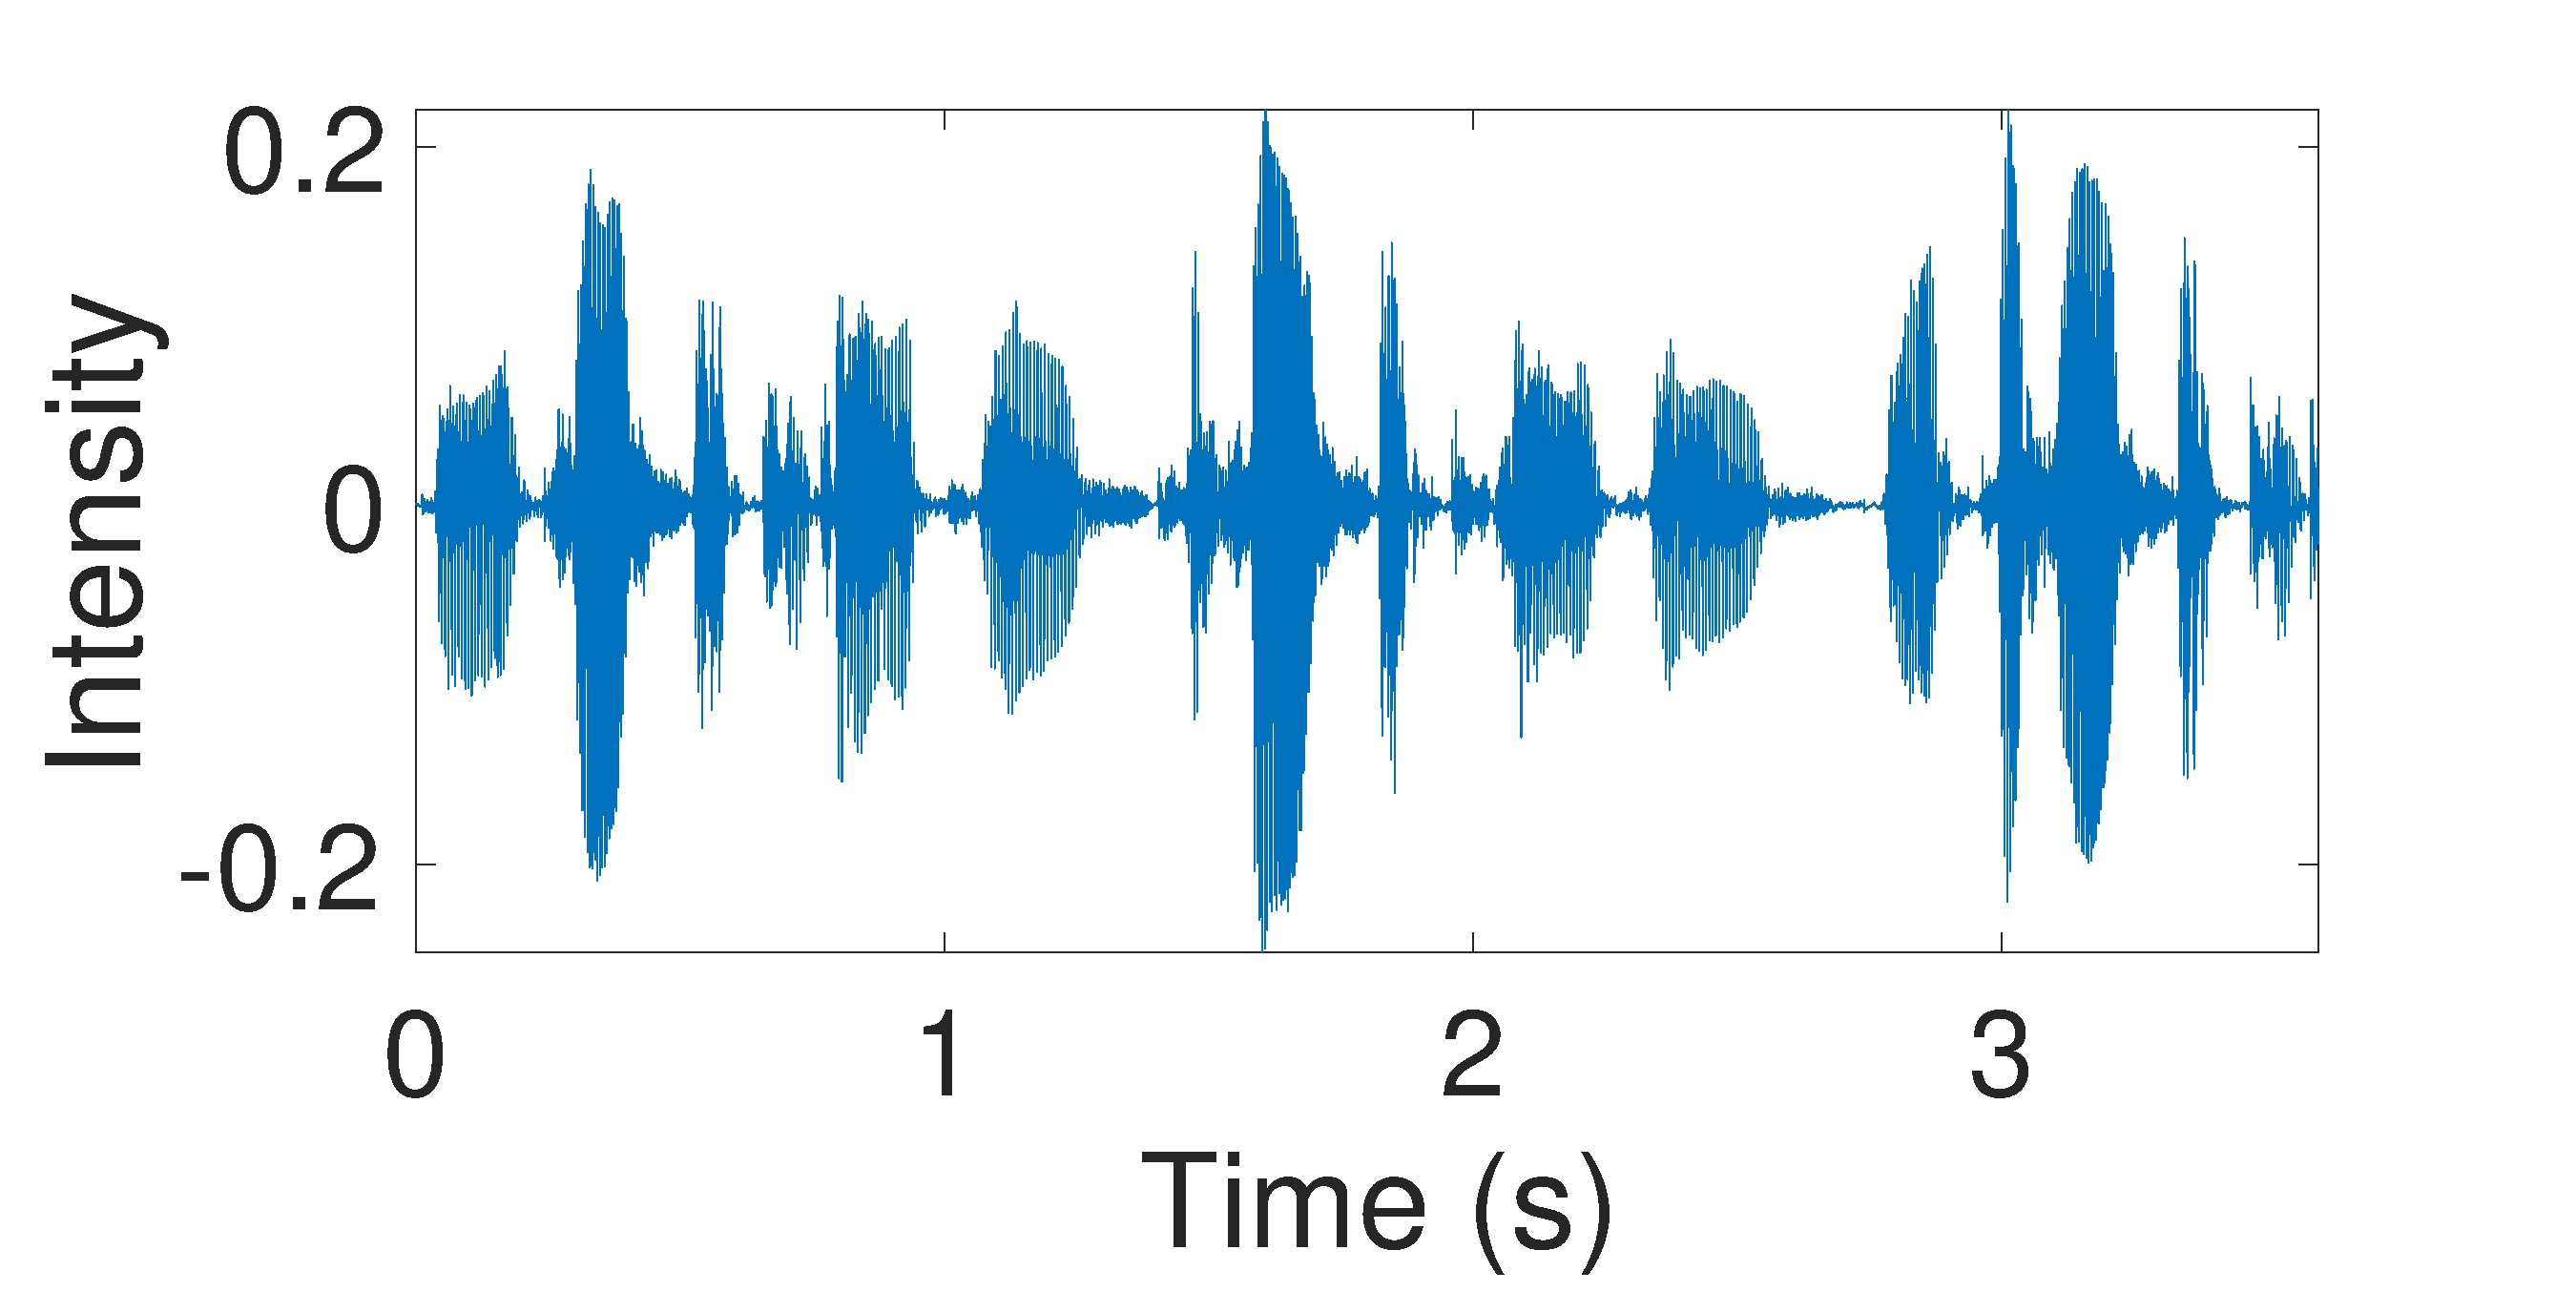
\includegraphics[width=\textwidth,trim=0.4cm 0cm 3.5cm 1.0cm,clip]
      {./sgp/pics/sound_data}
      \caption{Sound Data}
      \label{fig:sound_data}
    \end{subfigure}
    %
    \begin{subfigure}{0.47\textwidth}
      \centering
      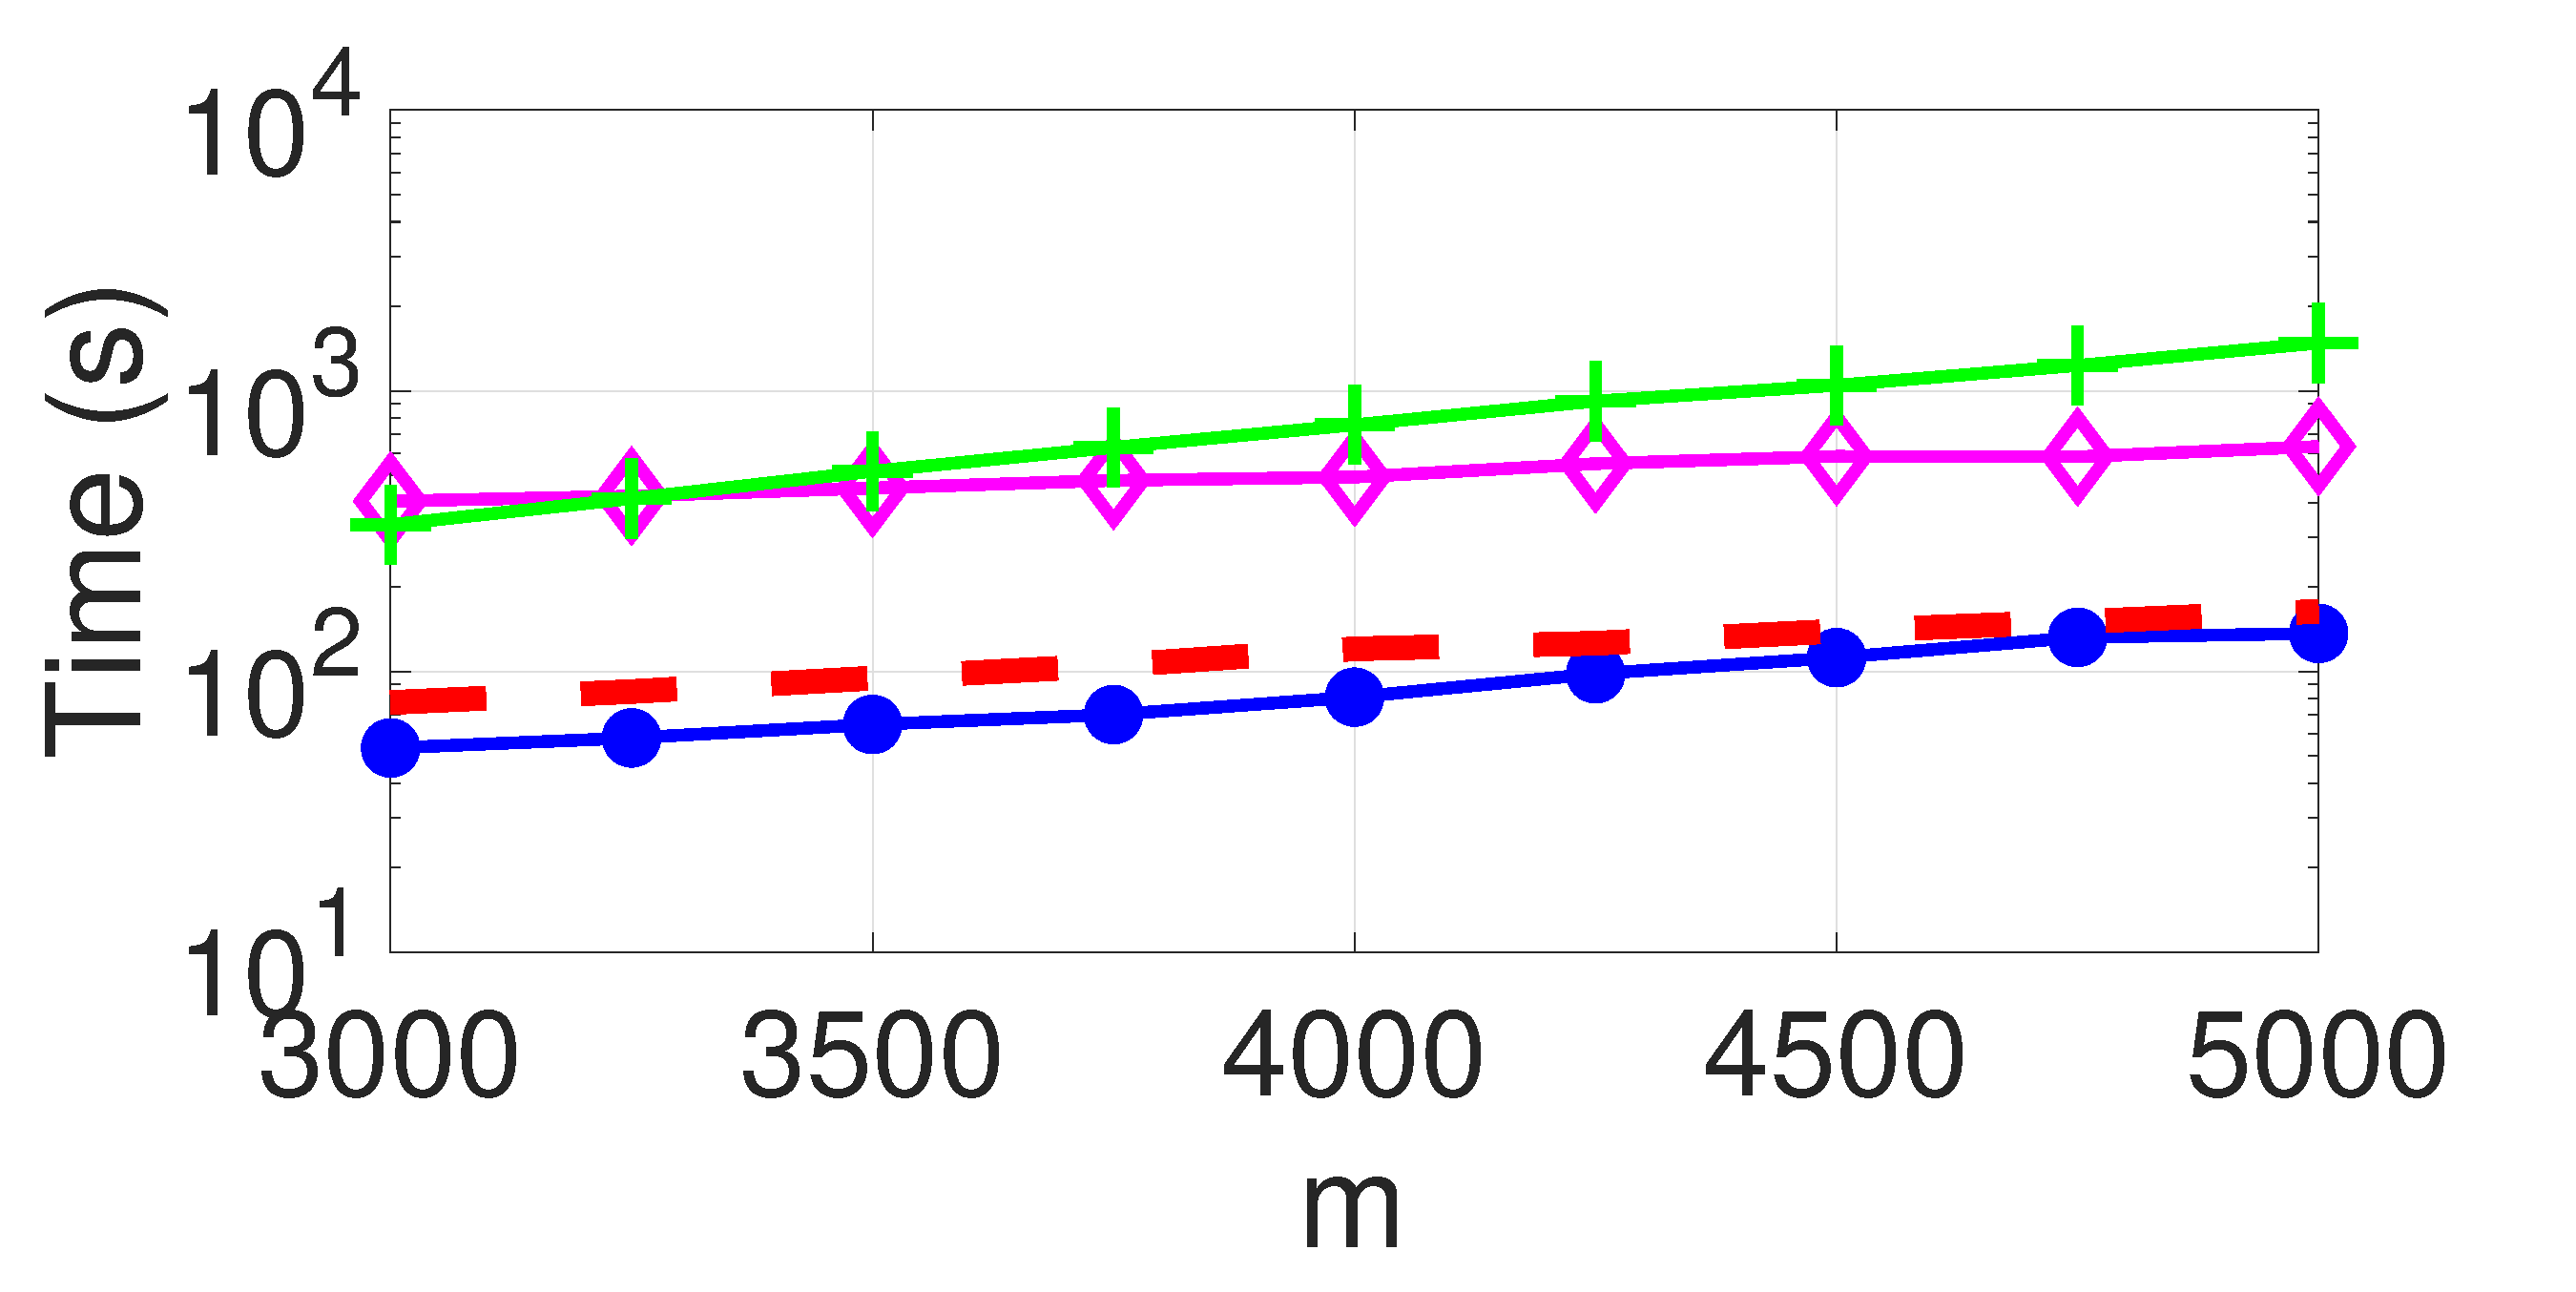
\includegraphics[width=\textwidth,trim=0.4cm 0cm 2.0cm 0cm,clip]
      {./sgp/pics/sound_recovery}
      \caption{Recovery Time}\label{fig:sound_recovery}
    \end{subfigure}
    %
    \begin{subfigure}{0.47\textwidth}
      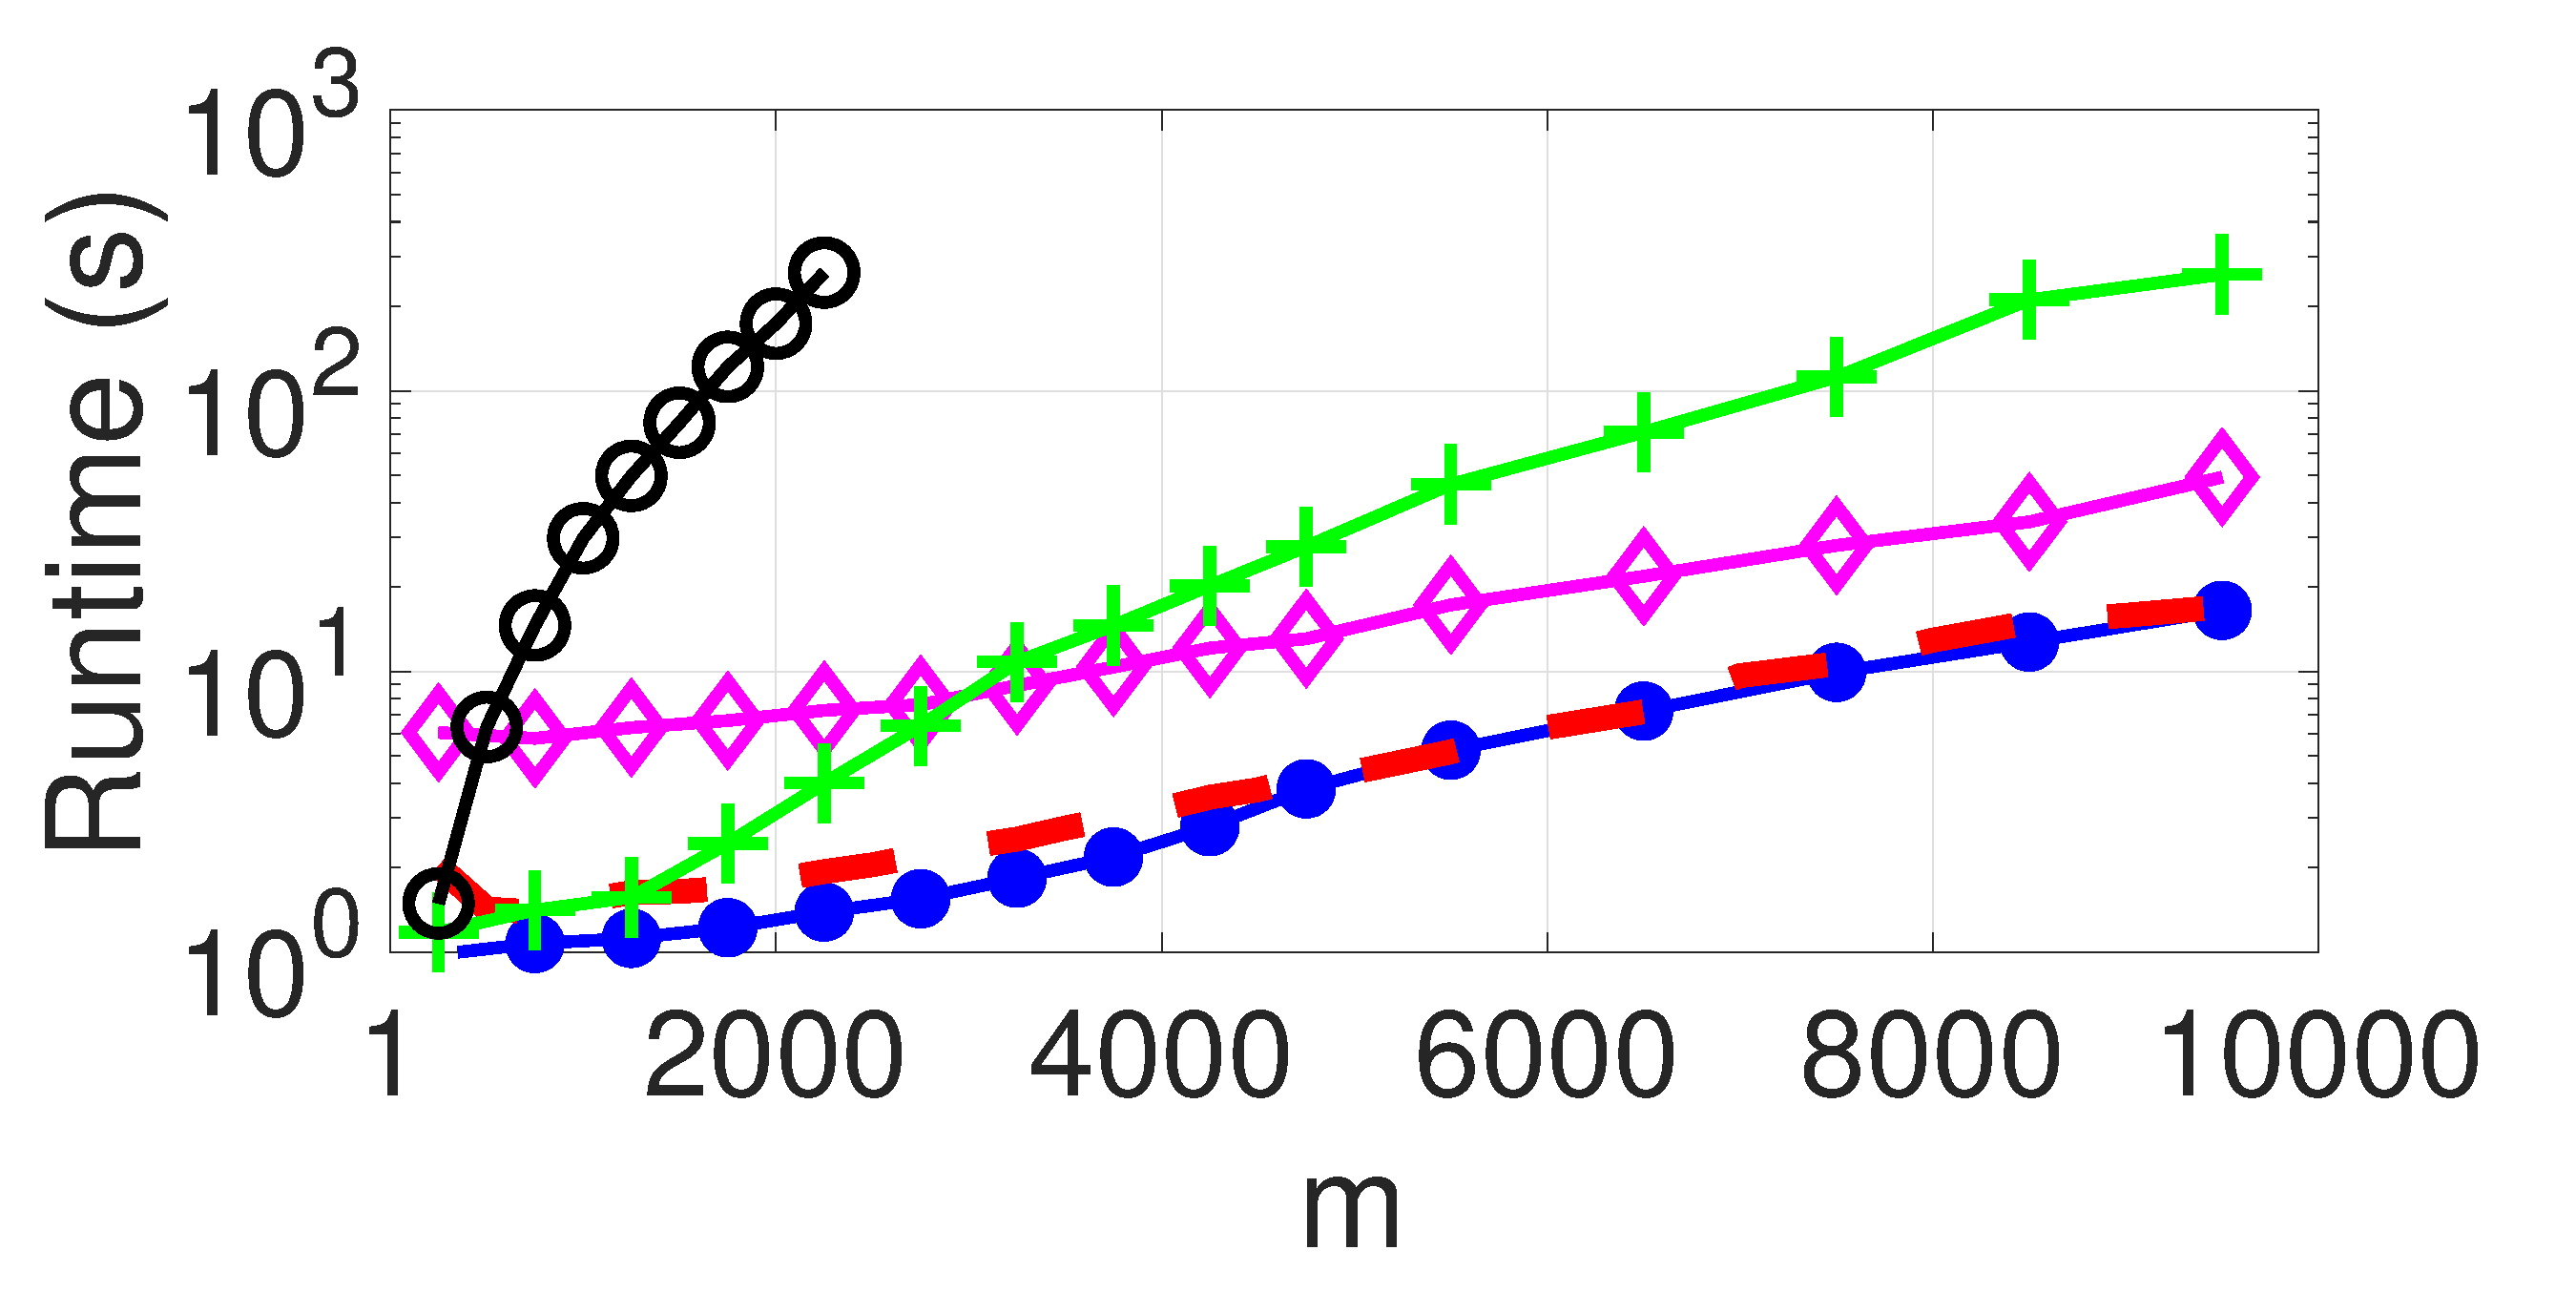
\includegraphics[width=\textwidth,trim=0.4cm 0cm 1.5cm 0.5cm,clip]
      {./sgp/pics/sound_inference}
      \caption{Inference Time}\label{fig:sound_inference}
    \end{subfigure}
    %
    \begin{subfigure}{0.47\textwidth}
      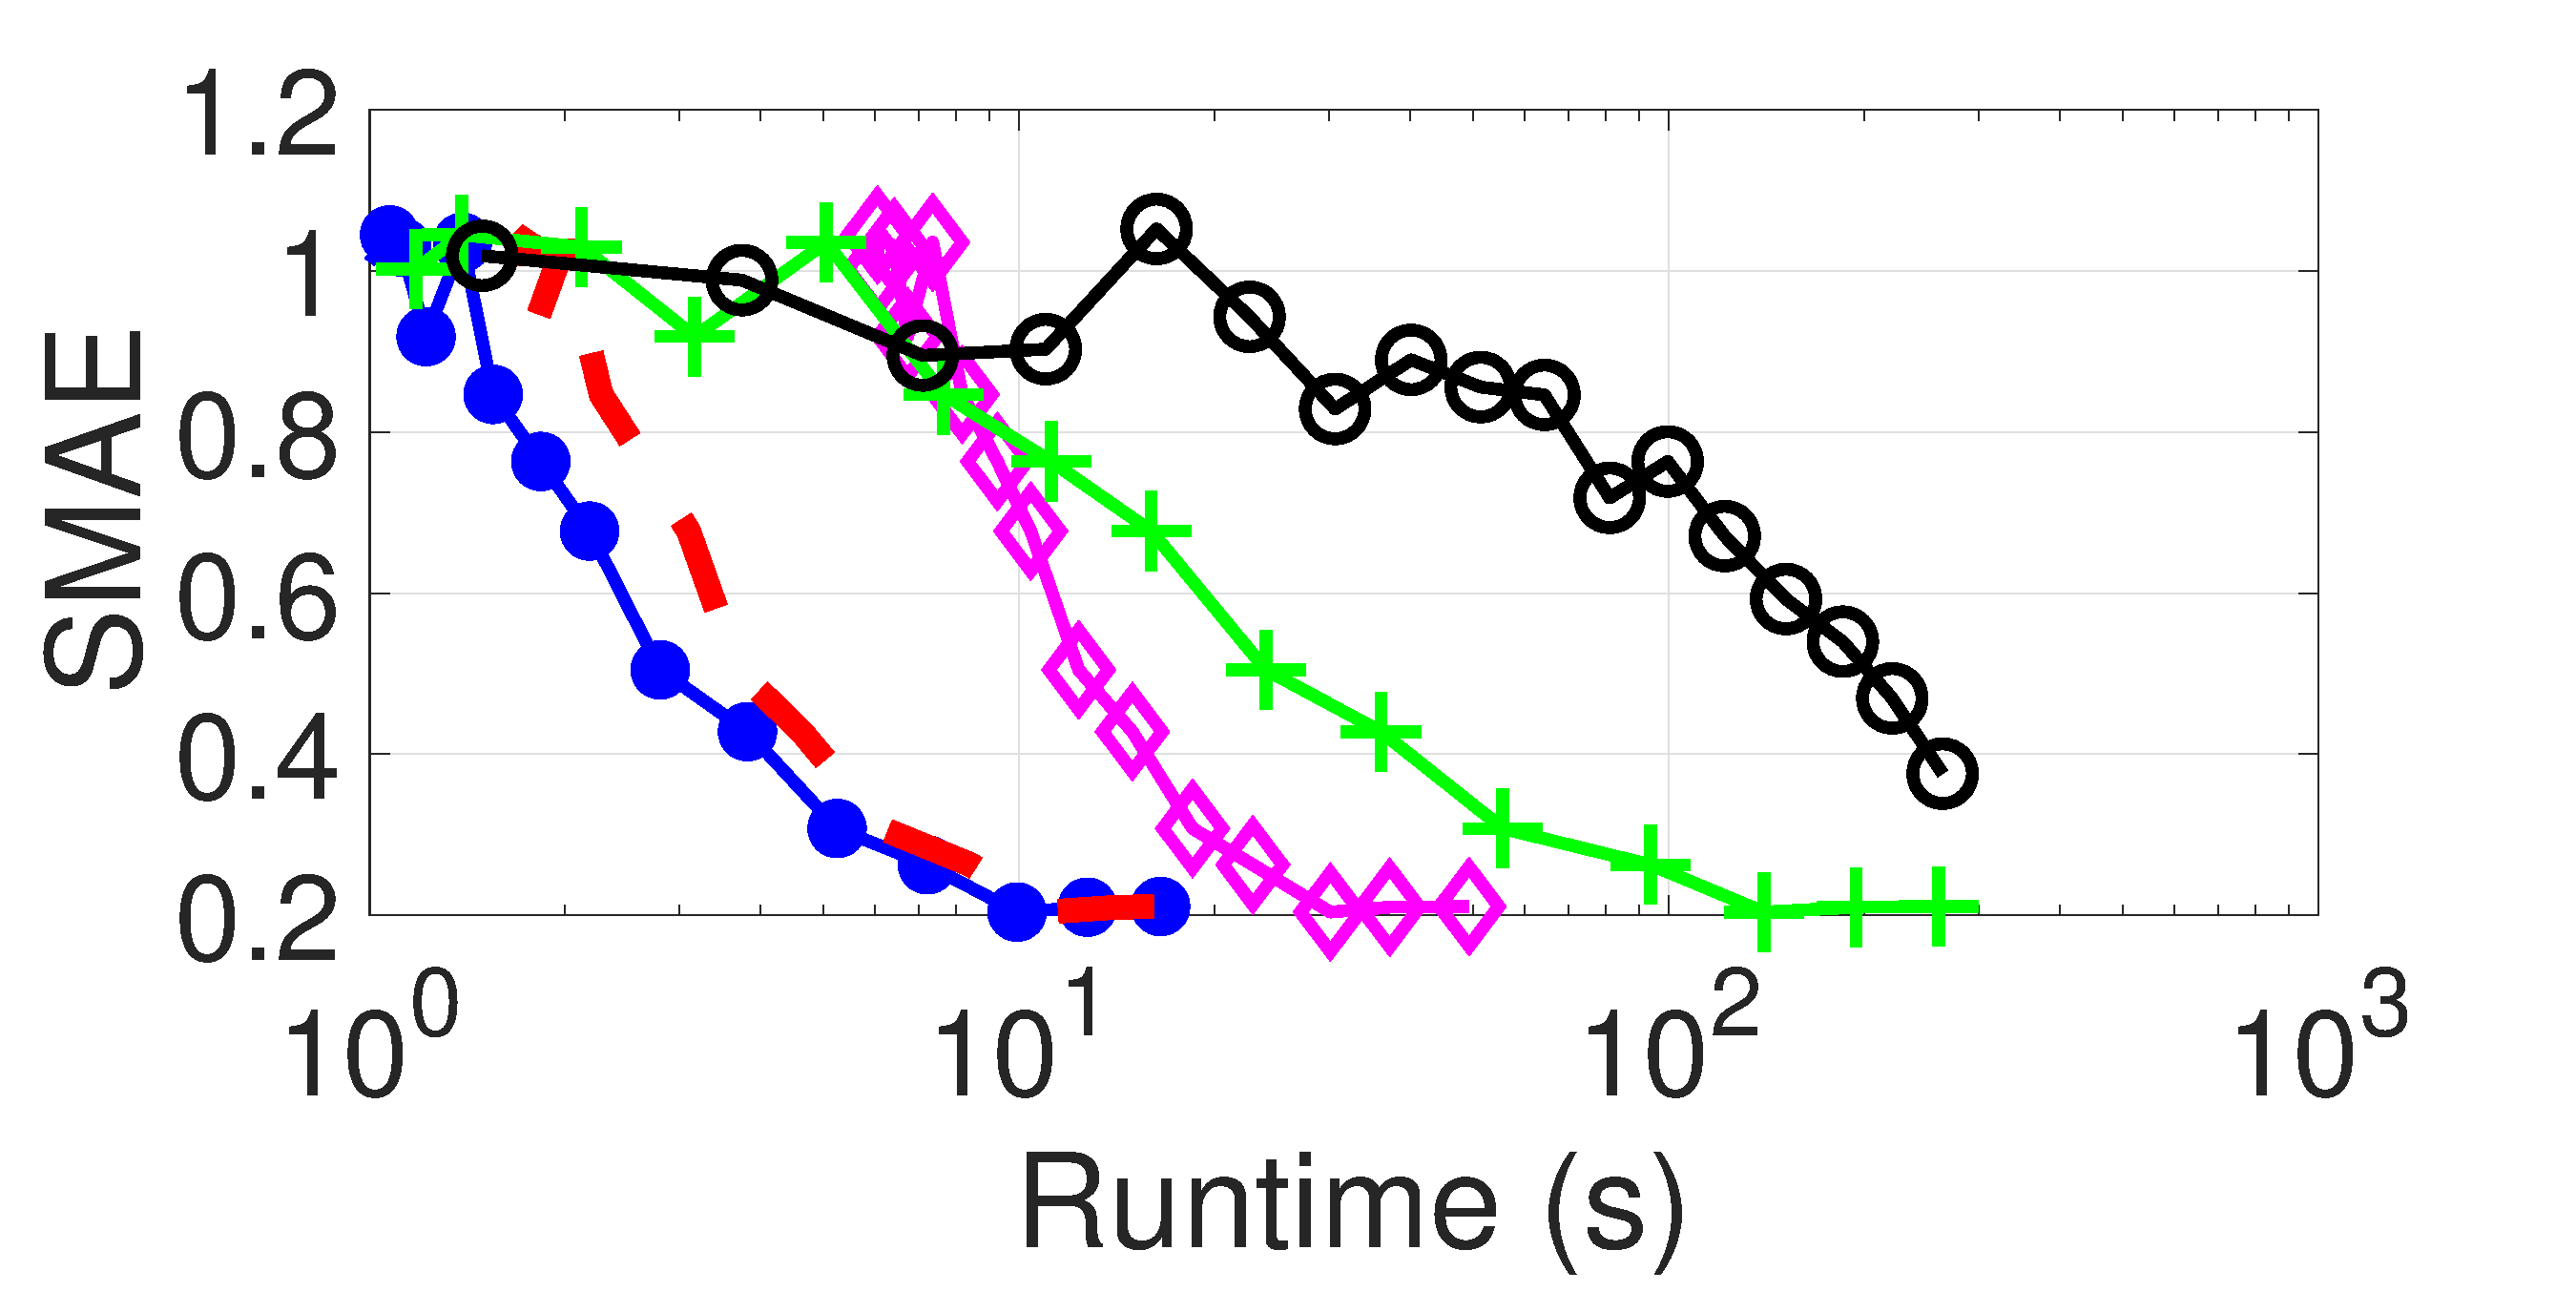
\includegraphics[width=\textwidth,trim=0.4cm 0cm 2.5cm 0.5cm,clip]
      {./sgp/pics/sound_smae}
      \caption{SMAE}\label{fig:sound_smae}
    \end{subfigure}
  \end{center}
  \caption{Sound modeling using 59,306 training points and 691 test points. The
  intensity of the time series can be seen in (a). Train time for RBF kernel
  hyper\hyp{}parameters is in (b) and the time for inference is in (c). The
  standardized mean absolute error (SMAE) as a function of time for an
  evaluation of the marginal likelihood and all derivatives is shown in (d).
  Surrogate is ({\color{blue} ------}), Lanczos is ({\color{red} - - -}),
  Chebyshev is {(\color{magenta} --- $\diamond$ ---}), scaled eigenvalues is ({
  \color{green} --- + ---}), and FITC is ({\color{black} --- o ---}).}
  \label{fig:sound_modeling}
\end{figure}

\subsection{Daily Precipitation Prediction}

This experiment involves precipitation data from the year of 2010 collected from
around $5500$ weather stations in the US\footnote{\url{https://catalog.data.gov/
dataset/u-s-hourly-precipitation-data}}. The hourly precipitation data is
preprocessed into daily data if full information of the day is available. The
dataset has $628,474$ entries in terms of precipitation per day given the date,
longitude and latitude. We randomly select $100,000$ data points as test points
and use the remaining points for training. We then perform hyper\hyp{}parameter
learning and prediction with the RBF kernel, using Lanczos, scaled eigenvalues,
and exact methods.

For Lanczos and scaled eigenvalues, we optimize the hyper\hyp{}parameters on the
subset of data for January 2010, with an induced grid of $100$ points per
spatial dimension and $300$ in the temporal dimension. Due to memory constraints
we only use a subset of $12,000$ entries for training with the exact method.
While scaled eigenvalues can perform well when fast eigendecompositions are
possible, as in this experiment, Lanczos nonetheless still runs faster and with
slightly lower mean square error (MSE).

\begin{table}[ht]
  \centering
  \caption{Prediction Comparison for the Daily Precipitation Data
  \textsuperscript{$\alpha$}.}\label{tab:precip}
  \begin{threeparttable}
    \begin{tabular}{r c c c c}
      \toprule
      Method  & \#Training Pts   & \#Induced Pts & MSE & Time [min]\\ \midrule
      Lanczos & 528k  & 3M  & 0.613 &  14.3\\
      Scaled\hyp{}Eig & 528k  & 3M  & 0.621 &  15.9\\
      Exact   & 12k   & -   & 0.903 &  11.8\\
      \bottomrule
    \end{tabular}
    \begin{tablenotes}
      \item[$\alpha$] The columns are the number of training points, number of
      induced grid points, mean squared error, and inference time.
    \end{tablenotes}
  \end{threeparttable}
\end{table}
Incidentally, we are able to use 3 \emph{million} inducing points in Lanczos and
scaled eigenvalues, which is enabled by the SKI representation 
\citep{wilson2015kernel} of covariance matrices, for a a very accurate
approximation.  This number of inducing points $M$ is unprecedented for typical
alternatives which scale as $\calO(M^3)$.

\subsection{Hickory Data}

In this experiment, we apply Lanczos to the log\hyp{}Gaussian Cox process model
with a Laplace approximation for the posterior distribution. We use the RBF
kernel and the Poisson likelihood in our model.  The scaled eigenvalue method
does not apply directly to non\hyp{}Gaussian likelihoods; we thus applied the
scaled eigenvalue method in \citep{wilson2015kernel} in conjunction with the
Fiedler bound in \citep{flaxman2015fast} for the scaled eigenvalue comparison. 
Indeed, a key advantage of the Lanczos approach is that it can be applied
whenever fast MVMs are available, which means no additional approximations such
as the Fiedler bound are required for non\hyp{}Gaussian likelihoods.

This dataset, which comes from the R package {\tt spatstat}, is a point pattern
of $703$ hickory trees in a forest in Michigan. We discretize the area into a
$60 \times 60$ grid and fit our model with exact, scaled eigenvalues, and
Lanczos. We see in Table \ref{tab:hickory} that Lanczos recovers
hyper\hyp{}parameters that are much closer to the exact values than the scaled
eigenvalue approach. \cref{fig:hickory} shows that the predictions by Lanczos
are also indistinguishable from the exact computation.

\begin{table}[ht]
  \centering
  \caption{Hyperparameters Recovered on the Hickory Dataset.}\label{tab:hickory}
  \begin{tabular}{r c c c c c}
    \toprule
    Method & $s_f$ & $\ell_1$ & $\ell_2$ & $-\log p(y|\theta)$ & Time [s]\\
    \midrule
    Exact & $0.696$  & $0.063$  & $0.085$ &  $1827.56$ & $465.9$\\
    Lanczos & $0.693$   & $0.066$   & $0.096$ &  $1828.07$ & $21.4$\\
    Scaled\hyp{}Eig & $0.543$  & $0.237$  & $0.112$ &  $1851.69$ & $2.5$\\
    \bottomrule
  \end{tabular}
\end{table}
\vfill

\begin{figure}[ht]
  \begin{center}
    \begin{subfigure}{0.3\textwidth}
      \centering
      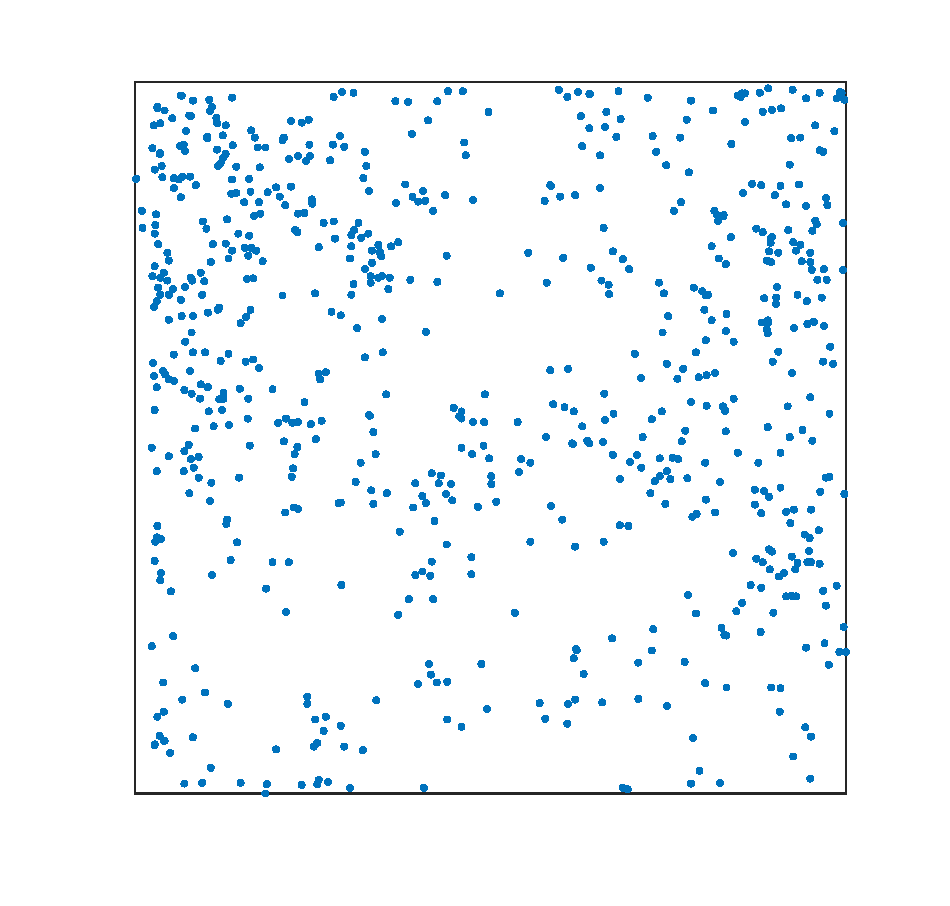
\includegraphics[height=0.87\textwidth,trim = 1cm 1cm 1cm 1cm,clip]
      {./sgp/pics/Hickory_point.eps}
      \caption{Point Pattern Data}\label{fig:hpoint}
    \end{subfigure}
    \hspace{1cm}
    \begin{subfigure}{0.3\textwidth}
      \centering
      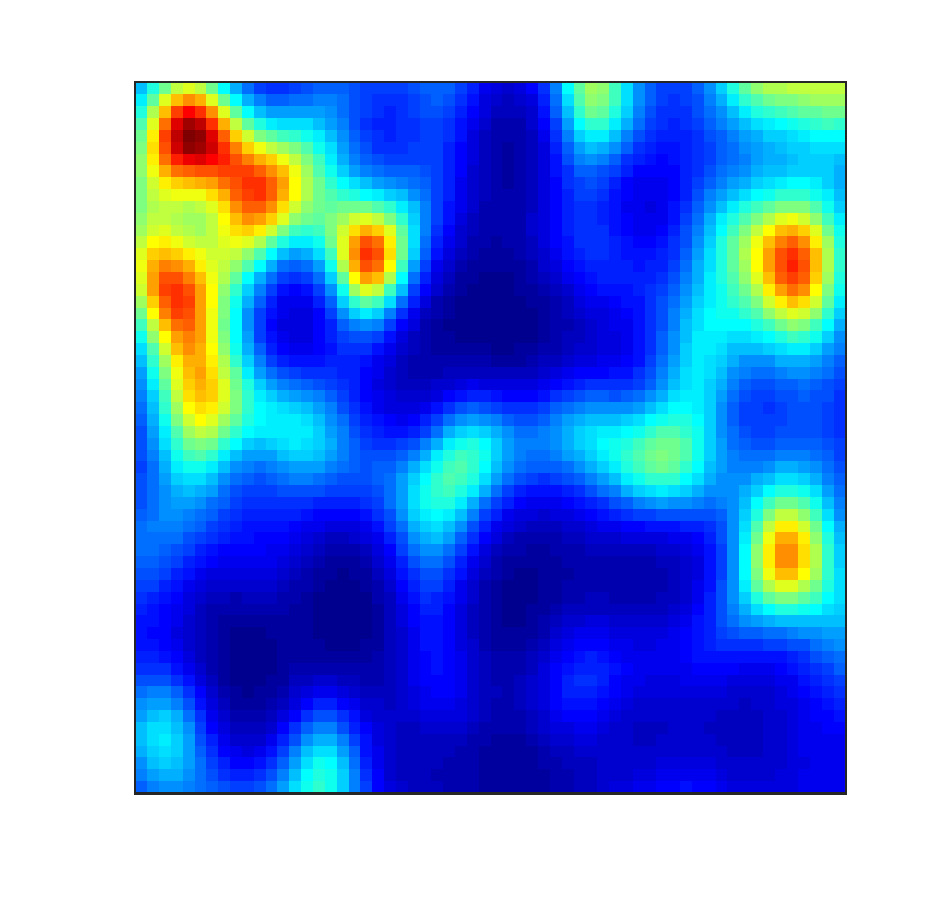
\includegraphics[height=0.87\textwidth,trim = 1cm 1cm 1cm 1cm,clip]
      {./sgp/pics/Hickory_exact.eps}
      \caption{Prediction by Exact}\label{fig:hickory_exact}
    \end{subfigure}
    \linebreak
    \begin{subfigure}{0.3\textwidth}
      \centering
      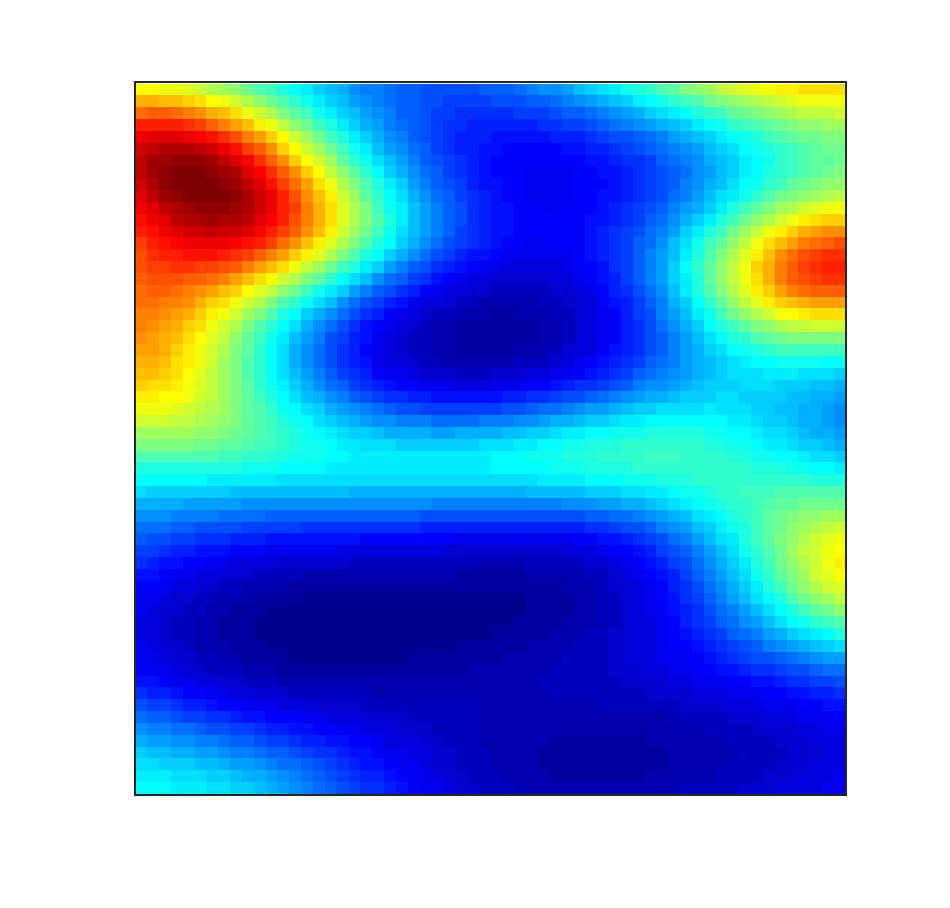
\includegraphics[height=0.87\textwidth,trim = 1cm 1cm 1cm 1cm,clip]
      {./sgp/pics/Hickory_ski.eps}
      \caption{Scaled\hyp{}Eig}\label{fig:hickory_ski}
    \end{subfigure}
    \hspace{1cm}
    \begin{subfigure}{0.3\textwidth}
      \centering
      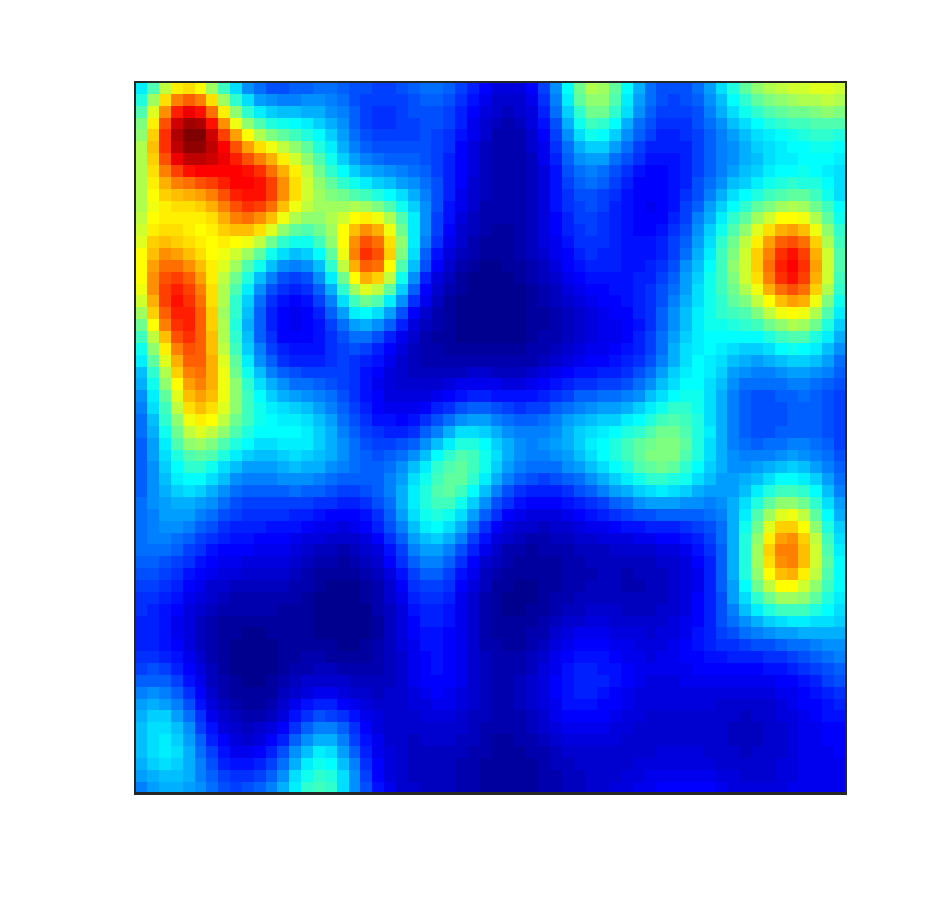
\includegraphics[height=0.87\textwidth,trim = 1cm 1cm 1cm 1cm,clip]
      {./sgp/pics/Hickory_lan.eps}
      \caption{Lanczos}\label{fig:hickory_lan}
    \end{subfigure}
    \caption{Predictions by exact, scaled eigenvalues, and Lanczos on the Hickory dataset.}\label{fig:hickory}
  \end{center}
\end{figure}

\subsection{Crime Prediction}

In this experiment, we apply Lanczos with the spectral mixture kernel to the
crime forecasting problem considered in \cite{flaxman2015fast}. This dataset
consists of $233,088$ incidents of assault in Chicago from January 1, 2004 to
December 31, 2013. We use the first $8$ years for training and attempt to
predict the crime rate for the last $2$ years. For the spatial dimensions, we
use the log\hyp{}Gaussian Cox process model, with the Mat\'ern\hyp{}5/2 kernel,
the negative binomial likelihood, and the Laplace approximation for the
posterior. We use a spectral mixture kernel with $20$ components and an extra
constant component for the temporal dimension. We discretize the data into a $17
\times 26$ spatial grid corresponding to $1\mile\Times1\mile$ grid cells. In
the temporal dimension we sum our data by weeks for a total of $522$ weeks.
After removing the cells that are outside Chicago, we have a total of $157,644$
observations.

The results for Lanczos and scaled eigenvalues (in conjunction with the Fiedler
bound due to the non\hyp{}Gaussian likelihood) can be seen in 
\cref{tab:chicago_homicide}. The Lanczos method used $5$ Hutchinson probe vectors
and $30$ Lanczos steps. For both methods we allow $100$ iterations of LBFGS to
recover hyper\hyp{}parameters and we often observe early convergence. While the
root mean square error (RMSE) for Lanczos and scaled eigenvalues happen to be
close on this example, the recovered hyper\hyp{}parameters using scaled
eigenvalues are very different than for Lanczos. For example, the scaled
eigenvalue method learns much larger $\sigma^2$ than Lanczos, indicating model
misspecification. In general, as the data become increasingly non\hyp{}Gaussian
the Fiedler bound (used for fast scaled eigenvalues on non\hyp{}Gaussian
likelihoods) will become increasingly misspecified, while Lanczos will be
unaffected.

\begin{table}[ht]
  \centering
  \caption{Hyperparameters Recovered, Recovery Time and RMSE for Lanczos and
  Scaled Eigenvalues on the Chicago Assault Data\textsuperscript{$\alpha$}.}
  \label{tab:chicago_homicide}
  \begin{threeparttable}
    \begin{tabular}{r c c c c c c c}
      \toprule
      Method & $\ell_1$ & $\ell_2$ & $\sigma^2$ & T\textsubscript{recovery}[s]&
      T\textsubscript{prediction}[s] & RMSE\textsubscript{train} &
      RMSE\textsubscript{test} \\
      \midrule
      Lanczos & 0.65 & 0.67 & \ph69.72 & 264 & 10.30 & 1.17 & 1.33 \\
      Scaled\hyp{}Eig & 0.32 & 0.10 & 191.17 & \ph67 & \ph3.75 & 1.19 & 1.36 \\
      \bottomrule
    \end{tabular}
    \begin{tablenotes}
      \item[$\alpha$] $\ell_1$ and $\ell_2$ are the length scales in
      spatial dimensions. $\sigma^2$ is the noise level.
      T\textsubscript{recovery} is the time for recovering hyper
      \hyp{}parameters. T\textsubscript{prediction} is the time for prediction
      at all $157,644$ observations, including training and testing.
    \end{tablenotes}
  \end{threeparttable} 
\end{table}

\subsection{Deep Kernel Learning}
To handle high\hyp{}dimensional datasets, we bring our methods into the deep
kernel learning framework \cite{wilson2016deep} by replacing the final layer of
a pre\hyp{}trained deep neural network (DNN) with a GP. This experiment uses the
gas sensor dataset from the UCI machine learning repository. It has $2565$
instances with $128$ dimensions. We pre\hyp{}train a DNN, then attach a Gaussian
process with RBF kernels to the two\hyp{}dimensional output of the
second\hyp{}to\hyp{}last layer. We then further train all parameters of the
resulting kernel, \emph{including} the weights of the DNN, through the GP
marginal likelihood. In this example, Lanczos and the scaled eigenvalue approach
perform similarly well.  Nonetheless, we see that Lanczos can effectively be
used with SKI on a high dimensional problem to train hundreds of thousands of
kernel parameters.

\begin{table}[ht]
  \centering
  \caption{Prediction RMSE and Per Training Iteration Runtime.}\label{tab:dkl}
  \begin{tabular}{r c c c}
    \toprule
    Method & DNN & Lanczos & Scaled\hyp{}Eig \\
    \midrule
    RMSE & $0.1366\pm 0.0387$ & $0.1053\pm0.0248$ & $0.1045\pm 0.0228$\\
    Time [s]& $0.4438$ & $2.0680$ & $1.6320$\\
    \bottomrule
  \end{tabular} 
\end{table}

\subsection{1D Cross-section Plots}\label{sup:1dcross}

In this experiment we compare the accuracy of Lanczos and Chebyshev for
1\hyp{}dimensional perturbations of a set of true hyper\hyp{}parameters,
and demonstrate how critical it is to use diagonal replacement for some
approximate kernels. We choose the true hyper\hyp{}parameters to be $
(\ell,s_f,\sigma) = (0.1,1,0.1)$ and consider two different types of datasets.
The first dataset consists of $1000$ equally spaced points in the interval $
[0,4]$ in which case the kernel matrix of a stationary kernel is Toeplitz and we
can make use of fast matrix\hyp{}vector multiplication. The second dataset
consists of $1000$ data points drawn independently from a
$U(0,4)$ distribution. We use SKI with cubic interpolation to construct an
approximate kernel based on $1000$ equally spaced points. The function values
are drawn from a GP with the true hyper\hyp{}parameters, for both the true and
approximate kernel. We use $250$ iterations for Lanczos and $250$ Chebyshev
moments in order to assure convergence of both methods. The results for the
first dataset with the RBF and Mat\'ern kernels can be seen in 
\crefrange{fig:1dpert_a}{fig:1dpert_d}. The results for the second
dataset with the SKI kernel can be seen in 
\crefrange{fig:1dpert_kissgp_a}{fig:1dpert_kissgp_d}.

\begin{figure}[ht]
  \begin{center}
    \begin{subfigure}{0.46\textwidth}
      \centering
      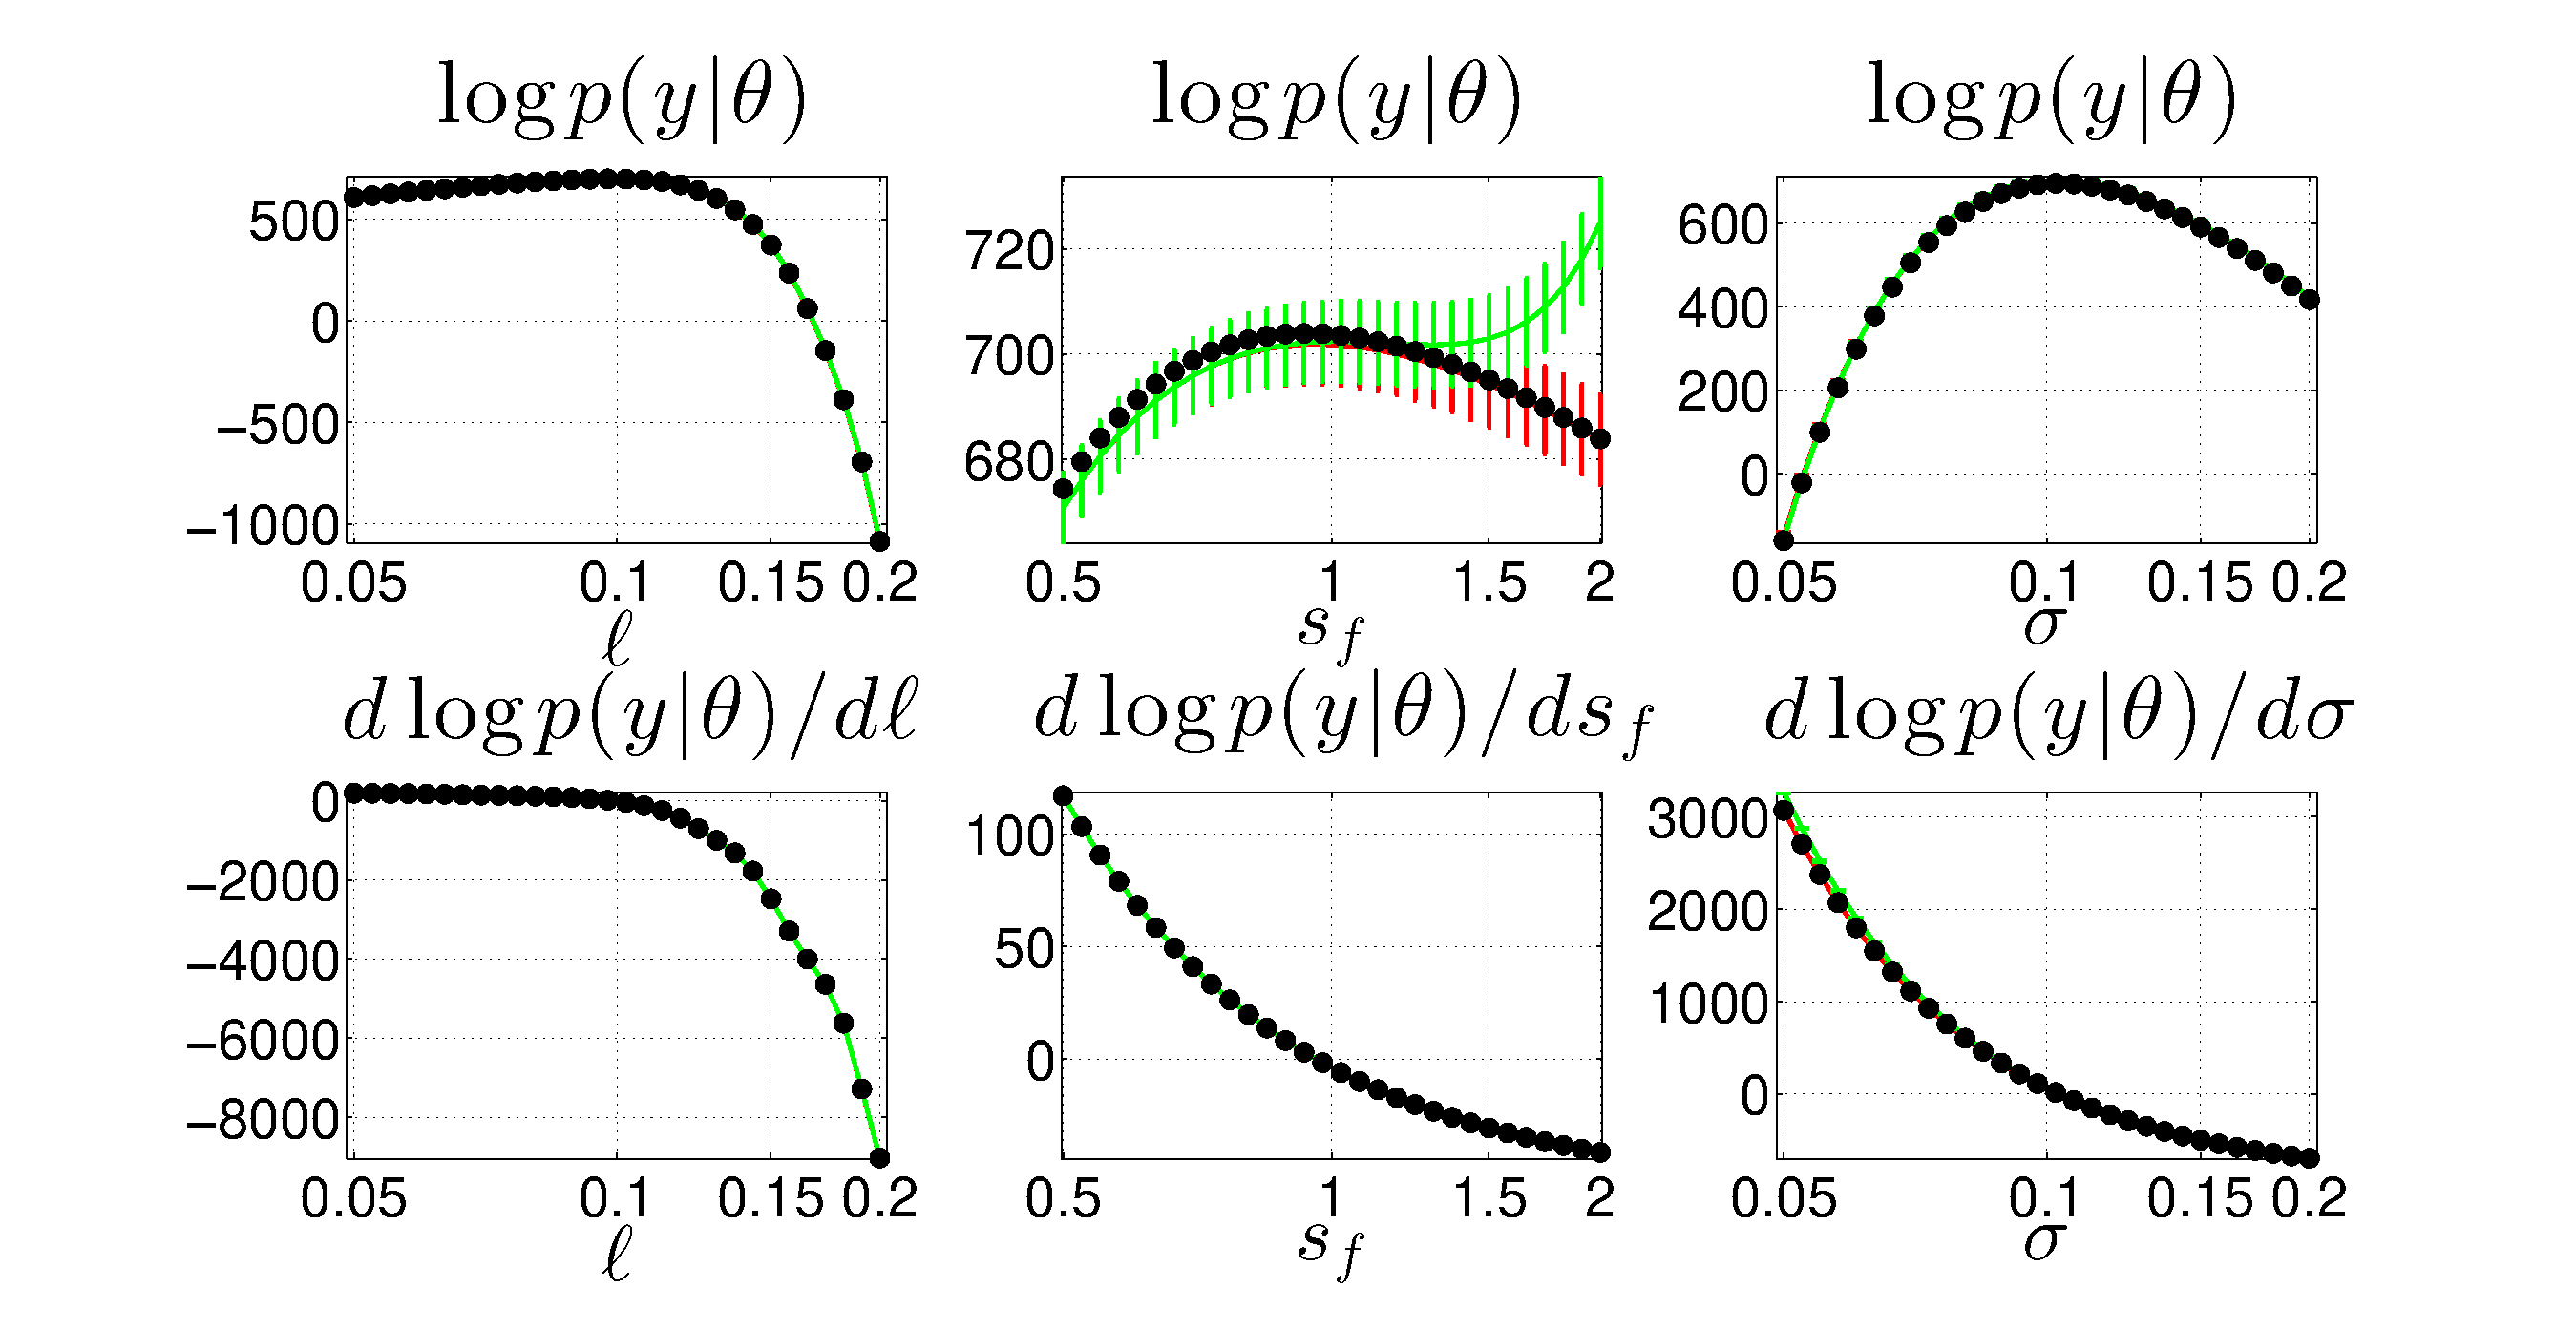
\includegraphics[width=\textwidth,trim=3.5cm 0cm 3.5cm 0cm,clip]
      {./sgp/pics/loglik_rbf}
      \caption{Log marginal likelihood for the RBF \\kernel}\label{fig:1dpert_a}
    \end{subfigure}
    \begin{subfigure}{0.46\textwidth}
      \centering
      \includegraphics[width=\textwidth,trim=3.5cm 0cm 3.5cm 0cm,clip]
      {./sgp/pics/loglik_Matern}
      \caption{Log marginal likelihood for the Mat\'ern \\kernel}
      \label{fig:1dpert_b}
    \end{subfigure}
    \begin{subfigure}{0.46\textwidth}
      \centering
      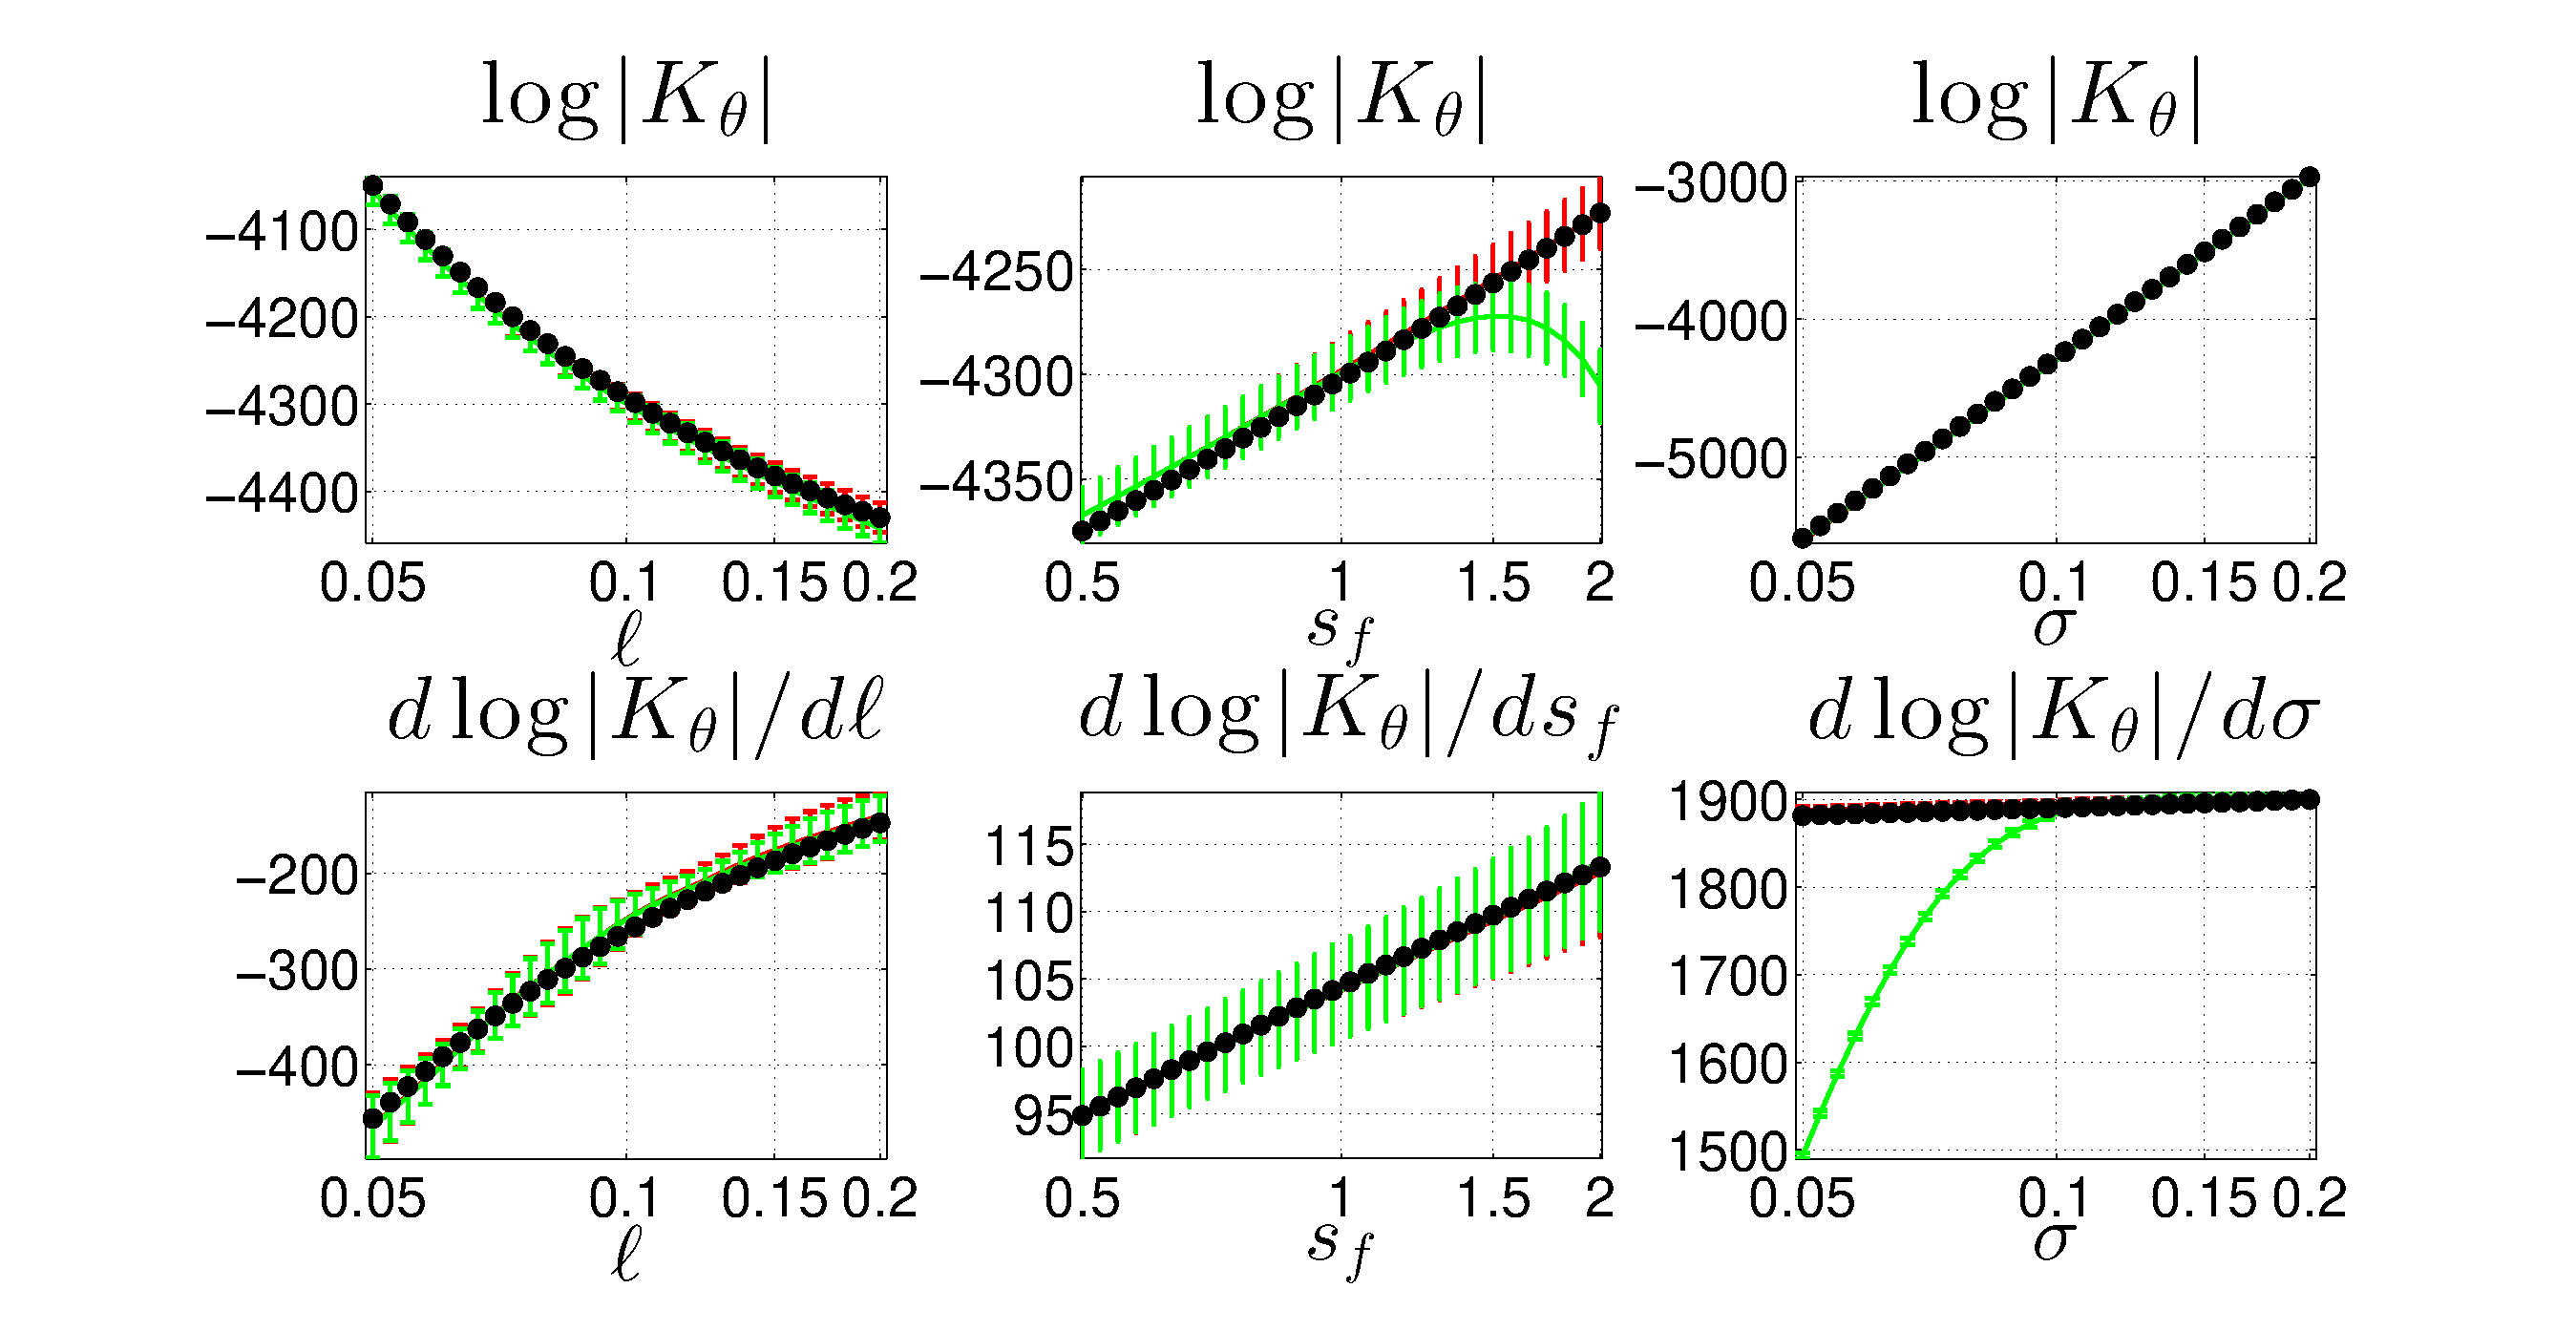
\includegraphics[width=\textwidth,trim=3.5cm 0cm 3.5cm 0cm,clip]
      {./sgp/pics/logdet_rbf}
      \caption{Log determinant for the RBF kernel}\label{fig:1dpert_c}
    \end{subfigure}
    \begin{subfigure}{0.46\textwidth}
      \centering
      \includegraphics[width=\textwidth,trim=3.5cm 0cm 3.5cm 0cm,clip]
      {./sgp/pics/logdet_Matern}
      \caption{Log determinant for the Mat\'ern kernel}\label{fig:1dpert_d}
    \end{subfigure}
    \caption{1\hyp{}dimensional perturbations for the exact RBF and 
    Mat\'ern\hyp{}1/2 kernel where the data is $1000$ equally spaced points in
    the interval $[0,4]$. The exact values are ($\bullet$), Lanczos is ({
    \color{red}-----}), Chebyshev is ({\color{green}-----}). The error bars of
    Lanczos and Chebyshev are $1$ standard deviation and were computed from $10$
    runs with different probe vectors}\label{fig:1dpert}
  \end{center}
\end{figure}

\begin{figure}[ht]
  \begin{center}
    \begin{subfigure}{0.46\textwidth}
      \centering
      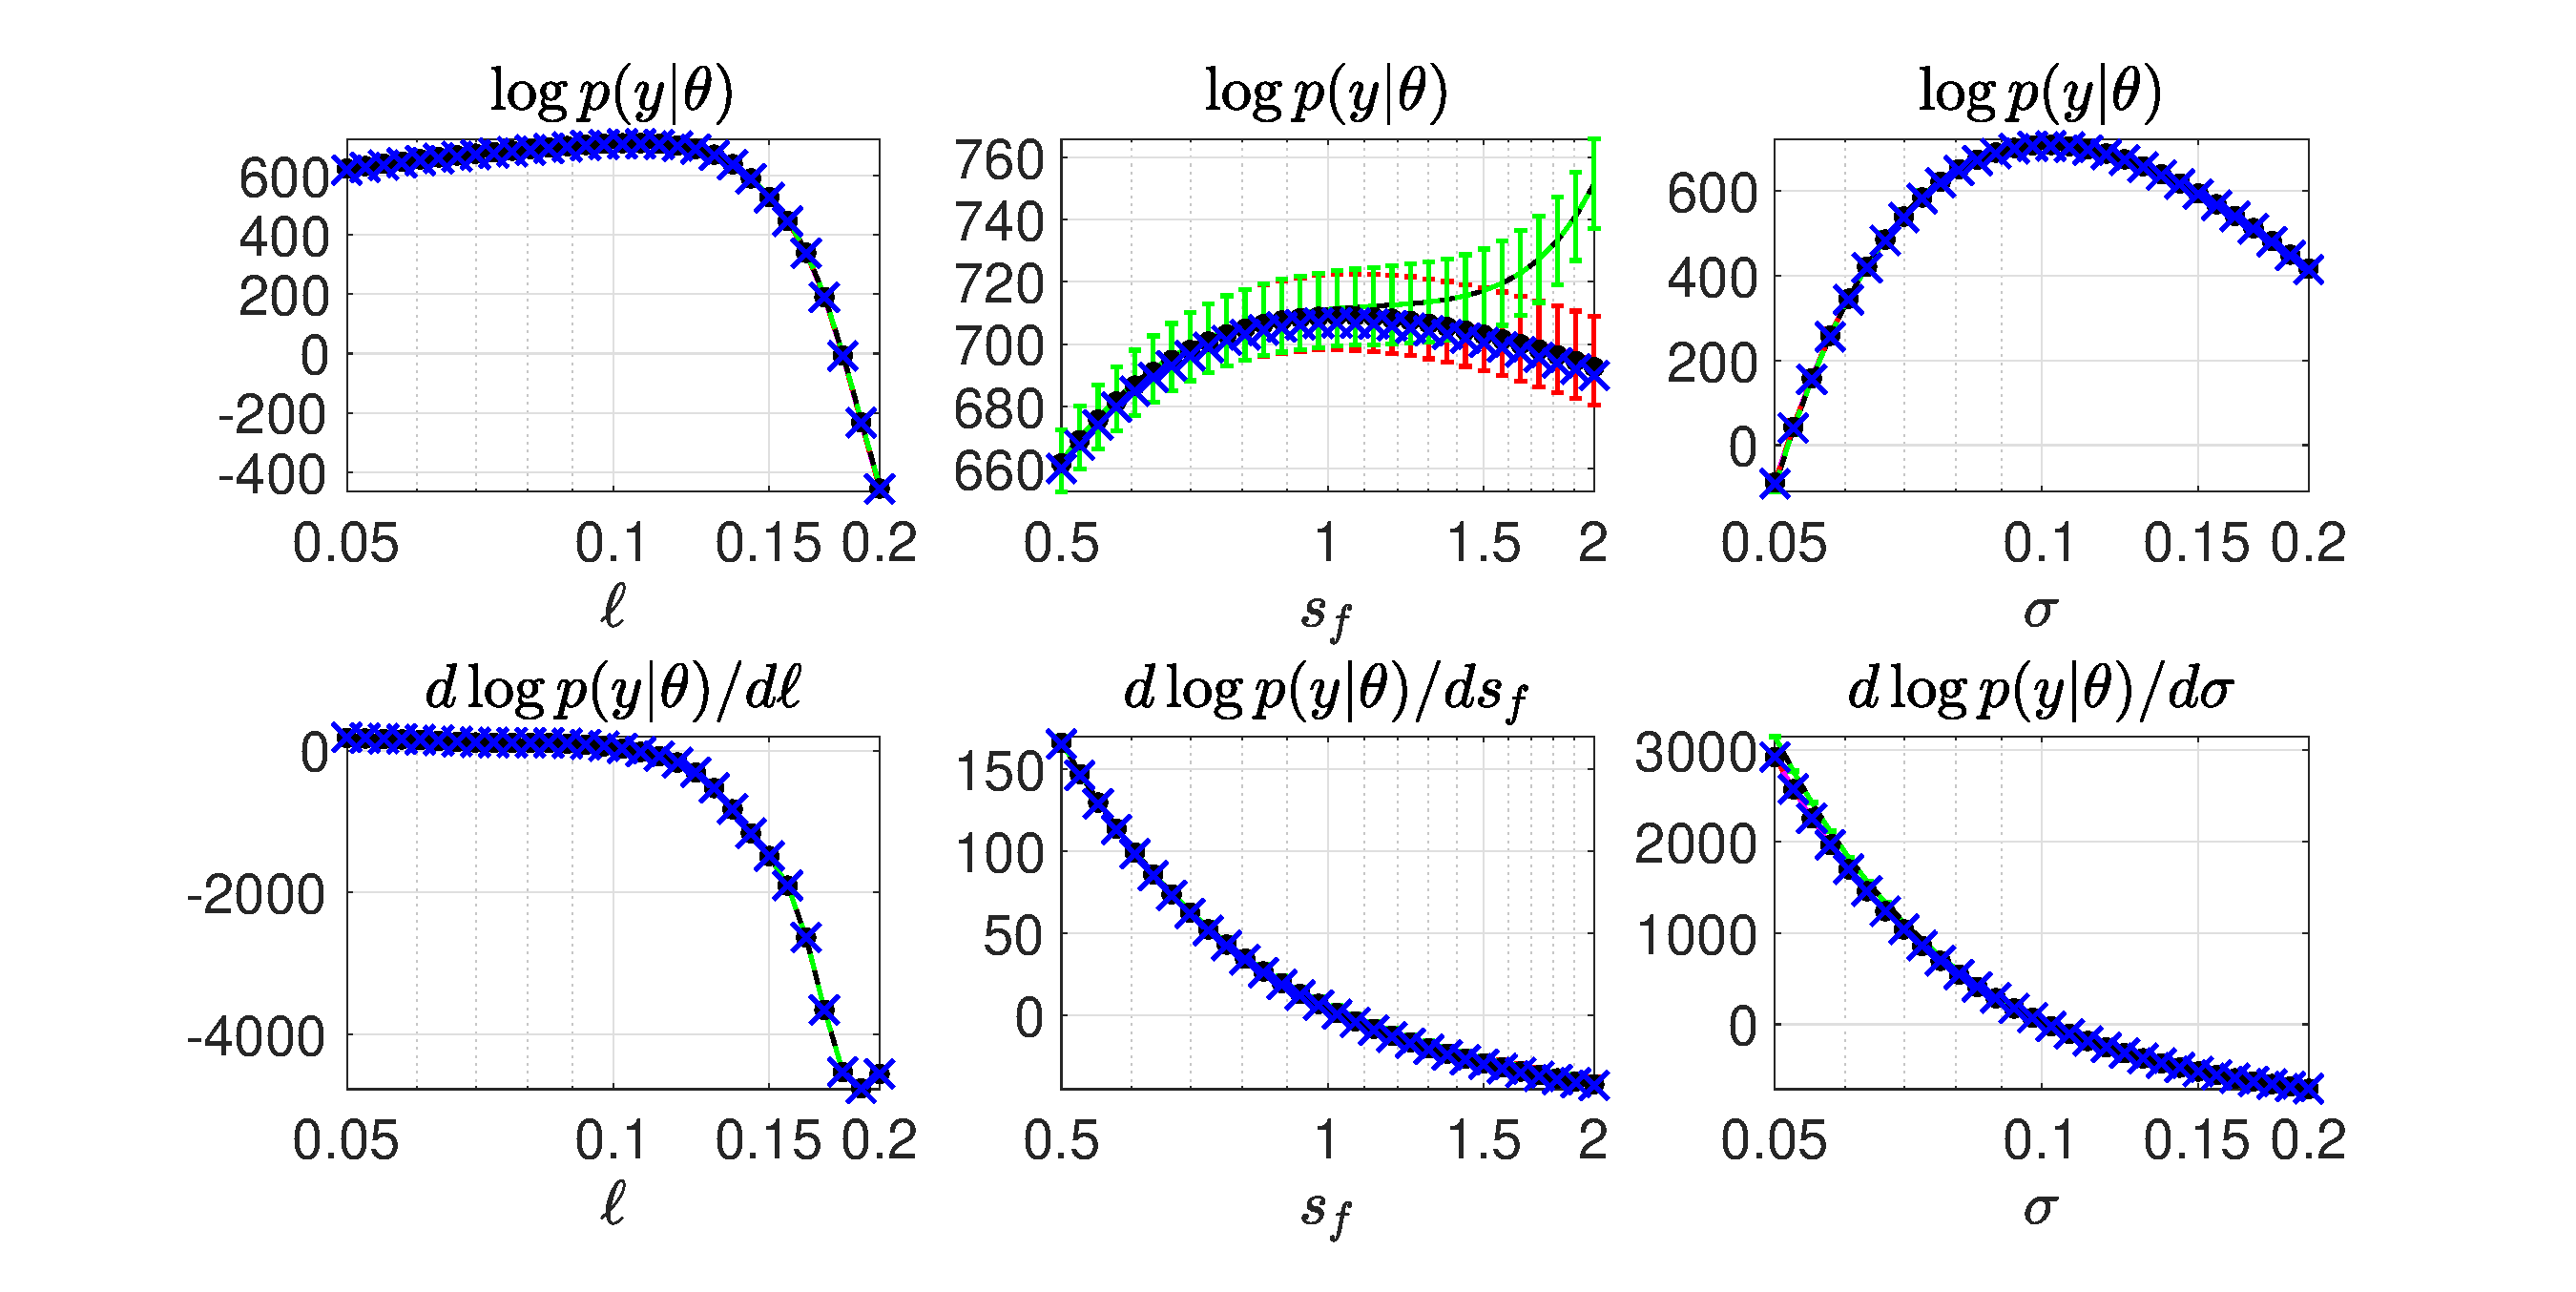
\includegraphics[width=\textwidth,trim=2.5cm 0cm 3.5cm 0cm,clip]
      {./sgp/pics/loglik_rbf_apx}
      \caption{Log marginal likelihood for the RBF \\kernel}
      \label{fig:1dpert_kissgp_a}
    \end{subfigure}
    \begin{subfigure}{0.46\textwidth}
      \centering
      \includegraphics[width=\textwidth,trim=2.5cm 0cm 3.5cm 0cm,clip]
      {./sgp/pics/loglik_matern_apx}
      \caption{Log marginal likelihood for the Mat\'ern \\kernel}
      \label{fig:1dpert_kissgp_b}
    \end{subfigure}
    \begin{subfigure}{0.46\textwidth}
      \centering
      \includegraphics[width=\textwidth,trim=2.5cm 0cm 3.5cm 0cm,clip]
      {./sgp/pics/logdet_rbf_apx}
      \caption{Log determinant for the RBF kernel}
      \label{fig:1dpert_kissgp_c}
    \end{subfigure}
    \begin{subfigure}{0.46\textwidth}
      \centering
      \includegraphics[width=\textwidth,trim=2.5cm 0cm 3.5cm 0cm,clip]
      {./sgp/pics/logdet_matern_apx}
      \caption{Log determinant for the Mat\'ern kernel}
      \label{fig:1dpert_kissgp_d}
    \end{subfigure}
    \caption{1\hyp{}dimensional perturbations with the SKI (cubic)
    approximations of the RBF and Mat\'ern\hyp{}1/2 kernel where the data is
    1000 points drawn from $\calN(0,2)$. The exact values are ($\bullet$),
    Lanczos with diagonal replacement is ({\color{red}-----}), Chebyshev with
    diagonal replacement is ({\color{green}-----}), Lanczos without diagonal
    replacement is ({\color{magenta}-----}), Chebyshev without diagonal
    replacement is ({\color{black}-----}), and scaled eigenvalues is ({
    \color{blue} $\times$}). Diagonal replacement makes no perceptual difference
    for the RBF kernel so the lines are overlapping in this case. The error bars
    of Lanczos and Chebyshev are $1$ standard deviation and were computed from
    $10$ runs with different probe vectors}\label{fig:1dpert_kissgp}
 \end{center}
\end{figure}

Lanczos yields an excellent approximation to the log determinant and its
derivatives for both the exact and the approximate kernels, while Chebyshev
struggles with large values of $s_f$ and small values of $\sigma$ on the
exact and approximate RBF kernel. This is expected since Chebyshev has issues
with the singularity at zero while Lanczos has large quadrature weights
close to zero to compensate for this singularity. The scaled eigenvalue method
has issues with the approximate Mat\'ern\hyp{}1/2 kernel.

\subsection{Why Lanczos is Better Than Chebyshev}\label{sup:lanczoscheb}

In this experiment, we study the performance advantage of Lanczos over
Chebyshev. \cref{fig:spectrum} shows that the Ritz values of Lanczos quickly
converge to the spectrum of the RBF kernel thanks to the absence of interior
eigenvalues. The Chebyshev approximation shows the expected equioscillation
behavior. More importantly, the Chebyshev approximation for logarithms has its
greatest error near zero where the majority of the eigenvalues are, and those
also have the heaviest weight in the log determinant.

Another advantage of Lanczos is that it requires minimal knowledge of the
spectrum, while Chebyshev needs the extremal eigenvalues for rescaling. In
addition, with Lanczos we can get the derivatives with only one MVM per 
hyper\hyp{}parameter, while Chebyshev requires an MVM at each iteration, leading
to extra computation and memory usage.

\begin{figure}[ht]
  \begin{center}
    \begin{subfigure}{0.46\textwidth}
      \centering
      \includegraphics[width=\textwidth,trim=0cm 0cm 2.5cm 0.5cm,clip]
      {./sgp/pics/true_spectral}
      \caption{True spectrum}
      \label{fig:true_spectral}
    \end{subfigure}
    \begin{subfigure}{0.46\textwidth}
      \centering
      \includegraphics[width=\textwidth,trim=0cm 0cm 2.5cm 0.5cm,clip]
      {./sgp/pics/lanc_spectral}
      \caption{Lanczos weights}
      \label{fig:lanc_spectral}
    \end{subfigure}
    \begin{subfigure}{0.46\textwidth}
      \centering
      \includegraphics[width=\textwidth,trim=0cm 0cm 2.5cm 0.5cm,clip]
      {./sgp/pics/cheb_spectral}
      \caption{Chebyshev weights}
      \label{fig:cheb_spectral}
    \end{subfigure}
    \begin{subfigure}{0.46\textwidth}
      \centering
      \includegraphics[width=\textwidth,trim=0cm 0cm 2.5cm 0.5cm,clip]
      {./sgp/pics/cheb_err}
      \caption{Chebyshev absolute error}
      \label{fig:cheb_err}
    \end{subfigure}
    \caption{A comparison between the true spectrum, the Lanczos weights 
    ($m=50)$, and the Chebyshev weights ($m=100$) for the RBF kernel with
    $\ell=0.3$, $s_f=1$, and $\sigma=0.1$. All weights and counts are on a
    log\hyp{}scale so that they are easier to compare. Blue bars correspond to
    positive weights while red bars correspond to negative weights.}
    \label{fig:spectrum}
  \end{center}
\end{figure}

\subsection{Importance of Diagonal Correction}
\label{sup:diagcorrectionimportance}

This experiment shows that diagonal correction of the approximate kernel can be
very important. Diagonal correction cannot be used efficiently for some methods,
such as the scaled eigenvalue method, and this may hurt its predictive
performance. Our experiment is similar to \citep{quinonero2005unifying}.  We
generate $1000$ uniformly distributed points in the interval $[-10,10]$, and we
choose a small number of inducing points in such a way that there is a large
chunk of the interval where there is no inducing point. We are interested in the
behavior of the predictive uncertainties on this subinterval. The function
values are given by $f(x) = 1 + x/2 + \sin(x)$ and normally distributed noise
with standard deviation $0.05$ is added to the function values. We find the
optimal hyper\hyp{}parameters of the Mat\'ern\hyp{}$3/2$ using the exact method
and use these hyper\hyp{}parameters to make predictions with Lanczos, Chebyshev,
FITC, and the scaled eigenvalue method. We consider Lanczos both with and
without diagonal correction in order to see how this affects the predictions.
The results can be seen in Figure \ref{fig:diag_correction}.

\begin{figure}[htp]
  \begin{center}
    \begin{subfigure}{0.46\textwidth}
      \centering
      \includegraphics[width=\textwidth,trim=2.5cm 0cm 2.5cm 0.5cm,clip]
      {./sgp/pics/pred_lanc_diag}
      \caption{Lanczos with diagonal correction}
      \label{fig:pred_lanc_diag}
    \end{subfigure}
    \begin{subfigure}{0.46\textwidth}
      \centering
      \includegraphics[width=\textwidth,trim=2.5cm 0cm 2.5cm 0.5cm,clip]
      {./sgp/pics/pred_lanc_nodiag}
      \caption{Lanczos without diagonal correction}
      \label{fig:pred_lanc_nodiag}
    \end{subfigure}
    \begin{subfigure}{0.46\textwidth}
      \centering
      \includegraphics[width=\textwidth,trim=2.5cm 0cm 2.5cm 0.5cm,clip]
      {./sgp/pics/pred_cheb_diag}
      \caption{Chebyshev with diagonal correction}
      \label{fig:pred_cheb_diag}
    \end{subfigure}
    \begin{subfigure}{0.46\textwidth}
      \centering
      \includegraphics[width=\textwidth,trim=2.5cm 0cm 2.5cm 0.5cm,clip]
      {./sgp/pics/pred_cheb_nodiag}
      \caption{Chebyshev without diagonal correction}
      \label{fig:pred_cheb_nodiag}
    \end{subfigure}
    \begin{subfigure}{0.46\textwidth}
      \centering
      \includegraphics[width=\textwidth,trim=2.5cm 0cm 2.5cm 0.5cm,clip]
      {./sgp/pics/pred_fitc}
      \caption{FITC}
      \label{fig:pred_fitc}
    \end{subfigure}
    \begin{subfigure}{0.46\textwidth}
      \centering
      \includegraphics[width=\textwidth,trim=2.5cm 0cm 2.5cm 0.5cm,clip]
      {./sgp/pics/pred_sceig}
      \caption{Scaled eigenvalue method}
      \label{fig:pred_sceig}
    \end{subfigure}
    \caption{Example that shows how important diagonal correction can be for
    some kernels. The Mat\'ern\hyp{}$3/2$ kernel was used to fit the data given
    by the black dots. This data was generated from the function $f(x) = 1 + x/2
    + \sin(x)$ to which we added normally distributed noise with standard
    deviation $0.05$. We used the exact method to find the optimal
    hyper\hyp{}parameters and used these hyper\hyp{}parameters to study the
    different behavior of the predictive uncertainties when the inducing points
    are given by the green crosses. The solid blue line is the predictive mean
    and the dotted red lines shows a confidence interval of two standard
    deviations.}\label{fig:diag_correction}
  \end{center}
\end{figure}

It is clear that Lanczos and Chebyshev are too confident in the predictive mean
when diagonal correction is not used, while the predictive uncertainties agree
well with FITC when diagonal correction is used. The scaled eigenvalue method
cannot be used efficiently with diagonal correction and we see that this leads
to predictions similar to Lanczos and Chebyshev without diagonal correction. The
flexibility of being able to use diagonal correction with Lanczos and Chebyshev
makes these approaches very appealing.

\subsection{Surrogate Log Determinant Approximation}
\label{sup:surrlogdetapprox}

The point of this experiment is to illustrate how accurate the level\hyp{}curves
of the surrogate model are compared to the level\hyp{}curves of the true log
determinant. We consider the RBF and the Mat\'ern\hyp{}$3/2$ kernels and the
same datasets that we considered in \ref{sup:1dcross}. We fix $s_f=1$ and study
how the level curves compare when we vary $\ell$ and $\sigma$. Building the
surrogate with all three hyper\hyp{}parameters produces similar results, but
requires more design points. We use $50$ design points to construct a cubic RBF
with a linear tail. The values of the log determinant and its derivatives
are computed with Lanczos. It is clear from \cref{fig:level_curves} that the
surrogate model does a good job approximating the log determinant for both
kernels.

\begin{figure}[ht]
  \begin{center}
    \begin{subfigure}{0.46\textwidth}
      \centering
      \includegraphics[width=\textwidth,trim=2.5cm 0cm 0.5cm 1.5cm,clip]
      {./sgp/pics/level_curves_rbf_exact}
      \caption{RBF exact}
      \label{fig:level_rbf_exact}
    \end{subfigure}
    \begin{subfigure}{0.46\textwidth}
      \centering
      \includegraphics[width=\textwidth,trim=2.5cm 0cm 0.5cm 1.5cm,clip]
      {./sgp/pics/level_curves_Matern3_2_exact}
      \caption{Mat\'ern\hyp{}$3/2$ exact}
      \label{fig:level_Matern3_2_exact}
    \end{subfigure}
    \begin{subfigure}{0.46\textwidth}
      \centering
      \includegraphics[width=\textwidth,trim=2.5cm 0cm 0.5cm 1.5cm,clip]
      {./sgp/pics/level_curves_rbf_surrogate}
      \caption{RBF surrogate}
      \label{fig:level_rbf_surrogate}
    \end{subfigure}
    \begin{subfigure}{0.46\textwidth}
      \centering
      \includegraphics[width=\textwidth,trim=2.5cm 0cm 0.5cm 1.5cm,clip]
      {./sgp/pics/level_curves_Matern3_2_surrogate}
      \caption{Mat\'ern\hyp{}$3/2$ surrogate}
      \label{fig:level_Matern3_2_surrogate}
    \end{subfigure}
    \caption{Level curves of the exact and surrogate approximation of the log
    determinant as a function of $\ell$ and $\sigma$ for the RBF and 
    Mat\'ern\hyp{}$3/2$ kernels. We used $s_f=1$ and the dataset consisted of
    1000 equally spaced points in the interval $[0,4]$. The surrogate model was
    constructed from the points shown with ($\bullet$) and the log determinant
    values were computed using stochastic Lanczos.}\label{fig:level_curves}
  \end{center}
\end{figure}

\subsection{Kernel Hyper-parameter Recovery}\label{sup:hyperrecov}

This experiments tests how well we can recover hyper\hyp{}parameters from data
generated from a GP. We compare Chebyshev, Lanczos, the surrogate, the scaled
eigenvalue method, and FITC. We consider a dataset of $5000$ points generated
from a $\calN(0,2)$ distribution. We use SKI with cubic interpolation and a
total of $2000$ inducing points for Lanczos, Chebyshev, and then scaled
eigenvalue method. FITC was used with $750$ equally spaced points because it has
a longer runtime as a function of the number of inducing points. We consider the
RBF kernel and the Mat\'ern\hyp{}$3/2$ kernel and sample from a GP with ground
truth parameters $(\ell,s_f,\sigma)=(0.01, 0.5, 0.05)$. The GPs for which we try
to recover the hyper\hyp{}parameters were generated from the original kernel. It
is important to emphasize that there are two sources of errors present: the
error from the kernel approximation errors and the stochastic error from Lanczos
and Chebyshev. We saw in \cref{fig:1dpert,fig:1dpert_kissgp} that the stochastic
error for Lanczos is relatively small, so this follow\hyp{}up experiment helps
us understand how Lanczos is influenced by the error incurred from an
approximate kernel. We show the true log marginal likelihood, the recovered
hyper\hyp{}parameters, and the run\hyp{}time in \cref{tab:hyper_recovery}.

\begin{table}[htp]
  \centering
  \caption{Hyper\hyp{}parameter recovery for the RBF and Mat\'ern\hyp{}$3/2$
  kernels\textsuperscript{$\alpha$}.}\label{tab:hyper_recovery}
  \begin{threeparttable}
    \begin{tabular}{r| c c c}
      \toprule
      & & RBF & Mat\'ern $3/2$ \\
      \midrule
      \multirow{2}{*}{True} & $-\log p(y|\theta)$ & $-6.22\ee{3}$ & 
      $-4.91\ee{3}$ \\
      & Hypers & $(0.01,0.5,0.05)$ & $(0.01,0.5,0.05)$ \\ \midrule
      \multirow{3}{*}{Exact} & $-\log p(y|\theta)$ & $-6.23\ee{3}$              
      & $-4.91\ee{3}$ \\
      & Hypers & $(1.01\ee{-2},4.81\ee{-1},5.03\ee{-2})$ & $(9.63\ee{-3},4.87
      \ee{-1},4.96\ee{-2})$ \\
      & Time (s) & $368.9$ & $466.7$ \\ \midrule
      \multirow{3}{*}{Lanczos} & $-\log p(y|\theta)$ & $-6.22\ee{3}$            
      & $-4.86\ee{3}$ \\
      & Hypers & $(1.00\ee{-2},4.77\ee{-1},5.03\ee{-2})$ & $(1.04\ee{-2},4.87
      \ee{-1},4.67\ee{-2})$ \\
      & Time (s) & $66.2$ & $133.4$ \\ \midrule
      \multirow{3}{*}{Chebyshev} & $-\log p(y|\theta)$ & $-6.23\ee{3}$          
      & $-4.81\ee{3}$ \\
      & Hypers & $(9.84\ee{-3},4.85\ee{-1},5.12\ee{-2})$ & $(1.11\ee{-2},4.66
      \ee{-1},5.78\ee{-2})$ \\
      & Time (s) & $110.3$ & $173.3$ \\ \midrule
      \multirow{3}{*}{Surrogate} & $-\log p(y|\theta)$ & $-6.22\ee{3}$          
      & $-4.86\ee{3}$ \\
      & Hypers & $(1.01\ee{-2},4.88\ee{-1},4.85\ee{-2})$ & $(1.02\ee{-2},4.80
      \ee{-1},4.66\ee{-2})$ \\
      & Time (s) & $48.2$ & $44.3$ \\ \midrule
      \multirow{3}{*}{Scaled Eig} & $-\log p(y|\theta)$ & $-6.22\ee{3}$ 
      & $-4.71\ee{3}$ \\
      & Hypers & $(1.04\ee{-2},4.52\ee{-1},5.14\ee{-2})$ & $(1.13\ee{-2},4.53
      \ee{-1},6.37\ee{-2})$ \\
      & Time (s) & $90.2$ & $127.3$ \\ \midrule
      \multirow{3}{*}{FITC} & $-\log p(y|\theta)$ & $-6.22\ee{3}$               
      & $-4.11\ee{3}$ \\
      & Hypers & $(1.03\ee{-2},4.90\ee{-1},5.07\ee{-2})$ & $(1.34\ee{-2},5.22
      \ee{-1},8.91\ee{-2})$ \\
      & Time (s) & $86.6$ & $136.9$ \\
      \bottomrule
    \end{tabular}
    \begin{tablenotes}
      \item[$\alpha$]The data was generated from $5000$ normally distributed
      points. Lanczos, surrogate, and scaled eigenvalues all used 2000 inducing
      points while FITC used 750. These numbers where chosen to make their run
      times close to equal. Diagonal correction was applied to the 
      Mat\'ern\hyp{}$3/2$ approximate kernel. The value of the log marginal
      likelihood was was computed from the exact kernel and shows the value of
      the hyper\hyp{}parameters recovered by each method. We ran Lanczos 5 times
      and averaged the values.
    \end{tablenotes}
  \end{threeparttable}
\end{table}

It is clear from \cref{tab:hyper_recovery} that most methods are able to recover
parameters close to the ground truth for the RBF kernel. The results are more
interesting for the Mat\'ern\hyp{}$3/2$ kernel where FITC struggles and the
parameters recovered by FITC have a value of the log marginal likelihood that is
much worse than the other methods.

\section{Experiments: GPs with Derivative Information}\label{sgpsec:dexp}
	The experiments in this section use the squared exponential (SE) kernel, which
has product structure and can be used with D-SKIP; and the spline kernel, to
which D\hyp{}SKIP does not directly apply. We use these kernels in tandem with
D\hyp{}SKI and D\hyp{}SKIP to achieve the fast MVMs derived in 
\cref{sgpsec:dmet}. We write D\hyp{}SE to denote the exact SE kernel with
derivatives. 

\subsection{Approximation Benchmark}

D\hyp{}SKI and D\hyp{}SKIP with the SE kernel approximate the original kernel
well, both in terms of MVM accuracy and spectral profile. Comparing D\hyp{}SKI
and D\hyp{}SKIP to their exact counterparts in Figure \ref{fig:error_ski}, we
see their matrix entries are very close (leading to MVM accuracy near $10^
{-5}$), and their spectral profiles are indistinguishable. The same is true with
the spline kernel.

\begin{figure}[ht]
  \begin{center}
    \includegraphics[width=0.98\textwidth]{./sgp/pics/ski_error}
    \caption{(Left two images) $\log_{10}$ error in SKI approximation and
    comparison to the exact spectrum.(Right two images) $\log_{10}$ error in
    SKIP approximation and comparison to the exact spectrum.}
    \label{fig:error_ski}
  \end{center}
\end{figure}

Additionally, scaling tests in \cref{fig:scalingmvm} verify the predicted
complexity of D\hyp{}SKI and D\hyp{}SKIP. We show the relative fitting accuracy
of SE, SKI, D\hyp{}SE, and D\hyp{}SKI on some standard test functions in 
\cref{fig:testfncSKI}.

\begin{figure}[ht]
  \begin{center}
    \includegraphics[width=\textwidth]{./sgp/pics/mvmScaling}
    \caption{Scaling tests for D\hyp{}SKI in two dimensions and D\hyp{}SKIP in
    11 dimensions. D\hyp{}SKIP uses fewer data points for identical matrix
    sizes.}\label{fig:scalingmvm}
  \end{center}
\end{figure}

\begin{table}[ht]
  \centering
  \caption{Relative RMSE on Test Functions Using SKI and Derivatives
  \textsuperscript{$\alpha$}.}\label{fig:testfncSKI}
  \begin{threeparttable}
    \begin{tabular}{r c c c c c c}
      \toprule 
      & Branin & Franke & Sine Norm & Sixhump & StyTang & Hart3 \\ \midrule
      SE & 6.02e-3 & 8.73e-3 & 8.64e-3 & 6.44e-3 & 4.49e-3 & 1.30e-2 \\
      SKI & 3.97e-3 & 5.51e-3 & 5.37e-3 & 5.11e-3 & 2.25e-3 & 8.59e-3 \\
      D-SE & 1.83e-3 & 1.59e-3 & 3.33e-3 & 1.05e-3 & 1.00e-3 & 3.17e-3 \\
      D-SKI & 1.03e-3 & 4.06e-4 & 1.32e-3 & 5.66e-4 & 5.22e-4 & 1.67e-3 \\ 
      \bottomrule
    \end{tabular}
    \begin{tablenotes}
      \item[$\alpha$]Relative RMSE error measured on 10000 testing points. Test
      functions from~\cite{sfutest2013} includes five 2D functions (Branin,
      Franke, Sine Norm, Sixhump, and Styblinski\hyp{}Tang) and one 3D function 
      (Hartman). We train the SE kernel on $4000$ points, the D-SE kernel on
      $4000/(d+1)$ points, and SKI and D-SKI with SE kernel on $10000$ points to
      achieve comparable runtimes between methods.
    \end{tablenotes}
  \end{threeparttable}
\end{table}

\subsection{Preconditioning}

We discover that preconditioning is crucial for the convergence of iterative
solvers using  approximation schemes such as D\hyp{}SKI and D\hyp{}SKIP. To
illustrate the performance of conjugate gradient method with and without the
above\hyp{}mentioned truncated pivoted Cholesky preconditioner, we test the
D\hyp{}SKI on 2D Franke function with $2000$ data points, and D\hyp{}SKIP on 5D
Friedman function with $1000$ data points. In both cases, we compute a pivoted
Cholesky decomposition truncated at rank $100$ for preconditioning, and the
number of steps it takes for CG/PCG to converge is demonstrated in 
\cref{fig:precond} below. It is clear that preconditioning universally and
significantly reduces the number of steps required for convergence.

\begin{figure}[ht]
  \begin{center}
    \includegraphics[width=\textwidth]{./sgp/pics/precond}
    \caption{The color shows $\log_{10}$ of the number of iterations to reach a
    tolerance of $1\ee{-4}$. The first row compares D\hyp{}SKI with and without
    a preconditioner. The second row compares D\hyp{}SKIP with and without a
    preconditioner. The red dots represent no convergence. The y\hyp{}axis shows
    $\log_{10}(\ell)$ and the x\hyp{}axis $\log_{10}(\sigma)$ and we used a
    fixed value of $s=1$.}\label{fig:precond}
  \end{center}
\end{figure}

\subsection{Dimensionality Reduction}

We apply active subspace pre\hyp{}processing to the 20 dimensional Welsh test
function in \cite{ben2007modeling}. The top six eigenvalues of its gradient
covariance matrix are well separated from the rest as seen in 
\cref{fig:dir_var}. However, the function is far from smooth  when projected
onto the leading 1D or 2D active subspace, as 
\crefrange{fig:d1_sca}{fig:joint_sca} indicates, where the color shows the
function value.

\begin{figure}[ht]
  \begin{center}
    \begin{subfigure}{0.47\textwidth}
      \centering
      \captionsetup{justification=centering}
      \includegraphics[width=\textwidth,trim=1cm .5cm 2.5cm 1.5cm,clip]
      {./sgp/pics/dir_var}
      \caption{Log Directional Variation}\label{fig:dir_var}
    \end{subfigure}
    %
    \begin{subfigure}{0.47\textwidth}
      \centering
      \captionsetup{justification=centering}
      \includegraphics[width=\textwidth,trim=1cm .5cm 2.5cm 1.5cm,clip]
      {./sgp/pics/d1scatter}
      \caption{First Active Direction}\label{fig:d1_sca}
    \end{subfigure}
    %
    \begin{subfigure}{0.47\textwidth}
      \centering
      \captionsetup{justification=centering}
      \includegraphics[width=\textwidth,trim=1cm .5cm 2.5cm 1.5cm,clip]
      {./sgp/pics/d2scatter}
      \caption{Second Active Direction}\label{fig:d2_sca}
    \end{subfigure}
    %
    \begin{subfigure}{0.47\textwidth}
      \centering
      \captionsetup{justification=centering}
      \includegraphics[width=\textwidth,trim=1cm .5cm 2.5cm 1.5cm,clip]
      {./sgp/pics/jointscatter}
      \caption{Leading 2D Active Subspace}\label{fig:joint_sca}
    \end{subfigure}
    \caption{\cref{fig:dir_var} shows the top $10$ eigenvalues of the gradient
    covariance. Welsh is projected onto the first and second active direction in
    \ref{fig:d1_sca} and \ref{fig:d2_sca}. After joining them together, we see
    in \ref{fig:joint_sca} that points of different color are highly mixed, indicating a very spiky surface.} \label{fig:dim_red}
  \end{center}
\end{figure}

We therefore apply D\hyp{}SKI and D\hyp{}SKIP on the 3D and 6D active subspace,
respectively, using $5000$ training points, and compare the prediction error
against D\hyp{}SE with $190$ training points because of our scaling advantage. 
\cref{tab:dim_red} reveals that while the 3D active subspace fails to capture
all the variation of the function, the 6D active subspace is able to do so.
These properties are demonstrated by the poor prediction of D\hyp{}SKI in 3D and
the excellent prediction of D\hyp{}SKIP in 6D. 

\begin{table}[ht]
  \centering
  \caption{Relative RMSE and SMAE prediction error for Welsh
  \textsuperscript{$\alpha$}.}\label{tab:dim_red}
  \begin{threeparttable}
    \begin{tabular}{r c c c}
      \toprule
      & D-SE & D-SKI (3D) & D-SKIP (6D) \\ \midrule
      RMSE & 4.900e-02 & 2.267e-01 & 3.366e-03 \\
      SMAE & 4.624e-02 & 2.073e-01 & 2.590e-03 \\
      \bottomrule
    \end{tabular}
    \begin{tablenotes}
      \item[$\alpha$]The D\hyp{}SE kernel is trained on $4000/(d+1)$ points,
      with D\hyp{}SKI and D\hyp{}SKIP trained on $5000$ points. The 6D active
      subspace is sufficient to capture the variation of the test function.
    \end{tablenotes}
  \end{threeparttable}
\end{table}

\subsection{Rough Terrain Reconstruction}

Rough terrain reconstruction is a key application in robotics 
\cite{gingras2010rough, konolige2010large}, autonomous navigation 
\cite{hadsell2010accurate}, and geostatistics. Through a set of terrain
measurements, the problem is to predict the underlying topography of some
region. In the first example, we consider roughly $23$ million 
non\hyp{}uniformly sampled elevation measurements of Mount St. Helens obtained
via LiDAR \cite{sthelen2002lidar}. We bin the measurements into a $970\times
950$ grid, and downsample to a $120\Times 117$ grid. Derivatives are
approximated using a finite difference scheme.

\begin{figure}[ht]
  \begin{center}
    \includegraphics[width=\textwidth, height=0.47\textwidth, trim = 0cm 0cm 0cm
    0cm,clip]{./sgp/pics/mountainContour}
    \caption{On the left is the true elevation map of Mount St. Helens. In the
    middle is the elevation map calculated with the SKI. On the right is the
    elevation map calculated with D-SKI.}\label{fig:MtSH_map}
  \end{center}
\end{figure}

We randomly select $90\%$ of the grid for training and the remainder for
testing. We do not include results for D-SE, as its kernel matrix has dimension
roughly $4\Times10^4$. We plot contour maps predicted by SKI and D-SKI
in \cref{fig:MtSH_map} --- the latter looks far closer to the ground truth
than the former. This is quantified in the following table:

\begin{table}[ht]
  \centering
  \caption{Hyperparameters Recovered, Recovery SMAE, and Recovery Time for SKI
  and D-SKI on Mountain St. Helens Data\textsuperscript{$\alpha$}.}
  \label{tab:mtsthelens}
  \begin{threeparttable}
    \begin{tabular}{r c c c c c c c}
      \toprule
      & $\ell$ & $s$ & $\sigma_1$ & $\sigma_2$ & SMAE\textsubscript{test} &
      SMAE\textsubscript{all} & Time[s]\\ \midrule
      SKI & 35.196 & 207.689 & 12.865 & n.a. & 0.0308 & 0.0357 & 37.67\\
      D-SKI & 12.630 & 317.825 & 6.446 & 2.799 & 0.0165 & 0.0254 & 131.70\\
      \bottomrule
    \end{tabular}
    \begin{tablenotes}
      \item[$\alpha$] $\sigma_1$ and $\sigma_2$ are the noise parameters for
      value and gradient, respectively.
    \end{tablenotes}
  \end{threeparttable}
\end{table}

In the second example, the Korean Peninsula elevation and bathymetry dataset
\citep{MatlabMTB} is sampled at a resolution of 12 cells per degree. It has
$180\times 240$ entries on a rectangular grid, among which we take $171\times
231$ interior points as the test data a smaller subgrid of $17\times 23$ points
as the training data. To reduce data noise, we apply a Gaussian filter with
$\sigma_{\text{filter}} = 2$ as a pre\hyp{}processing step. We observe that the 
recovered surfaces with SKI and D\hyp{}SKI highly resemble the respective
counterparts with exact computation, and incorporating gradient information
enables us to recover more details of the terrain.

\begin{figure}[ht]
  \begin{center}
    \begin{subfigure}{0.30\textwidth}
      \centering
      \captionsetup{justification=centering}
      \includegraphics[width=\textwidth,trim=9cm 6cm 9cm 10cm,clip]
      {./sgp/pics/korea_true.png}
      \caption{Ground Truth}\label{fig:korea_true}
    \end{subfigure}
    \begin{subfigure}{0.30\textwidth}
      \centering
      \captionsetup{justification=centering}
      \includegraphics[width=\textwidth,trim=9cm 6cm 9cm 10cm,clip]
      {./sgp/pics/korea_ski.png}
      \caption{SKI}\label{fig:korea_ski}
    \end{subfigure}
    \begin{subfigure}{0.30\textwidth}
      \centering
      \captionsetup{justification=centering}
      \includegraphics[width=\textwidth,trim=9cm 6cm 9cm 10cm,clip]
      {./sgp/pics/korea_ski_g.png}
      \caption{D-SKI}\label{fig:korea_ski_g}
    \end{subfigure}
    \caption{D\hyp{}SKI is clearly able to capture more detail in the map than
    SKI.  Note that inclusion of derivative information in this case leads to a
    negligible increase in calculation time.}\label{fig:korea_map}
  \end{center}
\end{figure}

\begin{table}[ht]
  \centering
  \caption{Hyper\hyp{}parameters Recovered, Recovery SMAE, and Recovery Time for
  SKI and D\hyp{}SKI on Korea Peninsula Data.}\label{tab:korea_peninsula}
  \begin{tabular}{r c c c c c}
  \toprule
  & $\ell$ & $s$ & $\sigma$ & SMAE & Time[s]\\ \midrule
  SKI & $16.786$ & $855.406$ & $184.253$ & $0.1521$ & $10.094$\\
  D-SKI & $9.181$ & $719.376$ & $29.486$ & $0.0746$ & $11.643$\\
  \bottomrule
  \end{tabular}
\end{table}

\subsection{Implicit Surface Reconstruction}
Reconstructing surfaces from point cloud data and surface normals is a standard
problem in computer vision and graphics. One popular approach is to fit an
implicit function that is zero on the surface with gradients equal to the
surface normal. Local Hermite RBF interpolation has been considered
in prior work \cite{macedo2011hermite}, but this approach is sensitive to noise.
In our experiments, using a GP instead of splining reproduces implicit surfaces
with very high accuracy.  In this case, a GP with derivative information is
required, as the function values are all zero.

\begin{figure}[ht]
  \begin{center}
    \includegraphics[width=\textwidth]{./sgp/pics/bunny}
    \caption{(Left) Original surface (Middle) Noisy surface (Right) SKI
    reconstruction from noisy surface ($s=0.4,\,\sigma=0.12$).}\label{fig:bunny}
  \end{center}
\end{figure}

In \cref{fig:bunny}, we fit the Stanford bunny using $25000$ points and
associated normals, leading to a $K^{\nabla}$ matrix of dimension $10^5$,
clearly far too large for exact training. We therefore use SKI with the
thin\hyp{}plate spline kernel, with a total of 30 grid points in each dimension.
The left image is a ground truth mesh of the underlying point cloud and normals.
The middle image shows the same mesh, but with heavily noised points and
normals. Using this noisy data, we fit a GP and reconstruct a surface shown in
the right image, which looks very close to the original.

\subsection{Bayesian Optimization with Derivatives}

Prior work examines Bayesian optimization (BO) with derivative information in
low\hyp{}dimensional spaces to optimize model hyper\hyp{}parameters 
\citep{wu2017bayesian}. Wang et al.~consider high\hyp{}dimensional BO (without
gradients) with random projections uncovering low\hyp{}dimensional structure~
\citep{wang2013bayesian}. We propose BO with derivatives and dimensionality
reduction via active subspaces, detailed in \cref{alg:BO}.

\begin{figure}[htbp]
  \begin{algorithm}[H]
    \SetKwInput{KwInput}{Input}
    \SetKwInput{KwOutput}{Output}
    \DontPrintSemicolon
    \While{Budget not exhausted}{
      Calculate active subspace projection $P \In \mathbb{R}^{D \times d}$ using
      sampled gradients\;
      Optimize acquisition function,  $u_{n+1} = \text{arg max }\mathcal{A}(u)$
      with $x_{n+1} = Pu_{n+1}$\;
      Sample point $x_{n+1}$, value $f_{n+1}$, and gradient $\nabla f_{n+1}$\;
      Update data $\mathcal{D}_{i+1} = \mathcal{D}_i \cup \{ x_{n+1}, f_{n+1},
      \nabla f_{n+1}\}$\;
      Update hyper\hyp{}parameters of GP with gradient defined by kernel $k
      (P^Tx, P^Tx')$\;
    }
    \caption{BO with derivatives and active subspace learning}\label{alg:BO}
  \end{algorithm}
\end{figure}

\cref{alg:BO} estimates the active subspace and fits a GP with derivatives in the
reduced space.  Kernel learning, fitting, and optimization of the acquisition
function all occur in this low\hyp{}dimensional subspace.  In our tests, we use
the expected improvement (EI) acquisition function, which involves both the mean
and predictive variance.  We consider two approaches to rapidly evaluate the
predictive variance $v(x) = k(x,x)-\K{xX} \Ktil{}^{-1} \K{Xx}$ at a test point
$x$.  In the first approach, which provides a biased estimate of the predictive
variance, we replace $\K{}^{-1}$ with the preconditioner solve computed by
pivoted Cholesky; using the stable QR-based evaluation algorithm, we have
\begin{equation}\label{eqn:qrpred}
  v(x) \approx \hat{v}(x) \equiv k(x,x) - \sigma^{-2} (\norm{\K
  {Xx}}^2-\norm{Q_1^T \K{Xx}}^2)\,.
\end{equation}
We note that the approximation $\hat{v}(x)$ is always a (small) overestimate of
the true predictive variance $v(x)$. In the second approach, we use a randomized
estimator as in~\cite{Bekas:2007:EDM} to compute the predictive variance at many
points $X'$ simultaneously, and use the pivoted Cholesky approximation as a
control variate to reduce the estimator variance:
\begin{equation}\label{eqn:predcv}
  v_{X'} = \diag(\K{X'X'}) - \BBE_z\left[z \odot (\K{X'X} \Ktil{}^{-1} \K{XX'}z
  - \K{X'X} M^{-1} \K{XX'} z)\right] -\hat{v}_{X'}\,.
\end{equation}
The latter approach is unbiased, but gives very noisy estimates unless many
probe vectors $z$ are used.  Both the pivoted Cholesky approximation to the
predictive variance and the randomized estimator resulted in similar optimizer
performance in our experiments.
 
\begin{figure}[ht]
  \begin{center}
    \begin{subfigure}{0.47\textwidth}
      \centering
      \captionsetup{justification=centering}
      \includegraphics[width=\textwidth,trim=1.5cm 0cm 1.5cm 1cm,clip]
      {./sgp/pics/ackley_50_5}
      \caption{BO on Ackley}\label{fig:bo_ack}
    \end{subfigure}
    \begin{subfigure}{0.47\textwidth}
      \centering
      \captionsetup{justification=centering}
      \includegraphics[width=\textwidth,trim=1.5cm 0cm 1.5cm .5cm,clip]
      {./sgp/pics/rastrigin_50_5}
      \caption{BO on Rastrigin}\label{fig:bo_ras}
    \end{subfigure}
    \caption{In the following experiments, 5D Ackley and 5D Rastrigin are
    embedded into 50 a dimensional space. We run \cref{alg:BO}, comparing it with
    BO exact, multi\hyp{}start BFGS, and random sampling. D\hyp{}SKI with active
    subspace learning clearly outperforms the other methods.}\label{fig:bo}
  \end{center}
\end{figure}

To test \cref{alg:BO}, we mimic the experimental set up in 
\cite{wang2013bayesian}: we minimize the 5D Ackley and 5D Rastrigin test
fuctions \cite{sfutest2013}, randomly embedded respectively in $[-10, 15]^{50}$
and $[-4, 5]^{50}$. We fix $d=2$, and at each iteration pick two directions in
the estimated active subspace at random to be our active subspace projection
$P$. We use D\hyp{}SKI as the kernel and EI as the acquisition function. The
results of these experiments are shown in \cref{fig:bo_ack,fig:bo_ras}, in which
we compare Algorithm 1 to three other baseline methods: BO with EI and no
gradients in the original space; multi\hyp{}start BFGS with full gradients; and
random search. In both experiments, the BO variants perform better than the
alternatives, and our method outperforms standard BO.

\section{Conclusion}\label{sgpsec:con}
	There are many cases in which fast MVMs can be achieved, but it is difficult or
impossible to efficiently compute a log determinant.  We have developed a
framework for scalable and accurate estimates of a log determinant and its
derivatives relying only on MVMs.  We particularly consider scalable kernel
learning, showing the promise of stochastic Lanczos estimation combined with a
pre-computed surrogate model.  We have shown the scalability and flexibility of
our approach through experiments with kernel learning for several real-world
data sets using both Gaussian and non-Gaussian likelihoods, and highly
parametrized deep kernels.

Iterative MVM approaches have great promise for future exploration. We have only
begun to explore their significant generality.  In addition to log determinants,
the methods presented here could be adapted to fast posterior sampling, diagonal
estimation, matrix square roots, and many other standard operations.  The
proposed methods only depend on fast MVMs---and the structure necessary for fast
MVMs often exists, or can be readily created.  We have here made use of SKI 
\citep{wilson2015kernel} to create such structure. But other approaches, such as
stochastic variational methods \citep{hensman2013uai}, could be used or combined
with SKI for fast MVMs, as in \citep{wilson2016stochastic}.  Moreover, iterative
MVM methods naturally harmonize with GPU acceleration, and are therefore likely
to increase in their future applicability and popularity.  Finally, one could
explore the ideas presented here for scalable higher order derivatives, making
use of Hessian methods for greater convergence rates.

% \chapter{Scalable Gaussian Processes with Derivatives}
% 	\label{ch4.1}
% 	\section{Abstract}\label{sgpdsec:abs}
	Gaussian processes (GPs) with derivatives are useful in many applications,
including Bayesian optimization, implicit surface reconstruction, and terrain
reconstruction. Fitting a GP to function values and derivatives at $n$ points in
$d$ dimensions requires linear solves and log determinants with an ${n(d+1)
\times n(d+1)}$ positive definite matrix -- leading to prohibitive $\calO
(n^3d^3)$ computationsfor standard direct methods. We propose iterative solvers
using fast $\calO(nd)$ matrix-vector multiplications (MVMs), together with
pivoted Cholesky preconditioning that cuts the iterations to convergence by
several orders of magnitude, allowing for fast kernel learning and prediction.
Our approaches, together  with dimensionality reduction, allows us to scale
Bayesian optimization with derivatives to high-dimensional problems and large
evaluation budgets.

\section{Introduction}\label{sgpdsec:int}
	Gaussian processes (GPs) provide a powerful learning framework where the 
\emph{marginal likelihood} is the probability of data given only the kernel
hyper-parameters.  The marginal likelihood automatically calibrates the model
fit and complexity terms to favor the simplest models that explain the data
\citep{rasmussen01, rasmussen06}. Computing the model fit term requires solving
linear systems with the kernel matrix while the complexity term, or 
\emph{Occam's factor}~\citep{mackay2003information}, is the log determinant of
the kernel matrix. The exact kernel learning costs of $\calO(n^3)$ flops and the
prediction cost of $\calO(n)$ flops per test point are clearly computationally
infeasible for large datasets.  The situation becomes more challenging if we
consider GPs with both function value and derivative information, in which case
training and prediction become $\calO(n^3d^3)$ and $\calO(nd)$
respectively~\citep[\S9.4]{rasmussen06}.

Derivative information is important in many applications, including Bayesian
Optimization (BO) \citep{wu2017bayesian}, implicit surface
reconstruction \citep{macedo2011hermite}, and terrain reconstruction.  For many
simulation models, derivatives may be computed at little extra cost via finite
differences, complex step approximation, an adjoint method, or algorithmic
differentiation \citep{forrester2008engineering}. But while many scalable
approximation methods for Gaussian process regression have been proposed,
scalable methods incorporating derivatives have received little attention. In
this paper, we propose scalable methods for GPs with derivative information
built on the {\em structured kernel interpolation} (SKI) framework~
\citep{wilson2015kernel}, which uses local interpolation to map scattered data
onto a large grid of inducing points, enabling fast MVMs using FFTs. As the
uniform grids in SKI scale poorly to high-dimensional spaces, we also extend the
structured kernel interpolation for products (SKIP) method, which approximates a
high-dimensional product kernel as a Hadamard product of low rank Lanczos
decompositions \citep{gardner2018product}. Both SKI and SKIP provide fast
approximate kernel MVMs, which are a building block to solve linear systems with
the kernel matrix and to approximate log determinants~\citep{dong2017scalable}.

The specific contributions of this paper are:
\begin{itemize}
  \item We extend SKI to incorporate derivative information, enabling $\calO
  (nd)$ complexity learning and $\calO(1)$ prediction per test points, relying
  only on fast MVM with the kernel matrix.

  \item We also extend SKIP, which enables scalable Gaussian process regression
  with derivatives in high-dimensional spaces without grids.  Our approach
  allows for $\calO(nd)$ MVMs.

  \item We illustrate that preconditioning is critical for fast convergence of
  iterations for kernel matrices with derivatives.  A pivoted Cholesky
  preconditioner cuts the iterations to convergence by several orders of
  magnitude when applied to both SKI and SKIP with derivatives.

  \item We illustrate the scalability of our approach on several examples
  including implicit surface fitting of the Stanford bunny, rough terrain
  reconstruction, and Bayesian optimization.

  \item We show how our methods, together with active subspace techniques, can
  be used to extend Bayesian optimization to high-dimensional problems with
  large evaluation budgets.

  \item Code, experiments, and figures may be reproduced at 
  \url{https://github.com/ericlee0803/GP_Derivatives}.
\end{itemize}

We start in \cref{sgpdsec:bac} by introducing GPs with derivatives and kernel
approximations.  In \cref{sgpdsec:met}, we extend SKI and SKIP to handle
derivative information. In \cref{sgpdsec:exp}, we show representative
experiments; and we conclude in \cref{sgpdsec:con}.

\section{Background}\label{sgpdsec:bac}
	A Gaussian process (GP) is a collection of random variables, any finite number
of which are jointly Gaussian~\citep{rasmussen06}; it also defines a
distribution over functions on $\BBR^d$, $f \Sim \GP(\mu,k)$, where $\mu :
\BBR^d \to \BBR$ is a mean field and $k : \BBR^d \Times \BBR^d \to \BBR$ is a
symmetric and positive (semi)-definite covariance kernel. For any set of
locations $X = \{x_1,\ldots,x_n\} \binsubset \BBR^d$, $f_X \Sim \calN(\mu_X, \K
{XX})$ where $f_X$ and $\mu_X$ represent the vectors of function values for $f$
and $\mu$ evaluated at each of the $x_i \In X$, and $(\K{XX})_{ij} = k(x_i,
x_j)$.  We assume the observed function value vector $y \In \BBR^n$ is
contaminated by independent Gaussian noise with variance $\sigma^2$. We denote
any kernel hyper\hyp{}parameters by the vector $\theta$. To be concise, we
suppress the dependence of $k$ and associated matrices on $\theta$ in our
notation. Under a Gaussian process prior depending on the covariance
hyper\hyp{}parameters $\theta$, the log marginal likelihood is
given by
\begin{equation}\label{eq:mloglik}
  \calL(\theta|y) = -\frac{1}{2}\left[(y-\mu_X)^T\alpha + \log\abs{\Ktil{XX}} +
  n\log 2\pi\right]
\end{equation}
where $\alpha = \Ktil{XX}^{-1}(y-\mu_X)$ and $\Ktil{XX} = \K{XX} + \sigma^2 I$.
The standard direct method to evaluate (\ref{eq:mloglik}) and its derivatives
with respect to the hyperparameters uses the Cholesky factorization of $
\Ktil{XX}$, leading to $\calO(n^3)$ kernel learning that does not scale beyond a
few thousand points.

A popular approach to scalable GPs is to approximate the exact kernel with a
structured kernel that enables fast MVMs \citep{quinonero2005unifying}. Several
methods approximate the kernel via {\em inducing points} $U = \{u_j\}_{j=1}^m
\binsubset \BBR^d$; see, e.g.\citep{quinonero2005unifying,le2013fastfood,
hensman2013uai}. Common examples are the subset of regressors (SoR), which
exploits low-rank structure, and fully independent training conditional (FITC),
which introduces an additional diagonal correction \citep{snelson2006sparse}.
For most inducing point methods, the cost of kernel learning with $n$ data
points and $m$ inducing points scales as $\calO(m^2 n + m^3)$, which becomes
expensive as $m$ grows. As an alternative, Wilson proposed the structured kernel
interpolation (SKI) approximation,
\begin{equation}\label{eqn: ski}
  \K{XX} \approx W \K{UU} W^{T}\,,
\end{equation}
where $U$ is a uniform grid of inducing points and $W$ is an $n$-by-$m$ matrix
of interpolation weights; the authors of~\citep{wilson2015kernel} use local
cubic interpolation so that $W$ is sparse. If the original kernel is stationary,
each MVM with the SKI kernel may be computed in $\calO(n + m\log(m))$ time via
FFTs, leading to substantial performance over FITC and SoR. A limitation of SKI
is that the number of grid points increases exponentially with the dimension.
This exponential scaling has been addressed by structured kernel interpolation
for products (SKIP) \citep{gardner2018product}, which decomposes the kernel
matrix for a product kernel in $d$-dimensions as a Hadamard (elementwise)
product of one-dimensional kernel matrices.

We use fast MVMs to solve linear systems involving $\Ktil{}$ by the method of
conjugate gradients.  To estimate $\log \abs{\Ktil{}} = \tr(\log(\Ktil{}))$, we
apply stochastic trace estimators that require only products of $\log(\Ktil{})$
with random probe vectors. Given a probe vector $z$, several ideas have been
explored to compute $\log(\Ktil{}) z$ via MVMs with $\Ktil{}$, such as using a
polynomial approximation of $\log$ or using the connection between the Gaussian
quadrature rule and the Lanczos method \citep{han2015large,ubarufast}. It was
shown in \citep{dong2017scalable} that using Lanczos is superior to the
polynomial approximations and that only a few probe vectors are necessary even
for large kernel matrices.

Differentiation is a linear operator, and (assuming a twice-differentiable
kernel) we may define a multi-output GP for the function and (scaled) gradient
values with mean and kernel functions
\begin{equation}\label{eqn:meankernelderiv}
  \mu^{\nabla}(x) =
  \begin{bmatrix}
    \mu(x) \\ \dx_x \mu(x)
  \end{bmatrix}\,, \qquad
  k^{\nabla}(x,x') =
  \begin{bmatrix}
    k(x,x') & \left( \dx_{x'} k(x,x') \right)^T \\
    \dx_x k(x,x') & \ddx k(x,x')
  \end{bmatrix}\,,
\end{equation}
where $\dx_x k(x,x')$ and $\ddx^2 k(x,x')$ represent the column vector of 
(scaled) partial derivatives in $x$ and the matrix of (scaled) second partials
in $x$ and $x'$, respectively. Scaling derivatives by a natural length scale
gives the multi-output GP consistent units, and lets us understand approximation
error without weighted norms. As in the scalar GP case, we model measurements of
the function as contaminated by independent Gaussian noise.

Because the kernel matrix for the GP on function values alone is a submatrix
of the kernel matrix for function values and derivatives together, the
predictive variance in the presence of derivative information will be strictly
less than the predictive variance without derivatives. Hence, convergence of
regression with derivatives is always superior to convergence of regression
without, which is well-studied in,~e.g.~\cite[Chapter 7]{rasmussen06}. 
\cref{fig:branin} illustrates the value of derivative information; fitting with
derivatives is evidently much more accurate than fitting function values alone.
In higher-dimensional problems, derivative information is even more valuable,
but it comes at a cost: the kernel matrix $K^{\nabla}_{XX}$ is of size $n
(d+1)$-by-$n(d+1)$. Scalable approximate solvers are therefore vital in order
to use GPs for large datasets with derivative data, particularly in
high-dimensional spaces.

\begin{figure}[ht]
  \begin{center}
    \includegraphics[width=\textwidth]{./sgpd/pics/branin}
    \caption{An example where gradient information pays off; the true function
    is on the left. Compare the regular GP without derivatives (middle) to the
    GP with derivatives (right). Unlike the former, the latter is able to
    accurately capture critical points of the function.}\label{fig:branin}
  \end{center}
\end{figure}

\section{Methods}\label{sgpdsec:met}
	One standard approach to scaling GPs substitutes the exact kernel with an
approximate kernel. When the GP fits values and gradients, one may attempt to
separately approximate the kernel and the kernel derivatives. Unfortunately,
this may lead to indefiniteness, as the resulting approximation is no longer a
valid kernel. Instead, we differentiate the approximate kernel, which preserves
positive definiteness. We do this for the SKI and SKIP kernels below, but our
general approach applies to any approximate MVM.

\subsection{D-SKI}

D-SKI (SKI with derivatives) is the standard kernel matrix for GPs with
derivatives, but applied to the SKI kernel.  Equivalently, we differentiate the
interpolation scheme:
\begin{equation}\label{eqn:weightderiv}
  k(x,x') \approx \sum_i w_i(x)k(x_i,x')\rightarrow \nabla k(x,x') \approx
  \sum_i \nabla w_i(x) k(x_i,x')\,.
\end{equation}
One can use cubic convolutional interpolation \citep{keys1981cubic}, but higher
order methods lead to greater accuracy, and we therefore use quintic
interpolation~\cite{meijering1999image}.  The resulting D-SKI kernel matrix has
the form
\begin{equation}\label{eqn:dski}
  \begin{bmatrix} K & (\dx K)^T \\ \dx K & \ddx K \end{bmatrix}  \approx
  \begin{bmatrix} W \\ \dx W  \end{bmatrix}  K_{UU}
  \begin{bmatrix} W \\ \dx W  \end{bmatrix} ^T =
  \begin{bmatrix} W\K{UU}W^T & W\K{UU} (\dx W)^T \\
  (\dx W) \K{UU} W^T & (\dx W) \K{UU} (\dx W)^T  \end{bmatrix}\,,
\end{equation}
where the elements of sparse matrices $W$ and  $\dx W$ are determined by $w_i
(x)$and $\nabla w_i(x)$ --- assuming quintic interpolation, $W$ and $\dx W$ will
each have $6^d$ elements per row. As with SKI, we use FFTs to obtain $
\calO(m \log m)$ MVMs with $\K{UU}$. Because $W$ and $\dx W$ have $\calO(n6^d)$
and $\calO(nd6^d)$nonzero elements, respectively, our MVM complexity is $\calO
(nd6^d + m \log m)$.

\subsection{D-SKIP}
Several common kernels are {\em separable}, i.e., they can be expressed as
products of one-dimensional kernels.  Assuming a compatible approximation
scheme, this structure is inherited by the SKI approximation for the kernel
matrix without derivatives,
\begin{equation}\label{eqn:ski_sep}
  K \approx (W_1 K_1 W_1^T) \odot (W_2 K_2 W_2^T) \odot \ldots \odot (W_d K_d
  W_d^T)\,,
\end{equation}
where $A \odot B$ denotes the Hadamard product of matrices $A$ and $B$ with the
same dimensions, and $W_j$ and $K_j$ denote the SKI interpolation and inducing
point grid matrices in the $j$-th coordinate direction. The same Hadamard
product structure applies to the kernel matrix with derivatives; for example,
for $d = 2$,
\begin{equation} \label{eqn:skip}
  \resizebox{.9\hsize}{!}{
    $K^{\nabla} \approx
    \begin{bmatrix}
        W_1 K_1 W_1^T      & W_1 K_1 \dx W_1^T     & W_1 K_1 W_1^T \\
        \dx W_1 K_1 W_1^T  & \dx W_1 K_1 \dx W_1^T & \dx W_1 K_1 W_1^T \\
        W_1 K_1 W_1^T      & W_1 K_1 \dx W_1^T     & W_1 K_1 W_1^T \\
    \end{bmatrix}
    \odot
    \begin{bmatrix}
        W_2 K_2 W_2^T      & W_2 K_2 W_2^T      & W_2 K_2 \dx W_2^T \\
        W_2 K_2 W_2^T      & W_2 K_2 W_2^T      & W_2 K_2 \dx W_2^T \\
        \dx W_2 K_2 W_2^T  & \dx W_2 K_2 W_2^T  & \dx W_2 K_2 \dx W_2^T \\
    \end{bmatrix}$
  }\,.
\end{equation}

\cref{eqn:skip} expresses $K^{\nabla}$ as a Hadamard product of one dimensional
kernel matrices. Following this approximation, we apply the SKIP reduction~
\citep{gardner2018product} and use Lanczos to further approximate 
\cref{eqn:skip} as $(Q_1 T_1 Q_1^T) \odot (Q_2 T_2 Q_2^T)$. This can be used for
fast MVMs with the kernel matrix. Applied to kernel matrices with derivatives,
we call this approach D-SKIP.

Constructing the D-SKIP kernel costs $\calO(d^2(n + m \log m+ r^3 n \log d))$,
and each MVM costs $\calO(d r^2 n)$ flops where $r$ is the effective rank of
the kernel at each step (rank of the Lanczos decomposition). We achieve high
accuracy with $r \ll n$. 

\subsection{Preconditioning}

Recent work \citep{cutajar2016preconditioning} has explored several 
preconditioners for exact kernel matrices. We have had success with
preconditioners of the form $M = \sigma^2 I + FF^T$ where $K^\nabla \approx
FF^T$ with $F \in \BBR^{n \times m}$. Solving with the Sherman-Morrison-Woodbury
formula ({\em a.k.a} the matrix inversion lemma) is inaccurate for small
$\sigma$; we use the more stable formula $M^{-1} b = \sigma^{-2} (f-Q_1 (Q_1^T
f))$ where $Q_1$ is computed in $\calO(m^2n)$ time by the economy QR
factorization
\begin{equation}\label{eqn:qrsmw}
  \begin{bmatrix} Q_1 \\ Q_2 \end{bmatrix} =
  \begin{bmatrix} F \\ \sigma I \end{bmatrix} R.
\end{equation}
In our experiments with solvers for D-SKI and D-SKIP, we have found that a
truncated pivoted Cholesky factorization, $K^{\nabla} \approx (\Pi L)(\Pi L)^T$
works well for the low-rank factorization. Computing the pivoted Cholesky
factorization is cheaper than MVM-based preconditioners such as Lanczos or
truncated eigendecompositions as it only requires the diagonal and the ability
to form the rows where pivots are selected. Pivoted Cholesky is a natural choice
when inducing point methods are applied as the pivoting can itself be viewed as
an inducing point method where the most important information is selected to
construct a low-rank preconditioner~\cite{harbrecht2012low}. The D-SKI diagonal
can be formed in $\calO(nd6^d)$ flops while rows cost $\calO(nd6^d + m)$ flops;
for D-SKIP both the diagonal and the rows can be formed in $\calO(nd)$ flops.

\subsection{Dimensionality reduction}

In many high-dimensional function approximation problems, only a few directions
are relevant.  That is, if $f \Colon \BBR^D \to \BBR$ is a function to be
approximated, there is often a matrix $P$ with $d < D$ orthonormal columns
spanning an {\em active subspace} of $\BBR^D$ such that $f(x) \approx f(PP^T x)$
for all $x$ in some domain $\Omega$ of interest~\citep{constantine2015active}. 
The optimal subspace is given by the dominant eigenvectors of the covariance
matrix $C = \int_\Omega \nabla f(x) \, \nabla f(x)^T \, dx$, generally estimated
by Monte Carlo integration. Once the subspace is determined, the function can be
approximated through a GP on the reduced space, i.e., we replace the original
kernel $k(x,x')$ with a new kernel $\check k(x,x') = k(P^T x,P^T x')$.
Because we assume gradient information, dimensionality reduction based on active
subspaces is a natural pre-processing phase before applying D-SKI and D-SKIP.

\section{Experiments}\label{sgpdsec:exp}
	Our experiments use the squared exponential (SE) kernel, which has product
structure and can be used with D-SKIP; and the spline kernel, to which D-SKIP
does not directly apply. We use these kernels in tandem with D-SKI and D-SKIP
to achieve the fast MVMs derived in \cref{sgpdsec:met}.We write D-SE to denote the exact SE kernel with derivatives.

\subsection{Approximation Benchmark}
D-SKI and D-SKIP with the SE kernel approximate the original kernel well, both
in terms of MVM accuracy and spectral profile. Comparing D-SKI and D-SKIP to
their exact counterparts in Figure \ref{fig:error_ski}, we see their matrix
entries are very close (leading to MVM accuracy near $10^{-5}$), and their
spectral profiles are indistinguishable. The same is true with the spline
kernel.

\begin{figure}[ht]
  \begin{center}
    \includegraphics[width=0.98\textwidth]{./sgpd/pics/ski_error}
    \caption{(Left two images) $\log_{10}$ error in SKI approximation and
    comparison to the exact spectrum.(Right two images) $\log_{10}$ error in
    SKIP approximation and comparison to theexact spectrum.}
    \label{fig:error_ski}
  \end{center}
\end{figure}

Additionally, scaling tests in \cref{fig:scalingmvm} verify the predicted
complexity of D-SKI and D-SKIP. We show the relative fitting accuracy of SE,
SKI, D-SE, and D-SKI on some standard test functions in \cref{fig:testfncSKI}.


\begin{figure}[ht]
  \begin{center}
    \includegraphics[width=\textwidth]{./sgpd/pics/mvmScaling}
    \caption{Scaling tests for D-SKI in two dimensions and D-SKIP in 11
    dimensions.D-SKIP uses fewer data points for identical matrix sizes.}
    \label{fig:scalingmvm}
  \end{center}
\end{figure}

\begin{table}[ht]
  \centering
  \caption{Relative RMSE on Test Functions Using SKI and
  Derivatives\textsuperscript{$\alpha$}.}\label{fig:testfncSKI}
  \begin{threeparttable}
    \begin{tabular}{r c c c c c c}
      \toprule 
      & Branin & Franke & Sine Norm & Sixhump & StyTang & Hart3 \\ \midrule
      SE & 6.02e-3 & 8.73e-3 & 8.64e-3 & 6.44e-3 & 4.49e-3 & 1.30e-2 \\
      SKI & 3.97e-3 & 5.51e-3 & 5.37e-3 & 5.11e-3 & 2.25e-3 & 8.59e-3 \\
      D-SE & 1.83e-3 & 1.59e-3 & 3.33e-3 & 1.05e-3 & 1.00e-3 & 3.17e-3 \\
      D-SKI & 1.03e-3 & 4.06e-4 & 1.32e-3 & 5.66e-4 & 5.22e-4 & 1.67e-3 \\ 
      \bottomrule
    \end{tabular}
    \begin{tablenotes}
      \item[$\alpha$]Relative RMSE error measured on 10000 testing points. Test
      functions from~\cite{sfutest2013} includes five 2D functions (Branin,
      Franke, Sine Norm, Sixhump, and Styblinski-Tang) and one 3D function 
      (Hartman). We train the SE kernel on $4000$ points, the D-SE kernel on
      $4000/(d+1)$ points, and SKI and D-SKI with SE kernel on $10000$ points to
      achieve comparable runtimes between methods.
    \end{tablenotes}
  \end{threeparttable}
\end{table}

\subsection{Dimensionality reduction}

We apply active subspace pre-processing to the 20 dimensional Welsh test
function in \cite{ben2007modeling}. The top six eigenvalues of its gradient
covariance matrix are well separated from the rest as seen in 
\cref{fig:dir_var}. However, the function is far from smooth  when projected
onto the leading 1D or 2D active subspace, as \crefrange{fig:d1_sca}
{fig:joint_sca} indicates, where the color shows the function value.
\begin{figure}[ht]
  \begin{center}
    \begin{subfigure}{0.47\textwidth}
      \centering
      \captionsetup{justification=centering}
      \includegraphics[width=\textwidth,trim=1cm .5cm 2.5cm 1.5cm,clip]
      {./sgpd/pics/dir_var}
      \caption{Log Directional Variation}\label{fig:dir_var}
    \end{subfigure}
    %
    \begin{subfigure}{0.47\textwidth}
      \centering
      \captionsetup{justification=centering}
      \includegraphics[width=\textwidth,trim=1cm .5cm 2.5cm 1.5cm,clip]
      {./sgpd/pics/d1scatter}
      \caption{First Active Direction}\label{fig:d1_sca}
    \end{subfigure}
    %
    \begin{subfigure}{0.47\textwidth}
      \centering
      \captionsetup{justification=centering}
      \includegraphics[width=\textwidth,trim=1cm .5cm 2.5cm 1.5cm,clip]
      {./sgpd/pics/d2scatter}
      \caption{Second Active Direction}\label{fig:d2_sca}
    \end{subfigure}
    %
    \begin{subfigure}{0.47\textwidth}
      \centering
      \captionsetup{justification=centering}
      \includegraphics[width=\textwidth,trim=1cm .5cm 2.5cm 1.5cm,clip]
      {./sgpd/pics/jointscatter}
      \caption{Leading 2D Active Subspace}\label{fig:joint_sca}
    \end{subfigure}
    \caption{\cref{fig:dir_var} shows the top $10$ eigenvalues of the gradient
    covariance. Welsh is projected onto the first and second active direction in
    \ref{fig:d1_sca} and \ref{fig:d2_sca}. After joining them together, we see
    in \ref{fig:joint_sca} that points of different color are highly mixed, indicating a very spiky surface.} \label{fig:dim_red}
  \end{center}
\end{figure}

We therefore apply D-SKI and D-SKIP on the 3D and 6D active subspace,
respectively, using $5000$ training points, and compare the prediction error
against D-SE with $190$ training points because of our scaling advantage. 
\cref{tab:dim_red} reveals that while the 3D active subspace fails to capture
all the variation of the function, the 6D active subspace is able to do so.
These properties are demonstrated by the poor prediction of D-SKI in 3D and the
excellent prediction of D-SKIP in 6D. 

\begin{table}[ht]
  \centering
  \caption{Relative RMSE and SMAE prediction error for Welsh
  \textsuperscript{$\alpha$}.}\label{tab:dim_red}
  \begin{threeparttable}
    \begin{tabular}{r c c c}
      \toprule
      & D-SE & D-SKI (3D) & D-SKIP (6D) \\ \midrule
      RMSE & 4.900e-02 & 2.267e-01 & 3.366e-03 \\
      SMAE & 4.624e-02 & 2.073e-01 & 2.590e-03 \\
      \bottomrule
    \end{tabular}
    \begin{tablenotes}
      \item[$\alpha$]The D-SE kernel is trained on $4000/(d+1)$ points, with
      D-SKI and D-SKIP trained on $5000$ points. The 6D active subspace is
      sufficient to capture the variation of the test function.
    \end{tablenotes}
  \end{threeparttable}
\end{table}



\subsection{Rough terrain reconstruction}

Rough terrain reconstruction is a key application in robotics 
\cite{gingras2010rough, konolige2010large}, autonomous navigation 
\cite{hadsell2010accurate}, and geostatistics. Through a set of terrain
measurements, the problem is to predict the underlying topography of some
region. In the following experiment, we consider roughly $23$ million
non\hyp{}uniformly sampled elevation measurements of Mount St. Helens obtained
via LiDAR \cite{sthelen2002lidar}. We bin the measurements into a $970\times
950$ grid, and downsample to a $120\Times 117$ grid. Derivatives are
approximated using a finite difference scheme.

\begin{figure}[ht]
  \begin{center}
    \includegraphics[width=\textwidth, height=0.47\textwidth, trim = 0cm 0cm 0cm
    0cm,clip]{./sgpd/pics/mountainContour}
    \caption{On the left is the true elevation map of Mount St. Helens. In the
    middle is the elevation map calculated with the SKI. On the right is the
    elevation map calculated with D-SKI.}\label{fig:MtSH_map}
  \end{center}
\end{figure}

We randomly select $90\%$ of the grid for training and the remainder for
testing. We do not include results for D-SE, as its kernel matrix has dimension
roughly $4\Times10^4$. We plot contour maps predicted by SKI and D-SKI
in \cref{fig:MtSH_map} --- the latter looks far closer to the ground truth
than the former. This is quanitified in the following table:

\begin{table}[ht]
  \centering
  \caption{Hyperparameters Recovered, Recovery SMAE, and Recovery Time for SKI
  and D-SKI on Mountain St. Helens Data\textsuperscript{$\alpha$}.}
  \label{tab:mtsthelens}
  \begin{threeparttable}
    \begin{tabular}{r c c c c c c c}
      \toprule
      & $\ell$ & $s$ & $\sigma_1$ & $\sigma_2$ & SMAE\textsubscript{test} &
      SMAE\textsubscript{all} & Time[s]\\ \midrule
      SKI & 35.196 & 207.689 & 12.865 & n.a. & 0.0308 & 0.0357 & 37.67\\
      D-SKI & 12.630 & 317.825 & 6.446 & 2.799 & 0.0165 & 0.0254 & 131.70\\
      \bottomrule
    \end{tabular}
    \begin{tablenotes}
      \item[$\alpha$] $\sigma_1$ and $\sigma_2$ are the noise parameters for
      value and gradient, respectively.
    \end{tablenotes}
  \end{threeparttable}
\end{table}

\subsection{Implicit surface reconstruction}
Reconstructing surfaces from point cloud data and surface normals is a standard
problem in computer vision and graphics. One popular approach is to fit an
implicit function that is zero on the surface with gradients equal to the
surface normal. Local Hermite RBF interpolation has been considered
in prior work \cite{macedo2011hermite}, but this approach is sensitive to noise.
In our experiments, using a GP instead of splining reproduces implicit surfaces
with very high accuracy.  In this case, a GP with derivative information is
required, as the function values are all zero.

\begin{figure}[ht]
  \begin{center}
    \includegraphics[width=\textwidth]{./sgpd/pics/bunny}
    \caption{(Left) Original surface (Middle) Noisy surface (Right) SKI
    reconstruction from noisy surface ($s=0.4,\,\sigma=0.12$).}\label{fig:bunny}
  \end{center}
\end{figure}

In Figure \ref{fig:bunny}, we fit the Stanford bunny using $25000$ points and
associated normals, leading to a $K^{\nabla}$ matrix of dimension $10^5$,
clearly far too large for exact training. We therefore use SKI with the
thin-plate spline kernel, with a total of 30 grid points in each dimension. The
left image is a ground truth mesh of the underlying point cloud and normals. 
The middle image shows the same mesh, but with heavily noised points and
normals. Using this noisy data, we fit a GP and reconstruct a surface shown in
the right image, which looks very close to the original.

\subsection{Bayesian optimization with derivatives}

Prior work examines Bayesian optimization (BO) with derivative information in
low-dimensional spaces to optimize model hyperparameters \citep{wu2017bayesian}.
Wang et al.~consider high-dimensional BO (without gradients) with random
projections uncovering low-dimensional structure~\citep{wang2013bayesian}. We
propose BO with derivatives and dimensionality reduction via active subspaces,
detailed in Algorithm 1.

\algorithmnormal{
  \SetKwInput{KwInput}{Input}
  \SetKwInput{KwOutput}{Output}
  \DontPrintSemicolon
  \While{Budget not exhausted}{
    Calculate active subspace projection $P \In \mathbb{R}^{D \times d}$ using
    sampled gradients\;
    Optimize acquisition function,  $u_{n+1} = \text{arg max }\mathcal{A}(u)$
    with $x_{n+1} = Pu_{n+1}$\;
    Sample point $x_{n+1}$, value $f_{n+1}$, and gradient $\nabla f_{n+1}$\;
    Update data $\mathcal{D}_{i+1} = \mathcal{D}_i \cup \{ x_{n+1}, f_{n+1},
    \nabla f_{n+1}\}$\;
    Update hyperparameters of GP with gradient defined by kernel $k(P^Tx,
    P^Tx')$\;
  }
  \caption{BO with derivatives and active subspace learning}\label{alg:BO}
}

Algorithm 1 estimates the active subspace and fits a GP with derivatives in the
reduced space.  Kernel learning, fitting, and optimization of the acquisition
function all occur in this low-dimensional subspace.  In our tests, we use the
expected improvement (EI) acquisition function, which involves both the mean and
predictive variance.  We consider two approaches to rapidly evaluate the
predictive variance $v(x) = k(x,x)-\K{xX} \Ktil{}^{-1} \K{Xx}$ at a test point
$x$.  In the first approach, which provides a biased estimate of the predictive
variance, we replace $\K{}^{-1}$ with the preconditioner solve computed by
pivoted Cholesky; using the stable QR-based evaluation algorithm, we have
\begin{equation}\label{eqn:qrpred}
  v(x) \approx \hat{v}(x) \equiv k(x,x) - \sigma^{-2} (\norm{\K
  {Xx}}^2-\norm{Q_1^T \K{Xx}}^2)\,.
\end{equation}
We note that the approximation $\hat{v}(x)$ is always a (small) overestimate of
the true predictive variance $v(x)$. In the second approach, we use a randomized
estimator as in~\cite{Bekas:2007:EDM} to compute the predictive variance at many
points $X'$ simultaneously, and use the pivoted Cholesky approximation as a
control variate to reduce the estimator variance:
\begin{equation}\label{eqn:predcv}
  v_{X'} = \diag(\K{X'X'}) - \BBE_z\left[z \odot (\K{X'X} \Ktil{}^{-1} \K{XX'}z
  - \K{X'X} M^{-1} \K{XX'} z)\right] -\hat{v}_{X'}\,.
\end{equation}
The latter approach is unbiased, but gives very noisy estimates unless many
probe vectors $z$ are used.  Both the pivoted Cholesky approximation to the
predictive variance and the randomized estimator resulted in similar optimizer
performance in our experiments.
 
\begin{figure}[ht]
  \begin{center}
    \begin{subfigure}{0.47\textwidth}
      \centering
      \captionsetup{justification=centering}
      \includegraphics[width=\textwidth,trim=1.5cm 0cm 1.5cm 1cm,clip]
      {./sgpd/pics/ackley_50_5}
      \caption{BO on Ackley}\label{fig:bo_ack}
    \end{subfigure}
    \begin{subfigure}{0.47\textwidth}
      \centering
      \captionsetup{justification=centering}
      \includegraphics[width=\textwidth,trim=1.5cm 0cm 1.5cm .5cm,clip]
      {./sgpd/pics/rastrigin_50_5}
      \caption{BO on Rastrigin}\label{fig:bo_ras}
    \end{subfigure}
    \caption{In the following experiments, 5D Ackley and 5D Rastrigin are
    embedded into 50 a dimensional space. We run Algorithm 1, comparing it with
    BO exact, multi-start BFGS, and random sampling. D-SKI with active subspace
    learning clearly outperforms the other methods.}\label{fig:bo}
  \end{center}
\end{figure}

To test Algorithm 1, we mimic the experimental set up in 
\cite{wang2013bayesian}: we minimize the 5D Ackley and 5D Rastrigin test
fuctions \cite{sfutest2013}, randomly embedded respectively in $[-10, 15]^{50}$
and $[-4, 5]^{50}$. We fix $d=2$, and at each iteration pick two directions in
the estimated active subspace at random to be our active subspace projection
$P$. We use D-SKI as the kernel and EI as the acquisition function. The results
of these experiments are shown in Figure \ref{fig:bo_ack} and \cref{fig:bo_ras},
in which we compare Algorithm 1 to three other baseline methods: BO with EI and
no gradients in the original space; multi-start BFGS with full gradients; and
random search. In both experiments, the BO variants perform better than the
alternatives, and our method outperforms standard BO.

\section{Conclusion}\label{sgpdsec:con}
	When gradients are available, they are a valuable source of information for
Gaussian process regression; but inclusion of $d$ extra pieces of information
per point naturally leads to new scaling issues. We introduce two methods to
deal with these scaling issues: D-SKI and D-SKIP. Both are structured
interpolation methods, and the latter also uses kernel product structure. We
have also discussed practical details ---preconditioning is necessary to
guarantee convergence of iterative methods and active subspace calculation
reveals low-dimensional structure when gradients are available. We present
several experiments with kernel learning, dimensionality reduction, terrain
reconstruction, implicit surface fitting, and scalable Bayesian optimization
with gradients. For simplicity, these examples all possessed full gradient
information; however, our methods trivially extend if only partial gradient
information is available.

There are several possible avenues for future work. D-SKIP shows promising
scalability, but it also has large overheads, and is expensive for Bayesian
optimization as it must be recomputed from scratch with each new data point. We
believe kernel function approximation via Chebyshev interpolation and tensor
approximation will likely provide similar accuracy with greater efficiency.
Extracting low-dimensional structure is highly effective in our experiments and
deserves an independent, more thorough treatment. Finally, our work in scalable
Bayesian optimization with gradients represents a step towards the unified view
of global optimization methods (i.e.~Bayesian optimization) and
gradient-based local optimization methods (i.e.~BFGS).

\chapter{Robust Large-Vocabulary Topic Modeling}
	\label{ch5}
	\section{Abstract}\label{lrtmsec:abs}
	Across many data domains, co\hyp{}occurrence statistics about the joint
appearance of objects are powerfully informative. By transforming unsupervised
learning problems into decompositions of co\hyp{}occurrence statistics, spectral
inference provides transparent algorithms and optimality guarantees for
non-linear dimensionality reduction or latent topic analysis. As object
vocabularies grow, however, it becomes rapidly more expensive to store and run
inference algorithms on co\hyp{}occurrence statistics. Current rectification
techniques, which preprocess real data in order to overcome model-data mismatch,
are even more expensive, as they require iterative projections that destroy
sparsity of the co\hyp{}occurrence data. In this paper, we propose novel
approaches that can simultaneously compress and rectify the co\hyp{}occurrence
statistics, scaling gracefully with the size of vocabulary and the dimension of
latent space. We also present new algorithms that are capable of learning latent
variables from the compressed statistics without losing visible precision, and
verify that they perform comparably to previous approaches on both textual and
non-textual data.

\section{Introduction}\label{lrtmsec:int}
	Understanding the low\hyp{}dimensional geometry of noisy and complex data is a
fundamental problem of unsupervised learning. Probabilistic models explain data
generation processes in terms of low-dimensional latent variables.  Inferring a
posterior distribution for these latent variables provides us with a compact
representation for various exploratory analyses and downstream tasks. However,
exact inference is often intractable due to entangled interactions between the
latent variables \cite{LDA,airoldi2008mixed,erosheva2003bayesian,
pritchard2000inference}. Variational inference transforms the posterior
approximation into an optimization problem over simpler
distributions with independent parameters \cite{JGJS,WJ,blei2017variational},
while Markov Chain Monte Carlo enables users to sample from the desired
posterior distribution \cite{neal1993probabilistic,neal2011mcmc,robert2013monte}.
However, these likelihood-based methods require numerous iterations without any
guarantee beyond local improvement at each step \cite{kulesza2014low}.

When the data consists of collections of discrete objects, co\hyp{}occurrence
statistics summarize interactions between objects. Collaborative filtering
learns low\hyp{}dimensional representations of individual items, which are
useful for recommendation systems, by explicitly decomposing the co
\hyp{}occurrence of items that are jointly consumed by certain users 
\cite{moontae2015nips,liang2016factorization}. Word-vector models learn low
\hyp{}dimensional embeddings of individual words, which encode useful linguistic
biases for neural networks, by implicitly decomposing the co\hyp{}occurrence of
words that appear together \cite{pennington2014glove,levy2014neural}. If co
\hyp{}occurrence provides a rich enough set of unbiased moments about an
underlying generative model, spectral methods can provably learn posterior
configurations from co\hyp{}occurrence information alone, without iterating
through individual training examples \cite{arora2013practical,
anandkumar2012method,hsu2012spectral,AHK}.

However, two major limitations hinder users from taking advantage of spectral
inference based on co\hyp{}occurrence. First, the second-order co\hyp{}occurrence
matrix grows quadratically in the size of the objects (e.g. items, words,
products). Pruning these objects is an option, but for a retailer selling
millions of products, a low-dimensional representation of a small subset of the
products is inadequate. Second, inference quality is poor in real data that does
not necessarily follow our computational model. Whereas likelihood-based methods
have an intrinsic capability to fit the data to the model despite their
mismatch, sample noise can destroy the  performance of spectral methods even if
the data is synthesized from the model \cite{kulesza2014low}. {\em
Rectification}, a process of projecting empirical co\hyp{}occurrence onto a set
consistent with the geometry of the model, can improve the performance of
spectral inference in the face of model mismatch \cite{moontae2015nips}. But
running multiple projections dominates overall inference cost even when the
vocabulary is small. In addition, the rectification process makes the 
co\hyp{}occurrence dense, exacerbating storage costs when dealing with large
vocabularies.

In this paper, we propose the Epsilon Non-Negative rectification (ENN) and the
Low-rank Anchor Word algorithm (LAW). Given a vocabulary of $N$ objects and the
user-specified latent dimension $K$, ENN simultaneously compresses and rectifies
the co\hyp{}occurrence matrix $\BC \In \BBR^{N \Times N}$ into $\BY \BY^T$ with
$\BY \In \BBR^{N \Times K}$. Each entry of the decompression $(\BY \BY^T)_{ij}$
tightly approximates the rectified co\hyp{}occurrence $\BC^*_{ij}$ but is
allowed to be a tiny negative value above $-\epsilon$. Then LAW learns the
latent clusters (e.g., topics of documents or genres of items) and their
correlations provided only with $\BY$, guaranteeing the same performance as
running the original Anchor Word algorithm on $\BC^*$ if $\BY \BY^T \Geq 0$. In
contrast, we also formulate the Proximal Alternating Linearized Minimization 
rectification algorithm (PALM) that approximates the rectified co
\hyp{}occurrence $\BC^*$ by $\BY \BY^T$ with $\BY \Geq 0$. While the
non-negativity of $\BY$ in the PALM approach allows LAW to perform exact
inference, the fact that PALM enforces more constraints than ENN means that PALM
also provides a less faithful approximation to the original co\hyp{}occurrence
data. Our experiments on various textual and non-textual datasets show that ENN
learns a high-quality factor $\BY$ for which LAW provides results of quality
comparable to those based on the full co\hyp{}occurrence $\BC^*$; in contrast,
while PALM works comparably in some settings, in others there is a visible loss
of accuracy.

We also adopt a randomized algorithm that constructs a low-rank approximation of
the full co\hyp{}occurrence $\BC$ directly from the raw data. While PALM
requires the full co\hyp{}occurrence, ENN can work directly with the low-rank
initialization, eliminating the need to ever store a full co\hyp{}occurrence
matrix. Note also that the second-order methods rely on the \textit{separability
assumption},\footnote{Each cluster has at least one anchor object which
dedicates exclusively to that cluster, nothing else.} which has been another
criticism in theory despite their superior performance in practice 
\cite{moontae2017from}. Our analyses show that models based on large
vocabularies find more separable anchor objects, learning stable latent clusters
without much sensitivity to sample noise. Overall, we complete a robust and
scalable pipeline: that efficiently performs quality posterior inference for
unsupervised learning from co\hyp{}occurrence information within time and space
complexity linear in $N$. 

The major contributions of our paper are:
\begin{itemize}[leftmargin=*]
    \item We introduce two efficient rectifications, ENN and PALM, that compress
    quadratic and noisy co-occurrence information on the fly with a linear space
    rectified representation. 
    \item We develop a low-rank algorithm (LAW) for anchor-word-based topic
    modeling that works directly on the compressed rectified representations and
    provides near-exact performance.
    \item We propose a robust and scalable pipeline, LR-JSMF, that learns topic
    models with a small number of passes directly over the data.  This new
    pipeline scales to large vocabularies that were previously intractable for
    spectral inference, and offers a $\mathbf{\sim}100\Times$ speedup over
    previous methods for general data sets.
\end{itemize} 

\section{Background and Related Work}\label{lrtmsec:bac}
	Our new algorithms build on the the Joint\hyp{}Stochastic Matrix Factorization 
(JSMF) framework \cite{moontae2015nips}, which we now describe. Let $H \in
\BBR^{N \Times M}$ be the object\hyp{}example matrix whose $m$\hyp{}th column
vector $h_m$ counts the occurrences of each of the $N$ objects in the vocabulary
in example $m$. We denote the total number of objects in example $m$ by $n_m$.
Given a user-specified number of clusters $K$, we seek to learn an
object\hyp{}cluster matrix $B \in \BBR^{N \Times K}$ where $B_{ik}$ is the
conditional probability of observing object $i$ given latent cluster $k$.
Instead of learning $B$ directly from the sparse and noisy observations $H$,
JSMF begins with constructing the joint-stochastic co-occurrence $C \in \BBR^
{N \Times N}$ by
\begin{equation}
	C = \Hhat \Hhat^T - \Hdiag, \;\; \hhat_m \Eq \frac{h_m}{\sqrt{n_m
	(n_m \Minus 1)M}}, \;\; \Hdiag \Eq \diag \left( \sum_{m=1}^M \frac{h_m}
	{n_m(n_m \Minus 1)M} \right).
	\label{eqn:unbiased}
\end{equation}
Then the original Anchor Word algorithm decomposes $C$ into $B A B^T$ by
\cref{alg:awa}, where $A \in \BBR^{K \Times K}$ is the cluster correlation
matrix, whose entry $A_{kl}$ captures the joint probability between two latent
clusters $k$ and $l$.\footnote{$C$ is proven to be a by far more robust
estimator than $H$ in \cite{AGM}.  But actual construction of $C$ in 
\cite{arora2013practical} is slightly misleading without dividing by $M$. We
report the full equations in this paper.} In the limit, using data generated
according to the correct probabilistic models, $A$ must agree with the
second\hyp{}moment of the cluster proportions, which is given as a Bayesian
prior in the models.

\begin{figure}[ht]
	\begin{algorithm}[H]
		\SetKwInput{KwInput}{Input}
		\SetKwInput{KwOutput}{Output}
		\DontPrintSemicolon
		\KwInput{Object co-occurrence $C \in \BBR^{N \Times N}$\\
		\hspace{28px} The number of clusters $K$}
		\KwOutput{Anchor objects $S \Eq \{s_1, ..., s_K\}$\\ 
		\hspace{36px} Latent clusters $B \in \BBR^{N \Times K}$\\
		\hspace{36px} Cluster correlations $A \in \BBR^{K \Times K}$}
		\Begin{
			$L_1$\hyp{}normalize the rows of $C$ to form $\Cbar$.\;
			\vspace{-1px}
			Find $S$ via the column pivoted QR on $\Cbar^T$.\;
			\vspace{3px}
			Find $\Bbreve$ with $\Bbreve_{ki} \Eq p(\text{cluster}\; k \; | \; 
			\text{object}\; i)$ by
			solving $N$ simplex\hyp{}constrained least squares 
			in parallel to minimize $\norm{\Cbar \Minus \Bbreve^T \Cbar_{S\ast}}_F$.\;
			\vspace{2px}
			Recover $B$ from $\Bbreve$ by the Bayes' rule.\;
			Recover $A$ by $B_{S\ast}^{-1}C_{SS}B_{S\ast}^{-1}$.
		}
		\caption{Anchor Word algorithm (AW)}
	\label{alg:awa}        
	\end{algorithm}
\end{figure}

\begin{figure}[ht]
	\begin{algorithm}[H]
		\SetKwInput{KwInput}{Input}
		\SetKwInput{KwOutput}{Output}
		\SetKwRepeat{Repeat}{repeat $with \; t=0, 1, 2, ...$}{until}
		\DontPrintSemicolon
	    \textbf{Input/Output}: Same as Algorithm \ref{alg:awa}\;
		\Begin{
			$C_0 \leftarrow C$\;
			\Repeat{converging to a certain $C^*$}{
			    \vspace{1px}
				$(U,\Lambda_K) \leftarrow$ Truncated-Eig($C_{t}, K$)\;
				$\Lambda_K^+ \leftarrow \max(\Lambda_K, 0)$\;
				\vspace{4px}
				$C^{\PSD_K} \leftarrow U \Lambda_K^+ U^T$\;
				\vspace{-2px}
				$C^\NOR \leftarrow C^{\PSD_K} + \frac{1-\sum_{ij}{C^{\PSD_K}_{ij}}
				}{N^2}ee^T$\;
				\vspace{2px}
				$C^\NN \leftarrow \max(C^\NOR, 0)$\;
				\vspace{2px}
				$C_{t+1} \leftarrow C^\NN$
				\vspace{2px}
			}
			\vspace{1px}
			$(S, B, A) \leftarrow$ AW$(C^*, K)\;\;$ (Algorithm \ref{alg:awa})
		}
		\caption{Rectified AW algorithm (RAW)}
	\label{alg:rawa}        
	\end{algorithm}
\end{figure}

As with other spectral algorithms for latent variable models 
\cite{hsu2012spectral,anandkumar2012}, the decomposition as described so far may
fail to learn high\hyp{}quality clusters due to \textit{model-data  mismatch} 
\cite{kulesza2014low}. Under the probabilistic model assumed to generate the
data, the expected value of the co\hyp{}occurrence should not only be normalized
to sum to one ($\NOR$) and be entry\hyp{}wise non\hyp{}negative ($\NN$), but it
should also be positive semi\hyp{}definite with rank equal to the number of
clusters $K$ ($\PSD_K$) \cite{moontae2015nips}. However, the empirical $C$
from real data is often indefinite and full\hyp{}rank due to sample noise
\footnote{Rectification still improves the quality of clusters on the synthetic
data that is generated from our models.} and the unbiased construction of $C$
in \cref{eqn:unbiased}, which penalizes all diagonal entries. The 
\textbf{Rectified Anchor Word (RAW)} algorithm has an additional rectification step that enforces that $C$ should enjoy the expected structures
before running the main algorithm. In \cite{moontae2015nips}, an Alternating
Projection (AP) rectification as given in \cref{alg:rawa} is used to
overcome the gap between the underlying assumptions of our models and the actual
data.

Rectification is also important for addressing the issue of \textit{outlier
bias}. Real data often exhibits rare objects that are only present in a few
examples. The corresponding co\hyp{}occurrence of these objects are inevitably
sparse with large variance, but the greedy anchor selection favors choosing
these outliers due to $L_1$ normalization of $C$. Previous work tried to
bypass this problem by oversampling clusters by the number of outliers under
some additional identifiability assumptions \cite{gillis2014fast}. This approach
is not always feasible, especially for a large vocabulary that introduces many
low frequency objects. When synonyms and short documents cause undesirable
sparsity to Latent Semantic Analysis \cite{landauer1998introduction}, projection
onto the leading eigensubspace blurs sparse co\hyp{}occurrences. Similarly,
$\PSD_K$\hyp{}projection turns out to significantly reduce outlier bias, and the
remaining projections are useful for maintaining the probabilistic structures of
$C$, which then allow users to recover $B$ and $A$ in \cref{alg:awa}.

Handling a \textit{large vocabulary} is another major challenge for spectral
methods. Even if we limit our focus only to second\hyp{}order models, the space
complexity of RAW is already $\calO(N^2)$, growing rapidly with increasing
vocabulary. We are unable to exploit the high sparsity of $C$ as a single
iteration of the AP\hyp{}rectification makes $C$ significantly denser. The three
projections in AP\hyp{}rectification and the rest of the anchor word algorithm
in \cref{alg:awa} have time complexities of $\calO(N^2 K)$, $\calO(N^2)$, $\calO
(N^2)$ and $\calO(N^2 K)$, respectively, and so pose a difficulty when scaling to
a large vocabulary size $N$. On the other hand, the \textit{separability
assumption} is crucial for the second\hyp{}order models, and while there has
been a line of research that tries to relax this assumption 
\cite{bansal2014,huang2016}, it has been formally shown that most topic models
are indeed separable if their vocabulary sizes are sufficiently larger than the
number of clusters \cite{ding2015most}, again emphasizing the urgency of an
approach with better time and space scaling in the vocabulary size.

\section{Low-rank Rectification and Compression}\label{lrtmsec:lrr}
  The rectified co-occurrence $C^*$ in \cref{lrtmsec:bac} must be of rank $K$ and
positive semidefinite, hinting at an opportunity to represent it in terms of an
outer product $Y Y^T$ for some $Y \in \BBR^{N \Times K}$. One idea for achieving
this structure is to use a low\hyp{}rank representation $C_t = Y_t Y_t^T$
throughout the rectification in \cref{alg:rawa}. Another way to obtain this
structure is to directly minimize $\norm{C - Y Y^T}_F$ with the necessary
constraints. In this section, we propose two new algorithms to simultaneously
compress and rectify the input by representing $C \in \BBR^{N \Times N}$ by a
low\hyp{}rank outer product $Y Y^T$.
\begin{figure}[ht]
	\begin{algorithm}[H]
		\SetKwInput{KwInput}{Input}
		\SetKwInput{KwOutput}{Output}
		\SetKwRepeat{Repeat}{repeat $with \; t=0, 1, 2, ...$}{until}
		\DontPrintSemicolon
		\KwInput{Object co-occurrence $C \in \BBR^{N \Times N}$}
		\hspace{28px} The number of clusters $K$\\
		\KwOutput{Rectified compression $Y \in \BBR^{N \Times K}$}
		\Begin{
			$E \leftarrow \bm{0}\in\BBR^{N\times N}\;\;$ (sparse format)\;
			$C^{op}: x \rightarrow C x\;\;$ (Implicit operator)\;
			\Repeat{$E$ converges}{
				$(U,\Lambda_K) \leftarrow$ Truncated-Eig($C^{op}, K$)\;
				\vspace{2px}
				$\Lambda_K^+ \leftarrow \max(\Lambda_K, 0)$\;
				\vspace{2px}
				$Y \leftarrow U(\Lambda_K^+)^{1/2}$\;
				\vspace{2px}
				$E_{ij} \leftarrow \max(-Y_{i\ast}Y_{j\ast}^T, 0)$\;
				\vspace{2px}
				$r \leftarrow (1 - \norm{Y^T\Be}_2^2-\sum_{ij}E_{ij})/N^2$\;
				\vspace{1px}
				$C^{op}:x \rightarrow Y(Y^Tx) + Ex + r(e^Tx)e$\;
			}
		}
		\caption{ENN-rectification (ENN)}
	\label{alg:enn}        
	\end{algorithm}
\end{figure}

\begin{figure}[ht]
  \begin{algorithm}[H]
		\SetKwInput{KwInput}{Input}
		\SetKwInput{KwOutput}{Output}
		\DontPrintSemicolon
		\KwInput{Object co-occurrence $C \in \BBR^{N \Times N}$}
		\hspace{28px} The number of clusters $K$\\
		\KwOutput{Rectified compression $Y \in \BBR^{N \Times K}$}
		\Begin{
			$(V, D) \leftarrow$ Truncated-Eig$(C, K)$\;
			$(X_0, Y_0) \leftarrow (V \sqrt{D}, V \sqrt{D})$\;
	    \Repeat{$Y$ converges}{
	    	$c_t \leftarrow \gamma L_1(Y_{t})$\;
	      \vspace{3px}
	      $X_{t+1}' \leftarrow X_{t} - (1/c_t)\nabla_{X} J(X_{t}, Y_{t})$\;
	      \vspace{3px}
	      $X_{t+1} \leftarrow \max(X_{t+1}', 0)$\;
	      \vspace{3px}
	      $d_t \leftarrow \gamma L_2(X_{t+1})$\;
	      \vspace{3px}
	      $Y_{t+1}' \leftarrow Y_{t} - (1/d_t)\nabla_{Y} J(X_{t+1}, Y_{t})$\;
	      \vspace{3px}
	      $Y_{t+1} \leftarrow \max(Y_{t+1}', 0)$\;
	    }
		}
		\caption{PALM-rectification (PALM)}
	  \label{alg:palm}      
	\end{algorithm}
\end{figure}

\subsection{Epsilon Non-Negative Rectification}
The alternating projection iteration in \cref{alg:rawa} produces
low\hyp{}rank semi\hyp{}definite intermediate matrices in factored form at each
iteration. By construction, the positive semi\hyp{}definite projection 
($\PSD_K$) and the normalization projection ($\NOR$) produce positive
semi\hyp{}definite matrices of rank $K$ and $K+1$, respectively.  Unfortunately,
the final projection to enforce elementwise non-negativity ($\NN$) destroys this
low rank structure. However, the $\NN$ projection only makes significant changes
to a few elements; that is, the output of the $\NN$ projection at step $t$ is
nearly rank $K+1$ plus a sparse correction $E_t$.  The Epsilon Non\hyp{}Negative
Rectification algorithm (\cref{alg:enn}) has the same structure as 
\cref{alg:rawa}, but with the key difference that it returns a
sparse\hyp{}plus\hyp{}low\hyp{}rank representation of the $\NN$ projection
rather than materializing a dense representation. Matrix\hyp{}vector products
with this sparse\hyp{}plus\hyp{}low\hyp{}rank representation require $\calO(NK + 
\operatorname{nnz}(E_t))$ time, and $\calO(K)$ such matrix\hyp{}vector products
can be used in a Lanczos eigensolver to compute the truncated eigendecomposition
at the start of the next iteration.

Maintaining a sparse correction matrix $E_t$ at each step lets the ENN approach
avoid the storage overheads of the original alternating projection algorithm. 
To overcome the quadratic time cost at each iteration, though, we need to avoid
explicitly computing every element of the intermediate $Y Y^T$ in the course of
the $\NN$ projection. However, we can bound the magnitude of many elements of
$YY^T$ by the Cauchy\hyp{}Schwartz inequality: $\abs{C_{ij}} \leq \norm{y_i}_2 
\norm{y_j}_2$ where $y_i$ and $y_j$ denote columns of $Y^T$. Let $I$ denote the
index set indices $\{i :\norm{y_i}^2_2 > \epsilon\} \subseteq [N]$ for given
$\epsilon$; then every large entry of $C$ belongs to either $Y_{I*}Y^T$ or $Y
(Y^T)_{*I}$. As $C$ is symmetric, checking the negative entries in $Y_{I*}Y^T$
is sufficient to find a symmetric correction $E$ that guarantees $YY^T \Plus E
\geq -\epsilon$. We refer to this property as \textit{Epsilon
Non\hyp{}Negativity}: $\epsilon$ balances the trade\hyp{}off between the effect
of leaving small negative entries versus increasing the size of $I$ to look up.
We limit $\abs{I}$ to be $\calO(K)$ based on the common sampling complexity of a
suitable set of rows for a near\hyp{}optimal rank\hyp{}K approximation
\footnote{This choice is standard in literature on low\hyp{}rank approximation
via column subset selection.}.

\subsection{Proximal Alternating Linearized Minimization Rectification}

To avoid small negative entries, we investigate another rectified compression
algorithm that directly minimizes $\norm{C - Y Y^T}_F$ subject to the stronger
$\NN$\hyp{}constraint $Y \geq 0$ and the usual $\NOR$\hyp{}constraint
$\norm{Y^Te}_2 \Eq 1$. Concretely, we try to
\begin{equation}
  \text{minimize} \;\; J(X, Y) := \frac{1}{2} \norm{C - XY^T}_F^2 + \frac{s}{2}
  \norm{X - Y}_F^2 \;\;\;\; \text{subject to} \;\; X \geq 0, Y \geq 0\,. 
  \label{eqn:palm}
\end{equation}
$\PSD_K$- and $\NOR$-constraints are implicitly satisfied by jointly minimizing
the two terms in the objective function $J$, whereas $\NN$\hyp{}constraint is
explicit in the formulation. Thus we can apply the Proximal Alternating
Linearized Minimization (PALM)\cite{bolte2014proximal} for learning $Y$ given
$C$; the relevant proximal operator is $\NN$ projection of $Y$, which takes
$\calO(NK)$ at most.

Note that $J$ is semi\hyp{}algebraic (as it is a real polynomial) with two
partial derivatives: $\nabla_{X}J \Eq (X Y^T \Minus C)Y \Plus s(X\Minus Y)$ and
$\nabla_{Y}J \Eq (Y X^T \Minus C)X \Plus s(Y \Minus X)$. So, the following lemma
guarantees the global convergence.
\begin{lemma}
  For any fixed $Y$, $\nabla_{X}J(X, Y)$ is globally Lipschitz continuous with
  the moduli $L_1(Y) \Eq \norm{Y^T Y \Plus sI_K}_2$. So is $\nabla_{Y}J(X, Y)$
  given any fixed $X$ with $L_2(X) \Eq \norm{X^T X \Plus sI_K}_2$.
\end{lemma}
\begingroup
\allowdisplaybreaks
\begin{proof}
	\begin{align*}
		&\norm{\nabla_{X}J(X, Y) - \nabla_{X}J(X', Y)}_F \\
		\Eq{} & \norm{(Y^TY + sI_K)(X - X')}_F \\
		\leq{} & \norm{Y^T Y + sI_k}_2 \cdot\norm{X - X'}_F
	\end{align*} 
	The proof is symmetric for the other case with $L_2(X) = \norm{X^TX+ sI_K}_2$.
\end{proof}
\endgroup
\cref{alg:palm} shows the PALM\hyp{}rectification with the adaptive control of
the learning rates based on the tight 2\hyp{}norm Lipschitz modulis at each step
$t$.

 \section{Low-rank Anchor Word Algorithm}\label{lrtmsec:law}
  The output for both methods in \cref{lrtmsec:lrr} is a compressed 
co\hyp{}occurrence matrix $C \Eq YY^T$. In this section, we present the 
\textbf{Low\hyp{}rank Anchor Word algorithm (LAW)} that reduces the time
complexity of finding anchor objects from $\calO(N^2K)$ to $\calO(NK^2)$ by
taking advantage of this form. We note that LAW applies whenever $C$ is in a
low\hyp{}rank representation, which does not have to be derived from our
methods. Moreover, it is exact for non\hyp{}negative $C$, but robust in 
practice when we allow small negative entries in $C$, as in the case with ENN.

\begin{figure}[htbp]
	\begin{algorithm}[H]
		\SetKwInput{KwInput}{Input}
		\SetKwInput{KwOutput}{Output}
		\DontPrintSemicolon
    	\KwInput{Object co-occurrence $C \Eq Y Y^T$}
		\KwOutput{Anchor objects $S \Eq \{s_1, ..., s_K\}$\\ 
		\hspace{36px} Latent clusters $B \in \BBR^{N \Times K}$\\
		\hspace{36px} Cluster correlations $A \in \BBR^{K \Times K}$}
		\Begin{
			Calculate row sums $d = Y(Y^Te)$.\;
			Normalize $\Ybar \leftarrow \diag(d)^{-1}Y$.\;
			\vspace{3px}
			Compute QR decomposition of $Y = QR$.\;
			Form $X = \Ybar R^T$.\;
			Select $S$ using column pivoted QR on $X^T$.\;
			\vspace{2px}
			Solve $n$ simplex\hyp{}constrained least square problems to minimize $
			\norm{X-\Bbreve X_{S\ast}}_F$.\;
			\vspace{2px}
			Recover $B$ from $\Bbreve$ using Bayes' rule.\;
			Recover $A = B_{S\ast}^{-1}Y_{S\ast}Y_{S\ast}^TB_{S\ast}^{-1}$.
		}
		\caption{Low-rank AW (LAW)}
	  \label{alg:law}      
	\end{algorithm}
	\vspace{2cm}
	\begin{algorithm}[H]
		\SetKwInput{KwInput}{Input}
		\SetKwInput{KwOutput}{Output}
		\DontPrintSemicolon
    \KwInput{Raw object-example $H \in \BBR^{N \Times M}$}
		\KwOutput{Anchor objects $S \Eq \{s_1, ..., s_K\}$\\ 
		\hspace{36px} Latent clusters $B \in \BBR^{N \Times K}$\\
		\hspace{36px} Cluster correlations $A \in \BBR^{K \Times K}$}
		\Begin{
		  Get $\Hhat, \Hhat_{\diag}$ from $H$ by \cref{eqn:unbiased}.\;
		  \vspace{1px}
			$C^{op}: x\rightarrow\Hhat (\Hhat^Tx) - \Hdiag x$\;
			\vspace{3px}
			$(U,\Lambda_K) \leftarrow$ Randomized\hyp{}Eig($C^{op}, K$)\;
			\vspace{3px}
			Initialize ENN with $U, \Lambda_K$.\;
			\vspace{3px}
			$Y\leftarrow$ ENN\hyp{}rectification\;
			\vspace{3px}
			$(S, B, A) \gets $LAW($Y)\;\;$ (\cref{alg:law})
		}
		\caption{Low-rank JSMF (LR-JSMF)}
	\label{alg:lr-jsmf}        
	\end{algorithm}
\end{figure}

The first step is to $L_1$\hyp{}normalize the rows of $C$. Given $C \geq 0$, 
the $L_1$\hyp{}norm of each row is simply the sum of all its entries, so we can
calculate the row norms by $d \Eq Y(Y^Te)$. To obtain the normalized $C$, we
simply scale the rows of $Y$, and $\Cbar \Eq (\diag(d)^{-1}Y)Y^T \Eq \Ybar 
Y^T$. These steps cost $\calO(NK)$.

Next, we need to apply column pivoted QR to \smash{$\BCbar^T$} in order to
identify the pivots as our anchor objects $S$. By taking the QR decomposition
$Y \Eq QR$, $Cbar^T$ can be further transformed into $QR\Ybar^T$. Notice that
$\Cbar^T$ is an orthogonal embedding of $X^T = R\Ybar^T$ onto a
higher\hyp{}dimensional space, which preserves the column $L_2$\hyp{}norms.
\cref{lem:qrequiv} shows that column pivoted QR on $\Cbar^T$ and on $R\Ybar^T$
are equivalent, which allows us to lower the computation cost from $\calO(N^2K)$
to $\calO(NK^2)$.

\begin{lemma}\label{lem:qrequiv}
  Let $S$ be the set of pivots that have been selected by column pivoted QR on
  $\Cbar^T = QX^T$. Given the QR decomposition, $\Xbar_{S\ast}^T = PT$, then
  $\Cbar_{S\ast}^T = (QP)T$ is the corresponding QR decomposition for the
  columns of $\Cbar$. For any remaining row $i\in [N]\setminus S$,
  \begin{equation}
  	\norm{(I-PP^T)\Xbar_{i\ast}^T}_2 = \norm{\left(I-(QP)(QP)^T\right)\Cbar_
  	{i\ast}^T}_2\,.
  \end{equation}
  Therefore, the next column pivot is identical for $\Cbar^T$ and $\Xbar^T$. 
  By induction, column pivoted QR on $\Cbar^T$ and $\Xbar^T$ return the same
  pivots.
\end{lemma}
\begingroup
\allowdisplaybreaks
\begin{proof}
  Because both $Q$ and $P$ have orthonormal columns,
  \begin{equation}
    (QP)^T(QP) = P^T(Q^TQ)P = P^TP = I\,.
  \end{equation}
  Thus, $QP$ and $T$ forms the QR decomposition of $\Cbar_{S\ast}^T$. The
  residual of a remaining column $i\in[N]\setminus S$ is $\left(I-(QP)
  (QP)^T\right) \Cbar_{i\ast}^T$ and $(I-PP^T)\Xbar_{i\ast}^T$ for $\Cbar^T$ and
  $\BXbar^T$, respectively. Simplify the former gives us
  \begin{align*}
    &\left(I-(QP)(QP)^T\right)\Cbar_{i\ast}^T \\
    ={} & \left(I-(QP)(QP)^T\right)Q\Xbar_{i\ast}^T \\
    ={} & Q\Xbar_{i\ast}^T - QPP^TQ^TQ\Xbar_{i\ast}^T\\
    ={} & Q(I-PP^T)\Xbar_{i\ast}^T
  \end{align*}
  Finally,
  \begin{equation}\label{eqn:normpres}
    \norm{\left(I-(QP)(QP)^T\right)\Cbar_{i\ast}^T}_2^2 = \Xbar_{i\ast} 
    (I-PP^T)Q^TQ (I-PP^T)\Xbar_{i\ast}^T = \norm{(I-PP^T)\Xbar_{i\ast}^T}_2^2
  \end{equation}
  Because the next pivot is selected as the column whose residual has the
  largest $L_2$\hyp{}norm, Eq. \ref{eqn:normpres} indicates that the same pivot
  will be selected for $\Cbar^T$ and $\Xbar^T$. Inductively, the anchors $S$
  recovered by column pivoted QR on those matrices are equivalent.
\end{proof}
\endgroup

Following the recovery of $S$, AW solves $N$ independent 
simplex\hyp{}constrained least square problems $\norm{\Cbar_{i\ast} - \Bbreve_
{i\ast}^T\Cbar_{S\ast}}_2$. Again we can leverage the $L_2$\hyp{}norm preserving
property, 
\begin{equation}\label{eqn:lrls}
  \norm{\Cbar_{i\ast} - \Bbreve_{i\ast}^T\Cbar_{S\ast}}_2 = \norm{X_{i\ast}Q^T
  - \Bbreve_{i\ast}^TX_{S\ast}Q^T}_2 = \norm{X_{i\ast} - \Bbreve_{i\ast}^T X_
  {S\ast}}_2
\end{equation}
and reduce the dimension of the least\hyp{}square problems from $N$ to $K$,
thereby the complexity from $\calO(N^2K)$ to $\calO(NK^2)$. The remaining part
of the algorithm follows exactly as AW.

\paragraph{Low\hyp{}rank Joint Stochastic Matrix Factorization (LR\hyp{}JSMF)} 
We complete our scalable framework of processing co\hyp{}occurrence statistic by
introducing a direct initialization method from the raw object\hyp{}example data
for ENN. This allows us to avoid creating and storing $C$, which is a burden
of memory when $N$ becomes sufficiently large. In \cref{alg:enn}, $C$ only
appears in the initial truncated eigendecomposition, after which we maintain the
compressed operator $C^{op}$ independent of it. On the other hand, we just need
the matrix\hyp{}vector\hyp{}multiplication by $C$ for the iterative methods in
initialization. Using the generative formula in \cref{eqn:unbiased}, we are able
to implicitly apply $C$ to vectors as an outer\hyp{}product plus diagonal
operator, in terms of $H$, at $\calO(NMK)$ computation cost. To further reduce
the number of times the operator is applied, we adopt the one\hyp{}pass
randomized eigendecomposition by \citet{halko2011finding}. This technique
enables us to initialize with a single pass over the dataset, without
concurrently storing the entire $H$ in memory. A limitation is when the number
of clusters is large and the gap between the $K$\hyp{}th eigenvalue and the ones
below is small, we will have to incorporate a few power iterations for
refinement, as suggested by the original paper. This will result in a 
multi\hyp{}pass method, but still far more efficient on large object size and
parallelization\hyp{}friendly.

\section{Experimental Results}\label{lrtmsec:exp}
  \begin{figure}[ht]
 	\centering
	\includegraphics[width=0.97\textwidth, trim={1.0cm 1.0cm 1.0cm 0.0cm}]
	{./lrtm/pics/real_MethodsPerTopics_new-plain.pdf}
	\caption{Experiment on four datasets. ENN and LR-JSMF mostly agree with AP,
	whereas PALM has slight inconsistency. The general information of each dataset
	is above the corresponding row. Recovery, approximation, and runtimes are in
	$\log_{10}$ scale. Note that ENN and LR-JSMF are almost two orders of
	magnitude faster than AP. The $x$-axis indicates the number of clusters $K$.
	Lower numbers in $y$-axis are better except Specificity and Dissimilarity.} 
	\label{fig:results-topics}
\end{figure}

A good factorization should be accurate, meaningful, and fast.
In two series of experiments, we show that LR-JSMF maintains model quality while
running in a fraction of the space and time needed for the original JSMF method.
Previous methods have required truncation of the vocabulary even to run on
consumer-grade computers. We show not only that we are able to handle
increasingly large vocabularies without loss of speed, but that using larger
vocabularies measurably improves model quality relative to truncated vocabularies.

For the first series of experiments, we measure the accuracy of each
rectification component as well as the entire pipeline of LR-JSMF. To produce a
strong baseline, we begin with constructing the full co-occurrence $\BC$ from
each of our datasets $\BH$ by \eqref{eqn:unbiased}, and produce the rectified
$\BC_{AP}$ by running Alternating Projection (AP) on $\BC$. Next we compress
$\BC$ into $\BY_{ENN}$ and $\BY_{PALM}$ by running ENN (50 iterations, $|I|\Eq
10K \Plus 1000$) and PALM (100 iterations, $s\Eq1e^{-4}$). For testing our
complete low-rank pipeline, we also construct $(\BV, \BD)$ directly from the raw
data $\BH$ by the randomized eigen-decomposition in Algorithm \ref{alg:lr-jsmf},
learning the compressed statistics \smash{$\BY_{LR-JSMF}$} again by running ENN
initialized with \smash{$\BV \sqrt{\BD}$}. Then we run the Anchor Word algorithm
(AW) on $\BC_{AP}$ and the Low-rank Anchor Word algorithm (LAW) on each of $\BY_
{ENN}$, $\BY_{PALM}$, and $\BY_{LR-JSMF}$.

The goal of rectification is to apply spectral inference to data that does not
follow our modeling assumptions, so we evaluate on real data. In addition to two
standard datasets from the UCI Machine Learning repository (NeurIPS papers and
New York Times articles), we also use two non-textual datasets (Movies and
Songs) previously used to demonstrate the performance of full algorithm with
AP-rectification in \cite{moontae2015nips}. Although our ultimate goal is to
extend JSMF to large vocabularies, we use the same restricted vocabulary as 
\cite{moontae2015nips} for a fair comparison in the first series of experiment.

Figure \ref{fig:results-topics} shows the overall performance of the learned
topic clusters from these four datasets with increasing number of clusters $K$.
Low \textbf{Recovery} error $\frac{1}{N}\sum_i\|\BCbar_{i\ast} - \BBreve_{i\ast}
\BCbar_{S\ast}\|_2$ implies that the learned anchor objects successfully
reconstruct the co\hyp{}occurrence space of the entire objects. Low 
\textbf{Approximation} error $\|\BC-\BB\BA\BB^T\|_2$ means that our
factorization captures most of information given in the unbiased co
\hyp{}occurrence statistics. In real data, low \textbf{Dominancy} $\frac{1}
{K}\sum_k \BA_{kk}$ implies that our models learn more correlations between
clusters. High \textbf{Specificity} \smash{$\frac{1}{K} \sum_k \text{KL}(\BB_
{\ast k}||\sum_i\BC_{\ast i})$} indicates that the learned clusters are
different enough from the corpus distribution, whereas high 
\textbf{Dissimilarity} counts the average number of objects in each cluster that
do not occur among top $20$ in other clusters, showing the interpretable
difference across the learned clusters. We do not report the Cluster Coherence
because it often measures deceptively \cite{chang2009reading}. The first five
columns show that ENN and LR\hyp{}JSMF learn approximately same clusters as JSMF
with the full AP, showing no visible loss in accuracy across all settings. More
importantly, the randomness we introduced into LR\hyp{}JSMF results in a very
low variance over a number of runs. This is important as the stability of
spectral inference is a major advantage relative to MCMC or Variational
Inference. Although PALM deviates a small amount from the other three methods in
a few cases, it mostly achieves the same level of accuracy and follows the
overall trend closely. In terms of runtimes, all of our methods have clear
advantage over AP, gaining $1\sim2$ orders of magnitude speedup in most
situations. Even for applications on relatively small vocabulary sizes, our
algorithms shows a notable improvement in efficiency.

\begin{figure}[ht]
 	\centering
	\includegraphics[width=0.97\textwidth, trim={1.0cm 1.0cm 1.0cm 0.0cm}]
	{./lrtm/pics/real_TopicsPerVocabs_new-plain.pdf}
	\caption{As we increase the vocabulary size for four collections, anchor
	quality and sparsity improve, but running time is stable. The $x$-axis
	indicates the vocabulary size $N$ in thousands. Values above 15k will not fit
	in memory on standard hardware with previous algorithms.}
	\label{fig:results-vocabs}
\end{figure}

For the second series of experiments, 
we create eight corpora $\{\BH_N, \BH_{2N}, ..., \BH_{8N}\}$ for each dataset
$\BH$ by tailoring their vocabulary sizes as multiples of a base vocabulary of
$N$ objects. In this case we are not able to compare LR-JSMF to previous methods
because we cannot store the full co\hyp{}occurrence matrices for the larger
vocabulary: these models would be impossible. Figure \ref{fig:results-vocabs}
illustrates the overall performance of the learned small/medium/large size
clusters with increasing vocabulary size $N$. Low \textbf{BaseRecovery} means
that the anchor objects from the models with larger vocabulary better
reconstruct the objects in our base vocabulary ($\BH_N$). High  
\textbf{AnchorQuality} indicates that the average rank of the anchor objects
$s_k$ in every other topic clusters than $k$ is high, implying the anchor
objects rarely contribute to other clusters than their own. High 
\textbf{Sparsity} \smash{$(\frac{1}{K} \sum_k \frac{\sqrt{N} - (\|\Bb_k\|_1 /
\|\Bb_k\|_2)}{\sqrt{N} - 1})$} \cite{Hoyer2004} says that our topic clusters are more concentrated on specific objects.

We observe the quality of anchors increases with increasing vocabulary size,
verifying that using larger vocabularies helps better satisfy the separability
assumption. We also verify that a large vocabulary often better approximates the
co\hyp{}occurrence statistics and better reconstructs the co\hyp{}occurrence
space of the \textit{base} vocabulary, but these patterns are not always
consistent in non-textual datasets. In contrast, Sparsity consistently improves,
increasing the interpretability of the learned clusters. Most excitingly, the
running times of ENN and LAW show the scalability of our new rectification and
low-rank algorithm, thereby demonstrating that LR-JSMF is an efficient and
robust pipeline.

Finally, we have also inspected the qualitative behavior of the recovered
clusters, as we increase the vocabulary size. The topic clusters become
significantly more specific, while the clustering of objects is more
conspicuous. Figure \ref{fig:top_words} shows how using a larger vocabulary size
can lead to more distinguishable topics, especially as it allows us to make use
of words that are relatively rare, but used in much narrower contexts. Going
from left to right, we can observe that the set of topic words become more and
more specific: for instance, the topic corresponding to the third row is
slightly vague when observing just the left half of the row, while as we
increase the vocabulary size beyond 5000, we gain access to highly
topic-specific words such as hjb (Hamilton-Jacobi-Bellman equation) or pid 
(Proportional Integral Derivative), which signifies the row's pertinence to
dynamical and control systems. The flip side of the figure shows that words we
would normally consider as non-topical can often be assigned high contributions
towards certain topics. The strong red shade on the bottom left indicates that
words such as ``equivalent'' or ``cambridge'' are strongly connected to the
machine learning literature.

\begin{figure}[ht]
 	\centering
	\includegraphics[angle=270, width=1.0\textwidth, trim={2.0cm, 4.5cm, 2.0cm,
	4.5cm}]{./lrtm/pics/topWordsFull.pdf}
	\vspace*{-40px}
	\caption{Losses or gains in topic words depending on the vocabulary size. Each
	row represents a topic from the NeurIPS dataset, with the top 6 topical words
	shown in the middle column. The red and green cells denote topic words that
	are lost or gained by shifting the vocabulary size from the default size 5000,
	respectively. The intensities of the colors indicate the words' contributions
	towards the specific topic.} 
	\label{fig:top_words}		
\end{figure}

\section{Conclusion}\label{lrtmsec:con}
Spectral algorithms provide an appealing alternative for identifying
interpretable low\hyp{}rank subspaces by simple factorizations of
higher\hyp{}order moments. But this simplicity is also a weakness: violations of
modeling assumptions destroy performance unless they are handled through
rectification, and the size of the moment matrices limits us to small
vocabularies. In this chapter, we developed an efficient and scalable framework:
Low\hyp{}Rank Joint Stochastic Matrix Factorization. We provide theoretical
advances in compressed matrix factorization, leading to high\hyp{}quality
low\hyp{}rank non\hyp{}negative approximations without quadratic blowup. The
method provides orders of magnitude speedups for rectification even on small
vocabularies. Perhaps most importantly, we can now apply reliable,
high\hyp{}quality factorizations of high\hyp{}dimensional data sets on 
laptop\hyp{}grade hardware, massively increasing the applicability and potential
use of these algorithms.

\chapter{Weighted K-Means for Electronic Structure Calculation}
	\label{ch6}
	\chapnom{
\item [{$C$}]\begingroup Pairwise products of orbitals sampled at
interpolation points\nomeqref {6.3} \nompageref{88}
\item [{$K(r,r')$}]\begingroup (Screened) Coulomb operator\nomeqref {6.1}
\nompageref{85}
\item [{$N$}]\begingroup Number of orbitals\nomeqref {6.0}\nompageref{84}
\item [{$N_\mu$}]\begingroup Number of interpolation points\nomeqref {6.1}
\nompageref{85}
\item [{$N_e$}]\begingroup Number of electrons in the system\nomeqref {6.0}\nompageref{84}
\item [{$Z$}]\begingroup Pairwise products of discretized orbitals
\nomeqref {6.3}\nompageref{88}
\item [{$\Theta$}]\begingroup Matrix with interpolating vectors as columns
\nomeqref {6.3}\nompageref{88}
\item [{$\hat{r}_\mu$}]\begingroup Interpolation points\nomeqref {6.1}
\nompageref{85}
\item [{$\psi_j$}]\begingroup Single particle orbitals\nomeqref {6.0}
\nompageref{84}
\item [{$\rho(r)$}]\begingroup Weight (electron density) function\nomeqref {6.9}
\nompageref{91}
\item [{$\varphi_i$}]\begingroup Single particle orbitals\nomeqref {6.0}
\nompageref{84}
\item [{$\zeta_\mu(r)$}]\begingroup Interpolating vectors \nomeqref {6.1}
\nompageref{85}
\item [{$c$}]\begingroup Rank parameter for centroidal Voronoi tessellation
\nomeqref {6.19}\nompageref{98}
\item [{$\calC_\mu$}]\begingroup Clusters of Voronoi tessellation\nomeqref {6.8}
\nompageref{91}
\item [{$c_\mu$}]\begingroup Centroids of Voronoi tessellation\nomeqref {6.9}
\nompageref{91}
\item [{$r$}]\begingroup Spatial vector in $\BBR^3$\nomeqref {6.0}
\nompageref{84}
}
\normalspacing

The recently developed interpolative separable density fitting (ISDF)
decomposition is a powerful way for compressing the redundant information in the
set of orbital pairs, and has been used to accelerate quantum chemistry
calculations in a number of contexts. The key ingredient of the ISDF
decomposition is to select a set of non-uniform grid points, so that the values
of the orbital pairs evaluated at such grid points can be used to accurately
interpolate those evaluated at all grid points. The set of non-uniform grid
points, called the interpolation points, can be automatically selected by a QR
factorization with column pivoting (QRCP) procedure. This is the computationally
most expensive step in the construction of the ISDF decomposition. In this work,
we propose a new approach to find the interpolation points based on the
centroidal Voronoi tessellation (CVT) method, which offers a much less expensive
alternative to the QRCP procedure when ISDF is used in the context of hybrid
functional electronic structure calculations. The CVT method only uses
information from the electron density, and can be efficiently implemented using
a K-Means algorithm. We find that this new method achieves comparable accuracy
to the ISDF-QRCP method, at a cost that is negligible in the overall hybrid
functional calculations. For instance, for a system containing $1000$ silicon
atoms simulated using the HSE06 hybrid functional on $2000$ computational cores,
the cost of QRCP-based method for finding the interpolation points costs
$38.1\Sec$, while the CVT procedure only takes $0.7\Sec$.  We also find that the
ISDF-CVT method also enhances the smoothness of the potential energy surface in
the context of \emph{ab initio} molecular dynamics (AIMD) simulations with
hybrid functionals.

\section{Introduction}\label{cvtsec:int}
	Orbital pairs of the form $\{\varphi_{i}(r)\psi_{j}(r)\}_{i,j=1}^{N}$, where
$\varphi_{i}, \psi_{j}$ are single particle orbitals, appear ubiquitously in
quantum chemistry. A few examples include the Fock exchange operator, the MP2
amplitude, and the polarizability operator \cite{SzaboOstlund1989,Martin2004}.
When $N$ is proportional to the number of electrons $N_{e}$ in the system, the
total number of orbital pairs is $N^2\Sim\calO(N_{e}^2)$. On the other
hand, the number of degrees of freedom needed to resolve all orbital pairs on a
dense grid is only $\calO(N_{e})$.  Hence as $N_{e}$ becomes large, the set of
all orbital pairs contains apparent redundant information. In order to compress
the redundant information and to design more efficient numerical algorithms,
many algorithms in the past few decades have been developed. Pseudospectral
decomposition \cite{MurphyJCP1995,ReynoldsJCP1996}, Cholesky decomposition 
\cite{BeebeLinderberg1977,KochSanchezdePedersen2003,AquilantePedersenLindh2007,
ManzerHornMardirossianEtAl2015}, density fitting (DF) or resolution of identity
(RI) \cite{NJP_14_053020_2012,Weigend2002}, and tensor hypercontraction (THC) 
\cite{ParrishHohensteinMartinezEtAl2012,ParrishHohensteinMartinezEtAl2013} are
only a few examples towards this goal. When the single particle orbitals
$\varphi_{i},\psi_{j}$ are already localized functions, ``local methods'' or
``linear scaling methods'' \cite{Goedecker1999, RPP_75_036503_2010_ON,
GuidonHutterVandevondele2010, CP_356_98_2009} can be applied to construct such
decomposition with cost that scales linearly with respect to $N_{e}$. Otherwise,
the storage cost of the matrix to represent all orbital pairs on a grid is
already $\calO(N_{e}^3)$, and the computational cost of compressing the orbital
pairs is then typically $\calO(N_{e}^{4})$.

Recently, \citet{JCP_302_329_2015_ISDF} developed a new decomposition called the
\emph{interpolative separable density fitting} (ISDF) , which takes the
following form
\begin{equation}\label{eqn:isdfformat}
  \varphi_{i}(r)  \psi_{j}(r)\approx \sum_{\mu=1}^{N_{\mu}}\zeta_{\mu}(r) \left(
  \varphi_{i}(\rhat_\mu)\psi_{j}(\rhat_\mu)\right)\,.
\end{equation}
For a given $r$, if we view $[\psi_{i}(r)\psi_{j}(r)]$ as a row of the matrix $
\{\psi_{i}\psi_{j}\}$ discretized on a dense grid, then the ISDF decomposition
states that all such matrix rows can be approximately expanded using a linear
combination of matrix rows with respect to a selected set of 
\textit{interpolation points} $\{\rhat_\mu\}_{\mu=1}^{N_{\mu}}$. The
coefficients of such linear combination, or \textit{interpolating vectors}, are
denoted by $\{\Bzeta_{\mu}(r)\}_{\mu=1}^{N_{\mu}}$. Here $N_{\mu}$ can be
interpreted as the numerical rank of the ISDF decomposition. Compared to the
standard density fitting method, the three-tensor $\left\{\varphi_{i}
(\rhat_\mu)\psi_{j}(\rhat_\mu)\right\}$ with three indices $i, j, \mu$ takes a
separable form. This reduces the storage cost of the decomposed tensor from
$\calO(N_{e}^3)$ to $\calO(N_{e}^2)$, and the computational cost from $\calO(N_
{e}^{4})$ to $\calO(N_{e}^3)$. Note that if the interpolation points $
\{\rhat_\mu\}_{\mu=1}^{N_{\mu}}$ are chosen to be on a uniform grid, then the
ISDF decomposition reduces to the pseudospectral decomposition, where $N_
{\mu}\Sim\calO(N_{e})$ but with a large preconstant. For instance, the
pseudospectral decomposition can be highly inefficient for molecular systems,
where the grid points in the vacuum contribute nearly negligibly to the orbital
pairs. On the other hand, by selecting the interpolation points carefully, e.g.
through a randomized \emph{QR factorization with column pivoting} (QRCP)
procedure \cite{GolubVan2013}, the number of interpolation points can be
significantly reduced. The QRCP based ISDF decomposition has been applied to
accelerate a number of applications, at least in the context of pseudopotential
approximation where the wavefunctions are smooth, including two\hyp{}electron
integral computation \cite{JCP_302_329_2015_ISDF}, correlation energy in the
random phase approximation \cite{LuThicke2017}, density functional perturbation
theory \cite{LinXuYing2017}, and hybrid density functional calculations 
\cite{JCTC_2017_ISDF}. For example, when iterative solvers are used for hybrid
density functional calculations, the Fock exchange operator $V_{X}$ defined in
terms of a set of orbitals $\{\varphi_i\}$ needs to be repeatedly applied to
another set of Kohn-Sham orbitals $\{\varphi_j\}$
\begin{equation}\label{eqn:applyVX}
  \left(V_{X}[\{\varphi_{i}\}]\psi_{j}\right)(r) = -\sum_{i=1}^{N_{e}} \varphi_
  {i}(r) \int K(r,r')\varphi_{i}(r')\psi_{j}(r') dr'.
\end{equation}
where $K(r, r')$ is the kernel for the Coulomb or the screened Coulomb
operator.  The integration in Eq. \ref{eqn:applyVX} is often carried out by
solving Poisson-like equations, using e.g. a fast Fourier transform (FFT)
method, and the computational cost is $\calO(N_e^3)$ with a large preconstant.
This is typically the most time consuming component in hybrid functional
calculations, and can be accelerated by the ISDF decomposition for the orbital
pairs $\{\varphi_{i}\psi_{j}\}$.

In Ref.~\cite{JCP_302_329_2015_ISDF}, the interpolation points and the
interpolation vectors are determined simultaneously through randomized QRCP
applied to $\{\psi_{i}(\Br)\psi_{j}(\Br)\}$ directly. We recently found that the
randomized QRCP procedure has $\calO(N_{e}^3)$ complexity but with a relatively
large preconstant, and may not be competitive enough when used repeatedly. In
order to overcome such difficulty, we proposed a different approach in 
Ref.~\cite{JCTC_2017_ISDF} that determines the two parts separately and reduces
the computational cost. We use the relatively expensive randomized QRCP
procedure to find the interpolation points in advance, and only recompute the
interpolation vectors whenever $\{\psi_{i}(r)\psi_{j}(r)\}$ has been updated
using an efficient least squares procedure that exploits the separable nature of
the matrix to be approximated. As a result, we can significantly accelerate
hybrid functional calculations using the ISDF decomposition in all but the first
\emph{self consistent field} (SCF) iteration.

In this work, we further remove the need of performing the QRCP decomposition
completely and, hence, significantly reduce the computational cost. Note that an
effective choice of the set of interpolation points should satisfy the following
two conditions. (1) The distribution of the interpolation points should roughly
follow the distribution of the electron density. In particular, there should be
more points when the electron density is high, and less or even zero points if
the electron density is very low. (2) The interpolation points should not be very
close to each other.  Otherwise, matrix rows represented by the interpolation
points are nearly linearly dependent, and the matrix formed by the interpolation
vectors will be highly ill\hyp{}conditioned.  The QRCP procedure satisfies both 
(1) and (2) simultaneously, and thus is an effective way for selecting the
interpolation points.  Here we demonstrate that (1) and (2) can also be satisfied
through a much simpler centroidal Voronoi tessellation (CVT) procedure applied
to a weight vector such as the electron density.

The Voronoi tessellation technique has been widely used in computer science
\cite{aurenhammer1991voronoi}, as well as scientific and engineering
applications, e.g., image processing\cite{du2006centroidal}, pattern
recognition \cite{ogniewicz1995hierarchic}, and numerical integration 
\cite{becke1988multicenter}. The concept of Voronoi tessellation can be simply
understood as follows. Given a discrete set of weighted points, the CVT
procedure divides a domain  into a number of regions, each consisting of a
collection of points that are closest to its weighted centroid. Here we choose
the electron density as the weight, and the centroids as the interpolation
points. The centroids must be located where the electron density is significant,
and hence satisfy the requirement (1). The centroids are also mutually separated
from each other by a finite distance due to the nearest neighbor principle, and
hence satisfy the requirement (2). Although detailed analysis of the error
stemming from such a choice of interpolation points is very difficult for
general nonlinear functions, we find that the CVT procedure approximately
minimizes the residual of the ISDF decomposition in \cref{eqn:isdfformat}.
In practice, the CVT procedure only applies to one vector (the electron density)
instead of $\calO(N_{e}^2)$ vectors and hence is very efficient.

We apply the ISDF\hyp{}CVT method to accelerate hybrid functional calculations
in a planewave basis set. We perform such calculations for different systems
with insulating (liquid water), semiconducting (bulk silicon), and metallic 
(disordered silicon aluminum alloy) characters, as well as ab initio molecular
dynamics (AIMD) simulations. We find that the ISDF\hyp{}CVT method achieves
similar accuracy to that obtained from the ISDF\hyp{}QRCP method, with
significantly improved efficiency. For instance, for a bulk silicon system
containing $1000$ silicon atoms computed on $2000$ computational cores with
kinetic energy cutoff being $10\Ha$, the QRCP procedure finds the interpolation
points with $38.1\Sec$, while the CVT procedure only takes $0.7\Sec$. Since the
solution of the CVT procedure is continuous with respect to changes in the
electron density, we also find that the CVT procedure produces a smoother
potential energy surface than that by the QRCP procedure in the context of AIMD
simulations.

The remainder of the chapter is organized as follows. We briefly introduce the
ISDF decomposition in \cref{cvtsec:bac}. In \cref{cvtsec:met} we describe
the ISDF\hyp{}CVT procedure and its implementation for hybrid functional
calculations. We present numerical results of the ISDF\hyp{}CVT method in 
\cref{cvtsec:num}, and conclude in \cref{cvtsec:con}.

\section{Interpolative Separable Density Fitting (ISDF) decomposition}
	\label{cvtsec:bac}
	In this section, we briefly introduce the ISDF decomposition 
\cite{JCP_302_329_2015_ISDF} evaluated using the method developed in Ref. 
\cite{JCTC_2017_ISDF}, which employs a separate treatment of the interpolation
points and interpolation vectors.

First, assume the interpolation points $
\{\Brhat_\mu\}_{\mu=1}^{N_{\mu}}$ are known, then the interpolation vectors can
be efficiently evaluated using a least squares method as follows. Using a linear
algebra notation, Eq. \ref{eqn:isdfformat} can be written as
\begin{equation}\label{eqn:isdflineq}
  \BZ \approx \BTheta \BC,
\end{equation}
where each column of $\BZ$ is given by $\BZ_{ij}(\Br)=\varphi_{i}(\Br)\psi_{j}
(\Br)$ sampled on a dense real space grids $\{\Br_{i}\}_{i=1}^{N_g}$, and
$\BTheta = [\Bzeta_1, \Bzeta_2, ..., \Bzeta_{N_{\mu}}]$ contains the
interpolating vectors. Each column of $\BC$ indexed by $(i,j)$ is given by
\begin{equation}
\left[ \varphi_{i}(\Brhat_1)\psi_{j}(\Brhat_1),\; \cdots,\;
    \varphi_{i}(\Brhat_\mu)\psi_{j}(\Brhat_\mu),\; \cdots,\;
    \varphi_{i}(\Brhat_{N_{\mu}})\psi_{j}(\Brhat_{N_{\mu}})\right]^T.
\end{equation}
Eq. \ref{eqn:isdflineq} is an overdetermined linear system with respect to the
interpolation vectors $\BTheta$. The least squares approximation to the solution
is given by
\begin{equation}\label{eq:Theta}
  \BTheta = \BZ\BC^T (\BC\BC^T)^{-1}.
\end{equation}
It may appear that the matrix-matrix multiplications $\BZ\BC^T$ and $\BC\BC^T$
take $\calO(N_{e}^{4})$ operations because the size of $\BZ$ is $N_g \times N^2$
and the size of $\BC$ is $N_{\mu} \times N^2$.  However, both multiplications
can be carried out with fewer operations due to the separable structure of $\BZ$
and $\BC$. The computational complexity for computing the interpolation vectors
is $\calO(N_{e}^{3})$, and numerical results indicate that the preconstant is
also much smaller than that involved in hybrid functional calculations 
\cite{JCTC_2017_ISDF}. Hence the interpolation vectors can be obtained
efficiently using the least squares procedure.

The problem for finding a suitable set of interpolation points $\{\Brhat_\mu\}_
{\mu=1}^{N_{\mu}}$ can be formulated as the following linear algebra problem.
Consider the discretized matrix $\BZ$ of size $N_{g}\times N^2$, and find $N_
{\mu}$ rows of $\BZ$ so that the rest of the rows of $\BZ$ can be approximated
by the linear combination of the selected $N_{\mu}$ rows. This is called an
interpolative decomposition \cite{SIAM_13_727_1992_QRCP}, and a standard method
to achieve such a decomposition is the QR factorization with column pivoting 
(QRCP) procedure \cite{SIAM_13_727_1992_QRCP} as
\begin{equation}\label{eqn:QRCP}
  \BZ^{T} \BPi = \BQ\BR.
\end{equation}
Here $\BZ^T$ is the transpose of $\BZ$, $\BQ$ is an $N^2 \times N_g$ matrix that
has orthonormal columns, $\BR$ is an upper triangular matrix, and $\BPi$ is a
permutation matrix chosen so that the magnitude of the diagonal elements of
$\BR$ form an non-increasing sequence.  The magnitude of each diagonal element
$\BR$ indicates how important the corresponding column of the permuted $\BZ^T$
is, and whether the corresponding grid point should be chosen as an
interpolation point. The QRCP factorization can be terminated when the $(N_
{\mu}+1)$-th diagonal element of $\BR$ becomes less than a predetermined
threshold. The leading $N_{\mu}$ columns of the permuted $\BZ^T$ are considered
to be linearly independent numerically. The corresponding grid points are chosen
as the interpolation points. The indices for the chosen interpolation points $
\{\Brhat_\mu\}$ can be obtained from indices of the nonzero entries of the first
$N_{\mu}$ columns of the permutation matrix $\BPi$.

The QRCP decomposition satisfies the requirements (1) and (2) discussed in \S
\ref{cvtsec:int}. First, QRCP permutes matrix columns of $\BZ^{T}$ with large
norms to the front, and pushes matrix columns of $\BZ^{T}$ with small norms to
the back. Note that the square of the vector 2\hyp{}norm of the column of $\BZ^
{T}$ labeled by $\Br$ is just
\begin{equation}\label{eqn:Znorm}
  \sum_{i,j=1}^{N} \varphi_{i}^2(\Br) \varphi_{j}^2(\Br) =
  \left(\sum_{i=1}^{N} \varphi_{i}^2(\Br)\right) \left(\sum_{j=1}^{N}
  \psi_{j}^2(\Br)\right).
\end{equation}
In the case when $\varphi_{i},\psi_{j}$ are the set of occupied orbitals, the
norm of each column of $\BZ^{T}$ is simply the electron density. Hence the
interpolation points chosen by QRCP will occur where the electron density is
significant. Second, once a column is selected, all other columns are
immediately orthogonalized with respect to the chosen column. Hence nearly
linearly dependent matrix columns will not be selected repeatedly. As a result,
the interpolation points chosen by QRCP are well separated spatially.

It turns out that the direct application of the QRCP procedure (Eq. 
\ref{eqn:QRCP}) still requires $\calO(N_{e}^{4})$ computational complexity.  The
key idea used in Ref. \cite{JCP_302_329_2015_ISDF} to lower the cost is to
randomly subsample columns of the matrix $\BZ$ to form a smaller matrix
$\BZtilde$ of size $N_{g}\times \widetilde{N}_\mu$, where $\widetilde{N}_\mu$ is
only slightly larger than $N_{\mu}$.  Applying the QRCP procedure to this
subsampled matrix $\BZtilde$ approximately yields the choice of interpolation
points, but the computational complexity is reduced to $\calO(N_{e}^3)$. In the
context of hybrid density functional calculations, the cost of the randomized
QRCP method can be comparable to that of applying the exchange operator in the
planewave basis set \cite{JCTC_2017_ISDF}. However, the ISDF decomposition can
still significantly reduce the computational cost, since the interpolation
points only need to be performed once for a fixed geometric configuration.

\section{Centroidal Voronoi Tessellation based ISDF decomposition}
	\label{cvtsec:met}
	In this section, we demonstrate that the interpolation points can also be
selected from a Voronoi tessellation procedure. For a $d$-dimensional space, the
Voronoi tessellation partitions a set of points $\{\Br_{i}\}_{i=1}^{N_{g}}$ in
$\BBR^{d}$ into a number of disjoint cells. The partition is based on the
distance of each point to a finite set of points, called its generators. In our
context, let $\{\Brhat_\mu\}_{\mu=1}^{N_{\mu}}$ denote such a set of generators,
and the corresponding cell, $\calC_\mu$, of a given generator $\Brhat_\mu$ is
defined as a cluster of points
\begin{equation}\label{eqn:vcell}
  \calC_\mu = \{\Br_{i} ~\vert~\dist(\Br_{i}\,,\, \Brhat_\mu) <
  \dist(\Br_{i}\, ,\, \Brhat_\nu) \textrm{ for all } \nu \neq \mu\}.
\end{equation}
The distance can be chosen to be any metric, e.g. the $L_2$ distance as $\dist
(\Br\,,\,\Br')=\norm{\Br-\Br'}_2$. In the case when the distances of a point
$\Br$ to $\Brhat_\mu, \Brhat_\nu$ are exactly the same, we may arbitrarily
assign $\Br$ to one of the clusters.

The Centroidal Voronoi tessellation (CVT) is a specific type of Voronoi
tessellation in which the generator $\Brhat_\mu$ is chosen to be the centroid of
its cell. Given a weight function $\rho(\Br)$ (such as the electron density),
the centroid of a cluster $\calC_\mu$ is defined as
\begin{equation}\label{eqn:centcomp}
  \Bc(\calC_\mu) = \frac{\sum_{\Br_{j}\In \calC_\mu} \Br_j\;\rho
  (\Br_j)}{\sum_{\Br_j\In \calC_\mu}\rho(\Br_j)}.
\end{equation}
Combined with the $L_2$ distance, CVT can be viewed as a minimization problem
over both all possible partition of the cells and the centroids as \cite{MacQueen1967}
\begin{equation}\label{eqn:CVT}
  \{\calC_\mu^\ast,\Bc_{\mu}^{*}\} = \argmin_{\{\calC_\mu, \Bc_{\mu}\}} \sum_
  {\mu=1}^{N_{\mu}} \sum_{\Br_k\in \calC_\mu}\rho(\Br_k)\norm{\Br_i-\Bc_{\mu}}^2,
\end{equation}
and the interpolation points are then chosen to be the minimizers
$\Brhat_\mu=\Bc_{\mu}(\calC_\mu^\ast)=\Bc_{\mu}^{\ast}$. Following the
discussion in \S \ref{cvtsec:int}, the electron density as the weight function~
\eqref{eqn:CVT} enforces that the interpolation points should locate at points
where the electron density is significant and hence satisfies the requirement 
(1). Since the cells $\calC_\mu^\ast$ are disjoint, the centroids $\Bc_{\mu}^
\ast$ are also separated by a finite distance away from each other and hence
satisfies the requirement (2). Because the ISDF decomposition is a highly
nonlinear process, in general we cannot expect the choice of interpolation
points from CVT decomposition to maximally reduce the error of the
decomposition. Instead, we demonstrate that the choice of the interpolation
points from CVT approximately minimizes the residual for the ISDF decomposition,
and hence provides a heuristic solution to the problem of finding interpolation
points.

\begin{theorem}
  When the set of electron orbitals $\{\varphi_i\}$ are Lipschitz continuous,
  CVT method approximately minimizes the residual error of the ISDF
  decomposition.
\end{theorem}
\begin{proof}
  For simplicity we assume the limiting case where $\varphi_{i}=\psi_{i}$, and
  hence each row of $\BZ$ is $\BZ(\Br)=[\varphi_{i}(\Br)\varphi_{j}(\Br)]_
  {i,j=1}^N$.

  Now suppose we cluster all matrix rows of $\BZ$ into sub-collections $
  \{\calC_\mu\}_{\mu=1}^{N_\mu}$, and for each $\calC_\mu$ we choose a
  representative matrix row $\BZ(\Br_\mu)$. Then the error of the ISDF can be
  approximately characterized as
  \begin{equation}\label{eqn:ISDFerror}
    R = \sum_{\mu = 1}^{N_\mu}\sum_{\Br_k\In \calC_\mu}\norm{\BZ(\Br_k)-
    \Proj_{\Span\{\BZ(\Br_{\mu})\}}\BZ(\Br_k)}^2,
  \end{equation}
  where the projection is defined according to the $L_2$ inner product as
  \begin{equation}\label{eqn:Zprojection}
    \Proj_{\Span\{\BZ(\Br_{\mu})\}}\BZ(\Br_k) = \frac{\BZ(\Br_{k})\cdot \BZ
    (\Br_\mu)}{\BZ(\Br_\mu)\cdot \BZ(\Br_\mu)}\BZ(\Br_{\mu}).
  \end{equation}
  Let $\BPhi$ be the $N_{g} \times N$ matrix with each row $\BPhi(\Br) = 
  [\varphi_i(\Br)]_{i=1}^N$, then the electron density $\rho(\Br)$ is equal to
  $\Phi(\Br)\cdot \Phi(\Br)$. Using the relation
  \begin{equation}\label{eqn:ZtoPhi}
    \BZ(\Br_\mu)\cdot \BZ(\Br_\mu) = (\BPhi(\Br_{\mu})\cdot \BPhi(\Br_{\mu}))^2
    = \rho(\Br_{\mu})^2,
  \end{equation}
  we have
  \begin{align}
    R &= \sum_{\mu=1}^{N_\mu}\sum_{\Br_k\In \calC_\mu}\rho(\Br_k)^2 \left(1-
    \frac{(\BPhi(\Br_{k})\cdot\BPhi(\Br_{\mu}))^4}{\rho(\Br_k)^2\rho
    (\Br_\mu)^2}\right)\\
    &= \sum_{\mu=1}^{N_\mu}\sum_{\Br_k\In \calC_\mu}\rho(\Br_k)^2 [1-\cos^4
    (\theta(\Br_k,\Br_\mu))].
  \end{align}
  Here $\theta(\Br_{k},\Br_{\mu})$ is the angle between the vectors $\BPhi(\Br_
  {k})$ and $\BPhi(\Br_{\mu})$. Since
  \begin{align}
    \rho(\Br_k) [1-\cos^4(\theta(\Br_k,\Br_\mu))] &\Leq 2 \BPhi(\Br_{k})\cdot
    \BPhi(\Br_{k})\sin^{2}(\theta(\Br_k,\Br_\mu)) \\
    &\Leq 2 \norm{\BPhi(\Br_{k})-\BPhi(\Br_{\mu})}^2,
  \end{align}
  we have
  \begin{align}
    R &\Leq 2 \sum_{\mu=1}^{N_\mu}\sum_{\Br_k\in \calC_\mu}\rho(\Br_k) 
    \norm{\BPhi(\Br_{k})-\BPhi(\Br_{\mu})}^2 \\
    &\approx 2 \sum_{\mu=1}^{N_\mu}\sum_{\Br_k\in \calC_\mu}\rho(\Br_k)
    \norm{\nabla_{\Br}\BPhi(\Br_{\mu})}^2 \norm{\Br_{k}-\Br_{\mu}}^2.
  \end{align}
  If we bound the gradient of $\BPhi(\Br)$ by its Lipschitz constant, or simply
  neglect the spatial inhomogeneity in the electron orbitals, we arrive at the
  minimization criterion for the centroidal Voronoi tessellation decomposition.
\end{proof}

Many algorithms have been developed to efficiently compute the Voronoi
tessellation \cite{medvedev1986algorithm}. One most widely used method is the
Llyod's algorithm \cite{lloyd1982least}, which in discrete case is equivalent to
the K-Means algorithm \cite{MacQueen1967}. The K-Means algorithm is an iterative
method that greedily minimizes the objective by taking alternating steps between
$\{\calC_\mu\}$ and $\{\Bc_\mu\}$. In this work, we adopt a weighted version of
the K-Means algorithm, which is demonstrated in Algorithm \ref{alg:wkmean}. Note
that the K-Means algorithm can be straightforwardly parallelized. We distribute
the grid points evenly at the beginning. The classification step is the most
time consuming step, and can be locally computed for each group of grid points.
After this step, the weighted sum and total weight of all clusters can be
reduced from and broadcast to all processors for the next iteration.


\begin{algorithm}
  \caption{Weighted K-Means Algorithm to Find Interpolation Points for Density
  Fitting}\label{alg:wkmean}
  \SetKwInOut{Input}{Input}
  \SetKwInOut{Output}{Output}
  \SetKwRepeat{Do}{do}{while}
  \SetKwFor{For}{for}{}{end for}
  \SetKwIF{If}{ElseIf}{Else}{if}{}{else if}{else}{end if}
  \DontPrintSemicolon
  \Input{Grid points $\{\Br_i\}_{i=1}^{N_{g}}$, Weight function $\rho(\Br)$,
  Initial centroids $\{\Bc^{(0)}_\mu\}$}
  \Output{Interpolation points $\{\Brhat_\mu\}_{\mu=1}^{N_{\mu}}$}
  \textbf{Set} $t\gets 0$\;

  \Do{$\{\Bc^{(t)}_\mu\}$ \textrm{\upshape not converged and maximum steps not
  reached}}{
    \textbf{Classification step:}\;
    \For{$i = 1$ \KwTo $N_g$}{
      Assign point $\Br_{i}$ to the cluster $\calC^{(t)}_{\mu}$
      \textbf{if} $\Bc^{(t)}_\mu$ is the closest centroid to $\Br_i$\;
    }
    \;
    \textbf{Update step:}\;
    \For{$\mu = 1$ \KwTo $N_\mu$}{
      $\Bc^{(t+1)}_\mu \gets
      {\sum_{\Br_{j}\In \calC^{(t)}_{\mu}}\Br_j\;\rho(\Br_j)}/{\sum_{\Br_j\In
      \calC^{(t)}_\mu}\rho(\Br_j)}$\;
    }
    \textbf{Set} $t\gets t+1$\;
  }
  \For{$\mu = 1$ \KwTo $N_\mu$}{
    \textbf{Set} $\Brhat_\mu\gets \Bc^{(t)}_{\mu}$\;
  }
\end{algorithm}

In order to demonstrate the CVT procedure, we consider the weight function $\rho
(\Br)$ given by the summation of four Gaussian functions in a 2D domain. The
initial choice of centroids, given by 40 uniformly distributed random points,
together with its associated Voronoi tessellation are plotted in Figure~
\ref{fig:CVT} (a). Figure~\ref{fig:CVT} (b) demonstrates the converged centroids
and the associated Voronoi tessellation using the weighted K-Means algorithm. We
observe that the centroids concentrate on where the weight function is
significant, and are well-separated.

\begin{figure}[htbp]
  \begin{center}
    \includegraphics[width=\textwidth]{./cvt/pics/CVT.pdf}
  \end{center}
  \caption{Schematic illustration of the CVT procedure in a 2D domain, including
  (a) initial random choice of centroids and Voronoi tessellation and centroidal
  Voronoi tessellation generated by the weighted K-Means algorithm. The weight
  function is given by  the linear superposition of 4 Gaussian functions.}
  \label{fig:CVT}
\end{figure}

We also show how the interpolation points are placed and moved in real chemical
systems, i.e. the ammonia-borane (BH$_3$NH$_3$) decomposition reaction process.
Figure~\ref{fig:BH3NH3} (a) shows the electron density of the molecule at the
compressed, equilibrium, and dissociated configurations, respectively, according
to the energy landscape in Fig.~\ref{fig:BH3NH3} (c). We plot the interpolation
points found by the weighted K-Means algorithm in Fig.~\ref{fig:BH3NH3} (b). At
the compressed configuration, all the interpolation points are distributed
evenly around the molecule. As the bond length increases, some interpolation
points are transferred from BH$_3$ to NH$_3$. Finally at the dissociated
configuration, NH$_3$ has more interpolation points around the molecule, since
there are more electrons in NH$_3$ than BH$_3$. Along the decomposition reaction
process, both the transfer of the interpolation points and the potential energy
landscape are smooth with respect to the change of the bond length.


\begin{figure}[htbp]
  \begin{center}
    \includegraphics[width=\textwidth]{./cvt/pics/BH3NH3.pdf}
  \end{center}
  \caption{The decomposition reaction process of BH$_3$NH$_3$ computed with
  hybrid functional (HSE06) calculations by using the CVT procedure to select
  interpolation points, including (a) the electron density (yellow isosurfaces),
  (b) the interpolation points (yellow squares) $\{\Brhat_\mu\}_{\mu=1}^{N_
  {\mu}}$ ($N_{\mu}$ = 8) selected from the real space grid points $\{\Br_{i}\}_
  {i=1}^{N_{g}}$ ($N_{g}$ = 100$^3$ and $E_{\text{cut}}$ = 60 Ha) when the BN
  distance respectively is 1.3, 1.7 and 2.8 {\AA} and (c) the binding energy as
  a function of BN distance for BH$_3$NH$_3$ in a 10 {\AA} $\times$ 10 {\AA}
  $\times$ 10 {\AA} box. The white, pink and blue pink balls denote hydrogen,
  boron and nitrogen atoms, respectively.}
  \label{fig:BH3NH3}
\end{figure}

\section{Numerical Results}\label{cvtsec:num}
	We demonstrate the accuracy and efficiency of the ISDF\hyp{}CVT method for
hybrid functional calculations by using the DGDFT (Discontinuous Galerkin
Density Functional Theory) software package \cite{JCP_231_2140_2012_DGDFT,
JCP_143_124110_2015_DGDFT,PCCP_17_31397_2015_DGDFT, JCP_145_154101_2016_DGDFT,
JCP_335_426_2017_DGDFT}. DGDFT is a massively parallel electronic structure
software package designed for large scale DFT calculations involving up to tens
of thousands of atoms. It includes a self\hyp{}contained module called PWDFT for
performing planewave based electronic structure calculations (mostly for
benchmark and validation purposes). We implemented the ISDF\hyp{}CVT method in
PWDFT. We use the Message Passing Interface (MPI) to handle data communication.
We use the Hartwigsen\hyp{}Goedecker\hyp{}Hutter (HGH) norm\hyp{}conserving
pseudopotential \cite{PRB_58_3641_1998_HGH}. The atomic valence electron
configuration is 1s$^1$ for the H atom, 2s$^2$2p$^1$ for the B atom,
2s$^2$2p$^3$ for the N atom, 2s$^2$2p$^4$ for the O atom, 3s$^2$3p$^2$ for the
Si atom in our DFT calculations, respectively. All calculations use the HSE06
functional \cite{JCP_124_219906_2006_HSE06}, carried out on the Edison systems
at the National Energy Research Scientific Computing Center (NERSC). Each node
consists of two Intel ``Ivy Bridge'' processors with 24 cores in total and 64
gigabyte (GB) of memory. Our implementation only uses MPI. The number of cores
is equal to the number of MPI ranks used in the simulation.

In this section, we demonstrate the performance of the ISDF\hyp{}CVT method for
accelerating hybrid functional calculations by using three types of systems 
\cite{JCTC_2017_PCDIIS}. They consist of bulk silicon systems (Si$_{64}$, Si$_
{216}$, and Si$_{1000}$), a bulk water system with $64$ molecules ((H$_2$O)$_
{64}$), and a disordered silicon aluminum alloy system (Al$_{176}$Si$_{24}$).
Bulk silicon systems (Si$_{64}$, Si$_{216}$ and Si$_{1000}$) and bulk water
system ((H$_2$O)$_{64}$) are semiconducting with a relatively large energy gap
$E_\text{gap} > 1.0$ eV, and the Al$_{176}$Si$_{24}$ system is metallic with a
small energy gap $E_\text{gap} < 0.1$ eV. All systems are closed shell systems,
and the number of occupied bands is $N_\text{band} = N_{e}/2$, where $N_e$ is
the number of valence electrons. In order to compute the energy gap in the
systems, we also include two unoccupied bands in all calculations.


\subsection{\numintitle{Accuracy: Si$_{216}$ and Al$_{176}$Si$_{24}$}}
\label{c5subsec:accuracy}

We demonstrate the accuracy of the CVT\hyp{}based ISDF decomposition in the
hybrid functional calculation for semiconducting Si$_{216}$ and metallic Al$_
{176}$Si$_{24}$ systems, respectively. Although there is no general theoretical
guarantee for the convergence of the K-Means algorithm and the convergence can
depend sensitively on the initialization \cite{arthur2006slow,arthur2007k}, we
find that, in the current context, initialization to have little impact on the
final accuracy of the approximation. Hence we use random initialization for the
K\hyp{}Means algorithm. In all calculations, the \emph{adaptively compressed
exchange} (ACE) technique is used to accelerate hybrid functional calculations
without loss of accuracy \cite{JCTC_12_2242_2016_ACE}. The results obtained in
this work are labeled as ACE\hyp{}ISDF (CVT), which are compared against those
obtained from the previous work based on the QRCP decomposition 
\cite{JCTC_2017_ISDF} labeled as ACE\hyp{}ISDF (QRCP). In both cases, we
introduce a rank parameter $c$ to control the trade\hyp{}off between efficiency
and accuracy, by setting the number of interpolation points $N_\mu = cN_e$. We
measure the error using the valence band maximum (VBM) energy level, the
conduction band minimum (CBM) energy level, the energy gap, the 
Hartree\hyp{}Fock exchange energy, the total energy, and the atomic forces,
respectively. We remark that, in ISDF\hyp{}CVT and ISDF\hyp{}QRCP, the atomic
force is computed directly using the Hellmann\hyp{}Feynman formula, thereby
neglects the Pulay force contribution from the change of the interpolation
points. On the other hand, there is no Pulay contribution in the ACE
formulation, and the Hellmann\hyp{}Feynman force $F_I^\text{ACE}$ can be used as
the reference solution. The last three quantities are defined as:
\begin{align*}
	\Delta{E_\text{HF}} &= \abs{E_\text{HF}^\text{ACE-ISDF (CVT)} - E_\text{HF}^
	\text{ACE}}/N_{A}\,,\\
	\Delta{E} &= \abs{E^\text{ACE-ISDF (CVT)} - E^\text{ACE}}/N_{A}\,,\\
	{\Delta}F &= \max_I\norm{F_I^\text{ACE-ISDF (CVT)} - F_I^\text{ACE}}\,,
\end{align*}
where $N_A$ is the number of atoms and $I$ is the atom index.

\cref{tab:Accuracy} shows that the accuracy of the ACE\hyp{}ISDF (CVT) method
can systematically improve as the rank parameter $c$ increases. When the rank
parameter is large enough ($\mathbin{\Geq}20.0$), the results from ACE\hyp{}ISDF
(CVT) are fully comparable (the energy error is below $10^{-6}\HaPA$ and the
force error is below $10^{-5}\HaPB$) to those obtained from the benchmark
calculations. Furthermore, for a moderate choice of the rank parameter $c=6.0$,
the error of the energy per atom reaches below the chemical accuracy of 1
kcal/mol ($1.6\times 10^{-3}\HaPA$), and the error of the force is around $10^
{-3}\HaPB$. This is comparable to the accuracy obtained from ACE\hyp{}ISDF 
(QRCP), and to, e.g., linear scaling methods for insulating systems with
reasonable amount of truncation needed to achieve significant speedup 
\cite{JCTC_11_4655_2015}. In fact, when compared with ACE\hyp{}ISDF (QRCP) in 
\cref{fig:Si216Al176Si24}, we find that the CVT based ISDF decomposition
achieves slightly higher accuracy, though there is no theoretical guarantee for
this to hold in general. The last column of \cref{tab:Accuracy} shows the
runtime of the K\hyp{}Means algorithm. As $c$ increases, the number of
interpolation points as well as the number of cells increases proportionally.
Hence we observe that the runtime of K\hyp{}Means scales linearly with respect
to $c$.

\begin{table}[htbp]
	\centering
	\caption{Accuracy of ACE\hyp{}ISDF Based Hybrid Functional Calculations 
	(HSE06) Obtained by Using the CVT method To Select Interpolation Points,
	with Varying Rank Parameter $c$ for Semiconducting Si$_{216}$ and Metallic
	Al$_{176}$Si$_{24}$ Systems\textsuperscript{$\alpha$}.}\label{tab:Accuracy}
	\begin{threeparttable}
		\begin{tabular}{cccccccc}
			\rowcolor{lightgray}$c$  &  $E_\text{VBM}$ & $E_\text{CBM}$ & $E_\text{gap}$
			& ${\Delta}E_\text{HF}$ & ${\Delta}E$ & ${\Delta}F$ & T\textsubscript{KMEANS} \\
			\multicolumn{8}{c}{\multirow{2}{*}{ACE-ISDF: Semiconducting Si$_{216}$ ($N_\text{band}=432$)}} \\ \\
			 4.0 & 6.7467 & 8.3433 & -1.5967 &  2.69E-03 &  3.08E-03 &  5.04E-03 &  0.228 \ \\
			 5.0 & 6.6852 & 8.2231 & -1.5379 &  9.46E-04 &  1.12E-03 &  2.29E-03 &  0.248 \ \\
			 6.0 & 6.6640 & 8.1522 & -1.4882 &  3.76E-04 &  4.62E-04 &  1.05E-03 &  0.301 \ \\
			 7.0 & 6.6550 & 8.1163 & -1.4613 &  1.55E-04 &  1.98E-04 &  6.49E-04 &  0.312 \ \\
			 8.0 & 6.6510 & 8.1030 & -1.4520 &  7.33E-05 &  9.55E-05 &  3.07E-04 &  0.349 \ \\
			 9.0 & 6.6490 & 8.0980 & -1.4490 &  3.60E-05 &  4.96E-05 &  2.30E-04 &  0.398 \ \\
			10.0 & 6.6479 & 8.0959 & -1.4480 &  1.78E-05 &  2.64E-05 &  1.30E-04 &  0.477 \ \\
			12.0 & 6.6472 & 8.0945 & -1.4473 &  4.46E-06 &  8.91E-06 &  8.37E-05 &  0.530 \ \\
			16.0 & 6.6469 & 8.0937 & -1.4468 &  1.51E-07 &  1.41E-06 &  3.20E-05 &  0.773 \ \\
			20.0 & 6.6468 & 8.0935 & -1.4467 &  4.06E-07 &  3.33E-07 &  1.20E-05 &  0.830 \ \\
			24.0 & 6.6468 & 8.0935 & -1.4467 &  2.99E-07 &  1.06E-07 &  5.18E-06 &  0.931 \ \\
			 ACE & 6.6468 & 8.0934 & -1.4466 &  0.00E+00 &  0.00E+00 &  0.00E+00 &  - \ \\
			\multicolumn{8}{c}{\multirow{2}{*}{ACE-ISDF: Metallic Al$_{176}$Si$_{24}$ ($N_\text{band} =312$)}} \\ \\
			 4.0 & 7.9258 & 8.0335 & -0.1076 &  3.80E-03 &  4.03E-03 &  8.01E-03 &  0.430 \ \\
			 5.0 & 7.8537 & 7.9596 & -0.1059 &  1.60E-03 &  1.69E-03 &  3.18E-03 &  0.535 \ \\
			 6.0 & 7.8071 & 7.9127 & -0.1056 &  6.07E-04 &  6.39E-04 &  1.48E-03 &  0.611 \ \\
			 7.0 & 7.7843 & 7.8860 & -0.1017 &  2.07E-04 &  2.17E-04 &  1.03E-03 &  0.731 \ \\
			 8.0 & 7.7749 & 7.8749 & -0.1000 &  7.43E-05 &  7.77E-05 &  4.40E-04 &  0.948 \ \\
			 9.0 & 7.7718 & 7.8710 & -0.0992 &  3.02E-05 &  3.20E-05 &  1.98E-04 &  0.947 \ \\
			10.0 & 7.7709 & 7.8697 & -0.0989 &  1.48E-05 &  1.60E-05 &  1.80E-04 &  1.096 \ \\
			12.0 & 7.7703 & 7.8690 & -0.0987 &  4.64E-06 &  5.60E-06 &  8.51E-05 &  1.305 \ \\
			16.0 & 7.7702 & 7.8688 & -0.0986 &  6.35E-07 &  1.41E-06 &  3.24E-05 &  1.646 \ \\
			20.0 & 7.7701 & 7.8687 & -0.0986 &  1.70E-08 &  5.30E-07 &  1.91E-05 &  2.037 \ \\
			 ACE & 7.7701 & 7.8687 & -0.0986 &  0.00E+00 &  0.00E+00 &  0.00E+00 &  - \ \\
		\end{tabular}
		\begin{tablenotes}
			\item[$\alpha$] The unit for VBM ($E_\text{VBM}$), CBM ($E_\text{CBM}$)
			and the energy gap $E_\text{gap}$ is eV. The unit for the error in the
			Hartree\hyp{}Fock exchange energy ${\Delta}E_\text{HF}$ and the total
			energy ${\Delta}E$ is Ha/atom, and the unit for the error in atomic forces
			${\Delta}F$ is Ha/Bohr. We use the results from the ACE\hyp{}enabled
			hybrid functional calculations as the reference. The last column shows the
			time (in seconds) for K\hyp{}Means with different $c$ values, with 434
			cores for Si$_{216}$ and 314 cores for Al$_{176}$Si$_{24}$ on Edison.
		\end{tablenotes}
	\end{threeparttable}
\end{table}

\begin{figure}[htbp]
	\begin{center}
		\includegraphics[width=0.8\textwidth]{./cvt/pics/Si216Al176Si24.pdf}
	\end{center}
	\caption{The accuracy of ACE\hyp{}ISDF based hybrid functional calculations 
	(HSE06) obtained by using the CVT and QRCP procedures to select the
	interpolation points, with varying rank parameter $c$ from 4 to 20 for Si$_
	{216}$ and Al$_{176}$Si$_{24}$, including the error of (a) Hartree\hyp{}Fock
	exchange energy ${\Delta}E_\text{HF}$ (Ha/atom) and (b) total energy $
	{\Delta}E$ (Ha/atom).}\label{fig:Si216Al176Si24}
\end{figure}

\subsection{\numintitle{Efficiency: Si$_{1000}$}}\label{c5subsec:si1000}

We report the efficiency of the ISDF\hyp{}CVT method by performing hybrid DFT
calculations for a bulk silicon system with 1000 atoms ($N_\text{band} \Eq
2000$) on 2000 computational cores as shown in \cref{tab:Efficiency}, with
respect to various choices of the kinetic energy cutoff ($E_{\text{cut}}$). With
the number of interpolation points fixed at $N_\mu = 12000$, both QRCP and
K\hyp{}Means scales linearly with the number of grid points $N_g$. Yet the
runtime of K\hyp{}Means is around two orders of magnitude faster than QRCP. The
determination of interpolation vectors, which consists of solving a least square
problem, previously costs a fifth of the ISDF runtime but now becomes the
dominating component in CVT\hyp{}based ISDF decomposition. Notice that the ISDF
method allows us to reduce the number of Poisson\hyp{}like equations from $N_e^2
= 4\times 10^6$ to $N_\mu = 12000$, which results in a significant speedup in
terms of the cost of the FFT operations.

\begin{table}[htbp]
	\centering
	\caption{Wall Clock Time (in seconds) Spent in the Components of the
	ACE\hyp{}ISDF and ACE Enabled Hybrid DFT Calculations Related to the Exchange
	Operator, for Si$_{1000}$ on 2002 Edison cores at Different $E_{\text{cut}}$
	Levels\textsuperscript{$\alpha$}.}\label{tab:Efficiency}
	\begin{threeparttable}
		\begin{tabular}{ccccccccc}
			\toprule
			\multicolumn{2}{c}{Si$_{1000}$} & & & \multicolumn{3}{c}{ACE-ISDF} & & ACE
			\\ \midrule
			$E_{\text{cut}}$ & $N_g$ & & & IP\textsubscript{QRCP} & IP
			\textsubscript{KMEANS} & IV (FFT) & & FFT \\ \midrule\midrule
			10  &  \ph74\textsuperscript{3}  & & & \ph38.06 & 0.70 & \ph12.48 (0.33) & & \ph85.15 \ \\
			20  &  104\textsuperscript{3} & & & 126.39 & 1.24 & \ph{ }36.48 (0.71) & & 143.54 \\
			30  &  128\textsuperscript{3} & & & 240.87 & 2.03 & \ph{ }68.50 (1.43) & & 268.88 \\
			40  &  148\textsuperscript{3} & & & 434.16 & 3.26 & 108.18 (3.10) & & 783.27 \\
			\bottomrule
		\end{tabular}
		\begin{tablenotes}
			\item[$\alpha$] Interpolation points are selected via either the QRCP or
			CVT procedure with the same rank parameter $c \Eq 6.0$. $N_g$ is the
			number of grid points in real space.
		\end{tablenotes}
	\end{threeparttable}
\end{table}

\subsection{\numintitle{Ab Initio Molecular Dynamics: Si$_{64}$ and 
(H$_2$O)$_{64}$}}
\label{c5subsec:conv}

In this section, we demonstrate the accuracy of the ACE\hyp{}ISDF (CVT) method
in the context of AIMD simulations for a bulk silicon system Si$_{64}$ under the
NVE ensemble \cite{gibbs2014elementary}, and a liquid water system (H$_2$O)$_
{64}$ under the NVT ensemble \cite{gibbs2014elementary}, respectively. For the
Si$_{64}$ system, the initial MD structure (initial temperature $T =
300\Kelvin$) is optimized by hybrid DFT calculations, and we perform the
simulation ($E_{\text{cut}} = 20\Ha$) for $1.0$ ps with a MD time step of $1.0$
fs. For the (H$_2$O)$_{64}$ system, we perform the simulation ($E_{\text{cut}}
= 60\Ha$) for $2.0$ ps with a MD time step of $0.5$ fs to sample the radial
distribution function after equilibrating the system starting from a prepared
initial guess \cite{JCP_141_084502_2014}. In this case, the Van der Waals (VdW)
interaction is modeled at the level of the DFT\hyp{}D2 method 
\cite{JCC_27_1787_2006_Grimme}. We use a single level Nose\hyp{}Hoover
thermostat \cite{JCP_81_511_1984_Nose,PRA_31_1695_1985_Hoover} at $T$ =
$295\Kelvin$, and the choice of mass of the Nose\hyp{}Hoover thermostat is
$85000\au$.

In the AIMD simulation, the interpolation points need to be recomputed for each
atomic configuration. At the initial MD step, although the initialization
strategy does not impact the accuracy of the physical observable, it can affect
the convergence rate of the K\hyp{}Means algorithm. We measure the convergence
in terms of the fraction of points that switch clusters during two consecutive
iterations. \cref{fig:Si64H2O64MD} (a) shows the convergence of the K\hyp{}Means
algorithm with interpolation points initially chosen from a random distribution
and from the QRCP solution, respectively. We find that the K\hyp{}Means
algorithm spends around half the number of iterations to wait for $0.1\%$ of the
points to settle on the respective clusters. However, these points often belong
to the boundary of the clusters and have little effect on the positions of the
centroids (interpolation points). Therefore, we decide to terminate K\hyp{}Means
algorithm whenever the fraction of points that switch clusters falls below the
$0.1\%$ threshold. It is evident that QRCP initialization leads to faster
convergence than random sampling. However, in the AIMD simulation, a very good
initial guess of the interpolation points can be simply obtained from those from
the previous MD step. \cref{fig:Si64H2O64MD} (b) shows that the number of
K\hyp{}Means iterations in the MD simulation can be very small, which
demonstrates the effectiveness of this initialization strategy.

\begin{figure}[htbp]
	\begin{center}
		\includegraphics[width=\textwidth]{./cvt/pics/Si64H2O64MD.pdf}
	\end{center}
	\caption{Comparison of the ISDF\hyp{}CVT method by using either random or QRCP
	initialization for hybrid DFT AIMD simulations on bulk silicon system Si$_
	{64}$ and liquid water system (H$_2$O)$_{64}$, including (a) the fraction of
	points what switch cluster in each K\hyp{}Means iteration and (b) the number
	of K\hyp{}Means iterations during each MD step.}\label{fig:Si64H2O64MD}
\end{figure}

\cref{fig:Si64MD} (a) shows that both the CVT\hyp{}based and QRCP\hyp{}based
ISDF decomposition lead to controlled energy drift, defined as $E_{
\mathrm{drift}}(t)= (E_{\mathrm{tot}}(t)- E_{\mathrm{tot}}(0))/E_{\mathrm{tot}}
(0)$. In the NVE simulation on bulk silicon system Si$_{64}$, the energy drift
per atom is $6.6\times 10^{-5}$, $7.5 \times 10^{-5}$ and $2.5 \times 10^
{-5}\HaPps$ respectively for the ISDF\hyp{}CVT, ISDF\hyp{}QRCP, and the
conventional nested two\hyp{}level SCF iteration procedure, indicating that ISDF
is a promising method for reducing the cost of hybrid functional calculations
with controllable loss of accuracy. \cref{fig:Si64MD} (b) shows the total
potential energy obtained by the three methods along the MD trajectory, and the
difference among the three methods is more noticeable. This is due to the fact
that ISDF decomposition is a low rank decomposition for the pair product of
orbitals, which leads to error in the Fock exchange energy and hence the total
potential energy. Nonetheless, we find that such difference mainly results in a
shift of the potential energy surface along the MD trajectory, and hence has
little affect on physical observables defined via relative potential energy
differences. Furthermore, the CVT method yields a potential energy trajectory
that is much smoother compared to that obtained from QRCP. This is because the
interpolation points obtained from CVT are driven by the electron density, which
varies smoothly along the MD trajectory. Such properties do not hold for the
QRCP method. This means that the CVT method can be more effective when a smooth
potential energy surface is desirable, such as in the case of geometry
optimization. The absolute error of the potential energy from the CVT method is
coincidentally smaller than that from QRCP, but again we are not aware of any
reason for this behavior to hold in general.

\begin{figure}[htbp]
	\begin{center}
		\includegraphics[width=\textwidth]{./cvt/pics/Si64MD.pdf}
	\end{center}
	\caption{Comparison of hybrid HSE06 DFT AIMD simulations by using the 
	ISDF\hyp{}CVT and ISDF\hyp{}QRCP methods as well as exact nested 
	two\hyp{}level SCF iteration procedure as the reference on the bulk silicon
	Si$_{64}$, including (a) relatively energy drift and (b) potential energy
	during MD steps.} \label{fig:Si64MD}
\end{figure}
\FloatBarrier

We also apply the ACE\hyp{}ISDF (CVT) and ACE\hyp{}ISDF (QRCP) methods for
hybrid DFT AIMD simulations on liquid water system (H$_2$O)$_{64}$ under the NVT
ensemble to sample the radial distribution function in \cref{fig:H2O64gOO}. We
find that the results from all three methods agree very well, and our result is
in quantitative agreement with previous hybrid functional calculations
\cite{JCP_141_084502_2014}, which uses a different exchange\hyp{}correlation
functional (PBE0) and Van der Waals functional (TS\hyp{}vdW) 
\cite{PRL_102_073005_2009}.

\begin{figure}[htbp]
	\begin{center}
		\includegraphics[width=\textwidth]{./cvt/pics/H2O64gOO.pdf}
	\end{center}
	\caption{The oxygen\hyp{}oxygen radial distribution functions $g_\text{OO}$
	($r$) of liquid water system (H$_2$O)$_{64}$ at $T$ = $295\Kelvin$ obtained
	from hybrid HSE06 + DFT\hyp{}D2 AIMD simulations with the ISDF\hyp{}CVT and
	ISDF\hyp{}QRCP methods, exact nested two\hyp{}level SCF iteration procedure 
	(as the reference) as well as previous hybrid PBE0 + TS\hyp{}vdW calculation 
	\cite{JCP_141_084502_2014}.}\label{fig:H2O64gOO}
\end{figure}
\FloatBarrier

\section{Conclusion}\label{cvtsec:con}
	In this work, we demonstrate that the interpolative separable density fitting
decomposition (ISDF) can be efficiently performed through a separated treatment
of interpolation points and interpolation vectors. We find that the centroidal
Voronoi tessellation method (CVT) provides an effective choice of interpolation
points using only the electron density as the input information. The resulting
interpolation points are by design inhomogeneous in the real space, concentrated
at regions where the electron density is significant, and are well separated
from each other. These are all key ingredients for obtaining a low rank
decomposition that is accurate and a well conditioned set of interpolation
vectors. We demonstrate that the CVT\hyp{}based ISDF decomposition can be an
effective strategy for reducing the cost hybrid functional calculations for
large systems. The CVT\hyp{}based method achieves similar accuracy when compared
with that obtained from QRCP, with significantly improved efficiency. Since the
solution of the CVT method depends continuously with respect to the electron
density, we also find that the CVT method produces a smoother potential energy
surface than that by the QRCP method in the context of ab initio molecular
dynamics simulation. Our analysis indicates that it might be possible to further
improve the quality of the interpolation points by taking into account the
gradient information in the weight vector. We also expect that the 
CVT\hyp{}based strategy can also be useful in other contexts where the ISDF
decomposition is applicable, such as ground state calculations with rung\hyp{}5
exchange\hyp{}correlation functionals, and excited state calculations. These
will be explored in the future work.
	
\vfill

\noindent\textbf{Acknowledgments.} This work was partly supported by the National Science Foundation under grant
No. DMS-1652330, the DOE under grant No. DE-SC0017867, the DOE CAMERA project 
(L. L.), and by the DOE Scientific Discovery through Advanced Computing (SciDAC)
program (K. D., W.  H. and L. L.). The authors thank the National Energy
Research Scientific Computing (NERSC) center and the Berkeley Research Computing
(BRC) program at the University of California, Berkeley for making computational
resources available. We thank Anil Damle and Robert Saye for useful discussions.

\chapter{Conclusion}
	\label{ch7}
	There are many cases in which fast MVMs can be achieved, but it is difficult or
impossible to efficiently compute a log determinant.  We have developed a
framework for scalable and accurate estimates of a log determinant and its
derivatives relying only on MVMs.  We particularly consider scalable kernel
learning, showing the promise of stochastic Lanczos estimation combined with a
pre-computed surrogate model.  We have shown the scalability and flexibility of
our approach through experiments with kernel learning for several real-world
data sets using both Gaussian and non-Gaussian likelihoods, and highly
parametrized deep kernels.

Iterative MVM approaches have great promise for future exploration. We have only
begun to explore their significant generality.  In addition to log determinants,
the methods presented here could be adapted to fast posterior sampling, diagonal
estimation, matrix square roots, and many other standard operations.  The
proposed methods only depend on fast MVMs---and the structure necessary for fast
MVMs often exists, or can be readily created.  We have here made use of SKI 
\citep{wilson2015kernel} to create such structure. But other approaches, such as
stochastic variational methods \citep{hensman2013uai}, could be used or combined
with SKI for fast MVMs, as in \citep{wilson2016stochastic}.  Moreover, iterative
MVM methods naturally harmonize with GPU acceleration, and are therefore likely
to increase in their future applicability and popularity.  Finally, one could
explore the ideas presented here for scalable higher order derivatives, making
use of Hessian methods for greater convergence rates.

% \appendix

\bibliographystyle{plainnat}
\bibliography{references}

\end{document}
